% The Clever Algorithms Project: http://www.CleverAlgorithms.com
% (c) Copyright 2010 Jason Brownlee. Some Rights Reserved.
% This work is licensed under a Creative Commons Attribution-Noncommercial-Share Alike 2.5 Australia License.

% This is a chapter

\renewcommand{\bibsection}{\subsection{\bibname}}
\chapter{Advanced Topics}
\label{ch:advanced}
This chapter discusses a number of advanced topics that may be considered once one or more of the algorithms described in this book have been mastered.

The topics in this section consider some practical concerns such as:

\begin{itemize}
  \item How to implement an algorithm using a different programming paradigm (Section~\ref{advanced:sec:paradigms}).
  \item How to devise and investigate a new biologically-inspired algorithm (Section~\ref{advanced:sec:new_algorithms}).
  \item How to test algorithm implementations to ensure they are implemented correctly (Section~\ref{advanced:sec:testing_algorithms}).
  \item How to visualize problems, algorithm behavior and candidate solutions (Section~\ref{advanced:sec:visualizing_algorithms}).
  \item How to direct these algorithms toward practical problem solving (Section~\ref{advanced:sec:problem_solving}).
  \item Issues to consider when benchmarking and comparing the capabilities of algorithms (Section~\ref{advanced:sec:racing_algorithms}).
\end{itemize}

The objective of this chapter is to illustrate the concerns and skills necessary for taking the algorithms described in this book into the real-world.

% sections
\newpage\begin{bibunit}% The Clever Algorithms Project: http://www.CleverAlgorithms.com
% (c) Copyright 2010 Jason Brownlee. Some Rights Reserved. 
% This work is licensed under a Creative Commons Attribution-Noncommercial-Share Alike 2.5 Australia License.

% Programming Paradigms
\section{Programming Paradigms} 
\label{advanced:sec:paradigms}
\index{Programming Paradigms}

% this section
This section discusses three standard programming paradigms that may be used to implement the algorithms described throughput the book:

\begin{itemize}
	\item Procedural Programming (Section~\ref{sec:procedural})
	\item Object-Oriented Programming (Section~\ref{sec:oop})
	\item Flow Programming (Section~\ref{sec:flow})
\end{itemize}

Each paradigm is described and an example implementation is provided using the Genetic Algorithm (described in Section~\ref{sec:genetic_algorithm}) as a context.

% 
% Procedural
% 
\subsection{Procedural Programming}
\label{sec:procedural}
\index{Procedural Programming}
% overview
This section considers the implementation of algorithms from the Clever Algorithms project in the Procedural Programming Paradigm.

\subsubsection{Description}
The procedural programming paradigm (also called imperative programming) is concerned with defining a linear procedure or sequence of programming statements. A key feature of the paradigm is the partitioning of functionality into small discrete re-usable modules called procedures (subroutines or functions) that act like small programs themselves with their own scope, inputs and outputs. A procedural code example is executed from a single point of control or entry point which calls out into declared procedures, which in turn may call other procedures.

Procedural programming was an early so-called `high-level programming paradigm' (compared to lower-level machine code) and is the most common and well understood form of programming. Newer paradigms (such as Object-Oriented programming) and modern businesses programming languages (such as C++, Java and C\#) are built on the principles of procedural programming.

All algorithms in this book were implemented using a procedural programming paradigm in the Ruby Programming Language. A procedural representation was chosen to provide the most transferrable instantiation of the algorithm implementations. Many languages support the procedural paradigm and procedural code examples are expected to be easily ported to popular paradigms such as object-oriented and functional.

\subsubsection{Example}
Listing~\ref{genetic_algorithm} in Section~\ref{sec:genetic_algorithm} provides an example of the Genetic Algorithm implemented in the Ruby Programming Language using the procedural programming paradigm.


% Object-Oriented
\subsection{Object-Oriented Programming}
\label{sec:oop}
\index{Object-Oriented Programming}
% overview
This section considers the implementation of algorithms from the Clever Algorithms project in the Object-Oriented Programming Paradigm.

% description
\subsubsection{Description}
The Object-Oriented Programming (OOP) paradigm is concerned with modeling problems in terms of entities called objects that have attributes and behaviors (data and methods) and interact with other entities using message passing (calling methods on other entities). An object developer defines a class or template for the entity, which is instantiated or constructed and then may be used in the program.

Objects can extend other objects, inheriting some or all of the attributes and behaviors from the parent providing specific modular reuse. Objects can be treated as a parent type (an object in its inheritance tree) allowing the use or application of the objects in the program without the caller knowing the specifics of the behavior or data inside the object. This general property is called polymorphism, which exploits the encapsulation of attributes and behavior within objects and their capability of being treated (viewed or interacted with) as a parent type.

Organizing functionality into objects allows for additional constructs such as abstract types where functionality is only partially defined and must be completed by descendant objects, overriding where descending objects re-define behavior defined in a parent object, and static classes and behaviors where behavior is executed on the object template rather than the object instance. 
For more information on Object-Oriented programming and software design refer to a good textbook on the subject, such as Booch \cite{Booch1997} or Meyer \cite{Meyer1997}.

There are common ways of solving discrete problems using object-oriented programs called patterns. They are organizations of behavior and data that have been abstracted and presented as a solution or idiom for a class of problem. The Strategy Pattern is an object-oriented pattern that is suited to implementing an algorithm. This pattern is intended to encapsulate the behavior of an algorithm as a strategy object where different strategies can be used interchangeably on a given context or problem domain. This strategy can be useful in situations where the performance or capability of a range of different techniques needs to be assessed on a given problem (such as algorithm racing or bake-offs). Additionally, the problem or context can also be modeled as an interchangeable object, allowing both algorithms and problems to be used interchangeably. This method is used in object-oriented algorithm frameworks.
For more information on the strategy pattern or object-oriented design patterns in general, refer to Gamma et~al.\ \cite{Gamma1995}.

\subsubsection{Example}
Listing~\ref{ga_oop} provides an example of the Genetic Algorithm implemented in the Ruby Programming Language using the Object-Oriented Programming Paradigm. 

The implementation provides general problem and strategy classes that define their behavioral expectations. A \texttt{One\-Max} problem class and a \texttt{Genetic\-Algorithm} strategy class are specified. The algorithm makes few assumptions of the problem other than it can assess candidate solutions and determine whether a given solution is optimal. The problem makes very few assumptions about candidate solutions other than they are map data structures that contain a binary string and fitness key-value pairs. The use of the Strategy Pattern allows a new algorithm to easily be defined to work with the existing problem, and that new problems could be defined for the Genetic Algorithm to execute.

Note that Ruby does not support abstract classes, so this construct is simulated by defining methods that raise an exception if they are not overridden by descendant classes.

% the listing
\lstinputlisting[firstline=7,language=ruby,caption=Genetic Algorithm in Ruby using OOP, label=ga_oop]{../src/programming_paradigms/oop.rb}


% 
% flow
% 
\subsection{Flow Programming}
\label{sec:flow}
\index{Flow Programming}
% overview
This section considers the implementation of algorithms from the Clever Algorithms project in the Flow Programming paradigm.

% description
\subsubsection{Description}
Flow, data-flow, or pipeline programming involves chaining a sequence of smaller processes together and allowing a flow of information through the sequence in order to perform the desired computation. Units in the flow are considered black-boxes that communicate with each other using message passing. The information that is passed between the units is considered a stream and a given application may have one or more streams of potentially varying direction. Discrete information in a stream is partitioned into information packets which are passed from unit-to-unit via message buffers, queues or similar data structures.

A flow organization allows computing units to be interchanged readily. It also allows for variations of the pipeline to be considered with minor reconfiguration. A flow or pipelining structure is commonly used by software frameworks for the organization within a given algorithm implementation, allowing the specification of operators that manipulate candidate solutions to be varied and interchanged.

For more information on Flow Programming see a good textbook on the subject, such as Morrison \cite{Morrison2010}.

\subsubsection{Example}
Listing~\ref{ga_flow} provides an example of the Genetic Algorithm implemented in the Ruby Programming Language using the Flow Programming paradigm.
Each unit is implemented as an object that executes its logic within a standalone thread that reads input from the input queue and writes data to its output queue. The implementation shows four flow units organized into a cyclic graph where the output queue of one unit is used as the input of the next unit in the cycle (\texttt{Eval\-Flow\-Unit} to \texttt{Stop\-Condition\-Unit} to \texttt{Select\-Flow\-Unit} to \texttt{Variation\-Flow\-Unit}). 

Candidate solutions are the unit of data that is passed around in the flow between units.
When the system is started it does not have any information to process until a set of random solutions are injected into the evaluation unit's input queue. The solution are evaluated and sent to the stop condition unit where the constraints of the algorithm execution are tested (optima found or maximum number of evaluations) and the candidates are passed on to the selection flow unit. The selection unit collects a predefined number of candidate solutions then passes the better solutions onto the variation unit. The variation unit performs crossover and mutation on each pair of candidate solutions and sends the results to the evaluation unit, completing the cycle.

% the listing
\lstinputlisting[firstline=7,language=ruby,caption=Genetic Algorithm in Ruby using the Flow Programming, label=ga_flow]{../src/programming_paradigms/flow.rb}

% 
% other
% 
\subsection{Other Paradigms}
\label{sec:other}
A number of popular and common programming paradigms have been considered in this section, although many more have not been described. 

Many programming paradigms are not appropriate for implementing algorithms as-is, but may be useful with the algorithm as a component in a broader system, such as Agent-Oriented Programming where the algorithm may be a procedure available to the agent. Meta-programming a case where the capabilities of the paradigm may be used for parts of an algorithm implementation, such as the manipulation of candidate programs in Genetic Programming (Section~\ref{sec:genetic_programming}). Aspect-Oriented Programming could be layered over an object oriented algorithm implementation and used to separate the concerns of termination conditions and best solution logging.

Other programming paradigms provide variations on what has already been described, such as Functional Programming which would be similar to the procedural example, and Event-Driven Programming that would not be too dissimilar in principle to the Flow-Based Programming. Another example is the popular idiom of Map-Reduce which is an application of functional programming principles organized into a data flow model.

Finally, there are programming paradigms that are not relevant or feasible to consider implementing algorithms, such as Logic Programming.

\putbib\end{bibunit}
\newpage\begin{bibunit}% The Clever Algorithms Project: http://www.CleverAlgorithms.com
% (c) Copyright 2010 Jason Brownlee. Some Rights Reserved. 
% This work is licensed under a Creative Commons Attribution-Noncommercial-Share Alike 2.5 Australia License.

% Devising New Algorithms
\section{Devising New Algorithms} 
\label{advanced:sec:new_algorithms}
\index{New Algorithms}

% this section
This section provides a discussion of some of the approaches that may be used to devise new algorithms and systems inspired by biological systems for addressing mathematical and engineering problems.
This discussion covers:

\begin{itemize}
	\item An introduction to adaptive systems and complex adaptive systems as an approach for studying natural phenomenon and deducing adaptive strategies that may be the basis for algorithms (Section~\ref{sub:adaptive}).
	\item An introduction to some frameworks and methodologies for reducing natural systems into abstract information processing procedures and ultimately algorithms (Section~\ref{sub:bia}).
	\item A summary of a methodology that may be used to investigate a devised adaptive system that considers the trade-off in model fidelity and descriptive power proposed by Goldberg, a pioneer in the Evolutionary Computation field (Section~\ref{sub:engineers}).
\end{itemize}


% 
% Adaptive Systems
% 
\subsection{Adaptive Systems}
\label{sub:adaptive}
\index{Adaptive Systems}
Many algorithms, such as the Genetic Algorithm have come from the study and models of complex and adaptive systems. Adaptive systems research provides a methodology by which these systems can be systematically investigated resulting in adaptive plans or strategies that can provide the basis for new and interesting algorithms. 

Holland proposed a formalism in his seminal work on adaptive systems that provides a general manner in which to define an adaptive system \cite{Holland1975}. Phrasing systems in this way provides a framework under which adaptive systems may be evaluated and compared relative to each other, the difficulties and obstacles of investigating specific adaptive systems are exposed, and the abstracted principles of different system types may be distilled. This section provides a summary of the Holland's seminal adaptive systems formalism and considers clonal selection as an example of an adaptive plan.

% Adaptive Systems Formalism
\subsubsection{Adaptive Systems Formalism}
\index{Adaptive Systems!Formalism}
This section presents a brief review of Holland's adaptive systems formalism described in \cite{Holland1975} (Chapter 2). This presentation focuses particularly on the terms and their description, and has been hybridized with the concise presentation of the formalism by De~Jong \cite{Jong1975} (page 6). The formalism is divided into sections: 1) \emph{Primary Objects} summarized in Table~\ref{tab:adaptsys:primary}, and 2) \emph{Secondary Objects} summarized in Table~\ref{tab:adaptsys:secondary}. Primary Objects are the conventional objects of an adaptive system: the environment $e$, the strategy or adaptive plan that creates solutions in the environment $s$, and the utility assigned to created solutions $U$.

\begin{table}[ht]
	\centering\small
		\begin{tabularx}{\textwidth}{llX}
		\toprule
		\textbf{Term} & \textbf{Object} & \textbf{Description} \\ 
		\toprule
		$e$ & Environment & The environment of the system undergoing adaptation. \\ 
		\midrule
		$s$ & Strategy & The adaptive plan which determines successive structural modifications in response to the environment. \\ 
		\midrule
		$U$ & Utility & A measure of performance or payoff of different structures in the environment. Maps a given solution ($A$) to a real number evaluation. \\ 
		\bottomrule
		\end{tabularx}	
	\caption{Primary Objects in the adaptive systems formalism.}
	\label{tab:adaptsys:primary}
\end{table}

Secondary Objects extend beyond the primary objects providing the detail of the formalism. These objects suggest a broader context than that of the instance specific primary objects, permitting the evaluation and comparison of sets of objects such as plans ($S$), environments ($E$), search spaces ($A$), and operators ($O$).

\begin{table}[ht]
	\centering\small
		\begin{tabularx}{\textwidth}{llX}
		\toprule
		\textbf{Term} & \textbf{Object} & \textbf{Description} \\ 
		\toprule
		$A$ & Search Space & The set of attainable structures, solutions, and the domain of action for an adaptive plan. \\ 
		\midrule
		$E$ & Environments & The range of different environments, where $e$ is an instance. It may also represent the unknowns of the strategy about the environment.  \\ 
		\midrule
		$O$ & Operators & Set of operators applied to an instance of $A$ at time $t$ ($A_t$) to transform it into $A_{t+1}$. \\ 
		\midrule
		$S$ & Strategies & Set of plans applicable for a given environment (where $s$ is an instance), that use operators from the set $O$.  \\ 
		\midrule
		$X$ & Criterion & Used to compare strategies (in the set $S$), under the set of environments ($E$). Takes into account the efficiency of a plan in different environments. \\ 
		\midrule
		$I$ & Feedback & Set of possible environmental inputs and signals providing dynamic information to the system about the performance of a particular solution $A$ in a particular environment $E$. \\ 
		\midrule
		$M$ & Memory & The memory or retained parts of the input history ($I$) for a solution ($A$). \\ 
		\bottomrule		
		\end{tabularx}	
	\caption{Secondary Objects in the adaptive systems formalism.}
	\label{tab:adaptsys:secondary}
\end{table}

A given adaptive plan acts in discrete time $t$, which is a useful simplification for analysis and computer simulation. A framework for a given adaptive system requires the definition of a set of strategies $S$, a set of environments $E$, and criterion for ranking strategies $X$. A given adaptive plan is specified within this framework given the following set of objects: a search space $A$, a set of operators $O$, and feedback from the environment $I$. Holland proposed a series of fundamental questions when considering the definition for an adaptive system, which he rephrases within the context of the formalism (see Table~\ref{tab:adaptsys:questions}).

\begin{table}[ht]
	\centering\small
		\begin{tabularx}{\textwidth}{Xl}
		\toprule
		\textbf{Question} & \textbf{Formal} \\ 
		\toprule
		To what parts of its environment is the organism (system, organization) adapting? & What is $E$? \\ 
		\midrule
		How does the environment act upon the adapting organism (system, organization)? & What is $I$? \\ 
		\midrule
		What structures are undergoing adaptation? & What is $A$? \\ 
		\midrule
		What are the mechanisms of adaptation? & What is $O$? \\ 
		\midrule
		What part of the history of its interaction with the environment does the organism (system, organization) retain in addition to that summarized in the structure tested? & What is $M$? \\ 
		\midrule
		What limits are there to the adaptive process? & What is $S$? \\ 
		\midrule
		How are different (hypotheses about) adaptive processes to be compared? & What is $X$? \\ 
		\bottomrule
		\end{tabularx}	
	\caption{Questions when investigating adaptive systems, taken from \cite{Holland1975} (pg. 29).}
	\label{tab:adaptsys:questions}
\end{table}


% Examples
\subsubsection{Some Examples}
\index{Adaptive Systems!Examples}
Holland provides a series of illustrations rephrasing common adaptive systems in the context of the formalism \cite{Holland1975} (pages 35-36). Examples include: genetics, economics, game playing, pattern recognition, control, function optimization, and the central nervous system. The formalism is applied to investigate his schemata theorem, reproductive plans, and genetic plans. These foundational models became the field of Evolutionary Computation (Chapter~\ref{ch:evolutionary}). 

From working within the formalism, Holland makes six observations regarding obstacles that may be encountered whilst investigating adaptive systems \cite{Holland1975} (pages 159-160): 

\begin{itemize}
	\item \emph{High cardinality of $A$}: makes searches long and storage of relevant data difficult.
	\item \emph{Appropriateness of credit}: knowledge of the properties about `successful' structures is incomplete, making it hard to predict good future structures from past structures.
	\item \emph{High dimensionality of $U$ on an $e$}: performance is a function of a large number of variables which is difficult for classical optimization methods.
	\item \emph{Non-linearity of $U$ on an $e$}: many false optima or false peaks, resulting in the potential for a lot of wasted computation.
	\item \emph{Mutual interference of search and exploitation}: the exploration (acquisition of new information), exploitation (application of known information) trade-off.
	\item \emph{Relevant non-payoff information}: the environment may provide a lot more information in addition to payoff, some of which may be relevant to improved performance.
\end{itemize}

Cavicchio provides perhaps one of the first applications of the formalism (after Holland) in his dissertation investigating Holland's reproductive plans \cite{Cavicchio1970} (and to a lesser extent in \cite{Cavicchio1972}). The work summarizes the formalism, presenting essentially the same framework, although he provides a specialization of the search space $A$. The search space is broken down into a representation (codes), solutions (devices), and a mapping function from representation to solutions. The variation highlights the restriction the representation and mapping have on the designs available to the adaptive plan. Further, such mappings may not be one-to-one, there may be many instances in the representation space that map to the same solution (or the reverse). 

Although not explicitly defined, Holland's specification of structures $A$ is clear in pointing out that the structures are not bound to a level of abstraction; the definition covers structures at all levels. Nevertheless, Cavicchio's specialization for a representation-solution mapping was demonstrated to be useful in his exploration of reproductive plans (early Genetic Algorithms). He proposed that an adaptive system is \emph{first order} if the utility function $U$ for structures on an environment encompasses feedback $I$.

Cavicchio described the potential independence (component-wise) and linearity of the utility function with respect to the representation used. De~Jong also employed the formalism to investigate reproductive plans in his dissertation research \cite{Jong1975}. He indicated that the formalism covers the essential characteristics of adaptation, where the performance of a solution is a function of its characteristics and its environment. Adaptation is defined as a strategy for generating better-performing solutions to a problem by reducing initial uncertainty about the environment via feedback from the evaluation of individual solutions. De~Jong used the formalism to define a series of genetic reproductive plans, which he investigated in the context of function optimization.

% Complex Adaptive Systems
\subsubsection{Complex Adaptive Systems}
\index{Complex Adaptive Systems}
% general
Adaptive strategies are typically complex because they result in irreducible emergent behaviors that occur as a result of the non-linear interactions of system components.
% cas
The study of Complex Adaptive Systems (CAS) is the study of high-level abstractions of natural and artificial systems that are generally impervious to traditional analysis techniques. Macroscopic patterns emerge from the dynamic and non-linear interactions of the system's low-level (microscopic) adaptive agents. The emergent patterns are more than the sum of their parts. As such, traditional reductionist methodologies fail to describe how the macroscopic patterns emerge. Holistic and totalistic investigatory approaches are applied that relate the simple rules and interactions of the simple adaptive agents to their emergent effects in a `bottom-up' manner. 

% examples
Some relevant examples of CAS include: the development of embryos, ecologies, genetic evolution, thinking and learning in the brain, weather systems, social systems, insect swarms, bacteria becoming resistant to an antibiotic, and the function of the adaptive immune system.

% history
The field of CAS was founded at the Santa~Fe Institute (SFI), in the late 1980s by a group of physicists, economists, and others interested in the study of complex systems in which the agents of those systems change \cite{Anderson1988}. One of the most significant contributors to the inception of the field from the perspective of adaptation was Holland. He was interested in the question of how computers could be programmed so that problem-solving capabilities are built up by specifying: ``\emph{what is to be done}'' (inductive information processing) rather than ``\emph{how to do it}" (deductive information processing). In the 1992 reprint of his book he provided a summary of CAS with a computational example called ECHO \cite{Holland1975}. His work on CAS was expanded in a later book which provided an in depth study of the topic \cite{Holland1995}.
 
% definition
There is no clear definition of a Complex Adaptive System, rather sets of parsimonious principles and properties, many different researches in the field defining their own nomenclature. Popular definitions beyond Holland's work include that of Gell-Mann \cite{Gell-Mann1994} and Arthur \cite{Arthur1997}.



% 
% Biologically Inspired Algorithms
% 
\subsection{Biologically Inspired Algorithms}
\label{sub:bia}
\index{Biologically Inspired Computation!Frameworks}
Explicit methodologies have been devised and used for investigating natural systems with the intent of devising new computational intelligence techniques. This section introduces two such methodologies taken from the field of Artificial Immune Systems (Chapter~\ref{ch:immune}).


% 
% Conceptual Framework
% 
\subsubsection{Conceptual Framework}
Although the progression from an inspiring biological system to an inspired computation system may appear to be an intuitive process, it can involve problems of standardization of nomenclature, effective abstraction and departure from biology, and rigor. Stepney, et~al. caution that by following a process that lacks the detail of \emph{modeling}, one may fall into the trap of \emph{reasoning by metaphor} \cite{Twycross2005, Stepney2004, Stepney2005}. 

Besides the lack of rigor, the trap suggests that such reasoning and lack of objective analysis limits and biases the suitability and applicability of resultant algorithms. They propose that many algorithms in the field of Artificial Immune Systems (and beyond) have succumbed to this trap. This observation resulted in the development and application of a conceptual framework to provide a general process that may be applied in the field of Biological Inspired Computation toward realizing Biological Inspired Computational Intelligence systems. 

The conceptual framework is comprised of the following actors and steps:

\begin{enumerate}
	\item \emph{Biological System}: The driving motivation for the work that possesses some innate information processing qualities. 
	\item \emph{Probes}: Observations and experiments that provide a partial or noisy perspective of the biological system.
	\item \emph{Models}: From probes, abstract and simplified models of the information processing qualities of the system are built and validated.
	\item \emph{Framework}: Built and validated analytical computational frameworks. Validation may use mathematical analysis, benchmark problems, and engineering demonstration.
	\item \emph{Algorithms}: The framework provides the principles for designing and analyzing algorithms that may be general and applicable to domains unrelated to the biological motivation.
\end{enumerate}



% 
% Immunology as Information Processing
% 
\subsubsection{Immunology as Information Processing}
Forrest and Hofmeyr summarized their AIS research efforts at the University of New Mexico and the Santa~Fe Institute as ``\emph{immunology as information processing}'' \cite{Forrest2001}. They define information as spatio-temporal patterns that can be abstracted and described independent of the biological system and information processing as computation with these patterns. They proposed that such patterns are encoded in the proteins and other molecules of the immune system, and that they govern the behavior of the biological system. They suggest that their information processing perspective can be contrasted with the conventional structural perspective of cellular interactions as mechanical devices. They consider a simple four-step procedure for the investigation of \emph{immunology as information processing}, transitioning from the biological system to a usable computational tool:

\begin{enumerate}
	\item Identify a specific mechanism that appears to be interesting computationally.
	\item Write a computer program that implements or models the mechanism.
	\item Study its properties through simulation and mathematical analysis.
	\item Demonstrate capabilities either by applying the model to a biological question of interest or by showing how it can be used profitably in a computer science setting.
\end{enumerate}

The procedure is similar to the outlined in the conceptual framework for Biologically Inspired Algorithms in that in addition to identifying biological mechanisms (input) and demonstrating a resultant algorithms (output), the procedure 1) highlights the need for abstraction involving modeling the identified mechanism, and 2) highlights the need to analyze the models and abstractions. The procedure of Forrest and Hofmeyr can be used to specialize the conceptual framework of Stepney et~al. by clearly specifying the immunological information processing focus.


%
% Engineers and Mathematicians
%
\subsection{Modeling a New Strategy}
\label{sub:engineers}
\index{Biologically Inspired Computation!Modeling}
Once an abstract information processing system is devised it must be investigated in a systematic manner. There are a range of modeling techniques for such a system from weak and rapid to realize to strong and slow to realize. This section considers the trade-off's in modeling an adaptive technique.

% Engineers and Mathematicians
\subsubsection{Engineers and Mathematicians}
Goldberg describes the airplane and other products of engineering as \emph{material machines}, and distinguishes them from the engineering of genetic algorithms and other adaptive systems as \emph{conceptual machines}. He argues the methodological distinction between the two is counter-productive and harmful from the perspective of conceptual machines, specifically that the methodology of the material is equally applicable to that of the conceptual \cite{Goldberg1999a}. 

The obsession of mathematical rigor in computer science, although extremely valuable, is not effective in the investigation of adaptive systems given their complexity. Goldberg sites the airplane as an example where the engineering invention is used and trusted without a formal proof that the invention works (that an airplane can fly).\footnote{Goldberg is quick to point out that sets of equations do exist for various aspects of flight, although no integrated mathematical proof for airplane flight exists.} 

This defense leads to what Goldberg refers to the \emph{economy of design}, which is demonstrated with a trade-off that distinguishes `model description' (mathematician-scientists) that is concerned with model fidelity, and model prescription (engineer-inventor) that is concerned with a working product. In descriptive modeling \emph{the model is the thing} whereas in `prescriptive modeling', \emph{the object is the thing}. In the latter, the model (and thus its utility) serves the object, in the former model accuracy may be of primary concern. This economy of modeling provides a perspective that distinguishes the needs of the prescriptive and descriptive fields of investigation. 

The mathematician-scientist is interested in increasing model accuracy at the expense of speed (slow), whereas the engineer may require a marginally predictive (less accurate) model relatively quickly. This trade-off between high-cost high-accuracy models and low-cost low-fidelity models is what may be referred to as the \emph{modeling spectrum} that assists in selecting an appropriate level of modeling. Goldberg proposes that the field of Genetic Algorithms expend too much effort at either ends of this spectrum. There is much work where there is an obsession with blind-prototyping many different tweaks in the hope of striking it lucky with the \emph{right} mechanism, operator, or parameter. Alternatively, there is also an obsession with detailed mathematical models such as differential equations and Markov chains. The middle ground of the spectrum, what Goldberg refers to as \emph{little models} is a valuable economic modeling consideration for the investigation of conceptual machines to ``\emph{do good science through good engineering}''. 

% Methodology
\subsubsection{Methodology}
The methodology has been referred to as post-modern systems engineering and is referred to by Goldberg as a methodology of innovation \cite{Goldberg2004}. The core principles of the process are as follows: 

\begin{enumerate}
	\item \emph{Decomposition}: Decompose the large problem approximately and intuitively, breaking into quasi-separate sub-problems (as separate as possible).
	\item \emph{Modeling}: Investigate each sub-problem separately (or as separate as possible) using empirical testing coupled with adequately predictive, low-cost models.
	\item \emph{Integration}: Assemble the sub-solutions and test the overall invention, paying attention to unforeseen interactions between the sub-problems.
\end{enumerate}

% Decomposition
\paragraph{Decomposition} 
Problem decomposition and decomposition design is an axiom of reductionism and is at the very heart of problem solving in computer science. In the context of adaptive systems, one may consider the base or medium on which the system is performing its computation mechanisms the so-called building blocks of information processing. A structural decomposition may involve the architecture and data structures of the system. Additionally, one may also consider a functional breakdown of mechanisms such as the operators applied at each discrete step of an algorithmic process. The reductions achieved provide the basis of investigation and modeling.

% Small Models
\paragraph{Small Models} 
Given the principle of the economy of modeling presented as a spectrum, one may extend the description of each of the five presented model types. \emph{Small Models} refers to the middle of the spectrum, specifically to the application of dimensional and facet-wise models. These are mid-range quantitative models that make accurate prediction over a limited range of states at moderate cost. Once derived, this class of models generally require a small amount of formal manipulation and large amounts of data for calibration and verification. The following summarizes the modeling spectrum:

\begin{itemize}
	\item \emph{Unarticulated Wisdom}: (low-cost, high-error) Intuition, what is used when there is nothing else.
	\item \emph{Articulated Qualitative Models}: Descriptions of mechanisms, graphical representations of processes and/or relationships, empirical observation or statistical data collection and analysis.
	\item \emph{Dimensional Models}: Investigate dimensionless parameters of the system.
	\item \emph{Facet-wise Models}: Investigation of a decomposition element of a model in relative isolation.
	\item \emph{Equations of Motion}: (high-cost, low-error) Differential equations and Markov chains.
\end{itemize}

Facet-wise models are an exercise in simple mathematics that may be used to investigate a decomposition element of a model in relative isolation. They are based on the idea of \emph{bracketing high-order phenomena} by simplifying or making assumptions about the state of the system. An example used by Goldberg from fluid mechanics is a series of equations that simplify the model by assuming that a fluid or gas has no viscosity, which matches no known substance. A common criticism of this modeling approach is ``\emph{system X doesn't work like that, the model is unrealistic}.'' The source of such concerns with adaptive systems is that their interactions are typically high-dimensional and non-linear. Goldberg's response is that for a given poorly understood area of research, any `useful' model is better than no model. Dimensional analysis or the so-called dimensional reasoning and scaling laws are another common conceptual tool in engineering and the sciences. Such models may be used to investigate dimensionless parameters of the system, which may be considered the formalization of the systemic behaviors.

% Integration
\paragraph{Integration} 
Integration is a unification process of combining the findings of various models together to form a \emph{patch-quilt} coherent theory of the system. Integration is not limited to holistic unification, and one may address specific hypothesis regarding the system resulting in conclusions about existing systems and design decisions pertaining to the next generation of systems.

% Application
\paragraph{Application} 
In addition to elucidating the methodology, Goldberg specifies a series of five useful heuristics for the application of the methodology (taken from \cite{Goldberg1999a}, page 8):

\begin{enumerate}
	\item \emph{Keep the goal of a working conceptual machine in mind}. Experimenters commonly get side tracked by experimental design and statistical verification; theoreticians get side tracked with notions of mathematical rigor and model fidelity.
	\item \emph{Decompose the design ruthlessly}. One cannot address the analytical analysis of a system like a Genetic Algorithm in one big `gulp'.
	\item \emph{Use facet-wise models with almost reckless abandon}. One should build easy models that can be solved by bracketing everything that gets in the way.
	\item \emph{Integrate facet-wise models using dimensional arguments}. One can combine many small models together in a patch-quilt manner and defend the results of such models using dimensional analysis.
	\item \emph{Build high-order models when small models become inadequate}. Add complexity to models as complexity is needed (economy of modeling).
\end{enumerate}
\putbib\end{bibunit}
\newpage\begin{bibunit}% The Clever Algorithms Project: http://www.CleverAlgorithms.com
% (c) Copyright 2010 Jason Brownlee. Some Rights Reserved. 
% This work is licensed under a Creative Commons Attribution-Noncommercial-Share Alike 2.5 Australia License.

% Testing Algorithms
\section{Testing Algorithms} 
\label{advanced:sec:testing_algorithms}
\index{Testing Algorithms}
\index{Unit Testing}

% section
This section provides an introduction to software testing and the testing of Artificial Intelligence algorithms. Section~\ref{sec:testing} introduces software testing and focuses on a type of testing relevant to algorithms called unit testing. Section~\ref{sec:example} provides a specific example of an algorithm and a prepared suite of unit tests, and Section~\ref{sec:suggestions} provides some rules-of-thumb for testing algorithms in general.


%
% Software Testing
%
\subsection{Software Testing}
\label{sec:testing}
\index{Software Testing}
\index{Unit Testing!Definition}
% software
Software testing in the field of Software Engineering is a process in the life-cycle of a software project that verifies that the product or service meets quality expectations and validates that software meets the requirements specification. Software testing is intended to locate defects in a program, although a given testing method cannot guarantee to locate all defects. As such, it is common for an application to be subjected to a range of testing methodologies throughout the software life-cycle, such as unit testing during development, integration testing once modules and systems are completed, and user acceptance testing to allow the stakeholders to determine if their needs have been met.

% unit testing
Unit testing is a type of software testing that involves the preparation of well-defined procedural tests of discrete functionality of a program that provide confidence that a module or function behaves as intended. Unit tests are referred to as `white-box' tests (contrasted to `black-box' tests) because they are written with full knowledge of the internal structure of the functions and modules under tests. Unit tests are typically prepared by the developer that wrote the code under test and are commonly automated, themselves written as small programmers that are executed by a unit testing framework (such as JUnit for Java or the Test framework in Ruby). The objective is not to test each path of execution within a unit (called complete-test or complete-code coverage), but instead to focus tests on areas of risk, uncertainty, or criticality. Each test focuses on one aspect of the code (test one thing) and are commonly organized into test suites of commonality. 

Some of the benefits of unit testing include:

\begin{itemize}
  \item \emph{Documentation}: The preparation of a suite of tests for a given system provide a type of programming documentation highlighting the expected behavior of functions and modules and providing examples of how to interact with key components.
  \item \emph{Readability}: Unit testing encourages a programming style of small modules, clear input and output and fewer inter-component dependencies. Code written for easy of testing (testability) may be easier to read and follow.
  \item \emph{Regression}: Together, the suite of tests can be executed as a regression-test of the system. The automation of the tests means that any defects caused by changes to the code can easily be identified. When a defect is found that slipped through, a new test can be written to ensure it will be identified in the future.
\end{itemize}

% test driven development
Unit tests were traditionally written after the program was completed. A popular alternative is to prepare the tests before the functionality of the application is prepared, called Test-First or Test-Driven Development (TDD). In this method, the tests are written and executed, failing until the application functionality is written to make the test pass. The early preparation of tests allow the programmer to consider the behavior required from the program and the interfaces and functions the program needs to expose before they are written. 

% algorithm testing
The concerns of software testing are very relevant to the development, investigation, and application of Metaheuristic and Computational Intelligence algorithms. In particular, the strong culture of empirical investigation and prototype-based development demands a baseline level of trust in the systems that are presented in articles and papers. Trust can be instilled in an algorithm by assessing the quality of the algorithm implementation itself. 
% testing algorithms
Unit testing is lightweight (requiring only the writing of automated test code) and meets the needs of promoting quality and trust in the code while prototyping and developing algorithms. It is strongly suggested as a step in the process of empirical algorithm research in the fields of Metaheuristics, Computational Intelligence, and Biologically Inspired Computation.

%
% Example
%
\subsection{Unit Testing Example}
\label{sec:example}
\index{Unit Testing!Example}
This section provides an example of an algorithm and its associated unit tests as an illustration of the presented concepts.
The implementation of the Genetic Algorithm is discussed from the perspective of algorithm testing and an example set of unit tests for the Genetic Algorithm implementation are presented as a case study.

% Algorithm
\subsubsection{Algorithm}
\label{subsec:algorithm}
Listing~\ref{genetic_algorithm} in Section~\ref{sec:genetic_algorithm} provides the source code for the Genetic Algorithm in the Ruby Programming Language. Important considerations when in using the Ruby test framework, is ensuring that the functions of the algorithm are exposed for testing and that the algorithm demonstration itself does not execute. This is achieved through the use of the (\texttt{if \_\_FILE\_\_ == \$0}) condition, which ensures the example only executes when the file is called directly, allowing the functions to be imported and executed independently by a unit test script.
The algorithm is very modular with its behavior partitioned into small functions, most of which are independently testable. 

The \texttt{reproduce} function has some dependencies although its orchestration of sub-functions is still testable. The \texttt{search} function is the only monolithic function, which both depends on all other functions in the implementation (directly or indirectly) and hence is difficult to unit test. At best, the \texttt{search} function may be a case for system testing addressing functional requirements, such as ``\emph{does the algorithm deliver optimized solutions}''.


% Unit Test
\subsubsection{Unit Tests}
\label{subsec:tests}
Listing~\ref{gatests} provides the \texttt{TC\_GeneticAlgorithm} class that makes use of the built-in Ruby unit testing framework by extending the \texttt{Test\-Case} class.
The listing provides an example of ten unit tests for six of the functions in the Genetic Algorithm implementation. Two types of unit tests are provided: 

\begin{itemize}
	\item \emph{Deterministic}: Directly test the function in question, addressing questions such as: does \texttt{onemax} add correctly? and does \texttt{point\_mutation} behave correctly?
	\item \emph{Probabilistic}: Test the probabilistic properties of the function in question, addressing questions such as: does \texttt{random\_bitstring} provide an expected 50/50 mixture of 1s and 0s over a large number of cases? and does \texttt{point\_mutation} make an expected number of changes over a large number of cases?
\end{itemize}

The tests for probabilistic expectations is a weaker form of unit testing that can be used to either provide additional confidence to deterministically tested functions, or to be used as a last resort when direct methods cannot be used.

Given that a unit test should `test one thing' it is common for a given function to have more than one unit tests. The \texttt{reproduce} function is a good example of this with three tests in the suite. This is because it is a larger function with behavior called in dependent functions which is varied based on parameters.

% the listing
\lstinputlisting[firstline=10,language=ruby,caption=Unit Tests for the Genetic Algorithm in Ruby, label=gatests]{../src/algorithms/evolutionary/tests/tc_genetic_algorithm.rb}

%
% Rules-of-Thumb
%
\subsection{Rules-of-Thumb}
\label{sec:suggestions}
\index{Unit Testing!Heuristics}
Unit testing is easy, although writing good unit tests is difficult given the complex relationship the tests have with the code under test. Testing Metaheuristics and Computational Intelligence algorithms is harder again given their probabilistic nature and their ability to `work in spite of you', that is, provide some kind of result even when implemented with defects.

The following guidelines may help when unit testing an algorithm:

\begin{itemize}
 	\item \emph{Start Small}: Some unit tests are better than no unit test and each additional test can improve the trust and the quality of the code. For an existing algorithm implementation, start by writing a test for a small and simple behavior and slowly build up a test suite.
  \item \emph{Test one thing}: Each test should focus on verifying the behavior of one aspect of one unit of code. Writing concise and behavior-focused unit tests are the objective of the methodology.
  \item \emph{Test once}: A behavior or expectation only needs to be tested once, do not repeat a test each time a given unit is tested.
  \item \emph{Don't forget the I/O}: Remember to test the inputs and outputs of a unit of code, specifically the pre-conditions and post-conditions. It can be easy to focus on the decision points within a unit and forget its primary purpose.
	\item \emph{Write code for testability}: The tests should help to shape the code they test. Write small functions or modules, think about testing while writing code (or write tests first), and refactor code (update code after the fact) to make it easier to test.
	\item \emph{Function independence}: Attempt to limit the direct dependence between functions, modules, objects and other constructs. This is related to testability and writing small functions although suggests limits on how much interaction there is between units of code in the algorithm. Less dependence means less side-effects of a given unit of code and ultimately less complicated tests.
  \item \emph{Test Independence}: Test should be independent from each other. Frameworks provide hooks to set-up and tear-down state prior to the execution of each test, there should be no needed to have one test prepare data or state for other tests. Tests should be able to execute independently and in any order.
	\item \emph{Test your own code}: Avoid writing tests that verify the behavior of framework or library code, such as the randomness of a random number generator or whether a math or string function behaves as expected. Focus on writing test for the manipulation of data performed by the code you have written.
	\item \emph{Probabilistic testing}: Metaheuristics and Computational Intelligence algorithms generally make use of stochastic or probabilistic decisions. This means that some behaviors are not deterministic and are more difficult to test. As with the example, write probabilistic tests to verify that such processes behave as intended. Given that probabilistic tests are weaker than deterministic tests, consider writing deterministic tests first. A probabilistic behavior can be made deterministic by replacing the random number generator with a proxy that returns deterministic values, called a mock. This level of testing may require further impact to the original code to allow for dependent modules and objects to be mocked.
	\item \emph{Consider test-first}: Writing the tests first can help to crystallize expectations when implementing an algorithm from the literature, and help to solidify thoughts when developing or prototyping a new idea.
\end{itemize}

% 
% References
% 
\subsection{References}
\index{Unit Testing!References}
For more information on software testing, consult a good book on software engineering. Two good books dedicated to testing are ``\emph{Beautiful Testing: Leading Professionals Reveal How They Improve Software}'' that provides a compendium of best practices from professional programers and testers \cite{Goucher2009}, and ``\emph{Software testing}'' by Patton that provides a more traditional treatment \cite{Patton2005}.

Unit testing is covered in good books on software engineering or software testing.
Two good books that focus on unit testing include ``\emph{Test Driven Development: By Example}'' on the TDD methodology by Beck, a pioneer of Extreme Programming and Test Drive Development \cite{Beck2002} and ``\emph{Pragmatic unit testing in Java with JUnit}'' by Hunt and Thomas \cite{Hunt2003}.


\putbib\end{bibunit}
\newpage\begin{bibunit}% The Clever Algorithms Project: http://www.CleverAlgorithms.com
% (c) Copyright 2010 Jason Brownlee. Some Rights Reserved.
% This work is licensed under a Creative Commons Attribution-Noncommercial-Share Alike 2.5 Australia License.

% Visualizing Algorithms
\section{Visualizing Algorithms}
\label{advanced:sec:visualizing_algorithms}
\index{Visualizing Algorithms}

% this section
This section considers the role of visualization in the development and application of algorithms from the fields of Metaheuristics, Computational Intelligence, and Biologically Inspired Computation.
% on visualization
Visualization can be a powerful technique for exploring the spatial relationships between data (such as an algorithm's performance over time) and investigatory tool (such as plotting an objective problem domain or search space). Visualization can also provide a weak form of algorithm testing, providing observations of efficiency or efficacy that may be indicative of the expected algorithm behavior.

% on visualization in this section
This section provides a discussion of the techniques and methods that may be used to explore and evaluate the problems and algorithms described throughout this book.
The discussion and examples in this section are primarily focused on function optimization problems, although the principles of visualization as exploration (and a weak form of algorithm testing) are generally applicable to function approximation problem instances.

%
% GNUPlot
%
\subsection{Gnuplot}
\index{Gnuplot}
Gnuplot is a free open source command line tool used to generate plots from data. It supports a large number of different plot types and provides seemingly limitless configurability. Plots are shown to the screen by default, but the tool can easily be configured to generate image files as well as \LaTeX, PostScript and PDF documents.

Gnuplot can be downloaded from the website\footnote{Gnuplot URL: \url{http://www.gnuplot.info}} that also provides many demonstrations of different plot types with sample scripts showing how the plots were created. There are many tutorials and examples on the web, and help is provided inside the Gnuplot software by typing \texttt{help} followed by the command name (for example: \texttt{help plot}). For a more comprehensive reference on Gnuplot, see Janert's introductory book to the software, ``\emph{Gnuplot in Action}'' \cite{Janert2009}.

% examples
Gnuplot was chosen for the demonstrations in this section as useful plots can be created with a minimum number of commands. Additionally, it is easily integrated into a range of scripting languages is supported on a range of modern operating systems.
All examples in this section include both the resulting plot and the script used to generate it. The scripts may be typed directly into the Gnuplot interpreter or into a file which is processed by the Gnuplot command line tool. The examples in this section provide a useful starting point for visualizing the problems and algorithms described throughout this book.

%
% Problems
%
\subsection{Plotting Problems}
The visualization of the problem under study is an excellent start in learning about a given domain. A simple spatial representation of the search space or objective function can help to motivate the selection and configuration of an appropriate technique.

The visualization method is specific to the problem type and instance being considered.
This section provides examples of visualizing problems from the fields of continuous and combinatorial function optimization, two classes of problems that appear frequently in the described algorithms.

% Continuous Function Optimization
\subsubsection{Continuous Function Optimization}
\index{Gnuplot!Surface}
A continuous function optimization problem is typically visualized in two dimensions as a line where $x=input, y=f(input)$ or three dimensions as a surface where $x,y=input, z=f(input)$.

Some functions may have many more dimensions, which if the function is linearly separable can be visualized in lower dimensions. Functions that are not linearly-separable may be able to make use of projection techniques such as Principle Component Analysis (PCA). For example, preparing a stratified sample of the search space as vectors with associated cost function value and using PCA to project the vectors onto a two-dimensional plane for visualization.

Similarly, the range of each variable input to the function may be large. This may mean that some of the complexity or detail may be lost when the function is visualized as a line or surface. An indication of this detail may be achieved by creating spot-sample plots of narrow sub-sections of the function.

Figure~\ref{plot:basin1} provides an example of the Basin function in one dimension. The Basin function is a  continuous function optimization that seeks $\min f(x)$ where $f=\sum_{i=1}^n x_{i}^2$, $-5.0\leq x_i \leq 5.0$. The optimal solution for this function is $(v_0,\ldots,v_{n-1})=0.0$. Listing~\ref{basin_1d} provides the Gnuplot script used to prepare the plot ($n=1$).

\begin{figure}[htp]
\centering
% GNUPLOT: LaTeX picture
\setlength{\unitlength}{0.240900pt}
\ifx\plotpoint\undefined\newsavebox{\plotpoint}\fi
\sbox{\plotpoint}{\rule[-0.200pt]{0.400pt}{0.400pt}}%
\begin{picture}(1200,900)(0,0)
\sbox{\plotpoint}{\rule[-0.200pt]{0.400pt}{0.400pt}}%
\put(150.0,82.0){\rule[-0.200pt]{4.818pt}{0.400pt}}
\put(130,82){\makebox(0,0)[r]{ 0}}
\put(1130.0,82.0){\rule[-0.200pt]{4.818pt}{0.400pt}}
\put(150.0,238.0){\rule[-0.200pt]{4.818pt}{0.400pt}}
\put(130,238){\makebox(0,0)[r]{ 5}}
\put(1130.0,238.0){\rule[-0.200pt]{4.818pt}{0.400pt}}
\put(150.0,393.0){\rule[-0.200pt]{4.818pt}{0.400pt}}
\put(130,393){\makebox(0,0)[r]{ 10}}
\put(1130.0,393.0){\rule[-0.200pt]{4.818pt}{0.400pt}}
\put(150.0,549.0){\rule[-0.200pt]{4.818pt}{0.400pt}}
\put(130,549){\makebox(0,0)[r]{ 15}}
\put(1130.0,549.0){\rule[-0.200pt]{4.818pt}{0.400pt}}
\put(150.0,704.0){\rule[-0.200pt]{4.818pt}{0.400pt}}
\put(130,704){\makebox(0,0)[r]{ 20}}
\put(1130.0,704.0){\rule[-0.200pt]{4.818pt}{0.400pt}}
\put(150.0,860.0){\rule[-0.200pt]{4.818pt}{0.400pt}}
\put(130,860){\makebox(0,0)[r]{ 25}}
\put(1130.0,860.0){\rule[-0.200pt]{4.818pt}{0.400pt}}
\put(250.0,82.0){\rule[-0.200pt]{0.400pt}{4.818pt}}
\put(250,41){\makebox(0,0){-4}}
\put(250.0,840.0){\rule[-0.200pt]{0.400pt}{4.818pt}}
\put(450.0,82.0){\rule[-0.200pt]{0.400pt}{4.818pt}}
\put(450,41){\makebox(0,0){-2}}
\put(450.0,840.0){\rule[-0.200pt]{0.400pt}{4.818pt}}
\put(650.0,82.0){\rule[-0.200pt]{0.400pt}{4.818pt}}
\put(650,41){\makebox(0,0){ 0}}
\put(650.0,840.0){\rule[-0.200pt]{0.400pt}{4.818pt}}
\put(850.0,82.0){\rule[-0.200pt]{0.400pt}{4.818pt}}
\put(850,41){\makebox(0,0){ 2}}
\put(850.0,840.0){\rule[-0.200pt]{0.400pt}{4.818pt}}
\put(1050.0,82.0){\rule[-0.200pt]{0.400pt}{4.818pt}}
\put(1050,41){\makebox(0,0){ 4}}
\put(1050.0,840.0){\rule[-0.200pt]{0.400pt}{4.818pt}}
\put(150.0,82.0){\rule[-0.200pt]{0.400pt}{187.420pt}}
\put(150.0,82.0){\rule[-0.200pt]{240.900pt}{0.400pt}}
\put(1150.0,82.0){\rule[-0.200pt]{0.400pt}{187.420pt}}
\put(150.0,860.0){\rule[-0.200pt]{240.900pt}{0.400pt}}
\put(150,860){\usebox{\plotpoint}}
\multiput(150.58,854.44)(0.491,-1.590){17}{\rule{0.118pt}{1.340pt}}
\multiput(149.17,857.22)(10.000,-28.219){2}{\rule{0.400pt}{0.670pt}}
\multiput(160.58,823.44)(0.491,-1.590){17}{\rule{0.118pt}{1.340pt}}
\multiput(159.17,826.22)(10.000,-28.219){2}{\rule{0.400pt}{0.670pt}}
\multiput(170.58,792.77)(0.491,-1.486){17}{\rule{0.118pt}{1.260pt}}
\multiput(169.17,795.38)(10.000,-26.385){2}{\rule{0.400pt}{0.630pt}}
\multiput(180.58,763.60)(0.491,-1.538){17}{\rule{0.118pt}{1.300pt}}
\multiput(179.17,766.30)(10.000,-27.302){2}{\rule{0.400pt}{0.650pt}}
\multiput(190.58,734.36)(0.492,-1.298){19}{\rule{0.118pt}{1.118pt}}
\multiput(189.17,736.68)(11.000,-25.679){2}{\rule{0.400pt}{0.559pt}}
\multiput(201.58,705.94)(0.491,-1.433){17}{\rule{0.118pt}{1.220pt}}
\multiput(200.17,708.47)(10.000,-25.468){2}{\rule{0.400pt}{0.610pt}}
\multiput(211.58,678.10)(0.491,-1.381){17}{\rule{0.118pt}{1.180pt}}
\multiput(210.17,680.55)(10.000,-24.551){2}{\rule{0.400pt}{0.590pt}}
\multiput(221.58,651.10)(0.491,-1.381){17}{\rule{0.118pt}{1.180pt}}
\multiput(220.17,653.55)(10.000,-24.551){2}{\rule{0.400pt}{0.590pt}}
\multiput(231.58,624.27)(0.491,-1.329){17}{\rule{0.118pt}{1.140pt}}
\multiput(230.17,626.63)(10.000,-23.634){2}{\rule{0.400pt}{0.570pt}}
\multiput(241.58,598.27)(0.491,-1.329){17}{\rule{0.118pt}{1.140pt}}
\multiput(240.17,600.63)(10.000,-23.634){2}{\rule{0.400pt}{0.570pt}}
\multiput(251.58,572.60)(0.491,-1.225){17}{\rule{0.118pt}{1.060pt}}
\multiput(250.17,574.80)(10.000,-21.800){2}{\rule{0.400pt}{0.530pt}}
\multiput(261.58,548.60)(0.491,-1.225){17}{\rule{0.118pt}{1.060pt}}
\multiput(260.17,550.80)(10.000,-21.800){2}{\rule{0.400pt}{0.530pt}}
\multiput(271.58,524.60)(0.491,-1.225){17}{\rule{0.118pt}{1.060pt}}
\multiput(270.17,526.80)(10.000,-21.800){2}{\rule{0.400pt}{0.530pt}}
\multiput(281.58,500.77)(0.491,-1.173){17}{\rule{0.118pt}{1.020pt}}
\multiput(280.17,502.88)(10.000,-20.883){2}{\rule{0.400pt}{0.510pt}}
\multiput(291.58,478.26)(0.492,-1.015){19}{\rule{0.118pt}{0.900pt}}
\multiput(290.17,480.13)(11.000,-20.132){2}{\rule{0.400pt}{0.450pt}}
\multiput(302.58,455.93)(0.491,-1.121){17}{\rule{0.118pt}{0.980pt}}
\multiput(301.17,457.97)(10.000,-19.966){2}{\rule{0.400pt}{0.490pt}}
\multiput(312.58,434.10)(0.491,-1.069){17}{\rule{0.118pt}{0.940pt}}
\multiput(311.17,436.05)(10.000,-19.049){2}{\rule{0.400pt}{0.470pt}}
\multiput(322.58,413.26)(0.491,-1.017){17}{\rule{0.118pt}{0.900pt}}
\multiput(321.17,415.13)(10.000,-18.132){2}{\rule{0.400pt}{0.450pt}}
\multiput(332.58,393.26)(0.491,-1.017){17}{\rule{0.118pt}{0.900pt}}
\multiput(331.17,395.13)(10.000,-18.132){2}{\rule{0.400pt}{0.450pt}}
\multiput(342.58,373.43)(0.491,-0.964){17}{\rule{0.118pt}{0.860pt}}
\multiput(341.17,375.22)(10.000,-17.215){2}{\rule{0.400pt}{0.430pt}}
\multiput(352.58,354.60)(0.491,-0.912){17}{\rule{0.118pt}{0.820pt}}
\multiput(351.17,356.30)(10.000,-16.298){2}{\rule{0.400pt}{0.410pt}}
\multiput(362.58,336.60)(0.491,-0.912){17}{\rule{0.118pt}{0.820pt}}
\multiput(361.17,338.30)(10.000,-16.298){2}{\rule{0.400pt}{0.410pt}}
\multiput(372.58,318.76)(0.491,-0.860){17}{\rule{0.118pt}{0.780pt}}
\multiput(371.17,320.38)(10.000,-15.381){2}{\rule{0.400pt}{0.390pt}}
\multiput(382.58,301.76)(0.491,-0.860){17}{\rule{0.118pt}{0.780pt}}
\multiput(381.17,303.38)(10.000,-15.381){2}{\rule{0.400pt}{0.390pt}}
\multiput(392.58,285.32)(0.492,-0.684){19}{\rule{0.118pt}{0.645pt}}
\multiput(391.17,286.66)(11.000,-13.660){2}{\rule{0.400pt}{0.323pt}}
\multiput(403.58,269.93)(0.491,-0.808){17}{\rule{0.118pt}{0.740pt}}
\multiput(402.17,271.46)(10.000,-14.464){2}{\rule{0.400pt}{0.370pt}}
\multiput(413.58,254.26)(0.491,-0.704){17}{\rule{0.118pt}{0.660pt}}
\multiput(412.17,255.63)(10.000,-12.630){2}{\rule{0.400pt}{0.330pt}}
\multiput(423.58,240.26)(0.491,-0.704){17}{\rule{0.118pt}{0.660pt}}
\multiput(422.17,241.63)(10.000,-12.630){2}{\rule{0.400pt}{0.330pt}}
\multiput(433.58,226.26)(0.491,-0.704){17}{\rule{0.118pt}{0.660pt}}
\multiput(432.17,227.63)(10.000,-12.630){2}{\rule{0.400pt}{0.330pt}}
\multiput(443.58,212.59)(0.491,-0.600){17}{\rule{0.118pt}{0.580pt}}
\multiput(442.17,213.80)(10.000,-10.796){2}{\rule{0.400pt}{0.290pt}}
\multiput(453.58,200.59)(0.491,-0.600){17}{\rule{0.118pt}{0.580pt}}
\multiput(452.17,201.80)(10.000,-10.796){2}{\rule{0.400pt}{0.290pt}}
\multiput(463.58,188.59)(0.491,-0.600){17}{\rule{0.118pt}{0.580pt}}
\multiput(462.17,189.80)(10.000,-10.796){2}{\rule{0.400pt}{0.290pt}}
\multiput(473.58,176.76)(0.491,-0.547){17}{\rule{0.118pt}{0.540pt}}
\multiput(472.17,177.88)(10.000,-9.879){2}{\rule{0.400pt}{0.270pt}}
\multiput(483.00,166.92)(0.495,-0.491){17}{\rule{0.500pt}{0.118pt}}
\multiput(483.00,167.17)(8.962,-10.000){2}{\rule{0.250pt}{0.400pt}}
\multiput(493.00,156.93)(0.611,-0.489){15}{\rule{0.589pt}{0.118pt}}
\multiput(493.00,157.17)(9.778,-9.000){2}{\rule{0.294pt}{0.400pt}}
\multiput(504.00,147.93)(0.553,-0.489){15}{\rule{0.544pt}{0.118pt}}
\multiput(504.00,148.17)(8.870,-9.000){2}{\rule{0.272pt}{0.400pt}}
\multiput(514.00,138.93)(0.626,-0.488){13}{\rule{0.600pt}{0.117pt}}
\multiput(514.00,139.17)(8.755,-8.000){2}{\rule{0.300pt}{0.400pt}}
\multiput(524.00,130.93)(0.626,-0.488){13}{\rule{0.600pt}{0.117pt}}
\multiput(524.00,131.17)(8.755,-8.000){2}{\rule{0.300pt}{0.400pt}}
\multiput(534.00,122.93)(0.721,-0.485){11}{\rule{0.671pt}{0.117pt}}
\multiput(534.00,123.17)(8.606,-7.000){2}{\rule{0.336pt}{0.400pt}}
\multiput(544.00,115.93)(0.852,-0.482){9}{\rule{0.767pt}{0.116pt}}
\multiput(544.00,116.17)(8.409,-6.000){2}{\rule{0.383pt}{0.400pt}}
\multiput(554.00,109.93)(0.852,-0.482){9}{\rule{0.767pt}{0.116pt}}
\multiput(554.00,110.17)(8.409,-6.000){2}{\rule{0.383pt}{0.400pt}}
\multiput(564.00,103.93)(1.044,-0.477){7}{\rule{0.900pt}{0.115pt}}
\multiput(564.00,104.17)(8.132,-5.000){2}{\rule{0.450pt}{0.400pt}}
\multiput(574.00,98.93)(1.044,-0.477){7}{\rule{0.900pt}{0.115pt}}
\multiput(574.00,99.17)(8.132,-5.000){2}{\rule{0.450pt}{0.400pt}}
\multiput(584.00,93.95)(2.025,-0.447){3}{\rule{1.433pt}{0.108pt}}
\multiput(584.00,94.17)(7.025,-3.000){2}{\rule{0.717pt}{0.400pt}}
\multiput(594.00,90.94)(1.505,-0.468){5}{\rule{1.200pt}{0.113pt}}
\multiput(594.00,91.17)(8.509,-4.000){2}{\rule{0.600pt}{0.400pt}}
\put(605,86.17){\rule{2.100pt}{0.400pt}}
\multiput(605.00,87.17)(5.641,-2.000){2}{\rule{1.050pt}{0.400pt}}
\put(615,84.17){\rule{2.100pt}{0.400pt}}
\multiput(615.00,85.17)(5.641,-2.000){2}{\rule{1.050pt}{0.400pt}}
\put(625,82.67){\rule{2.409pt}{0.400pt}}
\multiput(625.00,83.17)(5.000,-1.000){2}{\rule{1.204pt}{0.400pt}}
\put(635,81.67){\rule{2.409pt}{0.400pt}}
\multiput(635.00,82.17)(5.000,-1.000){2}{\rule{1.204pt}{0.400pt}}
\put(655,81.67){\rule{2.409pt}{0.400pt}}
\multiput(655.00,81.17)(5.000,1.000){2}{\rule{1.204pt}{0.400pt}}
\put(665,82.67){\rule{2.409pt}{0.400pt}}
\multiput(665.00,82.17)(5.000,1.000){2}{\rule{1.204pt}{0.400pt}}
\put(675,84.17){\rule{2.100pt}{0.400pt}}
\multiput(675.00,83.17)(5.641,2.000){2}{\rule{1.050pt}{0.400pt}}
\put(685,86.17){\rule{2.100pt}{0.400pt}}
\multiput(685.00,85.17)(5.641,2.000){2}{\rule{1.050pt}{0.400pt}}
\multiput(695.00,88.60)(1.505,0.468){5}{\rule{1.200pt}{0.113pt}}
\multiput(695.00,87.17)(8.509,4.000){2}{\rule{0.600pt}{0.400pt}}
\multiput(706.00,92.61)(2.025,0.447){3}{\rule{1.433pt}{0.108pt}}
\multiput(706.00,91.17)(7.025,3.000){2}{\rule{0.717pt}{0.400pt}}
\multiput(716.00,95.59)(1.044,0.477){7}{\rule{0.900pt}{0.115pt}}
\multiput(716.00,94.17)(8.132,5.000){2}{\rule{0.450pt}{0.400pt}}
\multiput(726.00,100.59)(1.044,0.477){7}{\rule{0.900pt}{0.115pt}}
\multiput(726.00,99.17)(8.132,5.000){2}{\rule{0.450pt}{0.400pt}}
\multiput(736.00,105.59)(0.852,0.482){9}{\rule{0.767pt}{0.116pt}}
\multiput(736.00,104.17)(8.409,6.000){2}{\rule{0.383pt}{0.400pt}}
\multiput(746.00,111.59)(0.852,0.482){9}{\rule{0.767pt}{0.116pt}}
\multiput(746.00,110.17)(8.409,6.000){2}{\rule{0.383pt}{0.400pt}}
\multiput(756.00,117.59)(0.721,0.485){11}{\rule{0.671pt}{0.117pt}}
\multiput(756.00,116.17)(8.606,7.000){2}{\rule{0.336pt}{0.400pt}}
\multiput(766.00,124.59)(0.626,0.488){13}{\rule{0.600pt}{0.117pt}}
\multiput(766.00,123.17)(8.755,8.000){2}{\rule{0.300pt}{0.400pt}}
\multiput(776.00,132.59)(0.626,0.488){13}{\rule{0.600pt}{0.117pt}}
\multiput(776.00,131.17)(8.755,8.000){2}{\rule{0.300pt}{0.400pt}}
\multiput(786.00,140.59)(0.553,0.489){15}{\rule{0.544pt}{0.118pt}}
\multiput(786.00,139.17)(8.870,9.000){2}{\rule{0.272pt}{0.400pt}}
\multiput(796.00,149.59)(0.611,0.489){15}{\rule{0.589pt}{0.118pt}}
\multiput(796.00,148.17)(9.778,9.000){2}{\rule{0.294pt}{0.400pt}}
\multiput(807.00,158.58)(0.495,0.491){17}{\rule{0.500pt}{0.118pt}}
\multiput(807.00,157.17)(8.962,10.000){2}{\rule{0.250pt}{0.400pt}}
\multiput(817.58,168.00)(0.491,0.547){17}{\rule{0.118pt}{0.540pt}}
\multiput(816.17,168.00)(10.000,9.879){2}{\rule{0.400pt}{0.270pt}}
\multiput(827.58,179.00)(0.491,0.600){17}{\rule{0.118pt}{0.580pt}}
\multiput(826.17,179.00)(10.000,10.796){2}{\rule{0.400pt}{0.290pt}}
\multiput(837.58,191.00)(0.491,0.600){17}{\rule{0.118pt}{0.580pt}}
\multiput(836.17,191.00)(10.000,10.796){2}{\rule{0.400pt}{0.290pt}}
\multiput(847.58,203.00)(0.491,0.600){17}{\rule{0.118pt}{0.580pt}}
\multiput(846.17,203.00)(10.000,10.796){2}{\rule{0.400pt}{0.290pt}}
\multiput(857.58,215.00)(0.491,0.704){17}{\rule{0.118pt}{0.660pt}}
\multiput(856.17,215.00)(10.000,12.630){2}{\rule{0.400pt}{0.330pt}}
\multiput(867.58,229.00)(0.491,0.704){17}{\rule{0.118pt}{0.660pt}}
\multiput(866.17,229.00)(10.000,12.630){2}{\rule{0.400pt}{0.330pt}}
\multiput(877.58,243.00)(0.491,0.704){17}{\rule{0.118pt}{0.660pt}}
\multiput(876.17,243.00)(10.000,12.630){2}{\rule{0.400pt}{0.330pt}}
\multiput(887.58,257.00)(0.491,0.808){17}{\rule{0.118pt}{0.740pt}}
\multiput(886.17,257.00)(10.000,14.464){2}{\rule{0.400pt}{0.370pt}}
\multiput(897.58,273.00)(0.492,0.684){19}{\rule{0.118pt}{0.645pt}}
\multiput(896.17,273.00)(11.000,13.660){2}{\rule{0.400pt}{0.323pt}}
\multiput(908.58,288.00)(0.491,0.860){17}{\rule{0.118pt}{0.780pt}}
\multiput(907.17,288.00)(10.000,15.381){2}{\rule{0.400pt}{0.390pt}}
\multiput(918.58,305.00)(0.491,0.860){17}{\rule{0.118pt}{0.780pt}}
\multiput(917.17,305.00)(10.000,15.381){2}{\rule{0.400pt}{0.390pt}}
\multiput(928.58,322.00)(0.491,0.912){17}{\rule{0.118pt}{0.820pt}}
\multiput(927.17,322.00)(10.000,16.298){2}{\rule{0.400pt}{0.410pt}}
\multiput(938.58,340.00)(0.491,0.912){17}{\rule{0.118pt}{0.820pt}}
\multiput(937.17,340.00)(10.000,16.298){2}{\rule{0.400pt}{0.410pt}}
\multiput(948.58,358.00)(0.491,0.964){17}{\rule{0.118pt}{0.860pt}}
\multiput(947.17,358.00)(10.000,17.215){2}{\rule{0.400pt}{0.430pt}}
\multiput(958.58,377.00)(0.491,1.017){17}{\rule{0.118pt}{0.900pt}}
\multiput(957.17,377.00)(10.000,18.132){2}{\rule{0.400pt}{0.450pt}}
\multiput(968.58,397.00)(0.491,1.017){17}{\rule{0.118pt}{0.900pt}}
\multiput(967.17,397.00)(10.000,18.132){2}{\rule{0.400pt}{0.450pt}}
\multiput(978.58,417.00)(0.491,1.069){17}{\rule{0.118pt}{0.940pt}}
\multiput(977.17,417.00)(10.000,19.049){2}{\rule{0.400pt}{0.470pt}}
\multiput(988.58,438.00)(0.491,1.121){17}{\rule{0.118pt}{0.980pt}}
\multiput(987.17,438.00)(10.000,19.966){2}{\rule{0.400pt}{0.490pt}}
\multiput(998.58,460.00)(0.492,1.015){19}{\rule{0.118pt}{0.900pt}}
\multiput(997.17,460.00)(11.000,20.132){2}{\rule{0.400pt}{0.450pt}}
\multiput(1009.58,482.00)(0.491,1.173){17}{\rule{0.118pt}{1.020pt}}
\multiput(1008.17,482.00)(10.000,20.883){2}{\rule{0.400pt}{0.510pt}}
\multiput(1019.58,505.00)(0.491,1.225){17}{\rule{0.118pt}{1.060pt}}
\multiput(1018.17,505.00)(10.000,21.800){2}{\rule{0.400pt}{0.530pt}}
\multiput(1029.58,529.00)(0.491,1.225){17}{\rule{0.118pt}{1.060pt}}
\multiput(1028.17,529.00)(10.000,21.800){2}{\rule{0.400pt}{0.530pt}}
\multiput(1039.58,553.00)(0.491,1.225){17}{\rule{0.118pt}{1.060pt}}
\multiput(1038.17,553.00)(10.000,21.800){2}{\rule{0.400pt}{0.530pt}}
\multiput(1049.58,577.00)(0.491,1.329){17}{\rule{0.118pt}{1.140pt}}
\multiput(1048.17,577.00)(10.000,23.634){2}{\rule{0.400pt}{0.570pt}}
\multiput(1059.58,603.00)(0.491,1.329){17}{\rule{0.118pt}{1.140pt}}
\multiput(1058.17,603.00)(10.000,23.634){2}{\rule{0.400pt}{0.570pt}}
\multiput(1069.58,629.00)(0.491,1.381){17}{\rule{0.118pt}{1.180pt}}
\multiput(1068.17,629.00)(10.000,24.551){2}{\rule{0.400pt}{0.590pt}}
\multiput(1079.58,656.00)(0.491,1.381){17}{\rule{0.118pt}{1.180pt}}
\multiput(1078.17,656.00)(10.000,24.551){2}{\rule{0.400pt}{0.590pt}}
\multiput(1089.58,683.00)(0.491,1.433){17}{\rule{0.118pt}{1.220pt}}
\multiput(1088.17,683.00)(10.000,25.468){2}{\rule{0.400pt}{0.610pt}}
\multiput(1099.58,711.00)(0.492,1.298){19}{\rule{0.118pt}{1.118pt}}
\multiput(1098.17,711.00)(11.000,25.679){2}{\rule{0.400pt}{0.559pt}}
\multiput(1110.58,739.00)(0.491,1.538){17}{\rule{0.118pt}{1.300pt}}
\multiput(1109.17,739.00)(10.000,27.302){2}{\rule{0.400pt}{0.650pt}}
\multiput(1120.58,769.00)(0.491,1.486){17}{\rule{0.118pt}{1.260pt}}
\multiput(1119.17,769.00)(10.000,26.385){2}{\rule{0.400pt}{0.630pt}}
\multiput(1130.58,798.00)(0.491,1.590){17}{\rule{0.118pt}{1.340pt}}
\multiput(1129.17,798.00)(10.000,28.219){2}{\rule{0.400pt}{0.670pt}}
\multiput(1140.58,829.00)(0.491,1.590){17}{\rule{0.118pt}{1.340pt}}
\multiput(1139.17,829.00)(10.000,28.219){2}{\rule{0.400pt}{0.670pt}}
\put(645.0,82.0){\rule[-0.200pt]{2.409pt}{0.400pt}}
\put(150.0,82.0){\rule[-0.200pt]{0.400pt}{187.420pt}}
\put(150.0,82.0){\rule[-0.200pt]{240.900pt}{0.400pt}}
\put(1150.0,82.0){\rule[-0.200pt]{0.400pt}{187.420pt}}
\put(150.0,860.0){\rule[-0.200pt]{240.900pt}{0.400pt}}
\end{picture}

\caption{Plot of the Basin function in one-dimension.}
\label{plot:basin1}
\end{figure}

\begin{lstlisting}[caption=Gnuplot script for plotting a function in one-dimension., label=basin_1d]
set xrange [-5:5]
plot x*x
\end{lstlisting}

Figure~\ref{plot:basin2} provides an example of the basin function in two-dimensions as a three-dimensional surface plot. Listing~\ref{basin_2d} provides the Gnuplot script used to prepare the surface plot.

\begin{figure}[htp]
\centering
% GNUPLOT: LaTeX picture
\setlength{\unitlength}{0.240900pt}
\ifx\plotpoint\undefined\newsavebox{\plotpoint}\fi
\sbox{\plotpoint}{\rule[-0.200pt]{0.400pt}{0.400pt}}%
\begin{picture}(1200,900)(0,0)
\sbox{\plotpoint}{\rule[-0.200pt]{0.400pt}{0.400pt}}%
\multiput(179.00,251.58)(0.854,0.500){359}{\rule{0.783pt}{0.120pt}}
\multiput(179.00,250.17)(307.375,181.000){2}{\rule{0.391pt}{0.400pt}}
\multiput(1012.16,327.58)(-2.544,0.499){207}{\rule{2.130pt}{0.120pt}}
\multiput(1016.58,326.17)(-528.578,105.000){2}{\rule{1.065pt}{0.400pt}}
\put(179.0,251.0){\rule[-0.200pt]{0.400pt}{87.206pt}}
\put(488.0,432.0){\rule[-0.200pt]{0.400pt}{87.206pt}}
\put(1021.0,327.0){\rule[-0.200pt]{0.400pt}{87.206pt}}
\multiput(233.00,240.59)(0.786,0.489){15}{\rule{0.722pt}{0.118pt}}
\multiput(233.00,239.17)(12.501,9.000){2}{\rule{0.361pt}{0.400pt}}
\put(218,222){\makebox(0,0){-4}}
\multiput(537.82,420.93)(-0.844,-0.489){15}{\rule{0.767pt}{0.118pt}}
\multiput(539.41,421.17)(-13.409,-9.000){2}{\rule{0.383pt}{0.400pt}}
\multiput(339.00,219.59)(0.844,0.489){15}{\rule{0.767pt}{0.118pt}}
\multiput(339.00,218.17)(13.409,9.000){2}{\rule{0.383pt}{0.400pt}}
\put(325,202){\makebox(0,0){-2}}
\multiput(643.82,399.93)(-0.844,-0.489){15}{\rule{0.767pt}{0.118pt}}
\multiput(645.41,400.17)(-13.409,-9.000){2}{\rule{0.383pt}{0.400pt}}
\multiput(446.00,198.59)(0.844,0.489){15}{\rule{0.767pt}{0.118pt}}
\multiput(446.00,197.17)(13.409,9.000){2}{\rule{0.383pt}{0.400pt}}
\put(432,181){\makebox(0,0){ 0}}
\multiput(750.82,378.93)(-0.844,-0.489){15}{\rule{0.767pt}{0.118pt}}
\multiput(752.41,379.17)(-13.409,-9.000){2}{\rule{0.383pt}{0.400pt}}
\multiput(553.00,177.59)(0.844,0.489){15}{\rule{0.767pt}{0.118pt}}
\multiput(553.00,176.17)(13.409,9.000){2}{\rule{0.383pt}{0.400pt}}
\put(538,160){\makebox(0,0){ 2}}
\multiput(857.82,357.93)(-0.844,-0.489){15}{\rule{0.767pt}{0.118pt}}
\multiput(859.41,358.17)(-13.409,-9.000){2}{\rule{0.383pt}{0.400pt}}
\multiput(659.00,156.59)(0.844,0.489){15}{\rule{0.767pt}{0.118pt}}
\multiput(659.00,155.17)(13.409,9.000){2}{\rule{0.383pt}{0.400pt}}
\put(644,139){\makebox(0,0){ 4}}
\multiput(964.00,336.93)(-0.786,-0.489){15}{\rule{0.722pt}{0.118pt}}
\multiput(965.50,337.17)(-12.501,-9.000){2}{\rule{0.361pt}{0.400pt}}
\multiput(735.53,164.60)(-2.382,0.468){5}{\rule{1.800pt}{0.113pt}}
\multiput(739.26,163.17)(-13.264,4.000){2}{\rule{0.900pt}{0.400pt}}
\put(761,157){\makebox(0,0){-4}}
\multiput(210.00,267.94)(2.382,-0.468){5}{\rule{1.800pt}{0.113pt}}
\multiput(210.00,268.17)(13.264,-4.000){2}{\rule{0.900pt}{0.400pt}}
\multiput(797.53,200.60)(-2.382,0.468){5}{\rule{1.800pt}{0.113pt}}
\multiput(801.26,199.17)(-13.264,4.000){2}{\rule{0.900pt}{0.400pt}}
\put(822,193){\makebox(0,0){-2}}
\multiput(272.00,303.95)(3.588,-0.447){3}{\rule{2.367pt}{0.108pt}}
\multiput(272.00,304.17)(12.088,-3.000){2}{\rule{1.183pt}{0.400pt}}
\multiput(856.62,237.61)(-3.811,0.447){3}{\rule{2.500pt}{0.108pt}}
\multiput(861.81,236.17)(-12.811,3.000){2}{\rule{1.250pt}{0.400pt}}
\put(884,230){\makebox(0,0){ 0}}
\multiput(333.00,339.95)(3.811,-0.447){3}{\rule{2.500pt}{0.108pt}}
\multiput(333.00,340.17)(12.811,-3.000){2}{\rule{1.250pt}{0.400pt}}
\multiput(918.18,273.61)(-3.588,0.447){3}{\rule{2.367pt}{0.108pt}}
\multiput(923.09,272.17)(-12.088,3.000){2}{\rule{1.183pt}{0.400pt}}
\put(946,266){\makebox(0,0){ 2}}
\multiput(395.00,376.94)(2.382,-0.468){5}{\rule{1.800pt}{0.113pt}}
\multiput(395.00,377.17)(13.264,-4.000){2}{\rule{0.900pt}{0.400pt}}
\multiput(982.53,309.60)(-2.382,0.468){5}{\rule{1.800pt}{0.113pt}}
\multiput(986.26,308.17)(-13.264,4.000){2}{\rule{0.900pt}{0.400pt}}
\put(1007,302){\makebox(0,0){ 4}}
\multiput(457.00,412.95)(3.588,-0.447){3}{\rule{2.367pt}{0.108pt}}
\multiput(457.00,413.17)(12.088,-3.000){2}{\rule{1.183pt}{0.400pt}}
\put(139,372){\makebox(0,0)[r]{ 0}}
\put(179.0,372.0){\rule[-0.200pt]{4.818pt}{0.400pt}}
\put(139,420){\makebox(0,0)[r]{ 10}}
\put(179.0,420.0){\rule[-0.200pt]{4.818pt}{0.400pt}}
\put(139,468){\makebox(0,0)[r]{ 20}}
\put(179.0,468.0){\rule[-0.200pt]{4.818pt}{0.400pt}}
\put(139,516){\makebox(0,0)[r]{ 30}}
\put(179.0,516.0){\rule[-0.200pt]{4.818pt}{0.400pt}}
\put(139,564){\makebox(0,0)[r]{ 40}}
\put(179.0,564.0){\rule[-0.200pt]{4.818pt}{0.400pt}}
\put(139,613){\makebox(0,0)[r]{ 50}}
\put(179.0,613.0){\rule[-0.200pt]{4.818pt}{0.400pt}}
\multiput(178.59,610.59)(0.477,-0.599){7}{\rule{0.115pt}{0.580pt}}
\multiput(177.17,611.80)(5.000,-4.796){2}{\rule{0.400pt}{0.290pt}}
\multiput(183.00,605.93)(0.491,-0.482){9}{\rule{0.500pt}{0.116pt}}
\multiput(183.00,606.17)(4.962,-6.000){2}{\rule{0.250pt}{0.400pt}}
\multiput(189.59,598.59)(0.477,-0.599){7}{\rule{0.115pt}{0.580pt}}
\multiput(188.17,599.80)(5.000,-4.796){2}{\rule{0.400pt}{0.290pt}}
\multiput(194.00,593.93)(0.599,-0.477){7}{\rule{0.580pt}{0.115pt}}
\multiput(194.00,594.17)(4.796,-5.000){2}{\rule{0.290pt}{0.400pt}}
\multiput(200.59,587.59)(0.477,-0.599){7}{\rule{0.115pt}{0.580pt}}
\multiput(199.17,588.80)(5.000,-4.796){2}{\rule{0.400pt}{0.290pt}}
\multiput(205.00,582.93)(0.487,-0.477){7}{\rule{0.500pt}{0.115pt}}
\multiput(205.00,583.17)(3.962,-5.000){2}{\rule{0.250pt}{0.400pt}}
\multiput(210.00,577.93)(0.491,-0.482){9}{\rule{0.500pt}{0.116pt}}
\multiput(210.00,578.17)(4.962,-6.000){2}{\rule{0.250pt}{0.400pt}}
\multiput(216.00,571.93)(0.487,-0.477){7}{\rule{0.500pt}{0.115pt}}
\multiput(216.00,572.17)(3.962,-5.000){2}{\rule{0.250pt}{0.400pt}}
\multiput(221.00,566.93)(0.599,-0.477){7}{\rule{0.580pt}{0.115pt}}
\multiput(221.00,567.17)(4.796,-5.000){2}{\rule{0.290pt}{0.400pt}}
\multiput(227.00,561.93)(0.487,-0.477){7}{\rule{0.500pt}{0.115pt}}
\multiput(227.00,562.17)(3.962,-5.000){2}{\rule{0.250pt}{0.400pt}}
\multiput(232.00,556.93)(0.487,-0.477){7}{\rule{0.500pt}{0.115pt}}
\multiput(232.00,557.17)(3.962,-5.000){2}{\rule{0.250pt}{0.400pt}}
\multiput(237.00,551.93)(0.599,-0.477){7}{\rule{0.580pt}{0.115pt}}
\multiput(237.00,552.17)(4.796,-5.000){2}{\rule{0.290pt}{0.400pt}}
\multiput(243.00,546.94)(0.627,-0.468){5}{\rule{0.600pt}{0.113pt}}
\multiput(243.00,547.17)(3.755,-4.000){2}{\rule{0.300pt}{0.400pt}}
\multiput(248.00,542.93)(0.599,-0.477){7}{\rule{0.580pt}{0.115pt}}
\multiput(248.00,543.17)(4.796,-5.000){2}{\rule{0.290pt}{0.400pt}}
\multiput(254.00,537.94)(0.627,-0.468){5}{\rule{0.600pt}{0.113pt}}
\multiput(254.00,538.17)(3.755,-4.000){2}{\rule{0.300pt}{0.400pt}}
\multiput(259.00,533.93)(0.487,-0.477){7}{\rule{0.500pt}{0.115pt}}
\multiput(259.00,534.17)(3.962,-5.000){2}{\rule{0.250pt}{0.400pt}}
\multiput(264.00,528.94)(0.774,-0.468){5}{\rule{0.700pt}{0.113pt}}
\multiput(264.00,529.17)(4.547,-4.000){2}{\rule{0.350pt}{0.400pt}}
\multiput(270.00,524.94)(0.627,-0.468){5}{\rule{0.600pt}{0.113pt}}
\multiput(270.00,525.17)(3.755,-4.000){2}{\rule{0.300pt}{0.400pt}}
\multiput(275.00,520.93)(0.599,-0.477){7}{\rule{0.580pt}{0.115pt}}
\multiput(275.00,521.17)(4.796,-5.000){2}{\rule{0.290pt}{0.400pt}}
\multiput(281.00,515.94)(0.627,-0.468){5}{\rule{0.600pt}{0.113pt}}
\multiput(281.00,516.17)(3.755,-4.000){2}{\rule{0.300pt}{0.400pt}}
\multiput(286.00,511.95)(0.909,-0.447){3}{\rule{0.767pt}{0.108pt}}
\multiput(286.00,512.17)(3.409,-3.000){2}{\rule{0.383pt}{0.400pt}}
\multiput(291.00,508.94)(0.774,-0.468){5}{\rule{0.700pt}{0.113pt}}
\multiput(291.00,509.17)(4.547,-4.000){2}{\rule{0.350pt}{0.400pt}}
\multiput(297.00,504.94)(0.627,-0.468){5}{\rule{0.600pt}{0.113pt}}
\multiput(297.00,505.17)(3.755,-4.000){2}{\rule{0.300pt}{0.400pt}}
\multiput(302.00,500.94)(0.774,-0.468){5}{\rule{0.700pt}{0.113pt}}
\multiput(302.00,501.17)(4.547,-4.000){2}{\rule{0.350pt}{0.400pt}}
\multiput(308.00,496.95)(0.909,-0.447){3}{\rule{0.767pt}{0.108pt}}
\multiput(308.00,497.17)(3.409,-3.000){2}{\rule{0.383pt}{0.400pt}}
\multiput(313.00,493.94)(0.627,-0.468){5}{\rule{0.600pt}{0.113pt}}
\multiput(313.00,494.17)(3.755,-4.000){2}{\rule{0.300pt}{0.400pt}}
\multiput(318.00,489.95)(1.132,-0.447){3}{\rule{0.900pt}{0.108pt}}
\multiput(318.00,490.17)(4.132,-3.000){2}{\rule{0.450pt}{0.400pt}}
\multiput(324.00,486.95)(0.909,-0.447){3}{\rule{0.767pt}{0.108pt}}
\multiput(324.00,487.17)(3.409,-3.000){2}{\rule{0.383pt}{0.400pt}}
\multiput(329.00,483.95)(1.132,-0.447){3}{\rule{0.900pt}{0.108pt}}
\multiput(329.00,484.17)(4.132,-3.000){2}{\rule{0.450pt}{0.400pt}}
\multiput(335.00,480.95)(0.909,-0.447){3}{\rule{0.767pt}{0.108pt}}
\multiput(335.00,481.17)(3.409,-3.000){2}{\rule{0.383pt}{0.400pt}}
\multiput(340.00,477.95)(0.909,-0.447){3}{\rule{0.767pt}{0.108pt}}
\multiput(340.00,478.17)(3.409,-3.000){2}{\rule{0.383pt}{0.400pt}}
\multiput(345.00,474.95)(1.132,-0.447){3}{\rule{0.900pt}{0.108pt}}
\multiput(345.00,475.17)(4.132,-3.000){2}{\rule{0.450pt}{0.400pt}}
\multiput(351.00,471.95)(0.909,-0.447){3}{\rule{0.767pt}{0.108pt}}
\multiput(351.00,472.17)(3.409,-3.000){2}{\rule{0.383pt}{0.400pt}}
\put(356,468.17){\rule{1.300pt}{0.400pt}}
\multiput(356.00,469.17)(3.302,-2.000){2}{\rule{0.650pt}{0.400pt}}
\multiput(362.00,466.95)(0.909,-0.447){3}{\rule{0.767pt}{0.108pt}}
\multiput(362.00,467.17)(3.409,-3.000){2}{\rule{0.383pt}{0.400pt}}
\put(367,463.17){\rule{1.100pt}{0.400pt}}
\multiput(367.00,464.17)(2.717,-2.000){2}{\rule{0.550pt}{0.400pt}}
\multiput(372.00,461.95)(1.132,-0.447){3}{\rule{0.900pt}{0.108pt}}
\multiput(372.00,462.17)(4.132,-3.000){2}{\rule{0.450pt}{0.400pt}}
\put(378,458.17){\rule{1.100pt}{0.400pt}}
\multiput(378.00,459.17)(2.717,-2.000){2}{\rule{0.550pt}{0.400pt}}
\put(383,456.17){\rule{1.300pt}{0.400pt}}
\multiput(383.00,457.17)(3.302,-2.000){2}{\rule{0.650pt}{0.400pt}}
\put(389,454.17){\rule{1.100pt}{0.400pt}}
\multiput(389.00,455.17)(2.717,-2.000){2}{\rule{0.550pt}{0.400pt}}
\put(394,452.17){\rule{1.100pt}{0.400pt}}
\multiput(394.00,453.17)(2.717,-2.000){2}{\rule{0.550pt}{0.400pt}}
\put(399,450.17){\rule{1.300pt}{0.400pt}}
\multiput(399.00,451.17)(3.302,-2.000){2}{\rule{0.650pt}{0.400pt}}
\put(405,448.17){\rule{1.100pt}{0.400pt}}
\multiput(405.00,449.17)(2.717,-2.000){2}{\rule{0.550pt}{0.400pt}}
\put(410,446.67){\rule{1.445pt}{0.400pt}}
\multiput(410.00,447.17)(3.000,-1.000){2}{\rule{0.723pt}{0.400pt}}
\put(416,445.17){\rule{1.100pt}{0.400pt}}
\multiput(416.00,446.17)(2.717,-2.000){2}{\rule{0.550pt}{0.400pt}}
\put(421,443.67){\rule{1.204pt}{0.400pt}}
\multiput(421.00,444.17)(2.500,-1.000){2}{\rule{0.602pt}{0.400pt}}
\put(426,442.17){\rule{1.300pt}{0.400pt}}
\multiput(426.00,443.17)(3.302,-2.000){2}{\rule{0.650pt}{0.400pt}}
\put(432,440.67){\rule{1.204pt}{0.400pt}}
\multiput(432.00,441.17)(2.500,-1.000){2}{\rule{0.602pt}{0.400pt}}
\put(437,439.67){\rule{1.445pt}{0.400pt}}
\multiput(437.00,440.17)(3.000,-1.000){2}{\rule{0.723pt}{0.400pt}}
\put(443,438.67){\rule{1.204pt}{0.400pt}}
\multiput(443.00,439.17)(2.500,-1.000){2}{\rule{0.602pt}{0.400pt}}
\put(448,437.67){\rule{1.204pt}{0.400pt}}
\multiput(448.00,438.17)(2.500,-1.000){2}{\rule{0.602pt}{0.400pt}}
\put(453,436.67){\rule{1.445pt}{0.400pt}}
\multiput(453.00,437.17)(3.000,-1.000){2}{\rule{0.723pt}{0.400pt}}
\put(459,435.67){\rule{1.204pt}{0.400pt}}
\multiput(459.00,436.17)(2.500,-1.000){2}{\rule{0.602pt}{0.400pt}}
\put(464,434.67){\rule{1.445pt}{0.400pt}}
\multiput(464.00,435.17)(3.000,-1.000){2}{\rule{0.723pt}{0.400pt}}
\put(475,433.67){\rule{1.204pt}{0.400pt}}
\multiput(475.00,434.17)(2.500,-1.000){2}{\rule{0.602pt}{0.400pt}}
\put(470.0,435.0){\rule[-0.200pt]{1.204pt}{0.400pt}}
\put(480.0,434.0){\rule[-0.200pt]{1.445pt}{0.400pt}}
\put(486.0,434.0){\rule[-0.200pt]{1.204pt}{0.400pt}}
\put(491.0,434.0){\rule[-0.200pt]{1.445pt}{0.400pt}}
\put(497.0,434.0){\rule[-0.200pt]{1.204pt}{0.400pt}}
\put(502.0,434.0){\rule[-0.200pt]{1.204pt}{0.400pt}}
\put(507.0,434.0){\rule[-0.200pt]{1.445pt}{0.400pt}}
\put(513.0,434.0){\rule[-0.200pt]{1.204pt}{0.400pt}}
\put(524,433.67){\rule{1.204pt}{0.400pt}}
\multiput(524.00,433.17)(2.500,1.000){2}{\rule{0.602pt}{0.400pt}}
\put(518.0,434.0){\rule[-0.200pt]{1.445pt}{0.400pt}}
\put(534,434.67){\rule{1.445pt}{0.400pt}}
\multiput(534.00,434.17)(3.000,1.000){2}{\rule{0.723pt}{0.400pt}}
\put(540,435.67){\rule{1.204pt}{0.400pt}}
\multiput(540.00,435.17)(2.500,1.000){2}{\rule{0.602pt}{0.400pt}}
\put(529.0,435.0){\rule[-0.200pt]{1.204pt}{0.400pt}}
\put(550,436.67){\rule{1.445pt}{0.400pt}}
\multiput(550.00,436.17)(3.000,1.000){2}{\rule{0.723pt}{0.400pt}}
\put(556,437.67){\rule{1.204pt}{0.400pt}}
\multiput(556.00,437.17)(2.500,1.000){2}{\rule{0.602pt}{0.400pt}}
\put(561,438.67){\rule{1.445pt}{0.400pt}}
\multiput(561.00,438.17)(3.000,1.000){2}{\rule{0.723pt}{0.400pt}}
\put(567,440.17){\rule{1.100pt}{0.400pt}}
\multiput(567.00,439.17)(2.717,2.000){2}{\rule{0.550pt}{0.400pt}}
\put(572,441.67){\rule{1.204pt}{0.400pt}}
\multiput(572.00,441.17)(2.500,1.000){2}{\rule{0.602pt}{0.400pt}}
\put(577,442.67){\rule{1.445pt}{0.400pt}}
\multiput(577.00,442.17)(3.000,1.000){2}{\rule{0.723pt}{0.400pt}}
\put(583,444.17){\rule{1.100pt}{0.400pt}}
\multiput(583.00,443.17)(2.717,2.000){2}{\rule{0.550pt}{0.400pt}}
\put(588,445.67){\rule{1.445pt}{0.400pt}}
\multiput(588.00,445.17)(3.000,1.000){2}{\rule{0.723pt}{0.400pt}}
\put(594,447.17){\rule{1.100pt}{0.400pt}}
\multiput(594.00,446.17)(2.717,2.000){2}{\rule{0.550pt}{0.400pt}}
\put(599,449.17){\rule{1.100pt}{0.400pt}}
\multiput(599.00,448.17)(2.717,2.000){2}{\rule{0.550pt}{0.400pt}}
\put(604,451.17){\rule{1.300pt}{0.400pt}}
\multiput(604.00,450.17)(3.302,2.000){2}{\rule{0.650pt}{0.400pt}}
\put(610,453.17){\rule{1.100pt}{0.400pt}}
\multiput(610.00,452.17)(2.717,2.000){2}{\rule{0.550pt}{0.400pt}}
\put(615,455.17){\rule{1.300pt}{0.400pt}}
\multiput(615.00,454.17)(3.302,2.000){2}{\rule{0.650pt}{0.400pt}}
\put(621,457.17){\rule{1.100pt}{0.400pt}}
\multiput(621.00,456.17)(2.717,2.000){2}{\rule{0.550pt}{0.400pt}}
\multiput(626.00,459.61)(0.909,0.447){3}{\rule{0.767pt}{0.108pt}}
\multiput(626.00,458.17)(3.409,3.000){2}{\rule{0.383pt}{0.400pt}}
\put(631,462.17){\rule{1.300pt}{0.400pt}}
\multiput(631.00,461.17)(3.302,2.000){2}{\rule{0.650pt}{0.400pt}}
\put(637,464.17){\rule{1.100pt}{0.400pt}}
\multiput(637.00,463.17)(2.717,2.000){2}{\rule{0.550pt}{0.400pt}}
\multiput(642.00,466.61)(1.132,0.447){3}{\rule{0.900pt}{0.108pt}}
\multiput(642.00,465.17)(4.132,3.000){2}{\rule{0.450pt}{0.400pt}}
\multiput(648.00,469.61)(0.909,0.447){3}{\rule{0.767pt}{0.108pt}}
\multiput(648.00,468.17)(3.409,3.000){2}{\rule{0.383pt}{0.400pt}}
\put(653,472.17){\rule{1.100pt}{0.400pt}}
\multiput(653.00,471.17)(2.717,2.000){2}{\rule{0.550pt}{0.400pt}}
\multiput(658.00,474.61)(1.132,0.447){3}{\rule{0.900pt}{0.108pt}}
\multiput(658.00,473.17)(4.132,3.000){2}{\rule{0.450pt}{0.400pt}}
\multiput(664.00,477.61)(0.909,0.447){3}{\rule{0.767pt}{0.108pt}}
\multiput(664.00,476.17)(3.409,3.000){2}{\rule{0.383pt}{0.400pt}}
\multiput(669.00,480.61)(1.132,0.447){3}{\rule{0.900pt}{0.108pt}}
\multiput(669.00,479.17)(4.132,3.000){2}{\rule{0.450pt}{0.400pt}}
\multiput(675.00,483.60)(0.627,0.468){5}{\rule{0.600pt}{0.113pt}}
\multiput(675.00,482.17)(3.755,4.000){2}{\rule{0.300pt}{0.400pt}}
\multiput(680.00,487.61)(0.909,0.447){3}{\rule{0.767pt}{0.108pt}}
\multiput(680.00,486.17)(3.409,3.000){2}{\rule{0.383pt}{0.400pt}}
\multiput(685.00,490.61)(1.132,0.447){3}{\rule{0.900pt}{0.108pt}}
\multiput(685.00,489.17)(4.132,3.000){2}{\rule{0.450pt}{0.400pt}}
\multiput(691.00,493.60)(0.627,0.468){5}{\rule{0.600pt}{0.113pt}}
\multiput(691.00,492.17)(3.755,4.000){2}{\rule{0.300pt}{0.400pt}}
\multiput(696.00,497.61)(1.132,0.447){3}{\rule{0.900pt}{0.108pt}}
\multiput(696.00,496.17)(4.132,3.000){2}{\rule{0.450pt}{0.400pt}}
\multiput(702.00,500.60)(0.627,0.468){5}{\rule{0.600pt}{0.113pt}}
\multiput(702.00,499.17)(3.755,4.000){2}{\rule{0.300pt}{0.400pt}}
\multiput(707.00,504.60)(0.627,0.468){5}{\rule{0.600pt}{0.113pt}}
\multiput(707.00,503.17)(3.755,4.000){2}{\rule{0.300pt}{0.400pt}}
\multiput(212.00,583.93)(0.491,-0.482){9}{\rule{0.500pt}{0.116pt}}
\multiput(212.00,584.17)(4.962,-6.000){2}{\rule{0.250pt}{0.400pt}}
\multiput(218.59,576.59)(0.477,-0.599){7}{\rule{0.115pt}{0.580pt}}
\multiput(217.17,577.80)(5.000,-4.796){2}{\rule{0.400pt}{0.290pt}}
\multiput(223.00,571.93)(0.599,-0.477){7}{\rule{0.580pt}{0.115pt}}
\multiput(223.00,572.17)(4.796,-5.000){2}{\rule{0.290pt}{0.400pt}}
\multiput(229.59,565.59)(0.477,-0.599){7}{\rule{0.115pt}{0.580pt}}
\multiput(228.17,566.80)(5.000,-4.796){2}{\rule{0.400pt}{0.290pt}}
\multiput(234.59,559.59)(0.477,-0.599){7}{\rule{0.115pt}{0.580pt}}
\multiput(233.17,560.80)(5.000,-4.796){2}{\rule{0.400pt}{0.290pt}}
\multiput(239.00,554.93)(0.599,-0.477){7}{\rule{0.580pt}{0.115pt}}
\multiput(239.00,555.17)(4.796,-5.000){2}{\rule{0.290pt}{0.400pt}}
\multiput(245.00,549.93)(0.487,-0.477){7}{\rule{0.500pt}{0.115pt}}
\multiput(245.00,550.17)(3.962,-5.000){2}{\rule{0.250pt}{0.400pt}}
\multiput(250.00,544.93)(0.599,-0.477){7}{\rule{0.580pt}{0.115pt}}
\multiput(250.00,545.17)(4.796,-5.000){2}{\rule{0.290pt}{0.400pt}}
\multiput(256.59,538.59)(0.477,-0.599){7}{\rule{0.115pt}{0.580pt}}
\multiput(255.17,539.80)(5.000,-4.796){2}{\rule{0.400pt}{0.290pt}}
\multiput(261.00,533.93)(0.487,-0.477){7}{\rule{0.500pt}{0.115pt}}
\multiput(261.00,534.17)(3.962,-5.000){2}{\rule{0.250pt}{0.400pt}}
\multiput(266.00,528.94)(0.774,-0.468){5}{\rule{0.700pt}{0.113pt}}
\multiput(266.00,529.17)(4.547,-4.000){2}{\rule{0.350pt}{0.400pt}}
\multiput(272.00,524.93)(0.487,-0.477){7}{\rule{0.500pt}{0.115pt}}
\multiput(272.00,525.17)(3.962,-5.000){2}{\rule{0.250pt}{0.400pt}}
\multiput(277.00,519.93)(0.599,-0.477){7}{\rule{0.580pt}{0.115pt}}
\multiput(277.00,520.17)(4.796,-5.000){2}{\rule{0.290pt}{0.400pt}}
\multiput(283.00,514.93)(0.487,-0.477){7}{\rule{0.500pt}{0.115pt}}
\multiput(283.00,515.17)(3.962,-5.000){2}{\rule{0.250pt}{0.400pt}}
\multiput(288.00,509.94)(0.627,-0.468){5}{\rule{0.600pt}{0.113pt}}
\multiput(288.00,510.17)(3.755,-4.000){2}{\rule{0.300pt}{0.400pt}}
\multiput(293.00,505.93)(0.599,-0.477){7}{\rule{0.580pt}{0.115pt}}
\multiput(293.00,506.17)(4.796,-5.000){2}{\rule{0.290pt}{0.400pt}}
\multiput(299.00,500.94)(0.627,-0.468){5}{\rule{0.600pt}{0.113pt}}
\multiput(299.00,501.17)(3.755,-4.000){2}{\rule{0.300pt}{0.400pt}}
\multiput(304.00,496.94)(0.774,-0.468){5}{\rule{0.700pt}{0.113pt}}
\multiput(304.00,497.17)(4.547,-4.000){2}{\rule{0.350pt}{0.400pt}}
\multiput(310.00,492.94)(0.627,-0.468){5}{\rule{0.600pt}{0.113pt}}
\multiput(310.00,493.17)(3.755,-4.000){2}{\rule{0.300pt}{0.400pt}}
\multiput(315.00,488.94)(0.627,-0.468){5}{\rule{0.600pt}{0.113pt}}
\multiput(315.00,489.17)(3.755,-4.000){2}{\rule{0.300pt}{0.400pt}}
\multiput(320.00,484.94)(0.774,-0.468){5}{\rule{0.700pt}{0.113pt}}
\multiput(320.00,485.17)(4.547,-4.000){2}{\rule{0.350pt}{0.400pt}}
\multiput(326.00,480.94)(0.627,-0.468){5}{\rule{0.600pt}{0.113pt}}
\multiput(326.00,481.17)(3.755,-4.000){2}{\rule{0.300pt}{0.400pt}}
\multiput(331.00,476.94)(0.627,-0.468){5}{\rule{0.600pt}{0.113pt}}
\multiput(331.00,477.17)(3.755,-4.000){2}{\rule{0.300pt}{0.400pt}}
\multiput(336.00,472.95)(1.132,-0.447){3}{\rule{0.900pt}{0.108pt}}
\multiput(336.00,473.17)(4.132,-3.000){2}{\rule{0.450pt}{0.400pt}}
\multiput(342.00,469.94)(0.627,-0.468){5}{\rule{0.600pt}{0.113pt}}
\multiput(342.00,470.17)(3.755,-4.000){2}{\rule{0.300pt}{0.400pt}}
\multiput(347.00,465.95)(1.132,-0.447){3}{\rule{0.900pt}{0.108pt}}
\multiput(347.00,466.17)(4.132,-3.000){2}{\rule{0.450pt}{0.400pt}}
\multiput(353.00,462.94)(0.627,-0.468){5}{\rule{0.600pt}{0.113pt}}
\multiput(353.00,463.17)(3.755,-4.000){2}{\rule{0.300pt}{0.400pt}}
\multiput(358.00,458.95)(0.909,-0.447){3}{\rule{0.767pt}{0.108pt}}
\multiput(358.00,459.17)(3.409,-3.000){2}{\rule{0.383pt}{0.400pt}}
\multiput(363.00,455.95)(1.132,-0.447){3}{\rule{0.900pt}{0.108pt}}
\multiput(363.00,456.17)(4.132,-3.000){2}{\rule{0.450pt}{0.400pt}}
\multiput(369.00,452.95)(0.909,-0.447){3}{\rule{0.767pt}{0.108pt}}
\multiput(369.00,453.17)(3.409,-3.000){2}{\rule{0.383pt}{0.400pt}}
\multiput(374.00,449.95)(1.132,-0.447){3}{\rule{0.900pt}{0.108pt}}
\multiput(374.00,450.17)(4.132,-3.000){2}{\rule{0.450pt}{0.400pt}}
\multiput(380.00,446.95)(0.909,-0.447){3}{\rule{0.767pt}{0.108pt}}
\multiput(380.00,447.17)(3.409,-3.000){2}{\rule{0.383pt}{0.400pt}}
\put(385,443.17){\rule{1.100pt}{0.400pt}}
\multiput(385.00,444.17)(2.717,-2.000){2}{\rule{0.550pt}{0.400pt}}
\multiput(390.00,441.95)(1.132,-0.447){3}{\rule{0.900pt}{0.108pt}}
\multiput(390.00,442.17)(4.132,-3.000){2}{\rule{0.450pt}{0.400pt}}
\multiput(396.00,438.95)(0.909,-0.447){3}{\rule{0.767pt}{0.108pt}}
\multiput(396.00,439.17)(3.409,-3.000){2}{\rule{0.383pt}{0.400pt}}
\put(401,435.17){\rule{1.300pt}{0.400pt}}
\multiput(401.00,436.17)(3.302,-2.000){2}{\rule{0.650pt}{0.400pt}}
\put(407,433.17){\rule{1.100pt}{0.400pt}}
\multiput(407.00,434.17)(2.717,-2.000){2}{\rule{0.550pt}{0.400pt}}
\multiput(412.00,431.95)(0.909,-0.447){3}{\rule{0.767pt}{0.108pt}}
\multiput(412.00,432.17)(3.409,-3.000){2}{\rule{0.383pt}{0.400pt}}
\put(417,428.17){\rule{1.300pt}{0.400pt}}
\multiput(417.00,429.17)(3.302,-2.000){2}{\rule{0.650pt}{0.400pt}}
\put(423,426.17){\rule{1.100pt}{0.400pt}}
\multiput(423.00,427.17)(2.717,-2.000){2}{\rule{0.550pt}{0.400pt}}
\put(428,424.17){\rule{1.300pt}{0.400pt}}
\multiput(428.00,425.17)(3.302,-2.000){2}{\rule{0.650pt}{0.400pt}}
\put(434,422.17){\rule{1.100pt}{0.400pt}}
\multiput(434.00,423.17)(2.717,-2.000){2}{\rule{0.550pt}{0.400pt}}
\put(439,420.67){\rule{1.204pt}{0.400pt}}
\multiput(439.00,421.17)(2.500,-1.000){2}{\rule{0.602pt}{0.400pt}}
\put(444,419.17){\rule{1.300pt}{0.400pt}}
\multiput(444.00,420.17)(3.302,-2.000){2}{\rule{0.650pt}{0.400pt}}
\put(450,417.17){\rule{1.100pt}{0.400pt}}
\multiput(450.00,418.17)(2.717,-2.000){2}{\rule{0.550pt}{0.400pt}}
\put(455,415.67){\rule{1.445pt}{0.400pt}}
\multiput(455.00,416.17)(3.000,-1.000){2}{\rule{0.723pt}{0.400pt}}
\put(461,414.67){\rule{1.204pt}{0.400pt}}
\multiput(461.00,415.17)(2.500,-1.000){2}{\rule{0.602pt}{0.400pt}}
\put(466,413.17){\rule{1.100pt}{0.400pt}}
\multiput(466.00,414.17)(2.717,-2.000){2}{\rule{0.550pt}{0.400pt}}
\put(471,411.67){\rule{1.445pt}{0.400pt}}
\multiput(471.00,412.17)(3.000,-1.000){2}{\rule{0.723pt}{0.400pt}}
\put(477,410.67){\rule{1.204pt}{0.400pt}}
\multiput(477.00,411.17)(2.500,-1.000){2}{\rule{0.602pt}{0.400pt}}
\put(482,409.67){\rule{1.445pt}{0.400pt}}
\multiput(482.00,410.17)(3.000,-1.000){2}{\rule{0.723pt}{0.400pt}}
\put(488,408.67){\rule{1.204pt}{0.400pt}}
\multiput(488.00,409.17)(2.500,-1.000){2}{\rule{0.602pt}{0.400pt}}
\put(545.0,437.0){\rule[-0.200pt]{1.204pt}{0.400pt}}
\put(498,407.67){\rule{1.445pt}{0.400pt}}
\multiput(498.00,408.17)(3.000,-1.000){2}{\rule{0.723pt}{0.400pt}}
\put(504,406.67){\rule{1.204pt}{0.400pt}}
\multiput(504.00,407.17)(2.500,-1.000){2}{\rule{0.602pt}{0.400pt}}
\put(493.0,409.0){\rule[-0.200pt]{1.204pt}{0.400pt}}
\put(515,405.67){\rule{1.204pt}{0.400pt}}
\multiput(515.00,406.17)(2.500,-1.000){2}{\rule{0.602pt}{0.400pt}}
\put(509.0,407.0){\rule[-0.200pt]{1.445pt}{0.400pt}}
\put(520.0,406.0){\rule[-0.200pt]{1.204pt}{0.400pt}}
\put(525.0,406.0){\rule[-0.200pt]{1.445pt}{0.400pt}}
\put(531.0,406.0){\rule[-0.200pt]{1.204pt}{0.400pt}}
\put(536.0,406.0){\rule[-0.200pt]{1.445pt}{0.400pt}}
\put(542.0,406.0){\rule[-0.200pt]{1.204pt}{0.400pt}}
\put(552,405.67){\rule{1.445pt}{0.400pt}}
\multiput(552.00,405.17)(3.000,1.000){2}{\rule{0.723pt}{0.400pt}}
\put(547.0,406.0){\rule[-0.200pt]{1.204pt}{0.400pt}}
\put(563,406.67){\rule{1.445pt}{0.400pt}}
\multiput(563.00,406.17)(3.000,1.000){2}{\rule{0.723pt}{0.400pt}}
\put(558.0,407.0){\rule[-0.200pt]{1.204pt}{0.400pt}}
\put(574,407.67){\rule{1.204pt}{0.400pt}}
\multiput(574.00,407.17)(2.500,1.000){2}{\rule{0.602pt}{0.400pt}}
\put(579,408.67){\rule{1.445pt}{0.400pt}}
\multiput(579.00,408.17)(3.000,1.000){2}{\rule{0.723pt}{0.400pt}}
\put(585,409.67){\rule{1.204pt}{0.400pt}}
\multiput(585.00,409.17)(2.500,1.000){2}{\rule{0.602pt}{0.400pt}}
\put(590,410.67){\rule{1.445pt}{0.400pt}}
\multiput(590.00,410.17)(3.000,1.000){2}{\rule{0.723pt}{0.400pt}}
\put(596,411.67){\rule{1.204pt}{0.400pt}}
\multiput(596.00,411.17)(2.500,1.000){2}{\rule{0.602pt}{0.400pt}}
\put(601,412.67){\rule{1.204pt}{0.400pt}}
\multiput(601.00,412.17)(2.500,1.000){2}{\rule{0.602pt}{0.400pt}}
\put(606,413.67){\rule{1.445pt}{0.400pt}}
\multiput(606.00,413.17)(3.000,1.000){2}{\rule{0.723pt}{0.400pt}}
\put(612,415.17){\rule{1.100pt}{0.400pt}}
\multiput(612.00,414.17)(2.717,2.000){2}{\rule{0.550pt}{0.400pt}}
\put(617,416.67){\rule{1.445pt}{0.400pt}}
\multiput(617.00,416.17)(3.000,1.000){2}{\rule{0.723pt}{0.400pt}}
\put(623,418.17){\rule{1.100pt}{0.400pt}}
\multiput(623.00,417.17)(2.717,2.000){2}{\rule{0.550pt}{0.400pt}}
\put(628,420.17){\rule{1.100pt}{0.400pt}}
\multiput(628.00,419.17)(2.717,2.000){2}{\rule{0.550pt}{0.400pt}}
\put(633,421.67){\rule{1.445pt}{0.400pt}}
\multiput(633.00,421.17)(3.000,1.000){2}{\rule{0.723pt}{0.400pt}}
\put(639,423.17){\rule{1.100pt}{0.400pt}}
\multiput(639.00,422.17)(2.717,2.000){2}{\rule{0.550pt}{0.400pt}}
\put(644,425.17){\rule{1.300pt}{0.400pt}}
\multiput(644.00,424.17)(3.302,2.000){2}{\rule{0.650pt}{0.400pt}}
\put(650,427.17){\rule{1.100pt}{0.400pt}}
\multiput(650.00,426.17)(2.717,2.000){2}{\rule{0.550pt}{0.400pt}}
\multiput(655.00,429.61)(0.909,0.447){3}{\rule{0.767pt}{0.108pt}}
\multiput(655.00,428.17)(3.409,3.000){2}{\rule{0.383pt}{0.400pt}}
\put(660,432.17){\rule{1.300pt}{0.400pt}}
\multiput(660.00,431.17)(3.302,2.000){2}{\rule{0.650pt}{0.400pt}}
\put(666,434.17){\rule{1.100pt}{0.400pt}}
\multiput(666.00,433.17)(2.717,2.000){2}{\rule{0.550pt}{0.400pt}}
\multiput(671.00,436.61)(1.132,0.447){3}{\rule{0.900pt}{0.108pt}}
\multiput(671.00,435.17)(4.132,3.000){2}{\rule{0.450pt}{0.400pt}}
\put(677,439.17){\rule{1.100pt}{0.400pt}}
\multiput(677.00,438.17)(2.717,2.000){2}{\rule{0.550pt}{0.400pt}}
\multiput(682.00,441.61)(0.909,0.447){3}{\rule{0.767pt}{0.108pt}}
\multiput(682.00,440.17)(3.409,3.000){2}{\rule{0.383pt}{0.400pt}}
\multiput(687.00,444.61)(1.132,0.447){3}{\rule{0.900pt}{0.108pt}}
\multiput(687.00,443.17)(4.132,3.000){2}{\rule{0.450pt}{0.400pt}}
\multiput(693.00,447.61)(0.909,0.447){3}{\rule{0.767pt}{0.108pt}}
\multiput(693.00,446.17)(3.409,3.000){2}{\rule{0.383pt}{0.400pt}}
\multiput(698.00,450.61)(1.132,0.447){3}{\rule{0.900pt}{0.108pt}}
\multiput(698.00,449.17)(4.132,3.000){2}{\rule{0.450pt}{0.400pt}}
\multiput(704.00,453.61)(0.909,0.447){3}{\rule{0.767pt}{0.108pt}}
\multiput(704.00,452.17)(3.409,3.000){2}{\rule{0.383pt}{0.400pt}}
\multiput(709.00,456.61)(0.909,0.447){3}{\rule{0.767pt}{0.108pt}}
\multiput(709.00,455.17)(3.409,3.000){2}{\rule{0.383pt}{0.400pt}}
\multiput(714.00,459.61)(1.132,0.447){3}{\rule{0.900pt}{0.108pt}}
\multiput(714.00,458.17)(4.132,3.000){2}{\rule{0.450pt}{0.400pt}}
\multiput(720.00,462.60)(0.627,0.468){5}{\rule{0.600pt}{0.113pt}}
\multiput(720.00,461.17)(3.755,4.000){2}{\rule{0.300pt}{0.400pt}}
\multiput(725.00,466.61)(1.132,0.447){3}{\rule{0.900pt}{0.108pt}}
\multiput(725.00,465.17)(4.132,3.000){2}{\rule{0.450pt}{0.400pt}}
\multiput(731.00,469.60)(0.627,0.468){5}{\rule{0.600pt}{0.113pt}}
\multiput(731.00,468.17)(3.755,4.000){2}{\rule{0.300pt}{0.400pt}}
\multiput(736.00,473.61)(0.909,0.447){3}{\rule{0.767pt}{0.108pt}}
\multiput(736.00,472.17)(3.409,3.000){2}{\rule{0.383pt}{0.400pt}}
\multiput(741.00,476.60)(0.774,0.468){5}{\rule{0.700pt}{0.113pt}}
\multiput(741.00,475.17)(4.547,4.000){2}{\rule{0.350pt}{0.400pt}}
\multiput(247.59,566.59)(0.477,-0.599){7}{\rule{0.115pt}{0.580pt}}
\multiput(246.17,567.80)(5.000,-4.796){2}{\rule{0.400pt}{0.290pt}}
\multiput(252.00,561.93)(0.487,-0.477){7}{\rule{0.500pt}{0.115pt}}
\multiput(252.00,562.17)(3.962,-5.000){2}{\rule{0.250pt}{0.400pt}}
\multiput(257.00,556.93)(0.491,-0.482){9}{\rule{0.500pt}{0.116pt}}
\multiput(257.00,557.17)(4.962,-6.000){2}{\rule{0.250pt}{0.400pt}}
\multiput(263.59,549.59)(0.477,-0.599){7}{\rule{0.115pt}{0.580pt}}
\multiput(262.17,550.80)(5.000,-4.796){2}{\rule{0.400pt}{0.290pt}}
\multiput(268.00,544.93)(0.599,-0.477){7}{\rule{0.580pt}{0.115pt}}
\multiput(268.00,545.17)(4.796,-5.000){2}{\rule{0.290pt}{0.400pt}}
\multiput(274.59,538.59)(0.477,-0.599){7}{\rule{0.115pt}{0.580pt}}
\multiput(273.17,539.80)(5.000,-4.796){2}{\rule{0.400pt}{0.290pt}}
\multiput(279.00,533.93)(0.487,-0.477){7}{\rule{0.500pt}{0.115pt}}
\multiput(279.00,534.17)(3.962,-5.000){2}{\rule{0.250pt}{0.400pt}}
\multiput(284.00,528.93)(0.599,-0.477){7}{\rule{0.580pt}{0.115pt}}
\multiput(284.00,529.17)(4.796,-5.000){2}{\rule{0.290pt}{0.400pt}}
\multiput(290.00,523.93)(0.487,-0.477){7}{\rule{0.500pt}{0.115pt}}
\multiput(290.00,524.17)(3.962,-5.000){2}{\rule{0.250pt}{0.400pt}}
\multiput(295.00,518.93)(0.599,-0.477){7}{\rule{0.580pt}{0.115pt}}
\multiput(295.00,519.17)(4.796,-5.000){2}{\rule{0.290pt}{0.400pt}}
\multiput(301.00,513.93)(0.487,-0.477){7}{\rule{0.500pt}{0.115pt}}
\multiput(301.00,514.17)(3.962,-5.000){2}{\rule{0.250pt}{0.400pt}}
\multiput(306.00,508.93)(0.487,-0.477){7}{\rule{0.500pt}{0.115pt}}
\multiput(306.00,509.17)(3.962,-5.000){2}{\rule{0.250pt}{0.400pt}}
\multiput(311.00,503.93)(0.599,-0.477){7}{\rule{0.580pt}{0.115pt}}
\multiput(311.00,504.17)(4.796,-5.000){2}{\rule{0.290pt}{0.400pt}}
\multiput(317.00,498.94)(0.627,-0.468){5}{\rule{0.600pt}{0.113pt}}
\multiput(317.00,499.17)(3.755,-4.000){2}{\rule{0.300pt}{0.400pt}}
\multiput(322.00,494.93)(0.599,-0.477){7}{\rule{0.580pt}{0.115pt}}
\multiput(322.00,495.17)(4.796,-5.000){2}{\rule{0.290pt}{0.400pt}}
\multiput(328.00,489.94)(0.627,-0.468){5}{\rule{0.600pt}{0.113pt}}
\multiput(328.00,490.17)(3.755,-4.000){2}{\rule{0.300pt}{0.400pt}}
\multiput(333.00,485.93)(0.487,-0.477){7}{\rule{0.500pt}{0.115pt}}
\multiput(333.00,486.17)(3.962,-5.000){2}{\rule{0.250pt}{0.400pt}}
\multiput(338.00,480.94)(0.774,-0.468){5}{\rule{0.700pt}{0.113pt}}
\multiput(338.00,481.17)(4.547,-4.000){2}{\rule{0.350pt}{0.400pt}}
\multiput(344.00,476.94)(0.627,-0.468){5}{\rule{0.600pt}{0.113pt}}
\multiput(344.00,477.17)(3.755,-4.000){2}{\rule{0.300pt}{0.400pt}}
\multiput(349.00,472.94)(0.774,-0.468){5}{\rule{0.700pt}{0.113pt}}
\multiput(349.00,473.17)(4.547,-4.000){2}{\rule{0.350pt}{0.400pt}}
\multiput(355.00,468.94)(0.627,-0.468){5}{\rule{0.600pt}{0.113pt}}
\multiput(355.00,469.17)(3.755,-4.000){2}{\rule{0.300pt}{0.400pt}}
\multiput(360.00,464.94)(0.627,-0.468){5}{\rule{0.600pt}{0.113pt}}
\multiput(360.00,465.17)(3.755,-4.000){2}{\rule{0.300pt}{0.400pt}}
\multiput(365.00,460.95)(1.132,-0.447){3}{\rule{0.900pt}{0.108pt}}
\multiput(365.00,461.17)(4.132,-3.000){2}{\rule{0.450pt}{0.400pt}}
\multiput(371.00,457.94)(0.627,-0.468){5}{\rule{0.600pt}{0.113pt}}
\multiput(371.00,458.17)(3.755,-4.000){2}{\rule{0.300pt}{0.400pt}}
\multiput(376.00,453.95)(1.132,-0.447){3}{\rule{0.900pt}{0.108pt}}
\multiput(376.00,454.17)(4.132,-3.000){2}{\rule{0.450pt}{0.400pt}}
\multiput(382.00,450.94)(0.627,-0.468){5}{\rule{0.600pt}{0.113pt}}
\multiput(382.00,451.17)(3.755,-4.000){2}{\rule{0.300pt}{0.400pt}}
\multiput(387.00,446.95)(0.909,-0.447){3}{\rule{0.767pt}{0.108pt}}
\multiput(387.00,447.17)(3.409,-3.000){2}{\rule{0.383pt}{0.400pt}}
\multiput(392.00,443.95)(1.132,-0.447){3}{\rule{0.900pt}{0.108pt}}
\multiput(392.00,444.17)(4.132,-3.000){2}{\rule{0.450pt}{0.400pt}}
\multiput(398.00,440.94)(0.627,-0.468){5}{\rule{0.600pt}{0.113pt}}
\multiput(398.00,441.17)(3.755,-4.000){2}{\rule{0.300pt}{0.400pt}}
\multiput(403.00,436.95)(1.132,-0.447){3}{\rule{0.900pt}{0.108pt}}
\multiput(403.00,437.17)(4.132,-3.000){2}{\rule{0.450pt}{0.400pt}}
\multiput(409.00,433.95)(0.909,-0.447){3}{\rule{0.767pt}{0.108pt}}
\multiput(409.00,434.17)(3.409,-3.000){2}{\rule{0.383pt}{0.400pt}}
\put(414,430.17){\rule{1.100pt}{0.400pt}}
\multiput(414.00,431.17)(2.717,-2.000){2}{\rule{0.550pt}{0.400pt}}
\multiput(419.00,428.95)(1.132,-0.447){3}{\rule{0.900pt}{0.108pt}}
\multiput(419.00,429.17)(4.132,-3.000){2}{\rule{0.450pt}{0.400pt}}
\multiput(425.00,425.95)(0.909,-0.447){3}{\rule{0.767pt}{0.108pt}}
\multiput(425.00,426.17)(3.409,-3.000){2}{\rule{0.383pt}{0.400pt}}
\put(430,422.17){\rule{1.300pt}{0.400pt}}
\multiput(430.00,423.17)(3.302,-2.000){2}{\rule{0.650pt}{0.400pt}}
\multiput(436.00,420.95)(0.909,-0.447){3}{\rule{0.767pt}{0.108pt}}
\multiput(436.00,421.17)(3.409,-3.000){2}{\rule{0.383pt}{0.400pt}}
\put(441,417.17){\rule{1.100pt}{0.400pt}}
\multiput(441.00,418.17)(2.717,-2.000){2}{\rule{0.550pt}{0.400pt}}
\put(446,415.17){\rule{1.300pt}{0.400pt}}
\multiput(446.00,416.17)(3.302,-2.000){2}{\rule{0.650pt}{0.400pt}}
\put(452,413.17){\rule{1.100pt}{0.400pt}}
\multiput(452.00,414.17)(2.717,-2.000){2}{\rule{0.550pt}{0.400pt}}
\multiput(457.00,411.95)(1.132,-0.447){3}{\rule{0.900pt}{0.108pt}}
\multiput(457.00,412.17)(4.132,-3.000){2}{\rule{0.450pt}{0.400pt}}
\put(463,408.67){\rule{1.204pt}{0.400pt}}
\multiput(463.00,409.17)(2.500,-1.000){2}{\rule{0.602pt}{0.400pt}}
\put(468,407.17){\rule{1.100pt}{0.400pt}}
\multiput(468.00,408.17)(2.717,-2.000){2}{\rule{0.550pt}{0.400pt}}
\put(473,405.17){\rule{1.300pt}{0.400pt}}
\multiput(473.00,406.17)(3.302,-2.000){2}{\rule{0.650pt}{0.400pt}}
\put(479,403.17){\rule{1.100pt}{0.400pt}}
\multiput(479.00,404.17)(2.717,-2.000){2}{\rule{0.550pt}{0.400pt}}
\put(484,401.67){\rule{1.445pt}{0.400pt}}
\multiput(484.00,402.17)(3.000,-1.000){2}{\rule{0.723pt}{0.400pt}}
\put(490,400.17){\rule{1.100pt}{0.400pt}}
\multiput(490.00,401.17)(2.717,-2.000){2}{\rule{0.550pt}{0.400pt}}
\put(495,398.67){\rule{1.204pt}{0.400pt}}
\multiput(495.00,399.17)(2.500,-1.000){2}{\rule{0.602pt}{0.400pt}}
\put(500,397.67){\rule{1.445pt}{0.400pt}}
\multiput(500.00,398.17)(3.000,-1.000){2}{\rule{0.723pt}{0.400pt}}
\put(506,396.17){\rule{1.100pt}{0.400pt}}
\multiput(506.00,397.17)(2.717,-2.000){2}{\rule{0.550pt}{0.400pt}}
\put(511,394.67){\rule{1.445pt}{0.400pt}}
\multiput(511.00,395.17)(3.000,-1.000){2}{\rule{0.723pt}{0.400pt}}
\put(517,393.67){\rule{1.204pt}{0.400pt}}
\multiput(517.00,394.17)(2.500,-1.000){2}{\rule{0.602pt}{0.400pt}}
\put(569.0,408.0){\rule[-0.200pt]{1.204pt}{0.400pt}}
\put(527,392.67){\rule{1.445pt}{0.400pt}}
\multiput(527.00,393.17)(3.000,-1.000){2}{\rule{0.723pt}{0.400pt}}
\put(533,391.67){\rule{1.204pt}{0.400pt}}
\multiput(533.00,392.17)(2.500,-1.000){2}{\rule{0.602pt}{0.400pt}}
\put(522.0,394.0){\rule[-0.200pt]{1.204pt}{0.400pt}}
\put(543,390.67){\rule{1.445pt}{0.400pt}}
\multiput(543.00,391.17)(3.000,-1.000){2}{\rule{0.723pt}{0.400pt}}
\put(538.0,392.0){\rule[-0.200pt]{1.204pt}{0.400pt}}
\put(549.0,391.0){\rule[-0.200pt]{1.204pt}{0.400pt}}
\put(560,389.67){\rule{1.204pt}{0.400pt}}
\multiput(560.00,390.17)(2.500,-1.000){2}{\rule{0.602pt}{0.400pt}}
\put(554.0,391.0){\rule[-0.200pt]{1.445pt}{0.400pt}}
\put(565.0,390.0){\rule[-0.200pt]{1.204pt}{0.400pt}}
\put(570.0,390.0){\rule[-0.200pt]{1.445pt}{0.400pt}}
\put(581,389.67){\rule{1.445pt}{0.400pt}}
\multiput(581.00,389.17)(3.000,1.000){2}{\rule{0.723pt}{0.400pt}}
\put(576.0,390.0){\rule[-0.200pt]{1.204pt}{0.400pt}}
\put(587.0,391.0){\rule[-0.200pt]{1.204pt}{0.400pt}}
\put(597,390.67){\rule{1.445pt}{0.400pt}}
\multiput(597.00,390.17)(3.000,1.000){2}{\rule{0.723pt}{0.400pt}}
\put(603,391.67){\rule{1.204pt}{0.400pt}}
\multiput(603.00,391.17)(2.500,1.000){2}{\rule{0.602pt}{0.400pt}}
\put(592.0,391.0){\rule[-0.200pt]{1.204pt}{0.400pt}}
\put(614,392.67){\rule{1.204pt}{0.400pt}}
\multiput(614.00,392.17)(2.500,1.000){2}{\rule{0.602pt}{0.400pt}}
\put(619,393.67){\rule{1.204pt}{0.400pt}}
\multiput(619.00,393.17)(2.500,1.000){2}{\rule{0.602pt}{0.400pt}}
\put(624,394.67){\rule{1.445pt}{0.400pt}}
\multiput(624.00,394.17)(3.000,1.000){2}{\rule{0.723pt}{0.400pt}}
\put(630,395.67){\rule{1.204pt}{0.400pt}}
\multiput(630.00,395.17)(2.500,1.000){2}{\rule{0.602pt}{0.400pt}}
\put(635,396.67){\rule{1.445pt}{0.400pt}}
\multiput(635.00,396.17)(3.000,1.000){2}{\rule{0.723pt}{0.400pt}}
\put(641,398.17){\rule{1.100pt}{0.400pt}}
\multiput(641.00,397.17)(2.717,2.000){2}{\rule{0.550pt}{0.400pt}}
\put(646,399.67){\rule{1.204pt}{0.400pt}}
\multiput(646.00,399.17)(2.500,1.000){2}{\rule{0.602pt}{0.400pt}}
\put(651,401.17){\rule{1.300pt}{0.400pt}}
\multiput(651.00,400.17)(3.302,2.000){2}{\rule{0.650pt}{0.400pt}}
\put(657,402.67){\rule{1.204pt}{0.400pt}}
\multiput(657.00,402.17)(2.500,1.000){2}{\rule{0.602pt}{0.400pt}}
\put(662,404.17){\rule{1.300pt}{0.400pt}}
\multiput(662.00,403.17)(3.302,2.000){2}{\rule{0.650pt}{0.400pt}}
\put(668,406.17){\rule{1.100pt}{0.400pt}}
\multiput(668.00,405.17)(2.717,2.000){2}{\rule{0.550pt}{0.400pt}}
\put(673,408.17){\rule{1.100pt}{0.400pt}}
\multiput(673.00,407.17)(2.717,2.000){2}{\rule{0.550pt}{0.400pt}}
\put(678,410.17){\rule{1.300pt}{0.400pt}}
\multiput(678.00,409.17)(3.302,2.000){2}{\rule{0.650pt}{0.400pt}}
\put(684,412.17){\rule{1.100pt}{0.400pt}}
\multiput(684.00,411.17)(2.717,2.000){2}{\rule{0.550pt}{0.400pt}}
\put(689,414.17){\rule{1.300pt}{0.400pt}}
\multiput(689.00,413.17)(3.302,2.000){2}{\rule{0.650pt}{0.400pt}}
\put(695,416.17){\rule{1.100pt}{0.400pt}}
\multiput(695.00,415.17)(2.717,2.000){2}{\rule{0.550pt}{0.400pt}}
\multiput(700.00,418.61)(0.909,0.447){3}{\rule{0.767pt}{0.108pt}}
\multiput(700.00,417.17)(3.409,3.000){2}{\rule{0.383pt}{0.400pt}}
\put(705,421.17){\rule{1.300pt}{0.400pt}}
\multiput(705.00,420.17)(3.302,2.000){2}{\rule{0.650pt}{0.400pt}}
\multiput(711.00,423.61)(0.909,0.447){3}{\rule{0.767pt}{0.108pt}}
\multiput(711.00,422.17)(3.409,3.000){2}{\rule{0.383pt}{0.400pt}}
\put(716,426.17){\rule{1.300pt}{0.400pt}}
\multiput(716.00,425.17)(3.302,2.000){2}{\rule{0.650pt}{0.400pt}}
\multiput(722.00,428.61)(0.909,0.447){3}{\rule{0.767pt}{0.108pt}}
\multiput(722.00,427.17)(3.409,3.000){2}{\rule{0.383pt}{0.400pt}}
\multiput(727.00,431.61)(0.909,0.447){3}{\rule{0.767pt}{0.108pt}}
\multiput(727.00,430.17)(3.409,3.000){2}{\rule{0.383pt}{0.400pt}}
\multiput(732.00,434.61)(1.132,0.447){3}{\rule{0.900pt}{0.108pt}}
\multiput(732.00,433.17)(4.132,3.000){2}{\rule{0.450pt}{0.400pt}}
\multiput(738.00,437.61)(0.909,0.447){3}{\rule{0.767pt}{0.108pt}}
\multiput(738.00,436.17)(3.409,3.000){2}{\rule{0.383pt}{0.400pt}}
\multiput(743.00,440.61)(1.132,0.447){3}{\rule{0.900pt}{0.108pt}}
\multiput(743.00,439.17)(4.132,3.000){2}{\rule{0.450pt}{0.400pt}}
\multiput(749.00,443.60)(0.627,0.468){5}{\rule{0.600pt}{0.113pt}}
\multiput(749.00,442.17)(3.755,4.000){2}{\rule{0.300pt}{0.400pt}}
\multiput(754.00,447.61)(0.909,0.447){3}{\rule{0.767pt}{0.108pt}}
\multiput(754.00,446.17)(3.409,3.000){2}{\rule{0.383pt}{0.400pt}}
\multiput(759.00,450.61)(1.132,0.447){3}{\rule{0.900pt}{0.108pt}}
\multiput(759.00,449.17)(4.132,3.000){2}{\rule{0.450pt}{0.400pt}}
\multiput(765.00,453.60)(0.627,0.468){5}{\rule{0.600pt}{0.113pt}}
\multiput(765.00,452.17)(3.755,4.000){2}{\rule{0.300pt}{0.400pt}}
\multiput(770.00,457.60)(0.774,0.468){5}{\rule{0.700pt}{0.113pt}}
\multiput(770.00,456.17)(4.547,4.000){2}{\rule{0.350pt}{0.400pt}}
\multiput(776.00,461.60)(0.627,0.468){5}{\rule{0.600pt}{0.113pt}}
\multiput(776.00,460.17)(3.755,4.000){2}{\rule{0.300pt}{0.400pt}}
\multiput(281.59,563.59)(0.477,-0.599){7}{\rule{0.115pt}{0.580pt}}
\multiput(280.17,564.80)(5.000,-4.796){2}{\rule{0.400pt}{0.290pt}}
\multiput(286.00,558.93)(0.491,-0.482){9}{\rule{0.500pt}{0.116pt}}
\multiput(286.00,559.17)(4.962,-6.000){2}{\rule{0.250pt}{0.400pt}}
\multiput(292.59,551.59)(0.477,-0.599){7}{\rule{0.115pt}{0.580pt}}
\multiput(291.17,552.80)(5.000,-4.796){2}{\rule{0.400pt}{0.290pt}}
\multiput(297.00,546.93)(0.599,-0.477){7}{\rule{0.580pt}{0.115pt}}
\multiput(297.00,547.17)(4.796,-5.000){2}{\rule{0.290pt}{0.400pt}}
\multiput(303.59,540.59)(0.477,-0.599){7}{\rule{0.115pt}{0.580pt}}
\multiput(302.17,541.80)(5.000,-4.796){2}{\rule{0.400pt}{0.290pt}}
\multiput(308.00,535.93)(0.487,-0.477){7}{\rule{0.500pt}{0.115pt}}
\multiput(308.00,536.17)(3.962,-5.000){2}{\rule{0.250pt}{0.400pt}}
\multiput(313.00,530.93)(0.491,-0.482){9}{\rule{0.500pt}{0.116pt}}
\multiput(313.00,531.17)(4.962,-6.000){2}{\rule{0.250pt}{0.400pt}}
\multiput(319.00,524.93)(0.487,-0.477){7}{\rule{0.500pt}{0.115pt}}
\multiput(319.00,525.17)(3.962,-5.000){2}{\rule{0.250pt}{0.400pt}}
\multiput(324.00,519.93)(0.487,-0.477){7}{\rule{0.500pt}{0.115pt}}
\multiput(324.00,520.17)(3.962,-5.000){2}{\rule{0.250pt}{0.400pt}}
\multiput(329.00,514.93)(0.599,-0.477){7}{\rule{0.580pt}{0.115pt}}
\multiput(329.00,515.17)(4.796,-5.000){2}{\rule{0.290pt}{0.400pt}}
\multiput(335.00,509.93)(0.487,-0.477){7}{\rule{0.500pt}{0.115pt}}
\multiput(335.00,510.17)(3.962,-5.000){2}{\rule{0.250pt}{0.400pt}}
\multiput(340.00,504.93)(0.599,-0.477){7}{\rule{0.580pt}{0.115pt}}
\multiput(340.00,505.17)(4.796,-5.000){2}{\rule{0.290pt}{0.400pt}}
\multiput(346.00,499.94)(0.627,-0.468){5}{\rule{0.600pt}{0.113pt}}
\multiput(346.00,500.17)(3.755,-4.000){2}{\rule{0.300pt}{0.400pt}}
\multiput(351.00,495.93)(0.487,-0.477){7}{\rule{0.500pt}{0.115pt}}
\multiput(351.00,496.17)(3.962,-5.000){2}{\rule{0.250pt}{0.400pt}}
\multiput(356.00,490.93)(0.599,-0.477){7}{\rule{0.580pt}{0.115pt}}
\multiput(356.00,491.17)(4.796,-5.000){2}{\rule{0.290pt}{0.400pt}}
\multiput(362.00,485.94)(0.627,-0.468){5}{\rule{0.600pt}{0.113pt}}
\multiput(362.00,486.17)(3.755,-4.000){2}{\rule{0.300pt}{0.400pt}}
\multiput(367.00,481.94)(0.774,-0.468){5}{\rule{0.700pt}{0.113pt}}
\multiput(367.00,482.17)(4.547,-4.000){2}{\rule{0.350pt}{0.400pt}}
\multiput(373.00,477.94)(0.627,-0.468){5}{\rule{0.600pt}{0.113pt}}
\multiput(373.00,478.17)(3.755,-4.000){2}{\rule{0.300pt}{0.400pt}}
\multiput(378.00,473.93)(0.487,-0.477){7}{\rule{0.500pt}{0.115pt}}
\multiput(378.00,474.17)(3.962,-5.000){2}{\rule{0.250pt}{0.400pt}}
\multiput(383.00,468.94)(0.774,-0.468){5}{\rule{0.700pt}{0.113pt}}
\multiput(383.00,469.17)(4.547,-4.000){2}{\rule{0.350pt}{0.400pt}}
\multiput(389.00,464.94)(0.627,-0.468){5}{\rule{0.600pt}{0.113pt}}
\multiput(389.00,465.17)(3.755,-4.000){2}{\rule{0.300pt}{0.400pt}}
\multiput(394.00,460.95)(1.132,-0.447){3}{\rule{0.900pt}{0.108pt}}
\multiput(394.00,461.17)(4.132,-3.000){2}{\rule{0.450pt}{0.400pt}}
\multiput(400.00,457.94)(0.627,-0.468){5}{\rule{0.600pt}{0.113pt}}
\multiput(400.00,458.17)(3.755,-4.000){2}{\rule{0.300pt}{0.400pt}}
\multiput(405.00,453.94)(0.627,-0.468){5}{\rule{0.600pt}{0.113pt}}
\multiput(405.00,454.17)(3.755,-4.000){2}{\rule{0.300pt}{0.400pt}}
\multiput(410.00,449.95)(1.132,-0.447){3}{\rule{0.900pt}{0.108pt}}
\multiput(410.00,450.17)(4.132,-3.000){2}{\rule{0.450pt}{0.400pt}}
\multiput(416.00,446.94)(0.627,-0.468){5}{\rule{0.600pt}{0.113pt}}
\multiput(416.00,447.17)(3.755,-4.000){2}{\rule{0.300pt}{0.400pt}}
\multiput(421.00,442.95)(1.132,-0.447){3}{\rule{0.900pt}{0.108pt}}
\multiput(421.00,443.17)(4.132,-3.000){2}{\rule{0.450pt}{0.400pt}}
\multiput(427.00,439.95)(0.909,-0.447){3}{\rule{0.767pt}{0.108pt}}
\multiput(427.00,440.17)(3.409,-3.000){2}{\rule{0.383pt}{0.400pt}}
\multiput(432.00,436.95)(0.909,-0.447){3}{\rule{0.767pt}{0.108pt}}
\multiput(432.00,437.17)(3.409,-3.000){2}{\rule{0.383pt}{0.400pt}}
\multiput(437.00,433.95)(1.132,-0.447){3}{\rule{0.900pt}{0.108pt}}
\multiput(437.00,434.17)(4.132,-3.000){2}{\rule{0.450pt}{0.400pt}}
\multiput(443.00,430.95)(0.909,-0.447){3}{\rule{0.767pt}{0.108pt}}
\multiput(443.00,431.17)(3.409,-3.000){2}{\rule{0.383pt}{0.400pt}}
\multiput(448.00,427.95)(1.132,-0.447){3}{\rule{0.900pt}{0.108pt}}
\multiput(448.00,428.17)(4.132,-3.000){2}{\rule{0.450pt}{0.400pt}}
\multiput(454.00,424.95)(0.909,-0.447){3}{\rule{0.767pt}{0.108pt}}
\multiput(454.00,425.17)(3.409,-3.000){2}{\rule{0.383pt}{0.400pt}}
\multiput(459.00,421.95)(0.909,-0.447){3}{\rule{0.767pt}{0.108pt}}
\multiput(459.00,422.17)(3.409,-3.000){2}{\rule{0.383pt}{0.400pt}}
\put(464,418.17){\rule{1.300pt}{0.400pt}}
\multiput(464.00,419.17)(3.302,-2.000){2}{\rule{0.650pt}{0.400pt}}
\put(470,416.17){\rule{1.100pt}{0.400pt}}
\multiput(470.00,417.17)(2.717,-2.000){2}{\rule{0.550pt}{0.400pt}}
\multiput(475.00,414.95)(1.132,-0.447){3}{\rule{0.900pt}{0.108pt}}
\multiput(475.00,415.17)(4.132,-3.000){2}{\rule{0.450pt}{0.400pt}}
\put(481,411.17){\rule{1.100pt}{0.400pt}}
\multiput(481.00,412.17)(2.717,-2.000){2}{\rule{0.550pt}{0.400pt}}
\put(486,409.17){\rule{1.100pt}{0.400pt}}
\multiput(486.00,410.17)(2.717,-2.000){2}{\rule{0.550pt}{0.400pt}}
\put(491,407.17){\rule{1.300pt}{0.400pt}}
\multiput(491.00,408.17)(3.302,-2.000){2}{\rule{0.650pt}{0.400pt}}
\put(497,405.17){\rule{1.100pt}{0.400pt}}
\multiput(497.00,406.17)(2.717,-2.000){2}{\rule{0.550pt}{0.400pt}}
\put(502,403.17){\rule{1.300pt}{0.400pt}}
\multiput(502.00,404.17)(3.302,-2.000){2}{\rule{0.650pt}{0.400pt}}
\put(508,401.17){\rule{1.100pt}{0.400pt}}
\multiput(508.00,402.17)(2.717,-2.000){2}{\rule{0.550pt}{0.400pt}}
\put(513,399.67){\rule{1.204pt}{0.400pt}}
\multiput(513.00,400.17)(2.500,-1.000){2}{\rule{0.602pt}{0.400pt}}
\put(518,398.17){\rule{1.300pt}{0.400pt}}
\multiput(518.00,399.17)(3.302,-2.000){2}{\rule{0.650pt}{0.400pt}}
\put(524,396.67){\rule{1.204pt}{0.400pt}}
\multiput(524.00,397.17)(2.500,-1.000){2}{\rule{0.602pt}{0.400pt}}
\put(529,395.17){\rule{1.300pt}{0.400pt}}
\multiput(529.00,396.17)(3.302,-2.000){2}{\rule{0.650pt}{0.400pt}}
\put(535,393.67){\rule{1.204pt}{0.400pt}}
\multiput(535.00,394.17)(2.500,-1.000){2}{\rule{0.602pt}{0.400pt}}
\put(540,392.67){\rule{1.204pt}{0.400pt}}
\multiput(540.00,393.17)(2.500,-1.000){2}{\rule{0.602pt}{0.400pt}}
\put(545,391.67){\rule{1.445pt}{0.400pt}}
\multiput(545.00,392.17)(3.000,-1.000){2}{\rule{0.723pt}{0.400pt}}
\put(551,390.67){\rule{1.204pt}{0.400pt}}
\multiput(551.00,391.17)(2.500,-1.000){2}{\rule{0.602pt}{0.400pt}}
\put(556,389.67){\rule{1.445pt}{0.400pt}}
\multiput(556.00,390.17)(3.000,-1.000){2}{\rule{0.723pt}{0.400pt}}
\put(562,388.67){\rule{1.204pt}{0.400pt}}
\multiput(562.00,389.17)(2.500,-1.000){2}{\rule{0.602pt}{0.400pt}}
\put(567,387.67){\rule{1.204pt}{0.400pt}}
\multiput(567.00,388.17)(2.500,-1.000){2}{\rule{0.602pt}{0.400pt}}
\put(608.0,393.0){\rule[-0.200pt]{1.445pt}{0.400pt}}
\put(578,386.67){\rule{1.204pt}{0.400pt}}
\multiput(578.00,387.17)(2.500,-1.000){2}{\rule{0.602pt}{0.400pt}}
\put(572.0,388.0){\rule[-0.200pt]{1.445pt}{0.400pt}}
\put(583.0,387.0){\rule[-0.200pt]{1.445pt}{0.400pt}}
\put(589.0,387.0){\rule[-0.200pt]{1.204pt}{0.400pt}}
\put(594.0,387.0){\rule[-0.200pt]{1.204pt}{0.400pt}}
\put(599.0,387.0){\rule[-0.200pt]{1.445pt}{0.400pt}}
\put(605.0,387.0){\rule[-0.200pt]{1.204pt}{0.400pt}}
\put(610.0,387.0){\rule[-0.200pt]{1.445pt}{0.400pt}}
\put(616.0,387.0){\rule[-0.200pt]{1.204pt}{0.400pt}}
\put(626,386.67){\rule{1.445pt}{0.400pt}}
\multiput(626.00,386.17)(3.000,1.000){2}{\rule{0.723pt}{0.400pt}}
\put(621.0,387.0){\rule[-0.200pt]{1.204pt}{0.400pt}}
\put(637,387.67){\rule{1.445pt}{0.400pt}}
\multiput(637.00,387.17)(3.000,1.000){2}{\rule{0.723pt}{0.400pt}}
\put(643,388.67){\rule{1.204pt}{0.400pt}}
\multiput(643.00,388.17)(2.500,1.000){2}{\rule{0.602pt}{0.400pt}}
\put(632.0,388.0){\rule[-0.200pt]{1.204pt}{0.400pt}}
\put(653,389.67){\rule{1.445pt}{0.400pt}}
\multiput(653.00,389.17)(3.000,1.000){2}{\rule{0.723pt}{0.400pt}}
\put(659,390.67){\rule{1.204pt}{0.400pt}}
\multiput(659.00,390.17)(2.500,1.000){2}{\rule{0.602pt}{0.400pt}}
\put(664,391.67){\rule{1.445pt}{0.400pt}}
\multiput(664.00,391.17)(3.000,1.000){2}{\rule{0.723pt}{0.400pt}}
\put(670,393.17){\rule{1.100pt}{0.400pt}}
\multiput(670.00,392.17)(2.717,2.000){2}{\rule{0.550pt}{0.400pt}}
\put(675,394.67){\rule{1.204pt}{0.400pt}}
\multiput(675.00,394.17)(2.500,1.000){2}{\rule{0.602pt}{0.400pt}}
\put(680,395.67){\rule{1.445pt}{0.400pt}}
\multiput(680.00,395.17)(3.000,1.000){2}{\rule{0.723pt}{0.400pt}}
\put(686,397.17){\rule{1.100pt}{0.400pt}}
\multiput(686.00,396.17)(2.717,2.000){2}{\rule{0.550pt}{0.400pt}}
\put(691,398.67){\rule{1.445pt}{0.400pt}}
\multiput(691.00,398.17)(3.000,1.000){2}{\rule{0.723pt}{0.400pt}}
\put(697,400.17){\rule{1.100pt}{0.400pt}}
\multiput(697.00,399.17)(2.717,2.000){2}{\rule{0.550pt}{0.400pt}}
\put(702,402.17){\rule{1.100pt}{0.400pt}}
\multiput(702.00,401.17)(2.717,2.000){2}{\rule{0.550pt}{0.400pt}}
\put(707,404.17){\rule{1.300pt}{0.400pt}}
\multiput(707.00,403.17)(3.302,2.000){2}{\rule{0.650pt}{0.400pt}}
\put(713,406.17){\rule{1.100pt}{0.400pt}}
\multiput(713.00,405.17)(2.717,2.000){2}{\rule{0.550pt}{0.400pt}}
\put(718,408.17){\rule{1.100pt}{0.400pt}}
\multiput(718.00,407.17)(2.717,2.000){2}{\rule{0.550pt}{0.400pt}}
\put(723,410.17){\rule{1.300pt}{0.400pt}}
\multiput(723.00,409.17)(3.302,2.000){2}{\rule{0.650pt}{0.400pt}}
\put(729,412.17){\rule{1.100pt}{0.400pt}}
\multiput(729.00,411.17)(2.717,2.000){2}{\rule{0.550pt}{0.400pt}}
\multiput(734.00,414.61)(1.132,0.447){3}{\rule{0.900pt}{0.108pt}}
\multiput(734.00,413.17)(4.132,3.000){2}{\rule{0.450pt}{0.400pt}}
\put(740,417.17){\rule{1.100pt}{0.400pt}}
\multiput(740.00,416.17)(2.717,2.000){2}{\rule{0.550pt}{0.400pt}}
\multiput(745.00,419.61)(0.909,0.447){3}{\rule{0.767pt}{0.108pt}}
\multiput(745.00,418.17)(3.409,3.000){2}{\rule{0.383pt}{0.400pt}}
\multiput(750.00,422.61)(1.132,0.447){3}{\rule{0.900pt}{0.108pt}}
\multiput(750.00,421.17)(4.132,3.000){2}{\rule{0.450pt}{0.400pt}}
\put(756,425.17){\rule{1.100pt}{0.400pt}}
\multiput(756.00,424.17)(2.717,2.000){2}{\rule{0.550pt}{0.400pt}}
\multiput(761.00,427.61)(1.132,0.447){3}{\rule{0.900pt}{0.108pt}}
\multiput(761.00,426.17)(4.132,3.000){2}{\rule{0.450pt}{0.400pt}}
\multiput(767.00,430.61)(0.909,0.447){3}{\rule{0.767pt}{0.108pt}}
\multiput(767.00,429.17)(3.409,3.000){2}{\rule{0.383pt}{0.400pt}}
\multiput(772.00,433.61)(0.909,0.447){3}{\rule{0.767pt}{0.108pt}}
\multiput(772.00,432.17)(3.409,3.000){2}{\rule{0.383pt}{0.400pt}}
\multiput(777.00,436.60)(0.774,0.468){5}{\rule{0.700pt}{0.113pt}}
\multiput(777.00,435.17)(4.547,4.000){2}{\rule{0.350pt}{0.400pt}}
\multiput(783.00,440.61)(0.909,0.447){3}{\rule{0.767pt}{0.108pt}}
\multiput(783.00,439.17)(3.409,3.000){2}{\rule{0.383pt}{0.400pt}}
\multiput(788.00,443.61)(1.132,0.447){3}{\rule{0.900pt}{0.108pt}}
\multiput(788.00,442.17)(4.132,3.000){2}{\rule{0.450pt}{0.400pt}}
\multiput(794.00,446.60)(0.627,0.468){5}{\rule{0.600pt}{0.113pt}}
\multiput(794.00,445.17)(3.755,4.000){2}{\rule{0.300pt}{0.400pt}}
\multiput(799.00,450.61)(0.909,0.447){3}{\rule{0.767pt}{0.108pt}}
\multiput(799.00,449.17)(3.409,3.000){2}{\rule{0.383pt}{0.400pt}}
\multiput(804.00,453.60)(0.774,0.468){5}{\rule{0.700pt}{0.113pt}}
\multiput(804.00,452.17)(4.547,4.000){2}{\rule{0.350pt}{0.400pt}}
\multiput(810.00,457.60)(0.627,0.468){5}{\rule{0.600pt}{0.113pt}}
\multiput(810.00,456.17)(3.755,4.000){2}{\rule{0.300pt}{0.400pt}}
\multiput(315.00,572.93)(0.491,-0.482){9}{\rule{0.500pt}{0.116pt}}
\multiput(315.00,573.17)(4.962,-6.000){2}{\rule{0.250pt}{0.400pt}}
\multiput(321.59,565.59)(0.477,-0.599){7}{\rule{0.115pt}{0.580pt}}
\multiput(320.17,566.80)(5.000,-4.796){2}{\rule{0.400pt}{0.290pt}}
\multiput(326.59,559.59)(0.477,-0.599){7}{\rule{0.115pt}{0.580pt}}
\multiput(325.17,560.80)(5.000,-4.796){2}{\rule{0.400pt}{0.290pt}}
\multiput(331.00,554.93)(0.599,-0.477){7}{\rule{0.580pt}{0.115pt}}
\multiput(331.00,555.17)(4.796,-5.000){2}{\rule{0.290pt}{0.400pt}}
\multiput(337.59,548.59)(0.477,-0.599){7}{\rule{0.115pt}{0.580pt}}
\multiput(336.17,549.80)(5.000,-4.796){2}{\rule{0.400pt}{0.290pt}}
\multiput(342.00,543.93)(0.599,-0.477){7}{\rule{0.580pt}{0.115pt}}
\multiput(342.00,544.17)(4.796,-5.000){2}{\rule{0.290pt}{0.400pt}}
\multiput(348.00,538.93)(0.487,-0.477){7}{\rule{0.500pt}{0.115pt}}
\multiput(348.00,539.17)(3.962,-5.000){2}{\rule{0.250pt}{0.400pt}}
\multiput(353.59,532.59)(0.477,-0.599){7}{\rule{0.115pt}{0.580pt}}
\multiput(352.17,533.80)(5.000,-4.796){2}{\rule{0.400pt}{0.290pt}}
\multiput(358.00,527.93)(0.599,-0.477){7}{\rule{0.580pt}{0.115pt}}
\multiput(358.00,528.17)(4.796,-5.000){2}{\rule{0.290pt}{0.400pt}}
\multiput(364.00,522.93)(0.487,-0.477){7}{\rule{0.500pt}{0.115pt}}
\multiput(364.00,523.17)(3.962,-5.000){2}{\rule{0.250pt}{0.400pt}}
\multiput(369.00,517.93)(0.599,-0.477){7}{\rule{0.580pt}{0.115pt}}
\multiput(369.00,518.17)(4.796,-5.000){2}{\rule{0.290pt}{0.400pt}}
\multiput(375.00,512.94)(0.627,-0.468){5}{\rule{0.600pt}{0.113pt}}
\multiput(375.00,513.17)(3.755,-4.000){2}{\rule{0.300pt}{0.400pt}}
\multiput(380.00,508.93)(0.487,-0.477){7}{\rule{0.500pt}{0.115pt}}
\multiput(380.00,509.17)(3.962,-5.000){2}{\rule{0.250pt}{0.400pt}}
\multiput(385.00,503.93)(0.599,-0.477){7}{\rule{0.580pt}{0.115pt}}
\multiput(385.00,504.17)(4.796,-5.000){2}{\rule{0.290pt}{0.400pt}}
\multiput(391.00,498.94)(0.627,-0.468){5}{\rule{0.600pt}{0.113pt}}
\multiput(391.00,499.17)(3.755,-4.000){2}{\rule{0.300pt}{0.400pt}}
\multiput(396.00,494.93)(0.599,-0.477){7}{\rule{0.580pt}{0.115pt}}
\multiput(396.00,495.17)(4.796,-5.000){2}{\rule{0.290pt}{0.400pt}}
\multiput(402.00,489.94)(0.627,-0.468){5}{\rule{0.600pt}{0.113pt}}
\multiput(402.00,490.17)(3.755,-4.000){2}{\rule{0.300pt}{0.400pt}}
\multiput(407.00,485.94)(0.627,-0.468){5}{\rule{0.600pt}{0.113pt}}
\multiput(407.00,486.17)(3.755,-4.000){2}{\rule{0.300pt}{0.400pt}}
\multiput(412.00,481.94)(0.774,-0.468){5}{\rule{0.700pt}{0.113pt}}
\multiput(412.00,482.17)(4.547,-4.000){2}{\rule{0.350pt}{0.400pt}}
\multiput(418.00,477.94)(0.627,-0.468){5}{\rule{0.600pt}{0.113pt}}
\multiput(418.00,478.17)(3.755,-4.000){2}{\rule{0.300pt}{0.400pt}}
\multiput(423.00,473.94)(0.774,-0.468){5}{\rule{0.700pt}{0.113pt}}
\multiput(423.00,474.17)(4.547,-4.000){2}{\rule{0.350pt}{0.400pt}}
\multiput(429.00,469.94)(0.627,-0.468){5}{\rule{0.600pt}{0.113pt}}
\multiput(429.00,470.17)(3.755,-4.000){2}{\rule{0.300pt}{0.400pt}}
\multiput(434.00,465.94)(0.627,-0.468){5}{\rule{0.600pt}{0.113pt}}
\multiput(434.00,466.17)(3.755,-4.000){2}{\rule{0.300pt}{0.400pt}}
\multiput(439.00,461.95)(1.132,-0.447){3}{\rule{0.900pt}{0.108pt}}
\multiput(439.00,462.17)(4.132,-3.000){2}{\rule{0.450pt}{0.400pt}}
\multiput(445.00,458.94)(0.627,-0.468){5}{\rule{0.600pt}{0.113pt}}
\multiput(445.00,459.17)(3.755,-4.000){2}{\rule{0.300pt}{0.400pt}}
\multiput(450.00,454.95)(1.132,-0.447){3}{\rule{0.900pt}{0.108pt}}
\multiput(450.00,455.17)(4.132,-3.000){2}{\rule{0.450pt}{0.400pt}}
\multiput(456.00,451.94)(0.627,-0.468){5}{\rule{0.600pt}{0.113pt}}
\multiput(456.00,452.17)(3.755,-4.000){2}{\rule{0.300pt}{0.400pt}}
\multiput(461.00,447.95)(0.909,-0.447){3}{\rule{0.767pt}{0.108pt}}
\multiput(461.00,448.17)(3.409,-3.000){2}{\rule{0.383pt}{0.400pt}}
\multiput(466.00,444.95)(1.132,-0.447){3}{\rule{0.900pt}{0.108pt}}
\multiput(466.00,445.17)(4.132,-3.000){2}{\rule{0.450pt}{0.400pt}}
\multiput(472.00,441.95)(0.909,-0.447){3}{\rule{0.767pt}{0.108pt}}
\multiput(472.00,442.17)(3.409,-3.000){2}{\rule{0.383pt}{0.400pt}}
\multiput(477.00,438.95)(1.132,-0.447){3}{\rule{0.900pt}{0.108pt}}
\multiput(477.00,439.17)(4.132,-3.000){2}{\rule{0.450pt}{0.400pt}}
\multiput(483.00,435.95)(0.909,-0.447){3}{\rule{0.767pt}{0.108pt}}
\multiput(483.00,436.17)(3.409,-3.000){2}{\rule{0.383pt}{0.400pt}}
\multiput(488.00,432.95)(0.909,-0.447){3}{\rule{0.767pt}{0.108pt}}
\multiput(488.00,433.17)(3.409,-3.000){2}{\rule{0.383pt}{0.400pt}}
\put(493,429.17){\rule{1.300pt}{0.400pt}}
\multiput(493.00,430.17)(3.302,-2.000){2}{\rule{0.650pt}{0.400pt}}
\multiput(499.00,427.95)(0.909,-0.447){3}{\rule{0.767pt}{0.108pt}}
\multiput(499.00,428.17)(3.409,-3.000){2}{\rule{0.383pt}{0.400pt}}
\put(504,424.17){\rule{1.100pt}{0.400pt}}
\multiput(504.00,425.17)(2.717,-2.000){2}{\rule{0.550pt}{0.400pt}}
\multiput(509.00,422.95)(1.132,-0.447){3}{\rule{0.900pt}{0.108pt}}
\multiput(509.00,423.17)(4.132,-3.000){2}{\rule{0.450pt}{0.400pt}}
\put(515,419.17){\rule{1.100pt}{0.400pt}}
\multiput(515.00,420.17)(2.717,-2.000){2}{\rule{0.550pt}{0.400pt}}
\put(520,417.17){\rule{1.300pt}{0.400pt}}
\multiput(520.00,418.17)(3.302,-2.000){2}{\rule{0.650pt}{0.400pt}}
\put(526,415.17){\rule{1.100pt}{0.400pt}}
\multiput(526.00,416.17)(2.717,-2.000){2}{\rule{0.550pt}{0.400pt}}
\put(531,413.17){\rule{1.100pt}{0.400pt}}
\multiput(531.00,414.17)(2.717,-2.000){2}{\rule{0.550pt}{0.400pt}}
\put(536,411.17){\rule{1.300pt}{0.400pt}}
\multiput(536.00,412.17)(3.302,-2.000){2}{\rule{0.650pt}{0.400pt}}
\put(542,409.17){\rule{1.100pt}{0.400pt}}
\multiput(542.00,410.17)(2.717,-2.000){2}{\rule{0.550pt}{0.400pt}}
\put(547,407.67){\rule{1.445pt}{0.400pt}}
\multiput(547.00,408.17)(3.000,-1.000){2}{\rule{0.723pt}{0.400pt}}
\put(553,406.17){\rule{1.100pt}{0.400pt}}
\multiput(553.00,407.17)(2.717,-2.000){2}{\rule{0.550pt}{0.400pt}}
\put(558,404.67){\rule{1.204pt}{0.400pt}}
\multiput(558.00,405.17)(2.500,-1.000){2}{\rule{0.602pt}{0.400pt}}
\put(563,403.17){\rule{1.300pt}{0.400pt}}
\multiput(563.00,404.17)(3.302,-2.000){2}{\rule{0.650pt}{0.400pt}}
\put(569,401.67){\rule{1.204pt}{0.400pt}}
\multiput(569.00,402.17)(2.500,-1.000){2}{\rule{0.602pt}{0.400pt}}
\put(574,400.67){\rule{1.445pt}{0.400pt}}
\multiput(574.00,401.17)(3.000,-1.000){2}{\rule{0.723pt}{0.400pt}}
\put(580,399.67){\rule{1.204pt}{0.400pt}}
\multiput(580.00,400.17)(2.500,-1.000){2}{\rule{0.602pt}{0.400pt}}
\put(585,398.67){\rule{1.204pt}{0.400pt}}
\multiput(585.00,399.17)(2.500,-1.000){2}{\rule{0.602pt}{0.400pt}}
\put(590,397.67){\rule{1.445pt}{0.400pt}}
\multiput(590.00,398.17)(3.000,-1.000){2}{\rule{0.723pt}{0.400pt}}
\put(596,396.67){\rule{1.204pt}{0.400pt}}
\multiput(596.00,397.17)(2.500,-1.000){2}{\rule{0.602pt}{0.400pt}}
\put(648.0,390.0){\rule[-0.200pt]{1.204pt}{0.400pt}}
\put(607,395.67){\rule{1.204pt}{0.400pt}}
\multiput(607.00,396.17)(2.500,-1.000){2}{\rule{0.602pt}{0.400pt}}
\put(601.0,397.0){\rule[-0.200pt]{1.445pt}{0.400pt}}
\put(617,394.67){\rule{1.445pt}{0.400pt}}
\multiput(617.00,395.17)(3.000,-1.000){2}{\rule{0.723pt}{0.400pt}}
\put(612.0,396.0){\rule[-0.200pt]{1.204pt}{0.400pt}}
\put(623.0,395.0){\rule[-0.200pt]{1.204pt}{0.400pt}}
\put(628.0,395.0){\rule[-0.200pt]{1.445pt}{0.400pt}}
\put(634.0,395.0){\rule[-0.200pt]{1.204pt}{0.400pt}}
\put(639.0,395.0){\rule[-0.200pt]{1.204pt}{0.400pt}}
\put(644.0,395.0){\rule[-0.200pt]{1.445pt}{0.400pt}}
\put(650.0,395.0){\rule[-0.200pt]{1.204pt}{0.400pt}}
\put(661,394.67){\rule{1.204pt}{0.400pt}}
\multiput(661.00,394.17)(2.500,1.000){2}{\rule{0.602pt}{0.400pt}}
\put(655.0,395.0){\rule[-0.200pt]{1.445pt}{0.400pt}}
\put(671,395.67){\rule{1.445pt}{0.400pt}}
\multiput(671.00,395.17)(3.000,1.000){2}{\rule{0.723pt}{0.400pt}}
\put(677,396.67){\rule{1.204pt}{0.400pt}}
\multiput(677.00,396.17)(2.500,1.000){2}{\rule{0.602pt}{0.400pt}}
\put(682,397.67){\rule{1.445pt}{0.400pt}}
\multiput(682.00,397.17)(3.000,1.000){2}{\rule{0.723pt}{0.400pt}}
\put(666.0,396.0){\rule[-0.200pt]{1.204pt}{0.400pt}}
\put(693,399.17){\rule{1.100pt}{0.400pt}}
\multiput(693.00,398.17)(2.717,2.000){2}{\rule{0.550pt}{0.400pt}}
\put(698,400.67){\rule{1.445pt}{0.400pt}}
\multiput(698.00,400.17)(3.000,1.000){2}{\rule{0.723pt}{0.400pt}}
\put(704,401.67){\rule{1.204pt}{0.400pt}}
\multiput(704.00,401.17)(2.500,1.000){2}{\rule{0.602pt}{0.400pt}}
\put(709,402.67){\rule{1.445pt}{0.400pt}}
\multiput(709.00,402.17)(3.000,1.000){2}{\rule{0.723pt}{0.400pt}}
\put(715,404.17){\rule{1.100pt}{0.400pt}}
\multiput(715.00,403.17)(2.717,2.000){2}{\rule{0.550pt}{0.400pt}}
\put(720,405.67){\rule{1.204pt}{0.400pt}}
\multiput(720.00,405.17)(2.500,1.000){2}{\rule{0.602pt}{0.400pt}}
\put(725,407.17){\rule{1.300pt}{0.400pt}}
\multiput(725.00,406.17)(3.302,2.000){2}{\rule{0.650pt}{0.400pt}}
\put(731,408.67){\rule{1.204pt}{0.400pt}}
\multiput(731.00,408.17)(2.500,1.000){2}{\rule{0.602pt}{0.400pt}}
\put(736,410.17){\rule{1.300pt}{0.400pt}}
\multiput(736.00,409.17)(3.302,2.000){2}{\rule{0.650pt}{0.400pt}}
\put(742,412.17){\rule{1.100pt}{0.400pt}}
\multiput(742.00,411.17)(2.717,2.000){2}{\rule{0.550pt}{0.400pt}}
\put(747,414.17){\rule{1.100pt}{0.400pt}}
\multiput(747.00,413.17)(2.717,2.000){2}{\rule{0.550pt}{0.400pt}}
\put(752,416.17){\rule{1.300pt}{0.400pt}}
\multiput(752.00,415.17)(3.302,2.000){2}{\rule{0.650pt}{0.400pt}}
\put(758,418.17){\rule{1.100pt}{0.400pt}}
\multiput(758.00,417.17)(2.717,2.000){2}{\rule{0.550pt}{0.400pt}}
\multiput(763.00,420.61)(1.132,0.447){3}{\rule{0.900pt}{0.108pt}}
\multiput(763.00,419.17)(4.132,3.000){2}{\rule{0.450pt}{0.400pt}}
\put(769,423.17){\rule{1.100pt}{0.400pt}}
\multiput(769.00,422.17)(2.717,2.000){2}{\rule{0.550pt}{0.400pt}}
\multiput(774.00,425.61)(0.909,0.447){3}{\rule{0.767pt}{0.108pt}}
\multiput(774.00,424.17)(3.409,3.000){2}{\rule{0.383pt}{0.400pt}}
\put(779,428.17){\rule{1.300pt}{0.400pt}}
\multiput(779.00,427.17)(3.302,2.000){2}{\rule{0.650pt}{0.400pt}}
\multiput(785.00,430.61)(0.909,0.447){3}{\rule{0.767pt}{0.108pt}}
\multiput(785.00,429.17)(3.409,3.000){2}{\rule{0.383pt}{0.400pt}}
\multiput(790.00,433.61)(1.132,0.447){3}{\rule{0.900pt}{0.108pt}}
\multiput(790.00,432.17)(4.132,3.000){2}{\rule{0.450pt}{0.400pt}}
\multiput(796.00,436.61)(0.909,0.447){3}{\rule{0.767pt}{0.108pt}}
\multiput(796.00,435.17)(3.409,3.000){2}{\rule{0.383pt}{0.400pt}}
\multiput(801.00,439.61)(0.909,0.447){3}{\rule{0.767pt}{0.108pt}}
\multiput(801.00,438.17)(3.409,3.000){2}{\rule{0.383pt}{0.400pt}}
\multiput(806.00,442.61)(1.132,0.447){3}{\rule{0.900pt}{0.108pt}}
\multiput(806.00,441.17)(4.132,3.000){2}{\rule{0.450pt}{0.400pt}}
\multiput(812.00,445.61)(0.909,0.447){3}{\rule{0.767pt}{0.108pt}}
\multiput(812.00,444.17)(3.409,3.000){2}{\rule{0.383pt}{0.400pt}}
\multiput(817.00,448.61)(1.132,0.447){3}{\rule{0.900pt}{0.108pt}}
\multiput(817.00,447.17)(4.132,3.000){2}{\rule{0.450pt}{0.400pt}}
\multiput(823.00,451.61)(0.909,0.447){3}{\rule{0.767pt}{0.108pt}}
\multiput(823.00,450.17)(3.409,3.000){2}{\rule{0.383pt}{0.400pt}}
\multiput(828.00,454.60)(0.627,0.468){5}{\rule{0.600pt}{0.113pt}}
\multiput(828.00,453.17)(3.755,4.000){2}{\rule{0.300pt}{0.400pt}}
\multiput(833.00,458.60)(0.774,0.468){5}{\rule{0.700pt}{0.113pt}}
\multiput(833.00,457.17)(4.547,4.000){2}{\rule{0.350pt}{0.400pt}}
\multiput(839.00,462.61)(0.909,0.447){3}{\rule{0.767pt}{0.108pt}}
\multiput(839.00,461.17)(3.409,3.000){2}{\rule{0.383pt}{0.400pt}}
\multiput(844.00,465.60)(0.774,0.468){5}{\rule{0.700pt}{0.113pt}}
\multiput(844.00,464.17)(4.547,4.000){2}{\rule{0.350pt}{0.400pt}}
\multiput(349.00,592.93)(0.491,-0.482){9}{\rule{0.500pt}{0.116pt}}
\multiput(349.00,593.17)(4.962,-6.000){2}{\rule{0.250pt}{0.400pt}}
\multiput(355.59,585.59)(0.477,-0.599){7}{\rule{0.115pt}{0.580pt}}
\multiput(354.17,586.80)(5.000,-4.796){2}{\rule{0.400pt}{0.290pt}}
\multiput(360.00,580.93)(0.599,-0.477){7}{\rule{0.580pt}{0.115pt}}
\multiput(360.00,581.17)(4.796,-5.000){2}{\rule{0.290pt}{0.400pt}}
\multiput(366.59,574.59)(0.477,-0.599){7}{\rule{0.115pt}{0.580pt}}
\multiput(365.17,575.80)(5.000,-4.796){2}{\rule{0.400pt}{0.290pt}}
\multiput(371.59,568.59)(0.477,-0.599){7}{\rule{0.115pt}{0.580pt}}
\multiput(370.17,569.80)(5.000,-4.796){2}{\rule{0.400pt}{0.290pt}}
\multiput(376.00,563.93)(0.599,-0.477){7}{\rule{0.580pt}{0.115pt}}
\multiput(376.00,564.17)(4.796,-5.000){2}{\rule{0.290pt}{0.400pt}}
\multiput(382.00,558.93)(0.487,-0.477){7}{\rule{0.500pt}{0.115pt}}
\multiput(382.00,559.17)(3.962,-5.000){2}{\rule{0.250pt}{0.400pt}}
\multiput(387.00,553.93)(0.599,-0.477){7}{\rule{0.580pt}{0.115pt}}
\multiput(387.00,554.17)(4.796,-5.000){2}{\rule{0.290pt}{0.400pt}}
\multiput(393.59,547.59)(0.477,-0.599){7}{\rule{0.115pt}{0.580pt}}
\multiput(392.17,548.80)(5.000,-4.796){2}{\rule{0.400pt}{0.290pt}}
\multiput(398.00,542.93)(0.487,-0.477){7}{\rule{0.500pt}{0.115pt}}
\multiput(398.00,543.17)(3.962,-5.000){2}{\rule{0.250pt}{0.400pt}}
\multiput(403.00,537.94)(0.774,-0.468){5}{\rule{0.700pt}{0.113pt}}
\multiput(403.00,538.17)(4.547,-4.000){2}{\rule{0.350pt}{0.400pt}}
\multiput(409.00,533.93)(0.487,-0.477){7}{\rule{0.500pt}{0.115pt}}
\multiput(409.00,534.17)(3.962,-5.000){2}{\rule{0.250pt}{0.400pt}}
\multiput(414.00,528.93)(0.599,-0.477){7}{\rule{0.580pt}{0.115pt}}
\multiput(414.00,529.17)(4.796,-5.000){2}{\rule{0.290pt}{0.400pt}}
\multiput(420.00,523.93)(0.487,-0.477){7}{\rule{0.500pt}{0.115pt}}
\multiput(420.00,524.17)(3.962,-5.000){2}{\rule{0.250pt}{0.400pt}}
\multiput(425.00,518.94)(0.627,-0.468){5}{\rule{0.600pt}{0.113pt}}
\multiput(425.00,519.17)(3.755,-4.000){2}{\rule{0.300pt}{0.400pt}}
\multiput(430.00,514.93)(0.599,-0.477){7}{\rule{0.580pt}{0.115pt}}
\multiput(430.00,515.17)(4.796,-5.000){2}{\rule{0.290pt}{0.400pt}}
\multiput(436.00,509.94)(0.627,-0.468){5}{\rule{0.600pt}{0.113pt}}
\multiput(436.00,510.17)(3.755,-4.000){2}{\rule{0.300pt}{0.400pt}}
\multiput(441.00,505.94)(0.774,-0.468){5}{\rule{0.700pt}{0.113pt}}
\multiput(441.00,506.17)(4.547,-4.000){2}{\rule{0.350pt}{0.400pt}}
\multiput(447.00,501.94)(0.627,-0.468){5}{\rule{0.600pt}{0.113pt}}
\multiput(447.00,502.17)(3.755,-4.000){2}{\rule{0.300pt}{0.400pt}}
\multiput(452.00,497.94)(0.627,-0.468){5}{\rule{0.600pt}{0.113pt}}
\multiput(452.00,498.17)(3.755,-4.000){2}{\rule{0.300pt}{0.400pt}}
\multiput(457.00,493.94)(0.774,-0.468){5}{\rule{0.700pt}{0.113pt}}
\multiput(457.00,494.17)(4.547,-4.000){2}{\rule{0.350pt}{0.400pt}}
\multiput(463.00,489.94)(0.627,-0.468){5}{\rule{0.600pt}{0.113pt}}
\multiput(463.00,490.17)(3.755,-4.000){2}{\rule{0.300pt}{0.400pt}}
\multiput(468.00,485.94)(0.774,-0.468){5}{\rule{0.700pt}{0.113pt}}
\multiput(468.00,486.17)(4.547,-4.000){2}{\rule{0.350pt}{0.400pt}}
\multiput(474.00,481.95)(0.909,-0.447){3}{\rule{0.767pt}{0.108pt}}
\multiput(474.00,482.17)(3.409,-3.000){2}{\rule{0.383pt}{0.400pt}}
\multiput(479.00,478.94)(0.627,-0.468){5}{\rule{0.600pt}{0.113pt}}
\multiput(479.00,479.17)(3.755,-4.000){2}{\rule{0.300pt}{0.400pt}}
\multiput(484.00,474.95)(1.132,-0.447){3}{\rule{0.900pt}{0.108pt}}
\multiput(484.00,475.17)(4.132,-3.000){2}{\rule{0.450pt}{0.400pt}}
\multiput(490.00,471.94)(0.627,-0.468){5}{\rule{0.600pt}{0.113pt}}
\multiput(490.00,472.17)(3.755,-4.000){2}{\rule{0.300pt}{0.400pt}}
\multiput(495.00,467.95)(1.132,-0.447){3}{\rule{0.900pt}{0.108pt}}
\multiput(495.00,468.17)(4.132,-3.000){2}{\rule{0.450pt}{0.400pt}}
\multiput(501.00,464.95)(0.909,-0.447){3}{\rule{0.767pt}{0.108pt}}
\multiput(501.00,465.17)(3.409,-3.000){2}{\rule{0.383pt}{0.400pt}}
\multiput(506.00,461.95)(0.909,-0.447){3}{\rule{0.767pt}{0.108pt}}
\multiput(506.00,462.17)(3.409,-3.000){2}{\rule{0.383pt}{0.400pt}}
\multiput(511.00,458.95)(1.132,-0.447){3}{\rule{0.900pt}{0.108pt}}
\multiput(511.00,459.17)(4.132,-3.000){2}{\rule{0.450pt}{0.400pt}}
\multiput(517.00,455.95)(0.909,-0.447){3}{\rule{0.767pt}{0.108pt}}
\multiput(517.00,456.17)(3.409,-3.000){2}{\rule{0.383pt}{0.400pt}}
\multiput(522.00,452.95)(1.132,-0.447){3}{\rule{0.900pt}{0.108pt}}
\multiput(522.00,453.17)(4.132,-3.000){2}{\rule{0.450pt}{0.400pt}}
\put(528,449.17){\rule{1.100pt}{0.400pt}}
\multiput(528.00,450.17)(2.717,-2.000){2}{\rule{0.550pt}{0.400pt}}
\multiput(533.00,447.95)(0.909,-0.447){3}{\rule{0.767pt}{0.108pt}}
\multiput(533.00,448.17)(3.409,-3.000){2}{\rule{0.383pt}{0.400pt}}
\put(538,444.17){\rule{1.300pt}{0.400pt}}
\multiput(538.00,445.17)(3.302,-2.000){2}{\rule{0.650pt}{0.400pt}}
\put(544,442.17){\rule{1.100pt}{0.400pt}}
\multiput(544.00,443.17)(2.717,-2.000){2}{\rule{0.550pt}{0.400pt}}
\multiput(549.00,440.95)(1.132,-0.447){3}{\rule{0.900pt}{0.108pt}}
\multiput(549.00,441.17)(4.132,-3.000){2}{\rule{0.450pt}{0.400pt}}
\put(555,437.17){\rule{1.100pt}{0.400pt}}
\multiput(555.00,438.17)(2.717,-2.000){2}{\rule{0.550pt}{0.400pt}}
\put(560,435.17){\rule{1.100pt}{0.400pt}}
\multiput(560.00,436.17)(2.717,-2.000){2}{\rule{0.550pt}{0.400pt}}
\put(565,433.17){\rule{1.300pt}{0.400pt}}
\multiput(565.00,434.17)(3.302,-2.000){2}{\rule{0.650pt}{0.400pt}}
\put(571,431.17){\rule{1.100pt}{0.400pt}}
\multiput(571.00,432.17)(2.717,-2.000){2}{\rule{0.550pt}{0.400pt}}
\put(576,429.67){\rule{1.445pt}{0.400pt}}
\multiput(576.00,430.17)(3.000,-1.000){2}{\rule{0.723pt}{0.400pt}}
\put(582,428.17){\rule{1.100pt}{0.400pt}}
\multiput(582.00,429.17)(2.717,-2.000){2}{\rule{0.550pt}{0.400pt}}
\put(587,426.17){\rule{1.100pt}{0.400pt}}
\multiput(587.00,427.17)(2.717,-2.000){2}{\rule{0.550pt}{0.400pt}}
\put(592,424.67){\rule{1.445pt}{0.400pt}}
\multiput(592.00,425.17)(3.000,-1.000){2}{\rule{0.723pt}{0.400pt}}
\put(598,423.67){\rule{1.204pt}{0.400pt}}
\multiput(598.00,424.17)(2.500,-1.000){2}{\rule{0.602pt}{0.400pt}}
\put(603,422.17){\rule{1.300pt}{0.400pt}}
\multiput(603.00,423.17)(3.302,-2.000){2}{\rule{0.650pt}{0.400pt}}
\put(609,420.67){\rule{1.204pt}{0.400pt}}
\multiput(609.00,421.17)(2.500,-1.000){2}{\rule{0.602pt}{0.400pt}}
\put(614,419.67){\rule{1.204pt}{0.400pt}}
\multiput(614.00,420.17)(2.500,-1.000){2}{\rule{0.602pt}{0.400pt}}
\put(619,418.67){\rule{1.445pt}{0.400pt}}
\multiput(619.00,419.17)(3.000,-1.000){2}{\rule{0.723pt}{0.400pt}}
\put(625,417.67){\rule{1.204pt}{0.400pt}}
\multiput(625.00,418.17)(2.500,-1.000){2}{\rule{0.602pt}{0.400pt}}
\put(630,416.67){\rule{1.445pt}{0.400pt}}
\multiput(630.00,417.17)(3.000,-1.000){2}{\rule{0.723pt}{0.400pt}}
\put(688.0,399.0){\rule[-0.200pt]{1.204pt}{0.400pt}}
\put(641,415.67){\rule{1.204pt}{0.400pt}}
\multiput(641.00,416.17)(2.500,-1.000){2}{\rule{0.602pt}{0.400pt}}
\put(636.0,417.0){\rule[-0.200pt]{1.204pt}{0.400pt}}
\put(652,414.67){\rule{1.204pt}{0.400pt}}
\multiput(652.00,415.17)(2.500,-1.000){2}{\rule{0.602pt}{0.400pt}}
\put(646.0,416.0){\rule[-0.200pt]{1.445pt}{0.400pt}}
\put(657.0,415.0){\rule[-0.200pt]{1.445pt}{0.400pt}}
\put(663.0,415.0){\rule[-0.200pt]{1.204pt}{0.400pt}}
\put(668.0,415.0){\rule[-0.200pt]{1.204pt}{0.400pt}}
\put(673.0,415.0){\rule[-0.200pt]{1.445pt}{0.400pt}}
\put(679.0,415.0){\rule[-0.200pt]{1.204pt}{0.400pt}}
\put(690,414.67){\rule{1.204pt}{0.400pt}}
\multiput(690.00,414.17)(2.500,1.000){2}{\rule{0.602pt}{0.400pt}}
\put(684.0,415.0){\rule[-0.200pt]{1.445pt}{0.400pt}}
\put(700,415.67){\rule{1.445pt}{0.400pt}}
\multiput(700.00,415.17)(3.000,1.000){2}{\rule{0.723pt}{0.400pt}}
\put(695.0,416.0){\rule[-0.200pt]{1.204pt}{0.400pt}}
\put(711,416.67){\rule{1.204pt}{0.400pt}}
\multiput(711.00,416.17)(2.500,1.000){2}{\rule{0.602pt}{0.400pt}}
\put(716,417.67){\rule{1.445pt}{0.400pt}}
\multiput(716.00,417.17)(3.000,1.000){2}{\rule{0.723pt}{0.400pt}}
\put(722,418.67){\rule{1.204pt}{0.400pt}}
\multiput(722.00,418.17)(2.500,1.000){2}{\rule{0.602pt}{0.400pt}}
\put(727,419.67){\rule{1.445pt}{0.400pt}}
\multiput(727.00,419.17)(3.000,1.000){2}{\rule{0.723pt}{0.400pt}}
\put(733,420.67){\rule{1.204pt}{0.400pt}}
\multiput(733.00,420.17)(2.500,1.000){2}{\rule{0.602pt}{0.400pt}}
\put(738,421.67){\rule{1.204pt}{0.400pt}}
\multiput(738.00,421.17)(2.500,1.000){2}{\rule{0.602pt}{0.400pt}}
\put(743,422.67){\rule{1.445pt}{0.400pt}}
\multiput(743.00,422.17)(3.000,1.000){2}{\rule{0.723pt}{0.400pt}}
\put(749,424.17){\rule{1.100pt}{0.400pt}}
\multiput(749.00,423.17)(2.717,2.000){2}{\rule{0.550pt}{0.400pt}}
\put(754,425.67){\rule{1.445pt}{0.400pt}}
\multiput(754.00,425.17)(3.000,1.000){2}{\rule{0.723pt}{0.400pt}}
\put(760,427.17){\rule{1.100pt}{0.400pt}}
\multiput(760.00,426.17)(2.717,2.000){2}{\rule{0.550pt}{0.400pt}}
\put(765,429.17){\rule{1.100pt}{0.400pt}}
\multiput(765.00,428.17)(2.717,2.000){2}{\rule{0.550pt}{0.400pt}}
\put(770,430.67){\rule{1.445pt}{0.400pt}}
\multiput(770.00,430.17)(3.000,1.000){2}{\rule{0.723pt}{0.400pt}}
\put(776,432.17){\rule{1.100pt}{0.400pt}}
\multiput(776.00,431.17)(2.717,2.000){2}{\rule{0.550pt}{0.400pt}}
\put(781,434.17){\rule{1.300pt}{0.400pt}}
\multiput(781.00,433.17)(3.302,2.000){2}{\rule{0.650pt}{0.400pt}}
\put(787,436.17){\rule{1.100pt}{0.400pt}}
\multiput(787.00,435.17)(2.717,2.000){2}{\rule{0.550pt}{0.400pt}}
\multiput(792.00,438.61)(0.909,0.447){3}{\rule{0.767pt}{0.108pt}}
\multiput(792.00,437.17)(3.409,3.000){2}{\rule{0.383pt}{0.400pt}}
\put(797,441.17){\rule{1.300pt}{0.400pt}}
\multiput(797.00,440.17)(3.302,2.000){2}{\rule{0.650pt}{0.400pt}}
\put(803,443.17){\rule{1.100pt}{0.400pt}}
\multiput(803.00,442.17)(2.717,2.000){2}{\rule{0.550pt}{0.400pt}}
\multiput(808.00,445.61)(1.132,0.447){3}{\rule{0.900pt}{0.108pt}}
\multiput(808.00,444.17)(4.132,3.000){2}{\rule{0.450pt}{0.400pt}}
\put(814,448.17){\rule{1.100pt}{0.400pt}}
\multiput(814.00,447.17)(2.717,2.000){2}{\rule{0.550pt}{0.400pt}}
\multiput(819.00,450.61)(0.909,0.447){3}{\rule{0.767pt}{0.108pt}}
\multiput(819.00,449.17)(3.409,3.000){2}{\rule{0.383pt}{0.400pt}}
\multiput(824.00,453.61)(1.132,0.447){3}{\rule{0.900pt}{0.108pt}}
\multiput(824.00,452.17)(4.132,3.000){2}{\rule{0.450pt}{0.400pt}}
\multiput(830.00,456.61)(0.909,0.447){3}{\rule{0.767pt}{0.108pt}}
\multiput(830.00,455.17)(3.409,3.000){2}{\rule{0.383pt}{0.400pt}}
\multiput(835.00,459.61)(1.132,0.447){3}{\rule{0.900pt}{0.108pt}}
\multiput(835.00,458.17)(4.132,3.000){2}{\rule{0.450pt}{0.400pt}}
\multiput(841.00,462.61)(0.909,0.447){3}{\rule{0.767pt}{0.108pt}}
\multiput(841.00,461.17)(3.409,3.000){2}{\rule{0.383pt}{0.400pt}}
\multiput(846.00,465.61)(0.909,0.447){3}{\rule{0.767pt}{0.108pt}}
\multiput(846.00,464.17)(3.409,3.000){2}{\rule{0.383pt}{0.400pt}}
\multiput(851.00,468.61)(1.132,0.447){3}{\rule{0.900pt}{0.108pt}}
\multiput(851.00,467.17)(4.132,3.000){2}{\rule{0.450pt}{0.400pt}}
\multiput(857.00,471.60)(0.627,0.468){5}{\rule{0.600pt}{0.113pt}}
\multiput(857.00,470.17)(3.755,4.000){2}{\rule{0.300pt}{0.400pt}}
\multiput(862.00,475.61)(1.132,0.447){3}{\rule{0.900pt}{0.108pt}}
\multiput(862.00,474.17)(4.132,3.000){2}{\rule{0.450pt}{0.400pt}}
\multiput(868.00,478.60)(0.627,0.468){5}{\rule{0.600pt}{0.113pt}}
\multiput(868.00,477.17)(3.755,4.000){2}{\rule{0.300pt}{0.400pt}}
\multiput(873.00,482.61)(0.909,0.447){3}{\rule{0.767pt}{0.108pt}}
\multiput(873.00,481.17)(3.409,3.000){2}{\rule{0.383pt}{0.400pt}}
\multiput(878.00,485.60)(0.774,0.468){5}{\rule{0.700pt}{0.113pt}}
\multiput(878.00,484.17)(4.547,4.000){2}{\rule{0.350pt}{0.400pt}}
\multiput(384.59,623.59)(0.477,-0.599){7}{\rule{0.115pt}{0.580pt}}
\multiput(383.17,624.80)(5.000,-4.796){2}{\rule{0.400pt}{0.290pt}}
\multiput(389.00,618.93)(0.491,-0.482){9}{\rule{0.500pt}{0.116pt}}
\multiput(389.00,619.17)(4.962,-6.000){2}{\rule{0.250pt}{0.400pt}}
\multiput(395.00,612.93)(0.487,-0.477){7}{\rule{0.500pt}{0.115pt}}
\multiput(395.00,613.17)(3.962,-5.000){2}{\rule{0.250pt}{0.400pt}}
\multiput(400.59,606.59)(0.477,-0.599){7}{\rule{0.115pt}{0.580pt}}
\multiput(399.17,607.80)(5.000,-4.796){2}{\rule{0.400pt}{0.290pt}}
\multiput(405.00,601.93)(0.599,-0.477){7}{\rule{0.580pt}{0.115pt}}
\multiput(405.00,602.17)(4.796,-5.000){2}{\rule{0.290pt}{0.400pt}}
\multiput(411.59,595.59)(0.477,-0.599){7}{\rule{0.115pt}{0.580pt}}
\multiput(410.17,596.80)(5.000,-4.796){2}{\rule{0.400pt}{0.290pt}}
\multiput(416.00,590.93)(0.599,-0.477){7}{\rule{0.580pt}{0.115pt}}
\multiput(416.00,591.17)(4.796,-5.000){2}{\rule{0.290pt}{0.400pt}}
\multiput(422.00,585.93)(0.487,-0.477){7}{\rule{0.500pt}{0.115pt}}
\multiput(422.00,586.17)(3.962,-5.000){2}{\rule{0.250pt}{0.400pt}}
\multiput(427.00,580.93)(0.487,-0.477){7}{\rule{0.500pt}{0.115pt}}
\multiput(427.00,581.17)(3.962,-5.000){2}{\rule{0.250pt}{0.400pt}}
\multiput(432.00,575.93)(0.599,-0.477){7}{\rule{0.580pt}{0.115pt}}
\multiput(432.00,576.17)(4.796,-5.000){2}{\rule{0.290pt}{0.400pt}}
\multiput(438.00,570.93)(0.487,-0.477){7}{\rule{0.500pt}{0.115pt}}
\multiput(438.00,571.17)(3.962,-5.000){2}{\rule{0.250pt}{0.400pt}}
\multiput(443.00,565.93)(0.599,-0.477){7}{\rule{0.580pt}{0.115pt}}
\multiput(443.00,566.17)(4.796,-5.000){2}{\rule{0.290pt}{0.400pt}}
\multiput(449.00,560.93)(0.487,-0.477){7}{\rule{0.500pt}{0.115pt}}
\multiput(449.00,561.17)(3.962,-5.000){2}{\rule{0.250pt}{0.400pt}}
\multiput(454.00,555.93)(0.487,-0.477){7}{\rule{0.500pt}{0.115pt}}
\multiput(454.00,556.17)(3.962,-5.000){2}{\rule{0.250pt}{0.400pt}}
\multiput(459.00,550.94)(0.774,-0.468){5}{\rule{0.700pt}{0.113pt}}
\multiput(459.00,551.17)(4.547,-4.000){2}{\rule{0.350pt}{0.400pt}}
\multiput(465.00,546.94)(0.627,-0.468){5}{\rule{0.600pt}{0.113pt}}
\multiput(465.00,547.17)(3.755,-4.000){2}{\rule{0.300pt}{0.400pt}}
\multiput(470.00,542.93)(0.599,-0.477){7}{\rule{0.580pt}{0.115pt}}
\multiput(470.00,543.17)(4.796,-5.000){2}{\rule{0.290pt}{0.400pt}}
\multiput(476.00,537.94)(0.627,-0.468){5}{\rule{0.600pt}{0.113pt}}
\multiput(476.00,538.17)(3.755,-4.000){2}{\rule{0.300pt}{0.400pt}}
\multiput(481.00,533.94)(0.627,-0.468){5}{\rule{0.600pt}{0.113pt}}
\multiput(481.00,534.17)(3.755,-4.000){2}{\rule{0.300pt}{0.400pt}}
\multiput(486.00,529.94)(0.774,-0.468){5}{\rule{0.700pt}{0.113pt}}
\multiput(486.00,530.17)(4.547,-4.000){2}{\rule{0.350pt}{0.400pt}}
\multiput(492.00,525.94)(0.627,-0.468){5}{\rule{0.600pt}{0.113pt}}
\multiput(492.00,526.17)(3.755,-4.000){2}{\rule{0.300pt}{0.400pt}}
\multiput(497.00,521.94)(0.627,-0.468){5}{\rule{0.600pt}{0.113pt}}
\multiput(497.00,522.17)(3.755,-4.000){2}{\rule{0.300pt}{0.400pt}}
\multiput(502.00,517.94)(0.774,-0.468){5}{\rule{0.700pt}{0.113pt}}
\multiput(502.00,518.17)(4.547,-4.000){2}{\rule{0.350pt}{0.400pt}}
\multiput(508.00,513.95)(0.909,-0.447){3}{\rule{0.767pt}{0.108pt}}
\multiput(508.00,514.17)(3.409,-3.000){2}{\rule{0.383pt}{0.400pt}}
\multiput(513.00,510.94)(0.774,-0.468){5}{\rule{0.700pt}{0.113pt}}
\multiput(513.00,511.17)(4.547,-4.000){2}{\rule{0.350pt}{0.400pt}}
\multiput(519.00,506.95)(0.909,-0.447){3}{\rule{0.767pt}{0.108pt}}
\multiput(519.00,507.17)(3.409,-3.000){2}{\rule{0.383pt}{0.400pt}}
\multiput(524.00,503.94)(0.627,-0.468){5}{\rule{0.600pt}{0.113pt}}
\multiput(524.00,504.17)(3.755,-4.000){2}{\rule{0.300pt}{0.400pt}}
\multiput(529.00,499.95)(1.132,-0.447){3}{\rule{0.900pt}{0.108pt}}
\multiput(529.00,500.17)(4.132,-3.000){2}{\rule{0.450pt}{0.400pt}}
\multiput(535.00,496.95)(0.909,-0.447){3}{\rule{0.767pt}{0.108pt}}
\multiput(535.00,497.17)(3.409,-3.000){2}{\rule{0.383pt}{0.400pt}}
\multiput(540.00,493.95)(1.132,-0.447){3}{\rule{0.900pt}{0.108pt}}
\multiput(540.00,494.17)(4.132,-3.000){2}{\rule{0.450pt}{0.400pt}}
\multiput(546.00,490.95)(0.909,-0.447){3}{\rule{0.767pt}{0.108pt}}
\multiput(546.00,491.17)(3.409,-3.000){2}{\rule{0.383pt}{0.400pt}}
\multiput(551.00,487.95)(0.909,-0.447){3}{\rule{0.767pt}{0.108pt}}
\multiput(551.00,488.17)(3.409,-3.000){2}{\rule{0.383pt}{0.400pt}}
\put(556,484.17){\rule{1.300pt}{0.400pt}}
\multiput(556.00,485.17)(3.302,-2.000){2}{\rule{0.650pt}{0.400pt}}
\multiput(562.00,482.95)(0.909,-0.447){3}{\rule{0.767pt}{0.108pt}}
\multiput(562.00,483.17)(3.409,-3.000){2}{\rule{0.383pt}{0.400pt}}
\multiput(567.00,479.95)(1.132,-0.447){3}{\rule{0.900pt}{0.108pt}}
\multiput(567.00,480.17)(4.132,-3.000){2}{\rule{0.450pt}{0.400pt}}
\put(573,476.17){\rule{1.100pt}{0.400pt}}
\multiput(573.00,477.17)(2.717,-2.000){2}{\rule{0.550pt}{0.400pt}}
\put(578,474.17){\rule{1.100pt}{0.400pt}}
\multiput(578.00,475.17)(2.717,-2.000){2}{\rule{0.550pt}{0.400pt}}
\multiput(583.00,472.95)(1.132,-0.447){3}{\rule{0.900pt}{0.108pt}}
\multiput(583.00,473.17)(4.132,-3.000){2}{\rule{0.450pt}{0.400pt}}
\put(589,469.17){\rule{1.100pt}{0.400pt}}
\multiput(589.00,470.17)(2.717,-2.000){2}{\rule{0.550pt}{0.400pt}}
\put(594,467.17){\rule{1.300pt}{0.400pt}}
\multiput(594.00,468.17)(3.302,-2.000){2}{\rule{0.650pt}{0.400pt}}
\put(600,465.17){\rule{1.100pt}{0.400pt}}
\multiput(600.00,466.17)(2.717,-2.000){2}{\rule{0.550pt}{0.400pt}}
\put(605,463.17){\rule{1.100pt}{0.400pt}}
\multiput(605.00,464.17)(2.717,-2.000){2}{\rule{0.550pt}{0.400pt}}
\put(610,461.67){\rule{1.445pt}{0.400pt}}
\multiput(610.00,462.17)(3.000,-1.000){2}{\rule{0.723pt}{0.400pt}}
\put(616,460.17){\rule{1.100pt}{0.400pt}}
\multiput(616.00,461.17)(2.717,-2.000){2}{\rule{0.550pt}{0.400pt}}
\put(621,458.17){\rule{1.300pt}{0.400pt}}
\multiput(621.00,459.17)(3.302,-2.000){2}{\rule{0.650pt}{0.400pt}}
\put(627,456.67){\rule{1.204pt}{0.400pt}}
\multiput(627.00,457.17)(2.500,-1.000){2}{\rule{0.602pt}{0.400pt}}
\put(632,455.67){\rule{1.204pt}{0.400pt}}
\multiput(632.00,456.17)(2.500,-1.000){2}{\rule{0.602pt}{0.400pt}}
\put(637,454.17){\rule{1.300pt}{0.400pt}}
\multiput(637.00,455.17)(3.302,-2.000){2}{\rule{0.650pt}{0.400pt}}
\put(643,452.67){\rule{1.204pt}{0.400pt}}
\multiput(643.00,453.17)(2.500,-1.000){2}{\rule{0.602pt}{0.400pt}}
\put(648,451.67){\rule{1.445pt}{0.400pt}}
\multiput(648.00,452.17)(3.000,-1.000){2}{\rule{0.723pt}{0.400pt}}
\put(654,450.67){\rule{1.204pt}{0.400pt}}
\multiput(654.00,451.17)(2.500,-1.000){2}{\rule{0.602pt}{0.400pt}}
\put(659,449.67){\rule{1.204pt}{0.400pt}}
\multiput(659.00,450.17)(2.500,-1.000){2}{\rule{0.602pt}{0.400pt}}
\put(706.0,417.0){\rule[-0.200pt]{1.204pt}{0.400pt}}
\put(670,448.67){\rule{1.204pt}{0.400pt}}
\multiput(670.00,449.17)(2.500,-1.000){2}{\rule{0.602pt}{0.400pt}}
\put(675,447.67){\rule{1.445pt}{0.400pt}}
\multiput(675.00,448.17)(3.000,-1.000){2}{\rule{0.723pt}{0.400pt}}
\put(664.0,450.0){\rule[-0.200pt]{1.445pt}{0.400pt}}
\put(681.0,448.0){\rule[-0.200pt]{1.204pt}{0.400pt}}
\put(691,446.67){\rule{1.445pt}{0.400pt}}
\multiput(691.00,447.17)(3.000,-1.000){2}{\rule{0.723pt}{0.400pt}}
\put(686.0,448.0){\rule[-0.200pt]{1.204pt}{0.400pt}}
\put(697.0,447.0){\rule[-0.200pt]{1.204pt}{0.400pt}}
\put(702.0,447.0){\rule[-0.200pt]{1.445pt}{0.400pt}}
\put(708.0,447.0){\rule[-0.200pt]{1.204pt}{0.400pt}}
\put(713.0,447.0){\rule[-0.200pt]{1.204pt}{0.400pt}}
\put(724,446.67){\rule{1.204pt}{0.400pt}}
\multiput(724.00,446.17)(2.500,1.000){2}{\rule{0.602pt}{0.400pt}}
\put(718.0,447.0){\rule[-0.200pt]{1.445pt}{0.400pt}}
\put(735,447.67){\rule{1.204pt}{0.400pt}}
\multiput(735.00,447.17)(2.500,1.000){2}{\rule{0.602pt}{0.400pt}}
\put(729.0,448.0){\rule[-0.200pt]{1.445pt}{0.400pt}}
\put(745,448.67){\rule{1.445pt}{0.400pt}}
\multiput(745.00,448.17)(3.000,1.000){2}{\rule{0.723pt}{0.400pt}}
\put(751,449.67){\rule{1.204pt}{0.400pt}}
\multiput(751.00,449.17)(2.500,1.000){2}{\rule{0.602pt}{0.400pt}}
\put(756,450.67){\rule{1.445pt}{0.400pt}}
\multiput(756.00,450.17)(3.000,1.000){2}{\rule{0.723pt}{0.400pt}}
\put(762,451.67){\rule{1.204pt}{0.400pt}}
\multiput(762.00,451.17)(2.500,1.000){2}{\rule{0.602pt}{0.400pt}}
\put(767,452.67){\rule{1.204pt}{0.400pt}}
\multiput(767.00,452.17)(2.500,1.000){2}{\rule{0.602pt}{0.400pt}}
\put(772,453.67){\rule{1.445pt}{0.400pt}}
\multiput(772.00,453.17)(3.000,1.000){2}{\rule{0.723pt}{0.400pt}}
\put(778,454.67){\rule{1.204pt}{0.400pt}}
\multiput(778.00,454.17)(2.500,1.000){2}{\rule{0.602pt}{0.400pt}}
\put(783,456.17){\rule{1.300pt}{0.400pt}}
\multiput(783.00,455.17)(3.302,2.000){2}{\rule{0.650pt}{0.400pt}}
\put(789,457.67){\rule{1.204pt}{0.400pt}}
\multiput(789.00,457.17)(2.500,1.000){2}{\rule{0.602pt}{0.400pt}}
\put(794,459.17){\rule{1.100pt}{0.400pt}}
\multiput(794.00,458.17)(2.717,2.000){2}{\rule{0.550pt}{0.400pt}}
\put(799,461.17){\rule{1.300pt}{0.400pt}}
\multiput(799.00,460.17)(3.302,2.000){2}{\rule{0.650pt}{0.400pt}}
\put(805,462.67){\rule{1.204pt}{0.400pt}}
\multiput(805.00,462.17)(2.500,1.000){2}{\rule{0.602pt}{0.400pt}}
\put(810,464.17){\rule{1.300pt}{0.400pt}}
\multiput(810.00,463.17)(3.302,2.000){2}{\rule{0.650pt}{0.400pt}}
\put(816,466.17){\rule{1.100pt}{0.400pt}}
\multiput(816.00,465.17)(2.717,2.000){2}{\rule{0.550pt}{0.400pt}}
\put(821,468.17){\rule{1.100pt}{0.400pt}}
\multiput(821.00,467.17)(2.717,2.000){2}{\rule{0.550pt}{0.400pt}}
\multiput(826.00,470.61)(1.132,0.447){3}{\rule{0.900pt}{0.108pt}}
\multiput(826.00,469.17)(4.132,3.000){2}{\rule{0.450pt}{0.400pt}}
\put(832,473.17){\rule{1.100pt}{0.400pt}}
\multiput(832.00,472.17)(2.717,2.000){2}{\rule{0.550pt}{0.400pt}}
\put(837,475.17){\rule{1.300pt}{0.400pt}}
\multiput(837.00,474.17)(3.302,2.000){2}{\rule{0.650pt}{0.400pt}}
\multiput(843.00,477.61)(0.909,0.447){3}{\rule{0.767pt}{0.108pt}}
\multiput(843.00,476.17)(3.409,3.000){2}{\rule{0.383pt}{0.400pt}}
\put(848,480.17){\rule{1.100pt}{0.400pt}}
\multiput(848.00,479.17)(2.717,2.000){2}{\rule{0.550pt}{0.400pt}}
\multiput(853.00,482.61)(1.132,0.447){3}{\rule{0.900pt}{0.108pt}}
\multiput(853.00,481.17)(4.132,3.000){2}{\rule{0.450pt}{0.400pt}}
\multiput(859.00,485.61)(0.909,0.447){3}{\rule{0.767pt}{0.108pt}}
\multiput(859.00,484.17)(3.409,3.000){2}{\rule{0.383pt}{0.400pt}}
\multiput(864.00,488.61)(1.132,0.447){3}{\rule{0.900pt}{0.108pt}}
\multiput(864.00,487.17)(4.132,3.000){2}{\rule{0.450pt}{0.400pt}}
\multiput(870.00,491.61)(0.909,0.447){3}{\rule{0.767pt}{0.108pt}}
\multiput(870.00,490.17)(3.409,3.000){2}{\rule{0.383pt}{0.400pt}}
\multiput(875.00,494.61)(0.909,0.447){3}{\rule{0.767pt}{0.108pt}}
\multiput(875.00,493.17)(3.409,3.000){2}{\rule{0.383pt}{0.400pt}}
\multiput(880.00,497.61)(1.132,0.447){3}{\rule{0.900pt}{0.108pt}}
\multiput(880.00,496.17)(4.132,3.000){2}{\rule{0.450pt}{0.400pt}}
\multiput(886.00,500.61)(0.909,0.447){3}{\rule{0.767pt}{0.108pt}}
\multiput(886.00,499.17)(3.409,3.000){2}{\rule{0.383pt}{0.400pt}}
\multiput(891.00,503.60)(0.627,0.468){5}{\rule{0.600pt}{0.113pt}}
\multiput(891.00,502.17)(3.755,4.000){2}{\rule{0.300pt}{0.400pt}}
\multiput(896.00,507.61)(1.132,0.447){3}{\rule{0.900pt}{0.108pt}}
\multiput(896.00,506.17)(4.132,3.000){2}{\rule{0.450pt}{0.400pt}}
\multiput(902.00,510.60)(0.627,0.468){5}{\rule{0.600pt}{0.113pt}}
\multiput(902.00,509.17)(3.755,4.000){2}{\rule{0.300pt}{0.400pt}}
\multiput(907.00,514.60)(0.774,0.468){5}{\rule{0.700pt}{0.113pt}}
\multiput(907.00,513.17)(4.547,4.000){2}{\rule{0.350pt}{0.400pt}}
\multiput(913.00,518.61)(0.909,0.447){3}{\rule{0.767pt}{0.108pt}}
\multiput(913.00,517.17)(3.409,3.000){2}{\rule{0.383pt}{0.400pt}}
\multiput(418.59,667.59)(0.477,-0.599){7}{\rule{0.115pt}{0.580pt}}
\multiput(417.17,668.80)(5.000,-4.796){2}{\rule{0.400pt}{0.290pt}}
\multiput(423.00,662.93)(0.491,-0.482){9}{\rule{0.500pt}{0.116pt}}
\multiput(423.00,663.17)(4.962,-6.000){2}{\rule{0.250pt}{0.400pt}}
\multiput(429.00,656.93)(0.487,-0.477){7}{\rule{0.500pt}{0.115pt}}
\multiput(429.00,657.17)(3.962,-5.000){2}{\rule{0.250pt}{0.400pt}}
\multiput(434.00,651.93)(0.491,-0.482){9}{\rule{0.500pt}{0.116pt}}
\multiput(434.00,652.17)(4.962,-6.000){2}{\rule{0.250pt}{0.400pt}}
\multiput(440.00,645.93)(0.487,-0.477){7}{\rule{0.500pt}{0.115pt}}
\multiput(440.00,646.17)(3.962,-5.000){2}{\rule{0.250pt}{0.400pt}}
\multiput(445.59,639.59)(0.477,-0.599){7}{\rule{0.115pt}{0.580pt}}
\multiput(444.17,640.80)(5.000,-4.796){2}{\rule{0.400pt}{0.290pt}}
\multiput(450.00,634.93)(0.599,-0.477){7}{\rule{0.580pt}{0.115pt}}
\multiput(450.00,635.17)(4.796,-5.000){2}{\rule{0.290pt}{0.400pt}}
\multiput(456.00,629.93)(0.487,-0.477){7}{\rule{0.500pt}{0.115pt}}
\multiput(456.00,630.17)(3.962,-5.000){2}{\rule{0.250pt}{0.400pt}}
\multiput(461.00,624.93)(0.599,-0.477){7}{\rule{0.580pt}{0.115pt}}
\multiput(461.00,625.17)(4.796,-5.000){2}{\rule{0.290pt}{0.400pt}}
\multiput(467.00,619.93)(0.487,-0.477){7}{\rule{0.500pt}{0.115pt}}
\multiput(467.00,620.17)(3.962,-5.000){2}{\rule{0.250pt}{0.400pt}}
\multiput(472.00,614.93)(0.487,-0.477){7}{\rule{0.500pt}{0.115pt}}
\multiput(472.00,615.17)(3.962,-5.000){2}{\rule{0.250pt}{0.400pt}}
\multiput(477.00,609.93)(0.599,-0.477){7}{\rule{0.580pt}{0.115pt}}
\multiput(477.00,610.17)(4.796,-5.000){2}{\rule{0.290pt}{0.400pt}}
\multiput(483.00,604.93)(0.487,-0.477){7}{\rule{0.500pt}{0.115pt}}
\multiput(483.00,605.17)(3.962,-5.000){2}{\rule{0.250pt}{0.400pt}}
\multiput(488.00,599.94)(0.774,-0.468){5}{\rule{0.700pt}{0.113pt}}
\multiput(488.00,600.17)(4.547,-4.000){2}{\rule{0.350pt}{0.400pt}}
\multiput(494.00,595.93)(0.487,-0.477){7}{\rule{0.500pt}{0.115pt}}
\multiput(494.00,596.17)(3.962,-5.000){2}{\rule{0.250pt}{0.400pt}}
\multiput(499.00,590.94)(0.627,-0.468){5}{\rule{0.600pt}{0.113pt}}
\multiput(499.00,591.17)(3.755,-4.000){2}{\rule{0.300pt}{0.400pt}}
\multiput(504.00,586.93)(0.599,-0.477){7}{\rule{0.580pt}{0.115pt}}
\multiput(504.00,587.17)(4.796,-5.000){2}{\rule{0.290pt}{0.400pt}}
\multiput(510.00,581.94)(0.627,-0.468){5}{\rule{0.600pt}{0.113pt}}
\multiput(510.00,582.17)(3.755,-4.000){2}{\rule{0.300pt}{0.400pt}}
\multiput(515.00,577.94)(0.774,-0.468){5}{\rule{0.700pt}{0.113pt}}
\multiput(515.00,578.17)(4.547,-4.000){2}{\rule{0.350pt}{0.400pt}}
\multiput(521.00,573.94)(0.627,-0.468){5}{\rule{0.600pt}{0.113pt}}
\multiput(521.00,574.17)(3.755,-4.000){2}{\rule{0.300pt}{0.400pt}}
\multiput(526.00,569.94)(0.627,-0.468){5}{\rule{0.600pt}{0.113pt}}
\multiput(526.00,570.17)(3.755,-4.000){2}{\rule{0.300pt}{0.400pt}}
\multiput(531.00,565.94)(0.774,-0.468){5}{\rule{0.700pt}{0.113pt}}
\multiput(531.00,566.17)(4.547,-4.000){2}{\rule{0.350pt}{0.400pt}}
\multiput(537.00,561.94)(0.627,-0.468){5}{\rule{0.600pt}{0.113pt}}
\multiput(537.00,562.17)(3.755,-4.000){2}{\rule{0.300pt}{0.400pt}}
\multiput(542.00,557.95)(1.132,-0.447){3}{\rule{0.900pt}{0.108pt}}
\multiput(542.00,558.17)(4.132,-3.000){2}{\rule{0.450pt}{0.400pt}}
\multiput(548.00,554.94)(0.627,-0.468){5}{\rule{0.600pt}{0.113pt}}
\multiput(548.00,555.17)(3.755,-4.000){2}{\rule{0.300pt}{0.400pt}}
\multiput(553.00,550.95)(0.909,-0.447){3}{\rule{0.767pt}{0.108pt}}
\multiput(553.00,551.17)(3.409,-3.000){2}{\rule{0.383pt}{0.400pt}}
\multiput(558.00,547.95)(1.132,-0.447){3}{\rule{0.900pt}{0.108pt}}
\multiput(558.00,548.17)(4.132,-3.000){2}{\rule{0.450pt}{0.400pt}}
\multiput(564.00,544.94)(0.627,-0.468){5}{\rule{0.600pt}{0.113pt}}
\multiput(564.00,545.17)(3.755,-4.000){2}{\rule{0.300pt}{0.400pt}}
\multiput(569.00,540.95)(1.132,-0.447){3}{\rule{0.900pt}{0.108pt}}
\multiput(569.00,541.17)(4.132,-3.000){2}{\rule{0.450pt}{0.400pt}}
\multiput(575.00,537.95)(0.909,-0.447){3}{\rule{0.767pt}{0.108pt}}
\multiput(575.00,538.17)(3.409,-3.000){2}{\rule{0.383pt}{0.400pt}}
\multiput(580.00,534.95)(0.909,-0.447){3}{\rule{0.767pt}{0.108pt}}
\multiput(580.00,535.17)(3.409,-3.000){2}{\rule{0.383pt}{0.400pt}}
\multiput(585.00,531.95)(1.132,-0.447){3}{\rule{0.900pt}{0.108pt}}
\multiput(585.00,532.17)(4.132,-3.000){2}{\rule{0.450pt}{0.400pt}}
\put(591,528.17){\rule{1.100pt}{0.400pt}}
\multiput(591.00,529.17)(2.717,-2.000){2}{\rule{0.550pt}{0.400pt}}
\multiput(596.00,526.95)(1.132,-0.447){3}{\rule{0.900pt}{0.108pt}}
\multiput(596.00,527.17)(4.132,-3.000){2}{\rule{0.450pt}{0.400pt}}
\multiput(602.00,523.95)(0.909,-0.447){3}{\rule{0.767pt}{0.108pt}}
\multiput(602.00,524.17)(3.409,-3.000){2}{\rule{0.383pt}{0.400pt}}
\put(607,520.17){\rule{1.100pt}{0.400pt}}
\multiput(607.00,521.17)(2.717,-2.000){2}{\rule{0.550pt}{0.400pt}}
\put(612,518.17){\rule{1.300pt}{0.400pt}}
\multiput(612.00,519.17)(3.302,-2.000){2}{\rule{0.650pt}{0.400pt}}
\multiput(618.00,516.95)(0.909,-0.447){3}{\rule{0.767pt}{0.108pt}}
\multiput(618.00,517.17)(3.409,-3.000){2}{\rule{0.383pt}{0.400pt}}
\put(623,513.17){\rule{1.300pt}{0.400pt}}
\multiput(623.00,514.17)(3.302,-2.000){2}{\rule{0.650pt}{0.400pt}}
\put(629,511.17){\rule{1.100pt}{0.400pt}}
\multiput(629.00,512.17)(2.717,-2.000){2}{\rule{0.550pt}{0.400pt}}
\put(634,509.17){\rule{1.100pt}{0.400pt}}
\multiput(634.00,510.17)(2.717,-2.000){2}{\rule{0.550pt}{0.400pt}}
\put(639,507.17){\rule{1.300pt}{0.400pt}}
\multiput(639.00,508.17)(3.302,-2.000){2}{\rule{0.650pt}{0.400pt}}
\put(645,505.67){\rule{1.204pt}{0.400pt}}
\multiput(645.00,506.17)(2.500,-1.000){2}{\rule{0.602pt}{0.400pt}}
\put(650,504.17){\rule{1.300pt}{0.400pt}}
\multiput(650.00,505.17)(3.302,-2.000){2}{\rule{0.650pt}{0.400pt}}
\put(656,502.67){\rule{1.204pt}{0.400pt}}
\multiput(656.00,503.17)(2.500,-1.000){2}{\rule{0.602pt}{0.400pt}}
\put(661,501.17){\rule{1.100pt}{0.400pt}}
\multiput(661.00,502.17)(2.717,-2.000){2}{\rule{0.550pt}{0.400pt}}
\put(666,499.67){\rule{1.445pt}{0.400pt}}
\multiput(666.00,500.17)(3.000,-1.000){2}{\rule{0.723pt}{0.400pt}}
\put(672,498.17){\rule{1.100pt}{0.400pt}}
\multiput(672.00,499.17)(2.717,-2.000){2}{\rule{0.550pt}{0.400pt}}
\put(677,496.67){\rule{1.204pt}{0.400pt}}
\multiput(677.00,497.17)(2.500,-1.000){2}{\rule{0.602pt}{0.400pt}}
\put(682,495.67){\rule{1.445pt}{0.400pt}}
\multiput(682.00,496.17)(3.000,-1.000){2}{\rule{0.723pt}{0.400pt}}
\put(688,494.67){\rule{1.204pt}{0.400pt}}
\multiput(688.00,495.17)(2.500,-1.000){2}{\rule{0.602pt}{0.400pt}}
\put(693,493.67){\rule{1.445pt}{0.400pt}}
\multiput(693.00,494.17)(3.000,-1.000){2}{\rule{0.723pt}{0.400pt}}
\put(740.0,449.0){\rule[-0.200pt]{1.204pt}{0.400pt}}
\put(704,492.67){\rule{1.204pt}{0.400pt}}
\multiput(704.00,493.17)(2.500,-1.000){2}{\rule{0.602pt}{0.400pt}}
\put(709,491.67){\rule{1.445pt}{0.400pt}}
\multiput(709.00,492.17)(3.000,-1.000){2}{\rule{0.723pt}{0.400pt}}
\put(699.0,494.0){\rule[-0.200pt]{1.204pt}{0.400pt}}
\put(715.0,492.0){\rule[-0.200pt]{1.204pt}{0.400pt}}
\put(726,490.67){\rule{1.204pt}{0.400pt}}
\multiput(726.00,491.17)(2.500,-1.000){2}{\rule{0.602pt}{0.400pt}}
\put(720.0,492.0){\rule[-0.200pt]{1.445pt}{0.400pt}}
\put(731.0,491.0){\rule[-0.200pt]{1.204pt}{0.400pt}}
\put(736.0,491.0){\rule[-0.200pt]{1.445pt}{0.400pt}}
\put(742.0,491.0){\rule[-0.200pt]{1.204pt}{0.400pt}}
\put(747.0,491.0){\rule[-0.200pt]{1.445pt}{0.400pt}}
\put(758,490.67){\rule{1.204pt}{0.400pt}}
\multiput(758.00,490.17)(2.500,1.000){2}{\rule{0.602pt}{0.400pt}}
\put(753.0,491.0){\rule[-0.200pt]{1.204pt}{0.400pt}}
\put(769,491.67){\rule{1.204pt}{0.400pt}}
\multiput(769.00,491.17)(2.500,1.000){2}{\rule{0.602pt}{0.400pt}}
\put(763.0,492.0){\rule[-0.200pt]{1.445pt}{0.400pt}}
\put(780,492.67){\rule{1.204pt}{0.400pt}}
\multiput(780.00,492.17)(2.500,1.000){2}{\rule{0.602pt}{0.400pt}}
\put(785,493.67){\rule{1.204pt}{0.400pt}}
\multiput(785.00,493.17)(2.500,1.000){2}{\rule{0.602pt}{0.400pt}}
\put(790,494.67){\rule{1.445pt}{0.400pt}}
\multiput(790.00,494.17)(3.000,1.000){2}{\rule{0.723pt}{0.400pt}}
\put(796,495.67){\rule{1.204pt}{0.400pt}}
\multiput(796.00,495.17)(2.500,1.000){2}{\rule{0.602pt}{0.400pt}}
\put(801,496.67){\rule{1.445pt}{0.400pt}}
\multiput(801.00,496.17)(3.000,1.000){2}{\rule{0.723pt}{0.400pt}}
\put(807,497.67){\rule{1.204pt}{0.400pt}}
\multiput(807.00,497.17)(2.500,1.000){2}{\rule{0.602pt}{0.400pt}}
\put(812,498.67){\rule{1.204pt}{0.400pt}}
\multiput(812.00,498.17)(2.500,1.000){2}{\rule{0.602pt}{0.400pt}}
\put(817,500.17){\rule{1.300pt}{0.400pt}}
\multiput(817.00,499.17)(3.302,2.000){2}{\rule{0.650pt}{0.400pt}}
\put(823,501.67){\rule{1.204pt}{0.400pt}}
\multiput(823.00,501.17)(2.500,1.000){2}{\rule{0.602pt}{0.400pt}}
\put(828,503.17){\rule{1.300pt}{0.400pt}}
\multiput(828.00,502.17)(3.302,2.000){2}{\rule{0.650pt}{0.400pt}}
\put(834,505.17){\rule{1.100pt}{0.400pt}}
\multiput(834.00,504.17)(2.717,2.000){2}{\rule{0.550pt}{0.400pt}}
\put(839,506.67){\rule{1.204pt}{0.400pt}}
\multiput(839.00,506.17)(2.500,1.000){2}{\rule{0.602pt}{0.400pt}}
\put(844,508.17){\rule{1.300pt}{0.400pt}}
\multiput(844.00,507.17)(3.302,2.000){2}{\rule{0.650pt}{0.400pt}}
\put(850,510.17){\rule{1.100pt}{0.400pt}}
\multiput(850.00,509.17)(2.717,2.000){2}{\rule{0.550pt}{0.400pt}}
\multiput(855.00,512.61)(1.132,0.447){3}{\rule{0.900pt}{0.108pt}}
\multiput(855.00,511.17)(4.132,3.000){2}{\rule{0.450pt}{0.400pt}}
\put(861,515.17){\rule{1.100pt}{0.400pt}}
\multiput(861.00,514.17)(2.717,2.000){2}{\rule{0.550pt}{0.400pt}}
\put(866,517.17){\rule{1.100pt}{0.400pt}}
\multiput(866.00,516.17)(2.717,2.000){2}{\rule{0.550pt}{0.400pt}}
\put(871,519.17){\rule{1.300pt}{0.400pt}}
\multiput(871.00,518.17)(3.302,2.000){2}{\rule{0.650pt}{0.400pt}}
\multiput(877.00,521.61)(0.909,0.447){3}{\rule{0.767pt}{0.108pt}}
\multiput(877.00,520.17)(3.409,3.000){2}{\rule{0.383pt}{0.400pt}}
\put(882,524.17){\rule{1.300pt}{0.400pt}}
\multiput(882.00,523.17)(3.302,2.000){2}{\rule{0.650pt}{0.400pt}}
\multiput(888.00,526.61)(0.909,0.447){3}{\rule{0.767pt}{0.108pt}}
\multiput(888.00,525.17)(3.409,3.000){2}{\rule{0.383pt}{0.400pt}}
\multiput(893.00,529.61)(0.909,0.447){3}{\rule{0.767pt}{0.108pt}}
\multiput(893.00,528.17)(3.409,3.000){2}{\rule{0.383pt}{0.400pt}}
\multiput(898.00,532.61)(1.132,0.447){3}{\rule{0.900pt}{0.108pt}}
\multiput(898.00,531.17)(4.132,3.000){2}{\rule{0.450pt}{0.400pt}}
\multiput(904.00,535.61)(0.909,0.447){3}{\rule{0.767pt}{0.108pt}}
\multiput(904.00,534.17)(3.409,3.000){2}{\rule{0.383pt}{0.400pt}}
\multiput(909.00,538.61)(1.132,0.447){3}{\rule{0.900pt}{0.108pt}}
\multiput(909.00,537.17)(4.132,3.000){2}{\rule{0.450pt}{0.400pt}}
\multiput(915.00,541.61)(0.909,0.447){3}{\rule{0.767pt}{0.108pt}}
\multiput(915.00,540.17)(3.409,3.000){2}{\rule{0.383pt}{0.400pt}}
\multiput(920.00,544.61)(0.909,0.447){3}{\rule{0.767pt}{0.108pt}}
\multiput(920.00,543.17)(3.409,3.000){2}{\rule{0.383pt}{0.400pt}}
\multiput(925.00,547.60)(0.774,0.468){5}{\rule{0.700pt}{0.113pt}}
\multiput(925.00,546.17)(4.547,4.000){2}{\rule{0.350pt}{0.400pt}}
\multiput(931.00,551.61)(0.909,0.447){3}{\rule{0.767pt}{0.108pt}}
\multiput(931.00,550.17)(3.409,3.000){2}{\rule{0.383pt}{0.400pt}}
\multiput(936.00,554.60)(0.774,0.468){5}{\rule{0.700pt}{0.113pt}}
\multiput(936.00,553.17)(4.547,4.000){2}{\rule{0.350pt}{0.400pt}}
\multiput(942.00,558.60)(0.627,0.468){5}{\rule{0.600pt}{0.113pt}}
\multiput(942.00,557.17)(3.755,4.000){2}{\rule{0.300pt}{0.400pt}}
\multiput(947.00,562.61)(0.909,0.447){3}{\rule{0.767pt}{0.108pt}}
\multiput(947.00,561.17)(3.409,3.000){2}{\rule{0.383pt}{0.400pt}}
\multiput(452.00,724.93)(0.491,-0.482){9}{\rule{0.500pt}{0.116pt}}
\multiput(452.00,725.17)(4.962,-6.000){2}{\rule{0.250pt}{0.400pt}}
\multiput(458.59,717.59)(0.477,-0.599){7}{\rule{0.115pt}{0.580pt}}
\multiput(457.17,718.80)(5.000,-4.796){2}{\rule{0.400pt}{0.290pt}}
\multiput(463.00,712.93)(0.487,-0.477){7}{\rule{0.500pt}{0.115pt}}
\multiput(463.00,713.17)(3.962,-5.000){2}{\rule{0.250pt}{0.400pt}}
\multiput(468.00,707.93)(0.491,-0.482){9}{\rule{0.500pt}{0.116pt}}
\multiput(468.00,708.17)(4.962,-6.000){2}{\rule{0.250pt}{0.400pt}}
\multiput(474.00,701.93)(0.487,-0.477){7}{\rule{0.500pt}{0.115pt}}
\multiput(474.00,702.17)(3.962,-5.000){2}{\rule{0.250pt}{0.400pt}}
\multiput(479.00,696.93)(0.491,-0.482){9}{\rule{0.500pt}{0.116pt}}
\multiput(479.00,697.17)(4.962,-6.000){2}{\rule{0.250pt}{0.400pt}}
\multiput(485.00,690.93)(0.487,-0.477){7}{\rule{0.500pt}{0.115pt}}
\multiput(485.00,691.17)(3.962,-5.000){2}{\rule{0.250pt}{0.400pt}}
\multiput(490.00,685.93)(0.487,-0.477){7}{\rule{0.500pt}{0.115pt}}
\multiput(490.00,686.17)(3.962,-5.000){2}{\rule{0.250pt}{0.400pt}}
\multiput(495.00,680.93)(0.599,-0.477){7}{\rule{0.580pt}{0.115pt}}
\multiput(495.00,681.17)(4.796,-5.000){2}{\rule{0.290pt}{0.400pt}}
\multiput(501.00,675.93)(0.487,-0.477){7}{\rule{0.500pt}{0.115pt}}
\multiput(501.00,676.17)(3.962,-5.000){2}{\rule{0.250pt}{0.400pt}}
\multiput(506.00,670.93)(0.599,-0.477){7}{\rule{0.580pt}{0.115pt}}
\multiput(506.00,671.17)(4.796,-5.000){2}{\rule{0.290pt}{0.400pt}}
\multiput(512.00,665.93)(0.487,-0.477){7}{\rule{0.500pt}{0.115pt}}
\multiput(512.00,666.17)(3.962,-5.000){2}{\rule{0.250pt}{0.400pt}}
\multiput(517.00,660.93)(0.487,-0.477){7}{\rule{0.500pt}{0.115pt}}
\multiput(517.00,661.17)(3.962,-5.000){2}{\rule{0.250pt}{0.400pt}}
\multiput(522.00,655.94)(0.774,-0.468){5}{\rule{0.700pt}{0.113pt}}
\multiput(522.00,656.17)(4.547,-4.000){2}{\rule{0.350pt}{0.400pt}}
\multiput(528.00,651.93)(0.487,-0.477){7}{\rule{0.500pt}{0.115pt}}
\multiput(528.00,652.17)(3.962,-5.000){2}{\rule{0.250pt}{0.400pt}}
\multiput(533.00,646.94)(0.774,-0.468){5}{\rule{0.700pt}{0.113pt}}
\multiput(533.00,647.17)(4.547,-4.000){2}{\rule{0.350pt}{0.400pt}}
\multiput(539.00,642.93)(0.487,-0.477){7}{\rule{0.500pt}{0.115pt}}
\multiput(539.00,643.17)(3.962,-5.000){2}{\rule{0.250pt}{0.400pt}}
\multiput(544.00,637.94)(0.627,-0.468){5}{\rule{0.600pt}{0.113pt}}
\multiput(544.00,638.17)(3.755,-4.000){2}{\rule{0.300pt}{0.400pt}}
\multiput(549.00,633.94)(0.774,-0.468){5}{\rule{0.700pt}{0.113pt}}
\multiput(549.00,634.17)(4.547,-4.000){2}{\rule{0.350pt}{0.400pt}}
\multiput(555.00,629.94)(0.627,-0.468){5}{\rule{0.600pt}{0.113pt}}
\multiput(555.00,630.17)(3.755,-4.000){2}{\rule{0.300pt}{0.400pt}}
\multiput(560.00,625.94)(0.774,-0.468){5}{\rule{0.700pt}{0.113pt}}
\multiput(560.00,626.17)(4.547,-4.000){2}{\rule{0.350pt}{0.400pt}}
\multiput(566.00,621.94)(0.627,-0.468){5}{\rule{0.600pt}{0.113pt}}
\multiput(566.00,622.17)(3.755,-4.000){2}{\rule{0.300pt}{0.400pt}}
\multiput(571.00,617.94)(0.627,-0.468){5}{\rule{0.600pt}{0.113pt}}
\multiput(571.00,618.17)(3.755,-4.000){2}{\rule{0.300pt}{0.400pt}}
\multiput(576.00,613.95)(1.132,-0.447){3}{\rule{0.900pt}{0.108pt}}
\multiput(576.00,614.17)(4.132,-3.000){2}{\rule{0.450pt}{0.400pt}}
\multiput(582.00,610.94)(0.627,-0.468){5}{\rule{0.600pt}{0.113pt}}
\multiput(582.00,611.17)(3.755,-4.000){2}{\rule{0.300pt}{0.400pt}}
\multiput(587.00,606.95)(1.132,-0.447){3}{\rule{0.900pt}{0.108pt}}
\multiput(587.00,607.17)(4.132,-3.000){2}{\rule{0.450pt}{0.400pt}}
\multiput(593.00,603.95)(0.909,-0.447){3}{\rule{0.767pt}{0.108pt}}
\multiput(593.00,604.17)(3.409,-3.000){2}{\rule{0.383pt}{0.400pt}}
\multiput(598.00,600.94)(0.627,-0.468){5}{\rule{0.600pt}{0.113pt}}
\multiput(598.00,601.17)(3.755,-4.000){2}{\rule{0.300pt}{0.400pt}}
\multiput(603.00,596.95)(1.132,-0.447){3}{\rule{0.900pt}{0.108pt}}
\multiput(603.00,597.17)(4.132,-3.000){2}{\rule{0.450pt}{0.400pt}}
\multiput(609.00,593.95)(0.909,-0.447){3}{\rule{0.767pt}{0.108pt}}
\multiput(609.00,594.17)(3.409,-3.000){2}{\rule{0.383pt}{0.400pt}}
\multiput(614.00,590.95)(1.132,-0.447){3}{\rule{0.900pt}{0.108pt}}
\multiput(614.00,591.17)(4.132,-3.000){2}{\rule{0.450pt}{0.400pt}}
\multiput(620.00,587.95)(0.909,-0.447){3}{\rule{0.767pt}{0.108pt}}
\multiput(620.00,588.17)(3.409,-3.000){2}{\rule{0.383pt}{0.400pt}}
\put(625,584.17){\rule{1.100pt}{0.400pt}}
\multiput(625.00,585.17)(2.717,-2.000){2}{\rule{0.550pt}{0.400pt}}
\multiput(630.00,582.95)(1.132,-0.447){3}{\rule{0.900pt}{0.108pt}}
\multiput(630.00,583.17)(4.132,-3.000){2}{\rule{0.450pt}{0.400pt}}
\multiput(636.00,579.95)(0.909,-0.447){3}{\rule{0.767pt}{0.108pt}}
\multiput(636.00,580.17)(3.409,-3.000){2}{\rule{0.383pt}{0.400pt}}
\put(641,576.17){\rule{1.300pt}{0.400pt}}
\multiput(641.00,577.17)(3.302,-2.000){2}{\rule{0.650pt}{0.400pt}}
\put(647,574.17){\rule{1.100pt}{0.400pt}}
\multiput(647.00,575.17)(2.717,-2.000){2}{\rule{0.550pt}{0.400pt}}
\multiput(652.00,572.95)(0.909,-0.447){3}{\rule{0.767pt}{0.108pt}}
\multiput(652.00,573.17)(3.409,-3.000){2}{\rule{0.383pt}{0.400pt}}
\put(657,569.17){\rule{1.300pt}{0.400pt}}
\multiput(657.00,570.17)(3.302,-2.000){2}{\rule{0.650pt}{0.400pt}}
\put(663,567.17){\rule{1.100pt}{0.400pt}}
\multiput(663.00,568.17)(2.717,-2.000){2}{\rule{0.550pt}{0.400pt}}
\put(668,565.17){\rule{1.300pt}{0.400pt}}
\multiput(668.00,566.17)(3.302,-2.000){2}{\rule{0.650pt}{0.400pt}}
\put(674,563.17){\rule{1.100pt}{0.400pt}}
\multiput(674.00,564.17)(2.717,-2.000){2}{\rule{0.550pt}{0.400pt}}
\put(679,561.67){\rule{1.204pt}{0.400pt}}
\multiput(679.00,562.17)(2.500,-1.000){2}{\rule{0.602pt}{0.400pt}}
\put(684,560.17){\rule{1.300pt}{0.400pt}}
\multiput(684.00,561.17)(3.302,-2.000){2}{\rule{0.650pt}{0.400pt}}
\put(690,558.67){\rule{1.204pt}{0.400pt}}
\multiput(690.00,559.17)(2.500,-1.000){2}{\rule{0.602pt}{0.400pt}}
\put(695,557.17){\rule{1.300pt}{0.400pt}}
\multiput(695.00,558.17)(3.302,-2.000){2}{\rule{0.650pt}{0.400pt}}
\put(701,555.67){\rule{1.204pt}{0.400pt}}
\multiput(701.00,556.17)(2.500,-1.000){2}{\rule{0.602pt}{0.400pt}}
\put(706,554.17){\rule{1.100pt}{0.400pt}}
\multiput(706.00,555.17)(2.717,-2.000){2}{\rule{0.550pt}{0.400pt}}
\put(711,552.67){\rule{1.445pt}{0.400pt}}
\multiput(711.00,553.17)(3.000,-1.000){2}{\rule{0.723pt}{0.400pt}}
\put(717,551.67){\rule{1.204pt}{0.400pt}}
\multiput(717.00,552.17)(2.500,-1.000){2}{\rule{0.602pt}{0.400pt}}
\put(722,550.67){\rule{1.445pt}{0.400pt}}
\multiput(722.00,551.17)(3.000,-1.000){2}{\rule{0.723pt}{0.400pt}}
\put(728,549.67){\rule{1.204pt}{0.400pt}}
\multiput(728.00,550.17)(2.500,-1.000){2}{\rule{0.602pt}{0.400pt}}
\put(774.0,493.0){\rule[-0.200pt]{1.445pt}{0.400pt}}
\put(738,548.67){\rule{1.445pt}{0.400pt}}
\multiput(738.00,549.17)(3.000,-1.000){2}{\rule{0.723pt}{0.400pt}}
\put(744,547.67){\rule{1.204pt}{0.400pt}}
\multiput(744.00,548.17)(2.500,-1.000){2}{\rule{0.602pt}{0.400pt}}
\put(733.0,550.0){\rule[-0.200pt]{1.204pt}{0.400pt}}
\put(749.0,548.0){\rule[-0.200pt]{1.445pt}{0.400pt}}
\put(760,546.67){\rule{1.204pt}{0.400pt}}
\multiput(760.00,547.17)(2.500,-1.000){2}{\rule{0.602pt}{0.400pt}}
\put(755.0,548.0){\rule[-0.200pt]{1.204pt}{0.400pt}}
\put(765.0,547.0){\rule[-0.200pt]{1.445pt}{0.400pt}}
\put(771.0,547.0){\rule[-0.200pt]{1.204pt}{0.400pt}}
\put(776.0,547.0){\rule[-0.200pt]{1.445pt}{0.400pt}}
\put(782.0,547.0){\rule[-0.200pt]{1.204pt}{0.400pt}}
\put(792,546.67){\rule{1.445pt}{0.400pt}}
\multiput(792.00,546.17)(3.000,1.000){2}{\rule{0.723pt}{0.400pt}}
\put(787.0,547.0){\rule[-0.200pt]{1.204pt}{0.400pt}}
\put(803,547.67){\rule{1.445pt}{0.400pt}}
\multiput(803.00,547.17)(3.000,1.000){2}{\rule{0.723pt}{0.400pt}}
\put(798.0,548.0){\rule[-0.200pt]{1.204pt}{0.400pt}}
\put(814,548.67){\rule{1.204pt}{0.400pt}}
\multiput(814.00,548.17)(2.500,1.000){2}{\rule{0.602pt}{0.400pt}}
\put(819,549.67){\rule{1.445pt}{0.400pt}}
\multiput(819.00,549.17)(3.000,1.000){2}{\rule{0.723pt}{0.400pt}}
\put(825,550.67){\rule{1.204pt}{0.400pt}}
\multiput(825.00,550.17)(2.500,1.000){2}{\rule{0.602pt}{0.400pt}}
\put(830,551.67){\rule{1.445pt}{0.400pt}}
\multiput(830.00,551.17)(3.000,1.000){2}{\rule{0.723pt}{0.400pt}}
\put(836,552.67){\rule{1.204pt}{0.400pt}}
\multiput(836.00,552.17)(2.500,1.000){2}{\rule{0.602pt}{0.400pt}}
\put(841,553.67){\rule{1.204pt}{0.400pt}}
\multiput(841.00,553.17)(2.500,1.000){2}{\rule{0.602pt}{0.400pt}}
\put(846,554.67){\rule{1.445pt}{0.400pt}}
\multiput(846.00,554.17)(3.000,1.000){2}{\rule{0.723pt}{0.400pt}}
\put(852,556.17){\rule{1.100pt}{0.400pt}}
\multiput(852.00,555.17)(2.717,2.000){2}{\rule{0.550pt}{0.400pt}}
\put(857,557.67){\rule{1.445pt}{0.400pt}}
\multiput(857.00,557.17)(3.000,1.000){2}{\rule{0.723pt}{0.400pt}}
\put(863,559.17){\rule{1.100pt}{0.400pt}}
\multiput(863.00,558.17)(2.717,2.000){2}{\rule{0.550pt}{0.400pt}}
\put(868,561.17){\rule{1.100pt}{0.400pt}}
\multiput(868.00,560.17)(2.717,2.000){2}{\rule{0.550pt}{0.400pt}}
\put(873,562.67){\rule{1.445pt}{0.400pt}}
\multiput(873.00,562.17)(3.000,1.000){2}{\rule{0.723pt}{0.400pt}}
\put(879,564.17){\rule{1.100pt}{0.400pt}}
\multiput(879.00,563.17)(2.717,2.000){2}{\rule{0.550pt}{0.400pt}}
\put(884,566.17){\rule{1.100pt}{0.400pt}}
\multiput(884.00,565.17)(2.717,2.000){2}{\rule{0.550pt}{0.400pt}}
\multiput(889.00,568.61)(1.132,0.447){3}{\rule{0.900pt}{0.108pt}}
\multiput(889.00,567.17)(4.132,3.000){2}{\rule{0.450pt}{0.400pt}}
\put(895,571.17){\rule{1.100pt}{0.400pt}}
\multiput(895.00,570.17)(2.717,2.000){2}{\rule{0.550pt}{0.400pt}}
\put(900,573.17){\rule{1.300pt}{0.400pt}}
\multiput(900.00,572.17)(3.302,2.000){2}{\rule{0.650pt}{0.400pt}}
\put(906,575.17){\rule{1.100pt}{0.400pt}}
\multiput(906.00,574.17)(2.717,2.000){2}{\rule{0.550pt}{0.400pt}}
\multiput(911.00,577.61)(0.909,0.447){3}{\rule{0.767pt}{0.108pt}}
\multiput(911.00,576.17)(3.409,3.000){2}{\rule{0.383pt}{0.400pt}}
\put(916,580.17){\rule{1.300pt}{0.400pt}}
\multiput(916.00,579.17)(3.302,2.000){2}{\rule{0.650pt}{0.400pt}}
\multiput(922.00,582.61)(0.909,0.447){3}{\rule{0.767pt}{0.108pt}}
\multiput(922.00,581.17)(3.409,3.000){2}{\rule{0.383pt}{0.400pt}}
\multiput(927.00,585.61)(1.132,0.447){3}{\rule{0.900pt}{0.108pt}}
\multiput(927.00,584.17)(4.132,3.000){2}{\rule{0.450pt}{0.400pt}}
\multiput(933.00,588.61)(0.909,0.447){3}{\rule{0.767pt}{0.108pt}}
\multiput(933.00,587.17)(3.409,3.000){2}{\rule{0.383pt}{0.400pt}}
\multiput(938.00,591.61)(0.909,0.447){3}{\rule{0.767pt}{0.108pt}}
\multiput(938.00,590.17)(3.409,3.000){2}{\rule{0.383pt}{0.400pt}}
\multiput(943.00,594.61)(1.132,0.447){3}{\rule{0.900pt}{0.108pt}}
\multiput(943.00,593.17)(4.132,3.000){2}{\rule{0.450pt}{0.400pt}}
\multiput(949.00,597.61)(0.909,0.447){3}{\rule{0.767pt}{0.108pt}}
\multiput(949.00,596.17)(3.409,3.000){2}{\rule{0.383pt}{0.400pt}}
\multiput(954.00,600.61)(1.132,0.447){3}{\rule{0.900pt}{0.108pt}}
\multiput(954.00,599.17)(4.132,3.000){2}{\rule{0.450pt}{0.400pt}}
\multiput(960.00,603.60)(0.627,0.468){5}{\rule{0.600pt}{0.113pt}}
\multiput(960.00,602.17)(3.755,4.000){2}{\rule{0.300pt}{0.400pt}}
\multiput(965.00,607.61)(0.909,0.447){3}{\rule{0.767pt}{0.108pt}}
\multiput(965.00,606.17)(3.409,3.000){2}{\rule{0.383pt}{0.400pt}}
\multiput(970.00,610.60)(0.774,0.468){5}{\rule{0.700pt}{0.113pt}}
\multiput(970.00,609.17)(4.547,4.000){2}{\rule{0.350pt}{0.400pt}}
\multiput(976.00,614.60)(0.627,0.468){5}{\rule{0.600pt}{0.113pt}}
\multiput(976.00,613.17)(3.755,4.000){2}{\rule{0.300pt}{0.400pt}}
\multiput(981.00,618.61)(1.132,0.447){3}{\rule{0.900pt}{0.108pt}}
\multiput(981.00,617.17)(4.132,3.000){2}{\rule{0.450pt}{0.400pt}}
\multiput(487.59,791.59)(0.477,-0.599){7}{\rule{0.115pt}{0.580pt}}
\multiput(486.17,792.80)(5.000,-4.796){2}{\rule{0.400pt}{0.290pt}}
\multiput(492.59,785.59)(0.477,-0.599){7}{\rule{0.115pt}{0.580pt}}
\multiput(491.17,786.80)(5.000,-4.796){2}{\rule{0.400pt}{0.290pt}}
\multiput(497.00,780.93)(0.599,-0.477){7}{\rule{0.580pt}{0.115pt}}
\multiput(497.00,781.17)(4.796,-5.000){2}{\rule{0.290pt}{0.400pt}}
\multiput(503.59,774.59)(0.477,-0.599){7}{\rule{0.115pt}{0.580pt}}
\multiput(502.17,775.80)(5.000,-4.796){2}{\rule{0.400pt}{0.290pt}}
\multiput(508.00,769.93)(0.599,-0.477){7}{\rule{0.580pt}{0.115pt}}
\multiput(508.00,770.17)(4.796,-5.000){2}{\rule{0.290pt}{0.400pt}}
\multiput(514.59,763.59)(0.477,-0.599){7}{\rule{0.115pt}{0.580pt}}
\multiput(513.17,764.80)(5.000,-4.796){2}{\rule{0.400pt}{0.290pt}}
\multiput(519.00,758.93)(0.487,-0.477){7}{\rule{0.500pt}{0.115pt}}
\multiput(519.00,759.17)(3.962,-5.000){2}{\rule{0.250pt}{0.400pt}}
\multiput(524.00,753.93)(0.599,-0.477){7}{\rule{0.580pt}{0.115pt}}
\multiput(524.00,754.17)(4.796,-5.000){2}{\rule{0.290pt}{0.400pt}}
\multiput(530.00,748.93)(0.487,-0.477){7}{\rule{0.500pt}{0.115pt}}
\multiput(530.00,749.17)(3.962,-5.000){2}{\rule{0.250pt}{0.400pt}}
\multiput(535.00,743.93)(0.599,-0.477){7}{\rule{0.580pt}{0.115pt}}
\multiput(535.00,744.17)(4.796,-5.000){2}{\rule{0.290pt}{0.400pt}}
\multiput(541.00,738.93)(0.487,-0.477){7}{\rule{0.500pt}{0.115pt}}
\multiput(541.00,739.17)(3.962,-5.000){2}{\rule{0.250pt}{0.400pt}}
\multiput(546.00,733.93)(0.487,-0.477){7}{\rule{0.500pt}{0.115pt}}
\multiput(546.00,734.17)(3.962,-5.000){2}{\rule{0.250pt}{0.400pt}}
\multiput(551.00,728.93)(0.599,-0.477){7}{\rule{0.580pt}{0.115pt}}
\multiput(551.00,729.17)(4.796,-5.000){2}{\rule{0.290pt}{0.400pt}}
\multiput(557.00,723.93)(0.487,-0.477){7}{\rule{0.500pt}{0.115pt}}
\multiput(557.00,724.17)(3.962,-5.000){2}{\rule{0.250pt}{0.400pt}}
\multiput(562.00,718.94)(0.774,-0.468){5}{\rule{0.700pt}{0.113pt}}
\multiput(562.00,719.17)(4.547,-4.000){2}{\rule{0.350pt}{0.400pt}}
\multiput(568.00,714.94)(0.627,-0.468){5}{\rule{0.600pt}{0.113pt}}
\multiput(568.00,715.17)(3.755,-4.000){2}{\rule{0.300pt}{0.400pt}}
\multiput(573.00,710.93)(0.487,-0.477){7}{\rule{0.500pt}{0.115pt}}
\multiput(573.00,711.17)(3.962,-5.000){2}{\rule{0.250pt}{0.400pt}}
\multiput(578.00,705.94)(0.774,-0.468){5}{\rule{0.700pt}{0.113pt}}
\multiput(578.00,706.17)(4.547,-4.000){2}{\rule{0.350pt}{0.400pt}}
\multiput(584.00,701.94)(0.627,-0.468){5}{\rule{0.600pt}{0.113pt}}
\multiput(584.00,702.17)(3.755,-4.000){2}{\rule{0.300pt}{0.400pt}}
\multiput(589.00,697.94)(0.774,-0.468){5}{\rule{0.700pt}{0.113pt}}
\multiput(589.00,698.17)(4.547,-4.000){2}{\rule{0.350pt}{0.400pt}}
\multiput(595.00,693.94)(0.627,-0.468){5}{\rule{0.600pt}{0.113pt}}
\multiput(595.00,694.17)(3.755,-4.000){2}{\rule{0.300pt}{0.400pt}}
\multiput(600.00,689.94)(0.627,-0.468){5}{\rule{0.600pt}{0.113pt}}
\multiput(600.00,690.17)(3.755,-4.000){2}{\rule{0.300pt}{0.400pt}}
\multiput(605.00,685.94)(0.774,-0.468){5}{\rule{0.700pt}{0.113pt}}
\multiput(605.00,686.17)(4.547,-4.000){2}{\rule{0.350pt}{0.400pt}}
\multiput(611.00,681.95)(0.909,-0.447){3}{\rule{0.767pt}{0.108pt}}
\multiput(611.00,682.17)(3.409,-3.000){2}{\rule{0.383pt}{0.400pt}}
\multiput(616.00,678.94)(0.774,-0.468){5}{\rule{0.700pt}{0.113pt}}
\multiput(616.00,679.17)(4.547,-4.000){2}{\rule{0.350pt}{0.400pt}}
\multiput(622.00,674.95)(0.909,-0.447){3}{\rule{0.767pt}{0.108pt}}
\multiput(622.00,675.17)(3.409,-3.000){2}{\rule{0.383pt}{0.400pt}}
\multiput(627.00,671.94)(0.627,-0.468){5}{\rule{0.600pt}{0.113pt}}
\multiput(627.00,672.17)(3.755,-4.000){2}{\rule{0.300pt}{0.400pt}}
\multiput(632.00,667.95)(1.132,-0.447){3}{\rule{0.900pt}{0.108pt}}
\multiput(632.00,668.17)(4.132,-3.000){2}{\rule{0.450pt}{0.400pt}}
\multiput(638.00,664.95)(0.909,-0.447){3}{\rule{0.767pt}{0.108pt}}
\multiput(638.00,665.17)(3.409,-3.000){2}{\rule{0.383pt}{0.400pt}}
\multiput(643.00,661.95)(1.132,-0.447){3}{\rule{0.900pt}{0.108pt}}
\multiput(643.00,662.17)(4.132,-3.000){2}{\rule{0.450pt}{0.400pt}}
\multiput(649.00,658.95)(0.909,-0.447){3}{\rule{0.767pt}{0.108pt}}
\multiput(649.00,659.17)(3.409,-3.000){2}{\rule{0.383pt}{0.400pt}}
\multiput(654.00,655.95)(0.909,-0.447){3}{\rule{0.767pt}{0.108pt}}
\multiput(654.00,656.17)(3.409,-3.000){2}{\rule{0.383pt}{0.400pt}}
\put(659,652.17){\rule{1.300pt}{0.400pt}}
\multiput(659.00,653.17)(3.302,-2.000){2}{\rule{0.650pt}{0.400pt}}
\multiput(665.00,650.95)(0.909,-0.447){3}{\rule{0.767pt}{0.108pt}}
\multiput(665.00,651.17)(3.409,-3.000){2}{\rule{0.383pt}{0.400pt}}
\multiput(670.00,647.95)(0.909,-0.447){3}{\rule{0.767pt}{0.108pt}}
\multiput(670.00,648.17)(3.409,-3.000){2}{\rule{0.383pt}{0.400pt}}
\put(675,644.17){\rule{1.300pt}{0.400pt}}
\multiput(675.00,645.17)(3.302,-2.000){2}{\rule{0.650pt}{0.400pt}}
\put(681,642.17){\rule{1.100pt}{0.400pt}}
\multiput(681.00,643.17)(2.717,-2.000){2}{\rule{0.550pt}{0.400pt}}
\multiput(686.00,640.95)(1.132,-0.447){3}{\rule{0.900pt}{0.108pt}}
\multiput(686.00,641.17)(4.132,-3.000){2}{\rule{0.450pt}{0.400pt}}
\put(692,637.17){\rule{1.100pt}{0.400pt}}
\multiput(692.00,638.17)(2.717,-2.000){2}{\rule{0.550pt}{0.400pt}}
\put(697,635.17){\rule{1.100pt}{0.400pt}}
\multiput(697.00,636.17)(2.717,-2.000){2}{\rule{0.550pt}{0.400pt}}
\put(702,633.17){\rule{1.300pt}{0.400pt}}
\multiput(702.00,634.17)(3.302,-2.000){2}{\rule{0.650pt}{0.400pt}}
\put(708,631.17){\rule{1.100pt}{0.400pt}}
\multiput(708.00,632.17)(2.717,-2.000){2}{\rule{0.550pt}{0.400pt}}
\put(713,629.67){\rule{1.445pt}{0.400pt}}
\multiput(713.00,630.17)(3.000,-1.000){2}{\rule{0.723pt}{0.400pt}}
\put(719,628.17){\rule{1.100pt}{0.400pt}}
\multiput(719.00,629.17)(2.717,-2.000){2}{\rule{0.550pt}{0.400pt}}
\put(724,626.17){\rule{1.100pt}{0.400pt}}
\multiput(724.00,627.17)(2.717,-2.000){2}{\rule{0.550pt}{0.400pt}}
\put(729,624.67){\rule{1.445pt}{0.400pt}}
\multiput(729.00,625.17)(3.000,-1.000){2}{\rule{0.723pt}{0.400pt}}
\put(735,623.67){\rule{1.204pt}{0.400pt}}
\multiput(735.00,624.17)(2.500,-1.000){2}{\rule{0.602pt}{0.400pt}}
\put(740,622.17){\rule{1.300pt}{0.400pt}}
\multiput(740.00,623.17)(3.302,-2.000){2}{\rule{0.650pt}{0.400pt}}
\put(746,620.67){\rule{1.204pt}{0.400pt}}
\multiput(746.00,621.17)(2.500,-1.000){2}{\rule{0.602pt}{0.400pt}}
\put(751,619.67){\rule{1.204pt}{0.400pt}}
\multiput(751.00,620.17)(2.500,-1.000){2}{\rule{0.602pt}{0.400pt}}
\put(756,618.67){\rule{1.445pt}{0.400pt}}
\multiput(756.00,619.17)(3.000,-1.000){2}{\rule{0.723pt}{0.400pt}}
\put(762,617.67){\rule{1.204pt}{0.400pt}}
\multiput(762.00,618.17)(2.500,-1.000){2}{\rule{0.602pt}{0.400pt}}
\put(809.0,549.0){\rule[-0.200pt]{1.204pt}{0.400pt}}
\put(773,616.67){\rule{1.204pt}{0.400pt}}
\multiput(773.00,617.17)(2.500,-1.000){2}{\rule{0.602pt}{0.400pt}}
\put(778,615.67){\rule{1.204pt}{0.400pt}}
\multiput(778.00,616.17)(2.500,-1.000){2}{\rule{0.602pt}{0.400pt}}
\put(767.0,618.0){\rule[-0.200pt]{1.445pt}{0.400pt}}
\put(783.0,616.0){\rule[-0.200pt]{1.445pt}{0.400pt}}
\put(794,614.67){\rule{1.445pt}{0.400pt}}
\multiput(794.00,615.17)(3.000,-1.000){2}{\rule{0.723pt}{0.400pt}}
\put(789.0,616.0){\rule[-0.200pt]{1.204pt}{0.400pt}}
\put(800.0,615.0){\rule[-0.200pt]{1.204pt}{0.400pt}}
\put(805.0,615.0){\rule[-0.200pt]{1.204pt}{0.400pt}}
\put(810.0,615.0){\rule[-0.200pt]{1.445pt}{0.400pt}}
\put(816.0,615.0){\rule[-0.200pt]{1.204pt}{0.400pt}}
\put(827,614.67){\rule{1.204pt}{0.400pt}}
\multiput(827.00,614.17)(2.500,1.000){2}{\rule{0.602pt}{0.400pt}}
\put(821.0,615.0){\rule[-0.200pt]{1.445pt}{0.400pt}}
\put(837,615.67){\rule{1.445pt}{0.400pt}}
\multiput(837.00,615.17)(3.000,1.000){2}{\rule{0.723pt}{0.400pt}}
\put(832.0,616.0){\rule[-0.200pt]{1.204pt}{0.400pt}}
\put(848,616.67){\rule{1.445pt}{0.400pt}}
\multiput(848.00,616.17)(3.000,1.000){2}{\rule{0.723pt}{0.400pt}}
\put(854,617.67){\rule{1.204pt}{0.400pt}}
\multiput(854.00,617.17)(2.500,1.000){2}{\rule{0.602pt}{0.400pt}}
\put(859,618.67){\rule{1.204pt}{0.400pt}}
\multiput(859.00,618.17)(2.500,1.000){2}{\rule{0.602pt}{0.400pt}}
\put(864,619.67){\rule{1.445pt}{0.400pt}}
\multiput(864.00,619.17)(3.000,1.000){2}{\rule{0.723pt}{0.400pt}}
\put(870,620.67){\rule{1.204pt}{0.400pt}}
\multiput(870.00,620.17)(2.500,1.000){2}{\rule{0.602pt}{0.400pt}}
\put(875,621.67){\rule{1.445pt}{0.400pt}}
\multiput(875.00,621.17)(3.000,1.000){2}{\rule{0.723pt}{0.400pt}}
\put(881,622.67){\rule{1.204pt}{0.400pt}}
\multiput(881.00,622.17)(2.500,1.000){2}{\rule{0.602pt}{0.400pt}}
\put(886,624.17){\rule{1.100pt}{0.400pt}}
\multiput(886.00,623.17)(2.717,2.000){2}{\rule{0.550pt}{0.400pt}}
\put(891,625.67){\rule{1.445pt}{0.400pt}}
\multiput(891.00,625.17)(3.000,1.000){2}{\rule{0.723pt}{0.400pt}}
\put(897,627.17){\rule{1.100pt}{0.400pt}}
\multiput(897.00,626.17)(2.717,2.000){2}{\rule{0.550pt}{0.400pt}}
\put(902,629.17){\rule{1.300pt}{0.400pt}}
\multiput(902.00,628.17)(3.302,2.000){2}{\rule{0.650pt}{0.400pt}}
\put(908,630.67){\rule{1.204pt}{0.400pt}}
\multiput(908.00,630.17)(2.500,1.000){2}{\rule{0.602pt}{0.400pt}}
\put(913,632.17){\rule{1.100pt}{0.400pt}}
\multiput(913.00,631.17)(2.717,2.000){2}{\rule{0.550pt}{0.400pt}}
\put(918,634.17){\rule{1.300pt}{0.400pt}}
\multiput(918.00,633.17)(3.302,2.000){2}{\rule{0.650pt}{0.400pt}}
\put(924,636.17){\rule{1.100pt}{0.400pt}}
\multiput(924.00,635.17)(2.717,2.000){2}{\rule{0.550pt}{0.400pt}}
\multiput(929.00,638.61)(1.132,0.447){3}{\rule{0.900pt}{0.108pt}}
\multiput(929.00,637.17)(4.132,3.000){2}{\rule{0.450pt}{0.400pt}}
\put(935,641.17){\rule{1.100pt}{0.400pt}}
\multiput(935.00,640.17)(2.717,2.000){2}{\rule{0.550pt}{0.400pt}}
\put(940,643.17){\rule{1.100pt}{0.400pt}}
\multiput(940.00,642.17)(2.717,2.000){2}{\rule{0.550pt}{0.400pt}}
\multiput(945.00,645.61)(1.132,0.447){3}{\rule{0.900pt}{0.108pt}}
\multiput(945.00,644.17)(4.132,3.000){2}{\rule{0.450pt}{0.400pt}}
\put(951,648.17){\rule{1.100pt}{0.400pt}}
\multiput(951.00,647.17)(2.717,2.000){2}{\rule{0.550pt}{0.400pt}}
\multiput(956.00,650.61)(1.132,0.447){3}{\rule{0.900pt}{0.108pt}}
\multiput(956.00,649.17)(4.132,3.000){2}{\rule{0.450pt}{0.400pt}}
\multiput(962.00,653.61)(0.909,0.447){3}{\rule{0.767pt}{0.108pt}}
\multiput(962.00,652.17)(3.409,3.000){2}{\rule{0.383pt}{0.400pt}}
\multiput(967.00,656.61)(0.909,0.447){3}{\rule{0.767pt}{0.108pt}}
\multiput(967.00,655.17)(3.409,3.000){2}{\rule{0.383pt}{0.400pt}}
\multiput(972.00,659.61)(1.132,0.447){3}{\rule{0.900pt}{0.108pt}}
\multiput(972.00,658.17)(4.132,3.000){2}{\rule{0.450pt}{0.400pt}}
\multiput(978.00,662.61)(0.909,0.447){3}{\rule{0.767pt}{0.108pt}}
\multiput(978.00,661.17)(3.409,3.000){2}{\rule{0.383pt}{0.400pt}}
\multiput(983.00,665.61)(1.132,0.447){3}{\rule{0.900pt}{0.108pt}}
\multiput(983.00,664.17)(4.132,3.000){2}{\rule{0.450pt}{0.400pt}}
\multiput(989.00,668.61)(0.909,0.447){3}{\rule{0.767pt}{0.108pt}}
\multiput(989.00,667.17)(3.409,3.000){2}{\rule{0.383pt}{0.400pt}}
\multiput(994.00,671.60)(0.627,0.468){5}{\rule{0.600pt}{0.113pt}}
\multiput(994.00,670.17)(3.755,4.000){2}{\rule{0.300pt}{0.400pt}}
\multiput(999.00,675.61)(1.132,0.447){3}{\rule{0.900pt}{0.108pt}}
\multiput(999.00,674.17)(4.132,3.000){2}{\rule{0.450pt}{0.400pt}}
\multiput(1005.00,678.60)(0.627,0.468){5}{\rule{0.600pt}{0.113pt}}
\multiput(1005.00,677.17)(3.755,4.000){2}{\rule{0.300pt}{0.400pt}}
\multiput(1010.00,682.61)(1.132,0.447){3}{\rule{0.900pt}{0.108pt}}
\multiput(1010.00,681.17)(4.132,3.000){2}{\rule{0.450pt}{0.400pt}}
\multiput(1016.00,685.60)(0.627,0.468){5}{\rule{0.600pt}{0.113pt}}
\multiput(1016.00,684.17)(3.755,4.000){2}{\rule{0.300pt}{0.400pt}}
\multiput(178.00,611.95)(0.462,-0.447){3}{\rule{0.500pt}{0.108pt}}
\multiput(178.00,612.17)(1.962,-3.000){2}{\rule{0.250pt}{0.400pt}}
\multiput(181.00,608.95)(0.462,-0.447){3}{\rule{0.500pt}{0.108pt}}
\multiput(181.00,609.17)(1.962,-3.000){2}{\rule{0.250pt}{0.400pt}}
\multiput(184.00,605.95)(0.462,-0.447){3}{\rule{0.500pt}{0.108pt}}
\multiput(184.00,606.17)(1.962,-3.000){2}{\rule{0.250pt}{0.400pt}}
\multiput(187.00,602.95)(0.685,-0.447){3}{\rule{0.633pt}{0.108pt}}
\multiput(187.00,603.17)(2.685,-3.000){2}{\rule{0.317pt}{0.400pt}}
\put(191,599.17){\rule{0.700pt}{0.400pt}}
\multiput(191.00,600.17)(1.547,-2.000){2}{\rule{0.350pt}{0.400pt}}
\multiput(194.00,597.95)(0.462,-0.447){3}{\rule{0.500pt}{0.108pt}}
\multiput(194.00,598.17)(1.962,-3.000){2}{\rule{0.250pt}{0.400pt}}
\put(197,594.17){\rule{0.700pt}{0.400pt}}
\multiput(197.00,595.17)(1.547,-2.000){2}{\rule{0.350pt}{0.400pt}}
\multiput(200.00,592.95)(0.462,-0.447){3}{\rule{0.500pt}{0.108pt}}
\multiput(200.00,593.17)(1.962,-3.000){2}{\rule{0.250pt}{0.400pt}}
\put(203,589.17){\rule{0.700pt}{0.400pt}}
\multiput(203.00,590.17)(1.547,-2.000){2}{\rule{0.350pt}{0.400pt}}
\put(206,587.17){\rule{0.700pt}{0.400pt}}
\multiput(206.00,588.17)(1.547,-2.000){2}{\rule{0.350pt}{0.400pt}}
\put(209,585.17){\rule{0.700pt}{0.400pt}}
\multiput(209.00,586.17)(1.547,-2.000){2}{\rule{0.350pt}{0.400pt}}
\put(212,583.17){\rule{0.700pt}{0.400pt}}
\multiput(212.00,584.17)(1.547,-2.000){2}{\rule{0.350pt}{0.400pt}}
\put(215,581.17){\rule{0.900pt}{0.400pt}}
\multiput(215.00,582.17)(2.132,-2.000){2}{\rule{0.450pt}{0.400pt}}
\put(219,579.67){\rule{0.723pt}{0.400pt}}
\multiput(219.00,580.17)(1.500,-1.000){2}{\rule{0.361pt}{0.400pt}}
\put(222,578.17){\rule{0.700pt}{0.400pt}}
\multiput(222.00,579.17)(1.547,-2.000){2}{\rule{0.350pt}{0.400pt}}
\put(225,576.17){\rule{0.700pt}{0.400pt}}
\multiput(225.00,577.17)(1.547,-2.000){2}{\rule{0.350pt}{0.400pt}}
\put(228,574.67){\rule{0.723pt}{0.400pt}}
\multiput(228.00,575.17)(1.500,-1.000){2}{\rule{0.361pt}{0.400pt}}
\put(231,573.67){\rule{0.723pt}{0.400pt}}
\multiput(231.00,574.17)(1.500,-1.000){2}{\rule{0.361pt}{0.400pt}}
\put(234,572.17){\rule{0.700pt}{0.400pt}}
\multiput(234.00,573.17)(1.547,-2.000){2}{\rule{0.350pt}{0.400pt}}
\put(237,570.67){\rule{0.723pt}{0.400pt}}
\multiput(237.00,571.17)(1.500,-1.000){2}{\rule{0.361pt}{0.400pt}}
\put(240,569.67){\rule{0.964pt}{0.400pt}}
\multiput(240.00,570.17)(2.000,-1.000){2}{\rule{0.482pt}{0.400pt}}
\put(244,568.67){\rule{0.723pt}{0.400pt}}
\multiput(244.00,569.17)(1.500,-1.000){2}{\rule{0.361pt}{0.400pt}}
\put(247,567.67){\rule{0.723pt}{0.400pt}}
\multiput(247.00,568.17)(1.500,-1.000){2}{\rule{0.361pt}{0.400pt}}
\put(843.0,617.0){\rule[-0.200pt]{1.204pt}{0.400pt}}
\put(253,566.67){\rule{0.723pt}{0.400pt}}
\multiput(253.00,567.17)(1.500,-1.000){2}{\rule{0.361pt}{0.400pt}}
\put(250.0,568.0){\rule[-0.200pt]{0.723pt}{0.400pt}}
\put(259,565.67){\rule{0.723pt}{0.400pt}}
\multiput(259.00,566.17)(1.500,-1.000){2}{\rule{0.361pt}{0.400pt}}
\put(256.0,567.0){\rule[-0.200pt]{0.723pt}{0.400pt}}
\put(262.0,566.0){\rule[-0.200pt]{0.723pt}{0.400pt}}
\put(268,564.67){\rule{0.964pt}{0.400pt}}
\multiput(268.00,565.17)(2.000,-1.000){2}{\rule{0.482pt}{0.400pt}}
\put(265.0,566.0){\rule[-0.200pt]{0.723pt}{0.400pt}}
\put(272.0,565.0){\rule[-0.200pt]{0.723pt}{0.400pt}}
\put(278,564.67){\rule{0.723pt}{0.400pt}}
\multiput(278.00,564.17)(1.500,1.000){2}{\rule{0.361pt}{0.400pt}}
\put(275.0,565.0){\rule[-0.200pt]{0.723pt}{0.400pt}}
\put(281.0,566.0){\rule[-0.200pt]{0.723pt}{0.400pt}}
\put(287,565.67){\rule{0.723pt}{0.400pt}}
\multiput(287.00,565.17)(1.500,1.000){2}{\rule{0.361pt}{0.400pt}}
\put(284.0,566.0){\rule[-0.200pt]{0.723pt}{0.400pt}}
\put(293,566.67){\rule{0.723pt}{0.400pt}}
\multiput(293.00,566.17)(1.500,1.000){2}{\rule{0.361pt}{0.400pt}}
\put(296,567.67){\rule{0.964pt}{0.400pt}}
\multiput(296.00,567.17)(2.000,1.000){2}{\rule{0.482pt}{0.400pt}}
\put(290.0,567.0){\rule[-0.200pt]{0.723pt}{0.400pt}}
\put(303,568.67){\rule{0.723pt}{0.400pt}}
\multiput(303.00,568.17)(1.500,1.000){2}{\rule{0.361pt}{0.400pt}}
\put(306,569.67){\rule{0.723pt}{0.400pt}}
\multiput(306.00,569.17)(1.500,1.000){2}{\rule{0.361pt}{0.400pt}}
\put(309,571.17){\rule{0.700pt}{0.400pt}}
\multiput(309.00,570.17)(1.547,2.000){2}{\rule{0.350pt}{0.400pt}}
\put(312,572.67){\rule{0.723pt}{0.400pt}}
\multiput(312.00,572.17)(1.500,1.000){2}{\rule{0.361pt}{0.400pt}}
\put(315,573.67){\rule{0.723pt}{0.400pt}}
\multiput(315.00,573.17)(1.500,1.000){2}{\rule{0.361pt}{0.400pt}}
\put(318,575.17){\rule{0.700pt}{0.400pt}}
\multiput(318.00,574.17)(1.547,2.000){2}{\rule{0.350pt}{0.400pt}}
\put(321,576.67){\rule{0.964pt}{0.400pt}}
\multiput(321.00,576.17)(2.000,1.000){2}{\rule{0.482pt}{0.400pt}}
\put(325,578.17){\rule{0.700pt}{0.400pt}}
\multiput(325.00,577.17)(1.547,2.000){2}{\rule{0.350pt}{0.400pt}}
\put(328,579.67){\rule{0.723pt}{0.400pt}}
\multiput(328.00,579.17)(1.500,1.000){2}{\rule{0.361pt}{0.400pt}}
\put(331,581.17){\rule{0.700pt}{0.400pt}}
\multiput(331.00,580.17)(1.547,2.000){2}{\rule{0.350pt}{0.400pt}}
\put(334,583.17){\rule{0.700pt}{0.400pt}}
\multiput(334.00,582.17)(1.547,2.000){2}{\rule{0.350pt}{0.400pt}}
\put(337,585.17){\rule{0.700pt}{0.400pt}}
\multiput(337.00,584.17)(1.547,2.000){2}{\rule{0.350pt}{0.400pt}}
\put(340,587.17){\rule{0.700pt}{0.400pt}}
\multiput(340.00,586.17)(1.547,2.000){2}{\rule{0.350pt}{0.400pt}}
\multiput(343.00,589.61)(0.462,0.447){3}{\rule{0.500pt}{0.108pt}}
\multiput(343.00,588.17)(1.962,3.000){2}{\rule{0.250pt}{0.400pt}}
\put(346,592.17){\rule{0.700pt}{0.400pt}}
\multiput(346.00,591.17)(1.547,2.000){2}{\rule{0.350pt}{0.400pt}}
\put(349,594.17){\rule{0.900pt}{0.400pt}}
\multiput(349.00,593.17)(2.132,2.000){2}{\rule{0.450pt}{0.400pt}}
\multiput(353.00,596.61)(0.462,0.447){3}{\rule{0.500pt}{0.108pt}}
\multiput(353.00,595.17)(1.962,3.000){2}{\rule{0.250pt}{0.400pt}}
\put(356,599.17){\rule{0.700pt}{0.400pt}}
\multiput(356.00,598.17)(1.547,2.000){2}{\rule{0.350pt}{0.400pt}}
\multiput(359.00,601.61)(0.462,0.447){3}{\rule{0.500pt}{0.108pt}}
\multiput(359.00,600.17)(1.962,3.000){2}{\rule{0.250pt}{0.400pt}}
\multiput(362.00,604.61)(0.462,0.447){3}{\rule{0.500pt}{0.108pt}}
\multiput(362.00,603.17)(1.962,3.000){2}{\rule{0.250pt}{0.400pt}}
\multiput(365.00,607.61)(0.462,0.447){3}{\rule{0.500pt}{0.108pt}}
\multiput(365.00,606.17)(1.962,3.000){2}{\rule{0.250pt}{0.400pt}}
\multiput(368.00,610.61)(0.462,0.447){3}{\rule{0.500pt}{0.108pt}}
\multiput(368.00,609.17)(1.962,3.000){2}{\rule{0.250pt}{0.400pt}}
\multiput(371.00,613.61)(0.462,0.447){3}{\rule{0.500pt}{0.108pt}}
\multiput(371.00,612.17)(1.962,3.000){2}{\rule{0.250pt}{0.400pt}}
\multiput(374.00,616.61)(0.685,0.447){3}{\rule{0.633pt}{0.108pt}}
\multiput(374.00,615.17)(2.685,3.000){2}{\rule{0.317pt}{0.400pt}}
\multiput(378.61,619.00)(0.447,0.685){3}{\rule{0.108pt}{0.633pt}}
\multiput(377.17,619.00)(3.000,2.685){2}{\rule{0.400pt}{0.317pt}}
\multiput(381.00,623.61)(0.462,0.447){3}{\rule{0.500pt}{0.108pt}}
\multiput(381.00,622.17)(1.962,3.000){2}{\rule{0.250pt}{0.400pt}}
\multiput(384.61,626.00)(0.447,0.685){3}{\rule{0.108pt}{0.633pt}}
\multiput(383.17,626.00)(3.000,2.685){2}{\rule{0.400pt}{0.317pt}}
\multiput(387.00,630.61)(0.462,0.447){3}{\rule{0.500pt}{0.108pt}}
\multiput(387.00,629.17)(1.962,3.000){2}{\rule{0.250pt}{0.400pt}}
\multiput(390.61,633.00)(0.447,0.685){3}{\rule{0.108pt}{0.633pt}}
\multiput(389.17,633.00)(3.000,2.685){2}{\rule{0.400pt}{0.317pt}}
\multiput(393.61,637.00)(0.447,0.685){3}{\rule{0.108pt}{0.633pt}}
\multiput(392.17,637.00)(3.000,2.685){2}{\rule{0.400pt}{0.317pt}}
\multiput(396.61,641.00)(0.447,0.685){3}{\rule{0.108pt}{0.633pt}}
\multiput(395.17,641.00)(3.000,2.685){2}{\rule{0.400pt}{0.317pt}}
\multiput(399.61,645.00)(0.447,0.685){3}{\rule{0.108pt}{0.633pt}}
\multiput(398.17,645.00)(3.000,2.685){2}{\rule{0.400pt}{0.317pt}}
\multiput(402.00,649.60)(0.481,0.468){5}{\rule{0.500pt}{0.113pt}}
\multiput(402.00,648.17)(2.962,4.000){2}{\rule{0.250pt}{0.400pt}}
\multiput(406.61,653.00)(0.447,0.685){3}{\rule{0.108pt}{0.633pt}}
\multiput(405.17,653.00)(3.000,2.685){2}{\rule{0.400pt}{0.317pt}}
\multiput(409.61,657.00)(0.447,0.685){3}{\rule{0.108pt}{0.633pt}}
\multiput(408.17,657.00)(3.000,2.685){2}{\rule{0.400pt}{0.317pt}}
\multiput(412.61,661.00)(0.447,0.909){3}{\rule{0.108pt}{0.767pt}}
\multiput(411.17,661.00)(3.000,3.409){2}{\rule{0.400pt}{0.383pt}}
\multiput(415.61,666.00)(0.447,0.685){3}{\rule{0.108pt}{0.633pt}}
\multiput(414.17,666.00)(3.000,2.685){2}{\rule{0.400pt}{0.317pt}}
\multiput(418.61,670.00)(0.447,0.909){3}{\rule{0.108pt}{0.767pt}}
\multiput(417.17,670.00)(3.000,3.409){2}{\rule{0.400pt}{0.383pt}}
\multiput(421.61,675.00)(0.447,0.685){3}{\rule{0.108pt}{0.633pt}}
\multiput(420.17,675.00)(3.000,2.685){2}{\rule{0.400pt}{0.317pt}}
\multiput(424.61,679.00)(0.447,0.909){3}{\rule{0.108pt}{0.767pt}}
\multiput(423.17,679.00)(3.000,3.409){2}{\rule{0.400pt}{0.383pt}}
\multiput(427.61,684.00)(0.447,0.909){3}{\rule{0.108pt}{0.767pt}}
\multiput(426.17,684.00)(3.000,3.409){2}{\rule{0.400pt}{0.383pt}}
\multiput(430.60,689.00)(0.468,0.627){5}{\rule{0.113pt}{0.600pt}}
\multiput(429.17,689.00)(4.000,3.755){2}{\rule{0.400pt}{0.300pt}}
\multiput(434.61,694.00)(0.447,0.909){3}{\rule{0.108pt}{0.767pt}}
\multiput(433.17,694.00)(3.000,3.409){2}{\rule{0.400pt}{0.383pt}}
\multiput(437.61,699.00)(0.447,0.909){3}{\rule{0.108pt}{0.767pt}}
\multiput(436.17,699.00)(3.000,3.409){2}{\rule{0.400pt}{0.383pt}}
\multiput(440.61,704.00)(0.447,1.132){3}{\rule{0.108pt}{0.900pt}}
\multiput(439.17,704.00)(3.000,4.132){2}{\rule{0.400pt}{0.450pt}}
\multiput(443.61,710.00)(0.447,0.909){3}{\rule{0.108pt}{0.767pt}}
\multiput(442.17,710.00)(3.000,3.409){2}{\rule{0.400pt}{0.383pt}}
\multiput(446.61,715.00)(0.447,0.909){3}{\rule{0.108pt}{0.767pt}}
\multiput(445.17,715.00)(3.000,3.409){2}{\rule{0.400pt}{0.383pt}}
\multiput(449.61,720.00)(0.447,1.132){3}{\rule{0.108pt}{0.900pt}}
\multiput(448.17,720.00)(3.000,4.132){2}{\rule{0.400pt}{0.450pt}}
\multiput(452.61,726.00)(0.447,1.132){3}{\rule{0.108pt}{0.900pt}}
\multiput(451.17,726.00)(3.000,4.132){2}{\rule{0.400pt}{0.450pt}}
\multiput(455.60,732.00)(0.468,0.774){5}{\rule{0.113pt}{0.700pt}}
\multiput(454.17,732.00)(4.000,4.547){2}{\rule{0.400pt}{0.350pt}}
\multiput(459.61,738.00)(0.447,0.909){3}{\rule{0.108pt}{0.767pt}}
\multiput(458.17,738.00)(3.000,3.409){2}{\rule{0.400pt}{0.383pt}}
\multiput(462.61,743.00)(0.447,1.132){3}{\rule{0.108pt}{0.900pt}}
\multiput(461.17,743.00)(3.000,4.132){2}{\rule{0.400pt}{0.450pt}}
\multiput(465.61,749.00)(0.447,1.132){3}{\rule{0.108pt}{0.900pt}}
\multiput(464.17,749.00)(3.000,4.132){2}{\rule{0.400pt}{0.450pt}}
\multiput(468.61,755.00)(0.447,1.355){3}{\rule{0.108pt}{1.033pt}}
\multiput(467.17,755.00)(3.000,4.855){2}{\rule{0.400pt}{0.517pt}}
\multiput(471.61,762.00)(0.447,1.132){3}{\rule{0.108pt}{0.900pt}}
\multiput(470.17,762.00)(3.000,4.132){2}{\rule{0.400pt}{0.450pt}}
\multiput(474.61,768.00)(0.447,1.132){3}{\rule{0.108pt}{0.900pt}}
\multiput(473.17,768.00)(3.000,4.132){2}{\rule{0.400pt}{0.450pt}}
\multiput(477.61,774.00)(0.447,1.355){3}{\rule{0.108pt}{1.033pt}}
\multiput(476.17,774.00)(3.000,4.855){2}{\rule{0.400pt}{0.517pt}}
\multiput(480.61,781.00)(0.447,1.132){3}{\rule{0.108pt}{0.900pt}}
\multiput(479.17,781.00)(3.000,4.132){2}{\rule{0.400pt}{0.450pt}}
\multiput(483.60,787.00)(0.468,0.920){5}{\rule{0.113pt}{0.800pt}}
\multiput(482.17,787.00)(4.000,5.340){2}{\rule{0.400pt}{0.400pt}}
\multiput(237.00,551.95)(0.685,-0.447){3}{\rule{0.633pt}{0.108pt}}
\multiput(237.00,552.17)(2.685,-3.000){2}{\rule{0.317pt}{0.400pt}}
\multiput(241.00,548.95)(0.462,-0.447){3}{\rule{0.500pt}{0.108pt}}
\multiput(241.00,549.17)(1.962,-3.000){2}{\rule{0.250pt}{0.400pt}}
\multiput(244.00,545.95)(0.462,-0.447){3}{\rule{0.500pt}{0.108pt}}
\multiput(244.00,546.17)(1.962,-3.000){2}{\rule{0.250pt}{0.400pt}}
\put(247,542.17){\rule{0.700pt}{0.400pt}}
\multiput(247.00,543.17)(1.547,-2.000){2}{\rule{0.350pt}{0.400pt}}
\multiput(250.00,540.95)(0.462,-0.447){3}{\rule{0.500pt}{0.108pt}}
\multiput(250.00,541.17)(1.962,-3.000){2}{\rule{0.250pt}{0.400pt}}
\put(253,537.17){\rule{0.700pt}{0.400pt}}
\multiput(253.00,538.17)(1.547,-2.000){2}{\rule{0.350pt}{0.400pt}}
\multiput(256.00,535.95)(0.462,-0.447){3}{\rule{0.500pt}{0.108pt}}
\multiput(256.00,536.17)(1.962,-3.000){2}{\rule{0.250pt}{0.400pt}}
\put(259,532.17){\rule{0.700pt}{0.400pt}}
\multiput(259.00,533.17)(1.547,-2.000){2}{\rule{0.350pt}{0.400pt}}
\put(262,530.17){\rule{0.700pt}{0.400pt}}
\multiput(262.00,531.17)(1.547,-2.000){2}{\rule{0.350pt}{0.400pt}}
\put(265,528.17){\rule{0.900pt}{0.400pt}}
\multiput(265.00,529.17)(2.132,-2.000){2}{\rule{0.450pt}{0.400pt}}
\put(269,526.17){\rule{0.700pt}{0.400pt}}
\multiput(269.00,527.17)(1.547,-2.000){2}{\rule{0.350pt}{0.400pt}}
\put(272,524.17){\rule{0.700pt}{0.400pt}}
\multiput(272.00,525.17)(1.547,-2.000){2}{\rule{0.350pt}{0.400pt}}
\put(275,522.17){\rule{0.700pt}{0.400pt}}
\multiput(275.00,523.17)(1.547,-2.000){2}{\rule{0.350pt}{0.400pt}}
\put(278,520.17){\rule{0.700pt}{0.400pt}}
\multiput(278.00,521.17)(1.547,-2.000){2}{\rule{0.350pt}{0.400pt}}
\put(281,518.17){\rule{0.700pt}{0.400pt}}
\multiput(281.00,519.17)(1.547,-2.000){2}{\rule{0.350pt}{0.400pt}}
\put(284,516.67){\rule{0.723pt}{0.400pt}}
\multiput(284.00,517.17)(1.500,-1.000){2}{\rule{0.361pt}{0.400pt}}
\put(287,515.67){\rule{0.723pt}{0.400pt}}
\multiput(287.00,516.17)(1.500,-1.000){2}{\rule{0.361pt}{0.400pt}}
\put(290,514.17){\rule{0.900pt}{0.400pt}}
\multiput(290.00,515.17)(2.132,-2.000){2}{\rule{0.450pt}{0.400pt}}
\put(294,512.67){\rule{0.723pt}{0.400pt}}
\multiput(294.00,513.17)(1.500,-1.000){2}{\rule{0.361pt}{0.400pt}}
\put(297,511.67){\rule{0.723pt}{0.400pt}}
\multiput(297.00,512.17)(1.500,-1.000){2}{\rule{0.361pt}{0.400pt}}
\put(300,510.67){\rule{0.723pt}{0.400pt}}
\multiput(300.00,511.17)(1.500,-1.000){2}{\rule{0.361pt}{0.400pt}}
\put(303,509.67){\rule{0.723pt}{0.400pt}}
\multiput(303.00,510.17)(1.500,-1.000){2}{\rule{0.361pt}{0.400pt}}
\put(306,508.67){\rule{0.723pt}{0.400pt}}
\multiput(306.00,509.17)(1.500,-1.000){2}{\rule{0.361pt}{0.400pt}}
\put(309,507.67){\rule{0.723pt}{0.400pt}}
\multiput(309.00,508.17)(1.500,-1.000){2}{\rule{0.361pt}{0.400pt}}
\put(300.0,569.0){\rule[-0.200pt]{0.723pt}{0.400pt}}
\put(315,506.67){\rule{0.723pt}{0.400pt}}
\multiput(315.00,507.17)(1.500,-1.000){2}{\rule{0.361pt}{0.400pt}}
\put(312.0,508.0){\rule[-0.200pt]{0.723pt}{0.400pt}}
\put(322,505.67){\rule{0.723pt}{0.400pt}}
\multiput(322.00,506.17)(1.500,-1.000){2}{\rule{0.361pt}{0.400pt}}
\put(318.0,507.0){\rule[-0.200pt]{0.964pt}{0.400pt}}
\put(325.0,506.0){\rule[-0.200pt]{0.723pt}{0.400pt}}
\put(328.0,506.0){\rule[-0.200pt]{0.723pt}{0.400pt}}
\put(331.0,506.0){\rule[-0.200pt]{0.723pt}{0.400pt}}
\put(334.0,506.0){\rule[-0.200pt]{0.723pt}{0.400pt}}
\put(337.0,506.0){\rule[-0.200pt]{0.723pt}{0.400pt}}
\put(343,505.67){\rule{0.964pt}{0.400pt}}
\multiput(343.00,505.17)(2.000,1.000){2}{\rule{0.482pt}{0.400pt}}
\put(340.0,506.0){\rule[-0.200pt]{0.723pt}{0.400pt}}
\put(350,506.67){\rule{0.723pt}{0.400pt}}
\multiput(350.00,506.17)(1.500,1.000){2}{\rule{0.361pt}{0.400pt}}
\put(347.0,507.0){\rule[-0.200pt]{0.723pt}{0.400pt}}
\put(356,507.67){\rule{0.723pt}{0.400pt}}
\multiput(356.00,507.17)(1.500,1.000){2}{\rule{0.361pt}{0.400pt}}
\put(359,508.67){\rule{0.723pt}{0.400pt}}
\multiput(359.00,508.17)(1.500,1.000){2}{\rule{0.361pt}{0.400pt}}
\put(362,509.67){\rule{0.723pt}{0.400pt}}
\multiput(362.00,509.17)(1.500,1.000){2}{\rule{0.361pt}{0.400pt}}
\put(365,510.67){\rule{0.723pt}{0.400pt}}
\multiput(365.00,510.17)(1.500,1.000){2}{\rule{0.361pt}{0.400pt}}
\put(368,511.67){\rule{0.723pt}{0.400pt}}
\multiput(368.00,511.17)(1.500,1.000){2}{\rule{0.361pt}{0.400pt}}
\put(371,512.67){\rule{0.964pt}{0.400pt}}
\multiput(371.00,512.17)(2.000,1.000){2}{\rule{0.482pt}{0.400pt}}
\put(375,514.17){\rule{0.700pt}{0.400pt}}
\multiput(375.00,513.17)(1.547,2.000){2}{\rule{0.350pt}{0.400pt}}
\put(378,515.67){\rule{0.723pt}{0.400pt}}
\multiput(378.00,515.17)(1.500,1.000){2}{\rule{0.361pt}{0.400pt}}
\put(381,517.17){\rule{0.700pt}{0.400pt}}
\multiput(381.00,516.17)(1.547,2.000){2}{\rule{0.350pt}{0.400pt}}
\put(384,518.67){\rule{0.723pt}{0.400pt}}
\multiput(384.00,518.17)(1.500,1.000){2}{\rule{0.361pt}{0.400pt}}
\put(387,520.17){\rule{0.700pt}{0.400pt}}
\multiput(387.00,519.17)(1.547,2.000){2}{\rule{0.350pt}{0.400pt}}
\put(390,522.17){\rule{0.700pt}{0.400pt}}
\multiput(390.00,521.17)(1.547,2.000){2}{\rule{0.350pt}{0.400pt}}
\put(393,524.17){\rule{0.700pt}{0.400pt}}
\multiput(393.00,523.17)(1.547,2.000){2}{\rule{0.350pt}{0.400pt}}
\put(396,526.17){\rule{0.700pt}{0.400pt}}
\multiput(396.00,525.17)(1.547,2.000){2}{\rule{0.350pt}{0.400pt}}
\put(399,528.17){\rule{0.900pt}{0.400pt}}
\multiput(399.00,527.17)(2.132,2.000){2}{\rule{0.450pt}{0.400pt}}
\put(403,530.17){\rule{0.700pt}{0.400pt}}
\multiput(403.00,529.17)(1.547,2.000){2}{\rule{0.350pt}{0.400pt}}
\multiput(406.00,532.61)(0.462,0.447){3}{\rule{0.500pt}{0.108pt}}
\multiput(406.00,531.17)(1.962,3.000){2}{\rule{0.250pt}{0.400pt}}
\put(409,535.17){\rule{0.700pt}{0.400pt}}
\multiput(409.00,534.17)(1.547,2.000){2}{\rule{0.350pt}{0.400pt}}
\put(412,537.17){\rule{0.700pt}{0.400pt}}
\multiput(412.00,536.17)(1.547,2.000){2}{\rule{0.350pt}{0.400pt}}
\multiput(415.00,539.61)(0.462,0.447){3}{\rule{0.500pt}{0.108pt}}
\multiput(415.00,538.17)(1.962,3.000){2}{\rule{0.250pt}{0.400pt}}
\multiput(418.00,542.61)(0.462,0.447){3}{\rule{0.500pt}{0.108pt}}
\multiput(418.00,541.17)(1.962,3.000){2}{\rule{0.250pt}{0.400pt}}
\multiput(421.00,545.61)(0.462,0.447){3}{\rule{0.500pt}{0.108pt}}
\multiput(421.00,544.17)(1.962,3.000){2}{\rule{0.250pt}{0.400pt}}
\multiput(424.00,548.61)(0.685,0.447){3}{\rule{0.633pt}{0.108pt}}
\multiput(424.00,547.17)(2.685,3.000){2}{\rule{0.317pt}{0.400pt}}
\multiput(428.00,551.61)(0.462,0.447){3}{\rule{0.500pt}{0.108pt}}
\multiput(428.00,550.17)(1.962,3.000){2}{\rule{0.250pt}{0.400pt}}
\multiput(431.00,554.61)(0.462,0.447){3}{\rule{0.500pt}{0.108pt}}
\multiput(431.00,553.17)(1.962,3.000){2}{\rule{0.250pt}{0.400pt}}
\multiput(434.00,557.61)(0.462,0.447){3}{\rule{0.500pt}{0.108pt}}
\multiput(434.00,556.17)(1.962,3.000){2}{\rule{0.250pt}{0.400pt}}
\multiput(437.00,560.61)(0.462,0.447){3}{\rule{0.500pt}{0.108pt}}
\multiput(437.00,559.17)(1.962,3.000){2}{\rule{0.250pt}{0.400pt}}
\multiput(440.61,563.00)(0.447,0.685){3}{\rule{0.108pt}{0.633pt}}
\multiput(439.17,563.00)(3.000,2.685){2}{\rule{0.400pt}{0.317pt}}
\multiput(443.00,567.61)(0.462,0.447){3}{\rule{0.500pt}{0.108pt}}
\multiput(443.00,566.17)(1.962,3.000){2}{\rule{0.250pt}{0.400pt}}
\multiput(446.61,570.00)(0.447,0.685){3}{\rule{0.108pt}{0.633pt}}
\multiput(445.17,570.00)(3.000,2.685){2}{\rule{0.400pt}{0.317pt}}
\multiput(449.00,574.61)(0.462,0.447){3}{\rule{0.500pt}{0.108pt}}
\multiput(449.00,573.17)(1.962,3.000){2}{\rule{0.250pt}{0.400pt}}
\multiput(452.00,577.60)(0.481,0.468){5}{\rule{0.500pt}{0.113pt}}
\multiput(452.00,576.17)(2.962,4.000){2}{\rule{0.250pt}{0.400pt}}
\multiput(456.61,581.00)(0.447,0.685){3}{\rule{0.108pt}{0.633pt}}
\multiput(455.17,581.00)(3.000,2.685){2}{\rule{0.400pt}{0.317pt}}
\multiput(459.61,585.00)(0.447,0.685){3}{\rule{0.108pt}{0.633pt}}
\multiput(458.17,585.00)(3.000,2.685){2}{\rule{0.400pt}{0.317pt}}
\multiput(462.61,589.00)(0.447,0.685){3}{\rule{0.108pt}{0.633pt}}
\multiput(461.17,589.00)(3.000,2.685){2}{\rule{0.400pt}{0.317pt}}
\multiput(465.61,593.00)(0.447,0.685){3}{\rule{0.108pt}{0.633pt}}
\multiput(464.17,593.00)(3.000,2.685){2}{\rule{0.400pt}{0.317pt}}
\multiput(468.61,597.00)(0.447,0.909){3}{\rule{0.108pt}{0.767pt}}
\multiput(467.17,597.00)(3.000,3.409){2}{\rule{0.400pt}{0.383pt}}
\multiput(471.61,602.00)(0.447,0.685){3}{\rule{0.108pt}{0.633pt}}
\multiput(470.17,602.00)(3.000,2.685){2}{\rule{0.400pt}{0.317pt}}
\multiput(474.61,606.00)(0.447,0.909){3}{\rule{0.108pt}{0.767pt}}
\multiput(473.17,606.00)(3.000,3.409){2}{\rule{0.400pt}{0.383pt}}
\multiput(477.00,611.60)(0.481,0.468){5}{\rule{0.500pt}{0.113pt}}
\multiput(477.00,610.17)(2.962,4.000){2}{\rule{0.250pt}{0.400pt}}
\multiput(481.61,615.00)(0.447,0.909){3}{\rule{0.108pt}{0.767pt}}
\multiput(480.17,615.00)(3.000,3.409){2}{\rule{0.400pt}{0.383pt}}
\multiput(484.61,620.00)(0.447,0.909){3}{\rule{0.108pt}{0.767pt}}
\multiput(483.17,620.00)(3.000,3.409){2}{\rule{0.400pt}{0.383pt}}
\multiput(487.61,625.00)(0.447,0.909){3}{\rule{0.108pt}{0.767pt}}
\multiput(486.17,625.00)(3.000,3.409){2}{\rule{0.400pt}{0.383pt}}
\multiput(490.61,630.00)(0.447,0.909){3}{\rule{0.108pt}{0.767pt}}
\multiput(489.17,630.00)(3.000,3.409){2}{\rule{0.400pt}{0.383pt}}
\multiput(493.61,635.00)(0.447,0.909){3}{\rule{0.108pt}{0.767pt}}
\multiput(492.17,635.00)(3.000,3.409){2}{\rule{0.400pt}{0.383pt}}
\multiput(496.61,640.00)(0.447,0.909){3}{\rule{0.108pt}{0.767pt}}
\multiput(495.17,640.00)(3.000,3.409){2}{\rule{0.400pt}{0.383pt}}
\multiput(499.61,645.00)(0.447,0.909){3}{\rule{0.108pt}{0.767pt}}
\multiput(498.17,645.00)(3.000,3.409){2}{\rule{0.400pt}{0.383pt}}
\multiput(502.61,650.00)(0.447,1.132){3}{\rule{0.108pt}{0.900pt}}
\multiput(501.17,650.00)(3.000,4.132){2}{\rule{0.400pt}{0.450pt}}
\multiput(505.60,656.00)(0.468,0.627){5}{\rule{0.113pt}{0.600pt}}
\multiput(504.17,656.00)(4.000,3.755){2}{\rule{0.400pt}{0.300pt}}
\multiput(509.61,661.00)(0.447,1.132){3}{\rule{0.108pt}{0.900pt}}
\multiput(508.17,661.00)(3.000,4.132){2}{\rule{0.400pt}{0.450pt}}
\multiput(512.61,667.00)(0.447,0.909){3}{\rule{0.108pt}{0.767pt}}
\multiput(511.17,667.00)(3.000,3.409){2}{\rule{0.400pt}{0.383pt}}
\multiput(515.61,672.00)(0.447,1.132){3}{\rule{0.108pt}{0.900pt}}
\multiput(514.17,672.00)(3.000,4.132){2}{\rule{0.400pt}{0.450pt}}
\multiput(518.61,678.00)(0.447,1.132){3}{\rule{0.108pt}{0.900pt}}
\multiput(517.17,678.00)(3.000,4.132){2}{\rule{0.400pt}{0.450pt}}
\multiput(521.61,684.00)(0.447,1.132){3}{\rule{0.108pt}{0.900pt}}
\multiput(520.17,684.00)(3.000,4.132){2}{\rule{0.400pt}{0.450pt}}
\multiput(524.61,690.00)(0.447,1.132){3}{\rule{0.108pt}{0.900pt}}
\multiput(523.17,690.00)(3.000,4.132){2}{\rule{0.400pt}{0.450pt}}
\multiput(527.61,696.00)(0.447,1.132){3}{\rule{0.108pt}{0.900pt}}
\multiput(526.17,696.00)(3.000,4.132){2}{\rule{0.400pt}{0.450pt}}
\multiput(530.61,702.00)(0.447,1.355){3}{\rule{0.108pt}{1.033pt}}
\multiput(529.17,702.00)(3.000,4.855){2}{\rule{0.400pt}{0.517pt}}
\multiput(533.60,709.00)(0.468,0.774){5}{\rule{0.113pt}{0.700pt}}
\multiput(532.17,709.00)(4.000,4.547){2}{\rule{0.400pt}{0.350pt}}
\multiput(537.61,715.00)(0.447,1.132){3}{\rule{0.108pt}{0.900pt}}
\multiput(536.17,715.00)(3.000,4.132){2}{\rule{0.400pt}{0.450pt}}
\multiput(540.61,721.00)(0.447,1.355){3}{\rule{0.108pt}{1.033pt}}
\multiput(539.17,721.00)(3.000,4.855){2}{\rule{0.400pt}{0.517pt}}
\multiput(543.61,728.00)(0.447,1.355){3}{\rule{0.108pt}{1.033pt}}
\multiput(542.17,728.00)(3.000,4.855){2}{\rule{0.400pt}{0.517pt}}
\multiput(297.00,504.95)(0.462,-0.447){3}{\rule{0.500pt}{0.108pt}}
\multiput(297.00,505.17)(1.962,-3.000){2}{\rule{0.250pt}{0.400pt}}
\multiput(300.00,501.95)(0.462,-0.447){3}{\rule{0.500pt}{0.108pt}}
\multiput(300.00,502.17)(1.962,-3.000){2}{\rule{0.250pt}{0.400pt}}
\multiput(303.00,498.95)(0.462,-0.447){3}{\rule{0.500pt}{0.108pt}}
\multiput(303.00,499.17)(1.962,-3.000){2}{\rule{0.250pt}{0.400pt}}
\multiput(306.00,495.95)(0.462,-0.447){3}{\rule{0.500pt}{0.108pt}}
\multiput(306.00,496.17)(1.962,-3.000){2}{\rule{0.250pt}{0.400pt}}
\put(309,492.17){\rule{0.700pt}{0.400pt}}
\multiput(309.00,493.17)(1.547,-2.000){2}{\rule{0.350pt}{0.400pt}}
\multiput(312.00,490.95)(0.685,-0.447){3}{\rule{0.633pt}{0.108pt}}
\multiput(312.00,491.17)(2.685,-3.000){2}{\rule{0.317pt}{0.400pt}}
\put(316,487.17){\rule{0.700pt}{0.400pt}}
\multiput(316.00,488.17)(1.547,-2.000){2}{\rule{0.350pt}{0.400pt}}
\multiput(319.00,485.95)(0.462,-0.447){3}{\rule{0.500pt}{0.108pt}}
\multiput(319.00,486.17)(1.962,-3.000){2}{\rule{0.250pt}{0.400pt}}
\put(322,482.17){\rule{0.700pt}{0.400pt}}
\multiput(322.00,483.17)(1.547,-2.000){2}{\rule{0.350pt}{0.400pt}}
\put(325,480.17){\rule{0.700pt}{0.400pt}}
\multiput(325.00,481.17)(1.547,-2.000){2}{\rule{0.350pt}{0.400pt}}
\put(328,478.17){\rule{0.700pt}{0.400pt}}
\multiput(328.00,479.17)(1.547,-2.000){2}{\rule{0.350pt}{0.400pt}}
\put(331,476.17){\rule{0.700pt}{0.400pt}}
\multiput(331.00,477.17)(1.547,-2.000){2}{\rule{0.350pt}{0.400pt}}
\put(334,474.17){\rule{0.700pt}{0.400pt}}
\multiput(334.00,475.17)(1.547,-2.000){2}{\rule{0.350pt}{0.400pt}}
\put(337,472.67){\rule{0.723pt}{0.400pt}}
\multiput(337.00,473.17)(1.500,-1.000){2}{\rule{0.361pt}{0.400pt}}
\put(340,471.17){\rule{0.900pt}{0.400pt}}
\multiput(340.00,472.17)(2.132,-2.000){2}{\rule{0.450pt}{0.400pt}}
\put(344,469.17){\rule{0.700pt}{0.400pt}}
\multiput(344.00,470.17)(1.547,-2.000){2}{\rule{0.350pt}{0.400pt}}
\put(347,467.67){\rule{0.723pt}{0.400pt}}
\multiput(347.00,468.17)(1.500,-1.000){2}{\rule{0.361pt}{0.400pt}}
\put(350,466.67){\rule{0.723pt}{0.400pt}}
\multiput(350.00,467.17)(1.500,-1.000){2}{\rule{0.361pt}{0.400pt}}
\put(353,465.17){\rule{0.700pt}{0.400pt}}
\multiput(353.00,466.17)(1.547,-2.000){2}{\rule{0.350pt}{0.400pt}}
\put(356,463.67){\rule{0.723pt}{0.400pt}}
\multiput(356.00,464.17)(1.500,-1.000){2}{\rule{0.361pt}{0.400pt}}
\put(359,462.67){\rule{0.723pt}{0.400pt}}
\multiput(359.00,463.17)(1.500,-1.000){2}{\rule{0.361pt}{0.400pt}}
\put(362,461.67){\rule{0.723pt}{0.400pt}}
\multiput(362.00,462.17)(1.500,-1.000){2}{\rule{0.361pt}{0.400pt}}
\put(353.0,508.0){\rule[-0.200pt]{0.723pt}{0.400pt}}
\put(368,460.67){\rule{0.964pt}{0.400pt}}
\multiput(368.00,461.17)(2.000,-1.000){2}{\rule{0.482pt}{0.400pt}}
\put(372,459.67){\rule{0.723pt}{0.400pt}}
\multiput(372.00,460.17)(1.500,-1.000){2}{\rule{0.361pt}{0.400pt}}
\put(365.0,462.0){\rule[-0.200pt]{0.723pt}{0.400pt}}
\put(378,458.67){\rule{0.723pt}{0.400pt}}
\multiput(378.00,459.17)(1.500,-1.000){2}{\rule{0.361pt}{0.400pt}}
\put(375.0,460.0){\rule[-0.200pt]{0.723pt}{0.400pt}}
\put(381.0,459.0){\rule[-0.200pt]{0.723pt}{0.400pt}}
\put(387,457.67){\rule{0.723pt}{0.400pt}}
\multiput(387.00,458.17)(1.500,-1.000){2}{\rule{0.361pt}{0.400pt}}
\put(384.0,459.0){\rule[-0.200pt]{0.723pt}{0.400pt}}
\put(390.0,458.0){\rule[-0.200pt]{0.723pt}{0.400pt}}
\put(397,457.67){\rule{0.723pt}{0.400pt}}
\multiput(397.00,457.17)(1.500,1.000){2}{\rule{0.361pt}{0.400pt}}
\put(393.0,458.0){\rule[-0.200pt]{0.964pt}{0.400pt}}
\put(400.0,459.0){\rule[-0.200pt]{0.723pt}{0.400pt}}
\put(406,458.67){\rule{0.723pt}{0.400pt}}
\multiput(406.00,458.17)(1.500,1.000){2}{\rule{0.361pt}{0.400pt}}
\put(403.0,459.0){\rule[-0.200pt]{0.723pt}{0.400pt}}
\put(412,459.67){\rule{0.723pt}{0.400pt}}
\multiput(412.00,459.17)(1.500,1.000){2}{\rule{0.361pt}{0.400pt}}
\put(415,460.67){\rule{0.723pt}{0.400pt}}
\multiput(415.00,460.17)(1.500,1.000){2}{\rule{0.361pt}{0.400pt}}
\put(409.0,460.0){\rule[-0.200pt]{0.723pt}{0.400pt}}
\put(421,461.67){\rule{0.964pt}{0.400pt}}
\multiput(421.00,461.17)(2.000,1.000){2}{\rule{0.482pt}{0.400pt}}
\put(425,462.67){\rule{0.723pt}{0.400pt}}
\multiput(425.00,462.17)(1.500,1.000){2}{\rule{0.361pt}{0.400pt}}
\put(428,464.17){\rule{0.700pt}{0.400pt}}
\multiput(428.00,463.17)(1.547,2.000){2}{\rule{0.350pt}{0.400pt}}
\put(431,465.67){\rule{0.723pt}{0.400pt}}
\multiput(431.00,465.17)(1.500,1.000){2}{\rule{0.361pt}{0.400pt}}
\put(434,466.67){\rule{0.723pt}{0.400pt}}
\multiput(434.00,466.17)(1.500,1.000){2}{\rule{0.361pt}{0.400pt}}
\put(437,468.17){\rule{0.700pt}{0.400pt}}
\multiput(437.00,467.17)(1.547,2.000){2}{\rule{0.350pt}{0.400pt}}
\put(440,469.67){\rule{0.723pt}{0.400pt}}
\multiput(440.00,469.17)(1.500,1.000){2}{\rule{0.361pt}{0.400pt}}
\put(443,471.17){\rule{0.700pt}{0.400pt}}
\multiput(443.00,470.17)(1.547,2.000){2}{\rule{0.350pt}{0.400pt}}
\put(446,473.17){\rule{0.900pt}{0.400pt}}
\multiput(446.00,472.17)(2.132,2.000){2}{\rule{0.450pt}{0.400pt}}
\put(450,474.67){\rule{0.723pt}{0.400pt}}
\multiput(450.00,474.17)(1.500,1.000){2}{\rule{0.361pt}{0.400pt}}
\put(453,476.17){\rule{0.700pt}{0.400pt}}
\multiput(453.00,475.17)(1.547,2.000){2}{\rule{0.350pt}{0.400pt}}
\put(456,478.17){\rule{0.700pt}{0.400pt}}
\multiput(456.00,477.17)(1.547,2.000){2}{\rule{0.350pt}{0.400pt}}
\put(459,480.17){\rule{0.700pt}{0.400pt}}
\multiput(459.00,479.17)(1.547,2.000){2}{\rule{0.350pt}{0.400pt}}
\multiput(462.00,482.61)(0.462,0.447){3}{\rule{0.500pt}{0.108pt}}
\multiput(462.00,481.17)(1.962,3.000){2}{\rule{0.250pt}{0.400pt}}
\put(465,485.17){\rule{0.700pt}{0.400pt}}
\multiput(465.00,484.17)(1.547,2.000){2}{\rule{0.350pt}{0.400pt}}
\put(468,487.17){\rule{0.700pt}{0.400pt}}
\multiput(468.00,486.17)(1.547,2.000){2}{\rule{0.350pt}{0.400pt}}
\multiput(471.00,489.61)(0.462,0.447){3}{\rule{0.500pt}{0.108pt}}
\multiput(471.00,488.17)(1.962,3.000){2}{\rule{0.250pt}{0.400pt}}
\multiput(474.00,492.61)(0.685,0.447){3}{\rule{0.633pt}{0.108pt}}
\multiput(474.00,491.17)(2.685,3.000){2}{\rule{0.317pt}{0.400pt}}
\put(478,495.17){\rule{0.700pt}{0.400pt}}
\multiput(478.00,494.17)(1.547,2.000){2}{\rule{0.350pt}{0.400pt}}
\multiput(481.00,497.61)(0.462,0.447){3}{\rule{0.500pt}{0.108pt}}
\multiput(481.00,496.17)(1.962,3.000){2}{\rule{0.250pt}{0.400pt}}
\multiput(484.00,500.61)(0.462,0.447){3}{\rule{0.500pt}{0.108pt}}
\multiput(484.00,499.17)(1.962,3.000){2}{\rule{0.250pt}{0.400pt}}
\multiput(487.00,503.61)(0.462,0.447){3}{\rule{0.500pt}{0.108pt}}
\multiput(487.00,502.17)(1.962,3.000){2}{\rule{0.250pt}{0.400pt}}
\multiput(490.00,506.61)(0.462,0.447){3}{\rule{0.500pt}{0.108pt}}
\multiput(490.00,505.17)(1.962,3.000){2}{\rule{0.250pt}{0.400pt}}
\multiput(493.00,509.61)(0.462,0.447){3}{\rule{0.500pt}{0.108pt}}
\multiput(493.00,508.17)(1.962,3.000){2}{\rule{0.250pt}{0.400pt}}
\multiput(496.61,512.00)(0.447,0.685){3}{\rule{0.108pt}{0.633pt}}
\multiput(495.17,512.00)(3.000,2.685){2}{\rule{0.400pt}{0.317pt}}
\multiput(499.00,516.61)(0.462,0.447){3}{\rule{0.500pt}{0.108pt}}
\multiput(499.00,515.17)(1.962,3.000){2}{\rule{0.250pt}{0.400pt}}
\multiput(502.00,519.60)(0.481,0.468){5}{\rule{0.500pt}{0.113pt}}
\multiput(502.00,518.17)(2.962,4.000){2}{\rule{0.250pt}{0.400pt}}
\multiput(506.00,523.61)(0.462,0.447){3}{\rule{0.500pt}{0.108pt}}
\multiput(506.00,522.17)(1.962,3.000){2}{\rule{0.250pt}{0.400pt}}
\multiput(509.61,526.00)(0.447,0.685){3}{\rule{0.108pt}{0.633pt}}
\multiput(508.17,526.00)(3.000,2.685){2}{\rule{0.400pt}{0.317pt}}
\multiput(512.61,530.00)(0.447,0.685){3}{\rule{0.108pt}{0.633pt}}
\multiput(511.17,530.00)(3.000,2.685){2}{\rule{0.400pt}{0.317pt}}
\multiput(515.61,534.00)(0.447,0.685){3}{\rule{0.108pt}{0.633pt}}
\multiput(514.17,534.00)(3.000,2.685){2}{\rule{0.400pt}{0.317pt}}
\multiput(518.61,538.00)(0.447,0.685){3}{\rule{0.108pt}{0.633pt}}
\multiput(517.17,538.00)(3.000,2.685){2}{\rule{0.400pt}{0.317pt}}
\multiput(521.61,542.00)(0.447,0.685){3}{\rule{0.108pt}{0.633pt}}
\multiput(520.17,542.00)(3.000,2.685){2}{\rule{0.400pt}{0.317pt}}
\multiput(524.61,546.00)(0.447,0.685){3}{\rule{0.108pt}{0.633pt}}
\multiput(523.17,546.00)(3.000,2.685){2}{\rule{0.400pt}{0.317pt}}
\multiput(527.00,550.60)(0.481,0.468){5}{\rule{0.500pt}{0.113pt}}
\multiput(527.00,549.17)(2.962,4.000){2}{\rule{0.250pt}{0.400pt}}
\multiput(531.61,554.00)(0.447,0.909){3}{\rule{0.108pt}{0.767pt}}
\multiput(530.17,554.00)(3.000,3.409){2}{\rule{0.400pt}{0.383pt}}
\multiput(534.61,559.00)(0.447,0.685){3}{\rule{0.108pt}{0.633pt}}
\multiput(533.17,559.00)(3.000,2.685){2}{\rule{0.400pt}{0.317pt}}
\multiput(537.61,563.00)(0.447,0.909){3}{\rule{0.108pt}{0.767pt}}
\multiput(536.17,563.00)(3.000,3.409){2}{\rule{0.400pt}{0.383pt}}
\multiput(540.61,568.00)(0.447,0.685){3}{\rule{0.108pt}{0.633pt}}
\multiput(539.17,568.00)(3.000,2.685){2}{\rule{0.400pt}{0.317pt}}
\multiput(543.61,572.00)(0.447,0.909){3}{\rule{0.108pt}{0.767pt}}
\multiput(542.17,572.00)(3.000,3.409){2}{\rule{0.400pt}{0.383pt}}
\multiput(546.61,577.00)(0.447,0.909){3}{\rule{0.108pt}{0.767pt}}
\multiput(545.17,577.00)(3.000,3.409){2}{\rule{0.400pt}{0.383pt}}
\multiput(549.61,582.00)(0.447,0.909){3}{\rule{0.108pt}{0.767pt}}
\multiput(548.17,582.00)(3.000,3.409){2}{\rule{0.400pt}{0.383pt}}
\multiput(552.61,587.00)(0.447,0.909){3}{\rule{0.108pt}{0.767pt}}
\multiput(551.17,587.00)(3.000,3.409){2}{\rule{0.400pt}{0.383pt}}
\multiput(555.60,592.00)(0.468,0.627){5}{\rule{0.113pt}{0.600pt}}
\multiput(554.17,592.00)(4.000,3.755){2}{\rule{0.400pt}{0.300pt}}
\multiput(559.61,597.00)(0.447,1.132){3}{\rule{0.108pt}{0.900pt}}
\multiput(558.17,597.00)(3.000,4.132){2}{\rule{0.400pt}{0.450pt}}
\multiput(562.61,603.00)(0.447,0.909){3}{\rule{0.108pt}{0.767pt}}
\multiput(561.17,603.00)(3.000,3.409){2}{\rule{0.400pt}{0.383pt}}
\multiput(565.61,608.00)(0.447,1.132){3}{\rule{0.108pt}{0.900pt}}
\multiput(564.17,608.00)(3.000,4.132){2}{\rule{0.400pt}{0.450pt}}
\multiput(568.61,614.00)(0.447,0.909){3}{\rule{0.108pt}{0.767pt}}
\multiput(567.17,614.00)(3.000,3.409){2}{\rule{0.400pt}{0.383pt}}
\multiput(571.61,619.00)(0.447,1.132){3}{\rule{0.108pt}{0.900pt}}
\multiput(570.17,619.00)(3.000,4.132){2}{\rule{0.400pt}{0.450pt}}
\multiput(574.61,625.00)(0.447,1.132){3}{\rule{0.108pt}{0.900pt}}
\multiput(573.17,625.00)(3.000,4.132){2}{\rule{0.400pt}{0.450pt}}
\multiput(577.61,631.00)(0.447,1.132){3}{\rule{0.108pt}{0.900pt}}
\multiput(576.17,631.00)(3.000,4.132){2}{\rule{0.400pt}{0.450pt}}
\multiput(580.60,637.00)(0.468,0.774){5}{\rule{0.113pt}{0.700pt}}
\multiput(579.17,637.00)(4.000,4.547){2}{\rule{0.400pt}{0.350pt}}
\multiput(584.61,643.00)(0.447,1.132){3}{\rule{0.108pt}{0.900pt}}
\multiput(583.17,643.00)(3.000,4.132){2}{\rule{0.400pt}{0.450pt}}
\multiput(587.61,649.00)(0.447,1.132){3}{\rule{0.108pt}{0.900pt}}
\multiput(586.17,649.00)(3.000,4.132){2}{\rule{0.400pt}{0.450pt}}
\multiput(590.61,655.00)(0.447,1.132){3}{\rule{0.108pt}{0.900pt}}
\multiput(589.17,655.00)(3.000,4.132){2}{\rule{0.400pt}{0.450pt}}
\multiput(593.61,661.00)(0.447,1.132){3}{\rule{0.108pt}{0.900pt}}
\multiput(592.17,661.00)(3.000,4.132){2}{\rule{0.400pt}{0.450pt}}
\multiput(596.61,667.00)(0.447,1.355){3}{\rule{0.108pt}{1.033pt}}
\multiput(595.17,667.00)(3.000,4.855){2}{\rule{0.400pt}{0.517pt}}
\multiput(599.61,674.00)(0.447,1.132){3}{\rule{0.108pt}{0.900pt}}
\multiput(598.17,674.00)(3.000,4.132){2}{\rule{0.400pt}{0.450pt}}
\multiput(602.61,680.00)(0.447,1.355){3}{\rule{0.108pt}{1.033pt}}
\multiput(601.17,680.00)(3.000,4.855){2}{\rule{0.400pt}{0.517pt}}
\multiput(356.00,468.95)(0.462,-0.447){3}{\rule{0.500pt}{0.108pt}}
\multiput(356.00,469.17)(1.962,-3.000){2}{\rule{0.250pt}{0.400pt}}
\multiput(359.00,465.95)(0.462,-0.447){3}{\rule{0.500pt}{0.108pt}}
\multiput(359.00,466.17)(1.962,-3.000){2}{\rule{0.250pt}{0.400pt}}
\multiput(362.00,462.95)(0.685,-0.447){3}{\rule{0.633pt}{0.108pt}}
\multiput(362.00,463.17)(2.685,-3.000){2}{\rule{0.317pt}{0.400pt}}
\put(366,459.17){\rule{0.700pt}{0.400pt}}
\multiput(366.00,460.17)(1.547,-2.000){2}{\rule{0.350pt}{0.400pt}}
\multiput(369.00,457.95)(0.462,-0.447){3}{\rule{0.500pt}{0.108pt}}
\multiput(369.00,458.17)(1.962,-3.000){2}{\rule{0.250pt}{0.400pt}}
\put(372,454.17){\rule{0.700pt}{0.400pt}}
\multiput(372.00,455.17)(1.547,-2.000){2}{\rule{0.350pt}{0.400pt}}
\multiput(375.00,452.95)(0.462,-0.447){3}{\rule{0.500pt}{0.108pt}}
\multiput(375.00,453.17)(1.962,-3.000){2}{\rule{0.250pt}{0.400pt}}
\put(378,449.17){\rule{0.700pt}{0.400pt}}
\multiput(378.00,450.17)(1.547,-2.000){2}{\rule{0.350pt}{0.400pt}}
\put(381,447.17){\rule{0.700pt}{0.400pt}}
\multiput(381.00,448.17)(1.547,-2.000){2}{\rule{0.350pt}{0.400pt}}
\put(384,445.17){\rule{0.700pt}{0.400pt}}
\multiput(384.00,446.17)(1.547,-2.000){2}{\rule{0.350pt}{0.400pt}}
\put(387,443.17){\rule{0.700pt}{0.400pt}}
\multiput(387.00,444.17)(1.547,-2.000){2}{\rule{0.350pt}{0.400pt}}
\put(390,441.17){\rule{0.900pt}{0.400pt}}
\multiput(390.00,442.17)(2.132,-2.000){2}{\rule{0.450pt}{0.400pt}}
\put(394,439.17){\rule{0.700pt}{0.400pt}}
\multiput(394.00,440.17)(1.547,-2.000){2}{\rule{0.350pt}{0.400pt}}
\put(397,437.17){\rule{0.700pt}{0.400pt}}
\multiput(397.00,438.17)(1.547,-2.000){2}{\rule{0.350pt}{0.400pt}}
\put(400,435.17){\rule{0.700pt}{0.400pt}}
\multiput(400.00,436.17)(1.547,-2.000){2}{\rule{0.350pt}{0.400pt}}
\put(403,433.67){\rule{0.723pt}{0.400pt}}
\multiput(403.00,434.17)(1.500,-1.000){2}{\rule{0.361pt}{0.400pt}}
\put(406,432.67){\rule{0.723pt}{0.400pt}}
\multiput(406.00,433.17)(1.500,-1.000){2}{\rule{0.361pt}{0.400pt}}
\put(409,431.17){\rule{0.700pt}{0.400pt}}
\multiput(409.00,432.17)(1.547,-2.000){2}{\rule{0.350pt}{0.400pt}}
\put(412,429.67){\rule{0.723pt}{0.400pt}}
\multiput(412.00,430.17)(1.500,-1.000){2}{\rule{0.361pt}{0.400pt}}
\put(415,428.67){\rule{0.964pt}{0.400pt}}
\multiput(415.00,429.17)(2.000,-1.000){2}{\rule{0.482pt}{0.400pt}}
\put(419,427.67){\rule{0.723pt}{0.400pt}}
\multiput(419.00,428.17)(1.500,-1.000){2}{\rule{0.361pt}{0.400pt}}
\put(422,426.67){\rule{0.723pt}{0.400pt}}
\multiput(422.00,427.17)(1.500,-1.000){2}{\rule{0.361pt}{0.400pt}}
\put(425,425.67){\rule{0.723pt}{0.400pt}}
\multiput(425.00,426.17)(1.500,-1.000){2}{\rule{0.361pt}{0.400pt}}
\put(428,424.67){\rule{0.723pt}{0.400pt}}
\multiput(428.00,425.17)(1.500,-1.000){2}{\rule{0.361pt}{0.400pt}}
\put(418.0,462.0){\rule[-0.200pt]{0.723pt}{0.400pt}}
\put(434,423.67){\rule{0.723pt}{0.400pt}}
\multiput(434.00,424.17)(1.500,-1.000){2}{\rule{0.361pt}{0.400pt}}
\put(431.0,425.0){\rule[-0.200pt]{0.723pt}{0.400pt}}
\put(440,422.67){\rule{0.723pt}{0.400pt}}
\multiput(440.00,423.17)(1.500,-1.000){2}{\rule{0.361pt}{0.400pt}}
\put(437.0,424.0){\rule[-0.200pt]{0.723pt}{0.400pt}}
\put(443.0,423.0){\rule[-0.200pt]{0.964pt}{0.400pt}}
\put(447.0,423.0){\rule[-0.200pt]{0.723pt}{0.400pt}}
\put(450.0,423.0){\rule[-0.200pt]{0.723pt}{0.400pt}}
\put(453.0,423.0){\rule[-0.200pt]{0.723pt}{0.400pt}}
\put(456.0,423.0){\rule[-0.200pt]{0.723pt}{0.400pt}}
\put(462,422.67){\rule{0.723pt}{0.400pt}}
\multiput(462.00,422.17)(1.500,1.000){2}{\rule{0.361pt}{0.400pt}}
\put(459.0,423.0){\rule[-0.200pt]{0.723pt}{0.400pt}}
\put(468,423.67){\rule{0.723pt}{0.400pt}}
\multiput(468.00,423.17)(1.500,1.000){2}{\rule{0.361pt}{0.400pt}}
\put(465.0,424.0){\rule[-0.200pt]{0.723pt}{0.400pt}}
\put(475,424.67){\rule{0.723pt}{0.400pt}}
\multiput(475.00,424.17)(1.500,1.000){2}{\rule{0.361pt}{0.400pt}}
\put(478,425.67){\rule{0.723pt}{0.400pt}}
\multiput(478.00,425.17)(1.500,1.000){2}{\rule{0.361pt}{0.400pt}}
\put(481,426.67){\rule{0.723pt}{0.400pt}}
\multiput(481.00,426.17)(1.500,1.000){2}{\rule{0.361pt}{0.400pt}}
\put(484,427.67){\rule{0.723pt}{0.400pt}}
\multiput(484.00,427.17)(1.500,1.000){2}{\rule{0.361pt}{0.400pt}}
\put(487,428.67){\rule{0.723pt}{0.400pt}}
\multiput(487.00,428.17)(1.500,1.000){2}{\rule{0.361pt}{0.400pt}}
\put(490,429.67){\rule{0.723pt}{0.400pt}}
\multiput(490.00,429.17)(1.500,1.000){2}{\rule{0.361pt}{0.400pt}}
\put(493,431.17){\rule{0.700pt}{0.400pt}}
\multiput(493.00,430.17)(1.547,2.000){2}{\rule{0.350pt}{0.400pt}}
\put(496,432.67){\rule{0.964pt}{0.400pt}}
\multiput(496.00,432.17)(2.000,1.000){2}{\rule{0.482pt}{0.400pt}}
\put(500,434.17){\rule{0.700pt}{0.400pt}}
\multiput(500.00,433.17)(1.547,2.000){2}{\rule{0.350pt}{0.400pt}}
\put(503,435.67){\rule{0.723pt}{0.400pt}}
\multiput(503.00,435.17)(1.500,1.000){2}{\rule{0.361pt}{0.400pt}}
\put(506,437.17){\rule{0.700pt}{0.400pt}}
\multiput(506.00,436.17)(1.547,2.000){2}{\rule{0.350pt}{0.400pt}}
\put(509,439.17){\rule{0.700pt}{0.400pt}}
\multiput(509.00,438.17)(1.547,2.000){2}{\rule{0.350pt}{0.400pt}}
\put(512,441.17){\rule{0.700pt}{0.400pt}}
\multiput(512.00,440.17)(1.547,2.000){2}{\rule{0.350pt}{0.400pt}}
\put(515,443.17){\rule{0.700pt}{0.400pt}}
\multiput(515.00,442.17)(1.547,2.000){2}{\rule{0.350pt}{0.400pt}}
\put(518,445.17){\rule{0.700pt}{0.400pt}}
\multiput(518.00,444.17)(1.547,2.000){2}{\rule{0.350pt}{0.400pt}}
\put(521,447.17){\rule{0.700pt}{0.400pt}}
\multiput(521.00,446.17)(1.547,2.000){2}{\rule{0.350pt}{0.400pt}}
\put(524,449.17){\rule{0.900pt}{0.400pt}}
\multiput(524.00,448.17)(2.132,2.000){2}{\rule{0.450pt}{0.400pt}}
\multiput(528.00,451.61)(0.462,0.447){3}{\rule{0.500pt}{0.108pt}}
\multiput(528.00,450.17)(1.962,3.000){2}{\rule{0.250pt}{0.400pt}}
\put(531,454.17){\rule{0.700pt}{0.400pt}}
\multiput(531.00,453.17)(1.547,2.000){2}{\rule{0.350pt}{0.400pt}}
\multiput(534.00,456.61)(0.462,0.447){3}{\rule{0.500pt}{0.108pt}}
\multiput(534.00,455.17)(1.962,3.000){2}{\rule{0.250pt}{0.400pt}}
\multiput(537.00,459.61)(0.462,0.447){3}{\rule{0.500pt}{0.108pt}}
\multiput(537.00,458.17)(1.962,3.000){2}{\rule{0.250pt}{0.400pt}}
\multiput(540.00,462.61)(0.462,0.447){3}{\rule{0.500pt}{0.108pt}}
\multiput(540.00,461.17)(1.962,3.000){2}{\rule{0.250pt}{0.400pt}}
\multiput(543.00,465.61)(0.462,0.447){3}{\rule{0.500pt}{0.108pt}}
\multiput(543.00,464.17)(1.962,3.000){2}{\rule{0.250pt}{0.400pt}}
\multiput(546.00,468.61)(0.462,0.447){3}{\rule{0.500pt}{0.108pt}}
\multiput(546.00,467.17)(1.962,3.000){2}{\rule{0.250pt}{0.400pt}}
\multiput(549.00,471.61)(0.685,0.447){3}{\rule{0.633pt}{0.108pt}}
\multiput(549.00,470.17)(2.685,3.000){2}{\rule{0.317pt}{0.400pt}}
\multiput(553.00,474.61)(0.462,0.447){3}{\rule{0.500pt}{0.108pt}}
\multiput(553.00,473.17)(1.962,3.000){2}{\rule{0.250pt}{0.400pt}}
\multiput(556.00,477.61)(0.462,0.447){3}{\rule{0.500pt}{0.108pt}}
\multiput(556.00,476.17)(1.962,3.000){2}{\rule{0.250pt}{0.400pt}}
\multiput(559.61,480.00)(0.447,0.685){3}{\rule{0.108pt}{0.633pt}}
\multiput(558.17,480.00)(3.000,2.685){2}{\rule{0.400pt}{0.317pt}}
\multiput(562.00,484.61)(0.462,0.447){3}{\rule{0.500pt}{0.108pt}}
\multiput(562.00,483.17)(1.962,3.000){2}{\rule{0.250pt}{0.400pt}}
\multiput(565.61,487.00)(0.447,0.685){3}{\rule{0.108pt}{0.633pt}}
\multiput(564.17,487.00)(3.000,2.685){2}{\rule{0.400pt}{0.317pt}}
\multiput(568.00,491.61)(0.462,0.447){3}{\rule{0.500pt}{0.108pt}}
\multiput(568.00,490.17)(1.962,3.000){2}{\rule{0.250pt}{0.400pt}}
\multiput(571.61,494.00)(0.447,0.685){3}{\rule{0.108pt}{0.633pt}}
\multiput(570.17,494.00)(3.000,2.685){2}{\rule{0.400pt}{0.317pt}}
\multiput(574.61,498.00)(0.447,0.685){3}{\rule{0.108pt}{0.633pt}}
\multiput(573.17,498.00)(3.000,2.685){2}{\rule{0.400pt}{0.317pt}}
\multiput(577.00,502.60)(0.481,0.468){5}{\rule{0.500pt}{0.113pt}}
\multiput(577.00,501.17)(2.962,4.000){2}{\rule{0.250pt}{0.400pt}}
\multiput(581.61,506.00)(0.447,0.685){3}{\rule{0.108pt}{0.633pt}}
\multiput(580.17,506.00)(3.000,2.685){2}{\rule{0.400pt}{0.317pt}}
\multiput(584.61,510.00)(0.447,0.685){3}{\rule{0.108pt}{0.633pt}}
\multiput(583.17,510.00)(3.000,2.685){2}{\rule{0.400pt}{0.317pt}}
\multiput(587.61,514.00)(0.447,0.909){3}{\rule{0.108pt}{0.767pt}}
\multiput(586.17,514.00)(3.000,3.409){2}{\rule{0.400pt}{0.383pt}}
\multiput(590.61,519.00)(0.447,0.685){3}{\rule{0.108pt}{0.633pt}}
\multiput(589.17,519.00)(3.000,2.685){2}{\rule{0.400pt}{0.317pt}}
\multiput(593.61,523.00)(0.447,0.909){3}{\rule{0.108pt}{0.767pt}}
\multiput(592.17,523.00)(3.000,3.409){2}{\rule{0.400pt}{0.383pt}}
\multiput(596.61,528.00)(0.447,0.685){3}{\rule{0.108pt}{0.633pt}}
\multiput(595.17,528.00)(3.000,2.685){2}{\rule{0.400pt}{0.317pt}}
\multiput(599.61,532.00)(0.447,0.909){3}{\rule{0.108pt}{0.767pt}}
\multiput(598.17,532.00)(3.000,3.409){2}{\rule{0.400pt}{0.383pt}}
\multiput(602.61,537.00)(0.447,0.909){3}{\rule{0.108pt}{0.767pt}}
\multiput(601.17,537.00)(3.000,3.409){2}{\rule{0.400pt}{0.383pt}}
\multiput(605.60,542.00)(0.468,0.627){5}{\rule{0.113pt}{0.600pt}}
\multiput(604.17,542.00)(4.000,3.755){2}{\rule{0.400pt}{0.300pt}}
\multiput(609.61,547.00)(0.447,0.909){3}{\rule{0.108pt}{0.767pt}}
\multiput(608.17,547.00)(3.000,3.409){2}{\rule{0.400pt}{0.383pt}}
\multiput(612.61,552.00)(0.447,0.909){3}{\rule{0.108pt}{0.767pt}}
\multiput(611.17,552.00)(3.000,3.409){2}{\rule{0.400pt}{0.383pt}}
\multiput(615.61,557.00)(0.447,0.909){3}{\rule{0.108pt}{0.767pt}}
\multiput(614.17,557.00)(3.000,3.409){2}{\rule{0.400pt}{0.383pt}}
\multiput(618.61,562.00)(0.447,0.909){3}{\rule{0.108pt}{0.767pt}}
\multiput(617.17,562.00)(3.000,3.409){2}{\rule{0.400pt}{0.383pt}}
\multiput(621.61,567.00)(0.447,1.132){3}{\rule{0.108pt}{0.900pt}}
\multiput(620.17,567.00)(3.000,4.132){2}{\rule{0.400pt}{0.450pt}}
\multiput(624.61,573.00)(0.447,0.909){3}{\rule{0.108pt}{0.767pt}}
\multiput(623.17,573.00)(3.000,3.409){2}{\rule{0.400pt}{0.383pt}}
\multiput(627.61,578.00)(0.447,1.132){3}{\rule{0.108pt}{0.900pt}}
\multiput(626.17,578.00)(3.000,4.132){2}{\rule{0.400pt}{0.450pt}}
\multiput(630.60,584.00)(0.468,0.627){5}{\rule{0.113pt}{0.600pt}}
\multiput(629.17,584.00)(4.000,3.755){2}{\rule{0.400pt}{0.300pt}}
\multiput(634.61,589.00)(0.447,1.132){3}{\rule{0.108pt}{0.900pt}}
\multiput(633.17,589.00)(3.000,4.132){2}{\rule{0.400pt}{0.450pt}}
\multiput(637.61,595.00)(0.447,1.132){3}{\rule{0.108pt}{0.900pt}}
\multiput(636.17,595.00)(3.000,4.132){2}{\rule{0.400pt}{0.450pt}}
\multiput(640.61,601.00)(0.447,1.132){3}{\rule{0.108pt}{0.900pt}}
\multiput(639.17,601.00)(3.000,4.132){2}{\rule{0.400pt}{0.450pt}}
\multiput(643.61,607.00)(0.447,1.132){3}{\rule{0.108pt}{0.900pt}}
\multiput(642.17,607.00)(3.000,4.132){2}{\rule{0.400pt}{0.450pt}}
\multiput(646.61,613.00)(0.447,1.132){3}{\rule{0.108pt}{0.900pt}}
\multiput(645.17,613.00)(3.000,4.132){2}{\rule{0.400pt}{0.450pt}}
\multiput(649.61,619.00)(0.447,1.355){3}{\rule{0.108pt}{1.033pt}}
\multiput(648.17,619.00)(3.000,4.855){2}{\rule{0.400pt}{0.517pt}}
\multiput(652.61,626.00)(0.447,1.132){3}{\rule{0.108pt}{0.900pt}}
\multiput(651.17,626.00)(3.000,4.132){2}{\rule{0.400pt}{0.450pt}}
\multiput(655.61,632.00)(0.447,1.132){3}{\rule{0.108pt}{0.900pt}}
\multiput(654.17,632.00)(3.000,4.132){2}{\rule{0.400pt}{0.450pt}}
\multiput(658.60,638.00)(0.468,0.920){5}{\rule{0.113pt}{0.800pt}}
\multiput(657.17,638.00)(4.000,5.340){2}{\rule{0.400pt}{0.400pt}}
\multiput(662.61,645.00)(0.447,1.355){3}{\rule{0.108pt}{1.033pt}}
\multiput(661.17,645.00)(3.000,4.855){2}{\rule{0.400pt}{0.517pt}}
\multiput(416.00,445.95)(0.462,-0.447){3}{\rule{0.500pt}{0.108pt}}
\multiput(416.00,446.17)(1.962,-3.000){2}{\rule{0.250pt}{0.400pt}}
\multiput(419.00,442.95)(0.462,-0.447){3}{\rule{0.500pt}{0.108pt}}
\multiput(419.00,443.17)(1.962,-3.000){2}{\rule{0.250pt}{0.400pt}}
\multiput(422.00,439.95)(0.462,-0.447){3}{\rule{0.500pt}{0.108pt}}
\multiput(422.00,440.17)(1.962,-3.000){2}{\rule{0.250pt}{0.400pt}}
\multiput(425.00,436.95)(0.462,-0.447){3}{\rule{0.500pt}{0.108pt}}
\multiput(425.00,437.17)(1.962,-3.000){2}{\rule{0.250pt}{0.400pt}}
\put(428,433.17){\rule{0.700pt}{0.400pt}}
\multiput(428.00,434.17)(1.547,-2.000){2}{\rule{0.350pt}{0.400pt}}
\multiput(431.00,431.95)(0.462,-0.447){3}{\rule{0.500pt}{0.108pt}}
\multiput(431.00,432.17)(1.962,-3.000){2}{\rule{0.250pt}{0.400pt}}
\put(434,428.17){\rule{0.700pt}{0.400pt}}
\multiput(434.00,429.17)(1.547,-2.000){2}{\rule{0.350pt}{0.400pt}}
\multiput(437.00,426.95)(0.462,-0.447){3}{\rule{0.500pt}{0.108pt}}
\multiput(437.00,427.17)(1.962,-3.000){2}{\rule{0.250pt}{0.400pt}}
\put(440,423.17){\rule{0.900pt}{0.400pt}}
\multiput(440.00,424.17)(2.132,-2.000){2}{\rule{0.450pt}{0.400pt}}
\put(444,421.17){\rule{0.700pt}{0.400pt}}
\multiput(444.00,422.17)(1.547,-2.000){2}{\rule{0.350pt}{0.400pt}}
\put(447,419.17){\rule{0.700pt}{0.400pt}}
\multiput(447.00,420.17)(1.547,-2.000){2}{\rule{0.350pt}{0.400pt}}
\put(450,417.17){\rule{0.700pt}{0.400pt}}
\multiput(450.00,418.17)(1.547,-2.000){2}{\rule{0.350pt}{0.400pt}}
\put(453,415.17){\rule{0.700pt}{0.400pt}}
\multiput(453.00,416.17)(1.547,-2.000){2}{\rule{0.350pt}{0.400pt}}
\put(456,413.17){\rule{0.700pt}{0.400pt}}
\multiput(456.00,414.17)(1.547,-2.000){2}{\rule{0.350pt}{0.400pt}}
\put(459,411.67){\rule{0.723pt}{0.400pt}}
\multiput(459.00,412.17)(1.500,-1.000){2}{\rule{0.361pt}{0.400pt}}
\put(462,410.17){\rule{0.700pt}{0.400pt}}
\multiput(462.00,411.17)(1.547,-2.000){2}{\rule{0.350pt}{0.400pt}}
\put(465,408.67){\rule{0.964pt}{0.400pt}}
\multiput(465.00,409.17)(2.000,-1.000){2}{\rule{0.482pt}{0.400pt}}
\put(469,407.67){\rule{0.723pt}{0.400pt}}
\multiput(469.00,408.17)(1.500,-1.000){2}{\rule{0.361pt}{0.400pt}}
\put(472,406.17){\rule{0.700pt}{0.400pt}}
\multiput(472.00,407.17)(1.547,-2.000){2}{\rule{0.350pt}{0.400pt}}
\put(475,404.67){\rule{0.723pt}{0.400pt}}
\multiput(475.00,405.17)(1.500,-1.000){2}{\rule{0.361pt}{0.400pt}}
\put(478,403.67){\rule{0.723pt}{0.400pt}}
\multiput(478.00,404.17)(1.500,-1.000){2}{\rule{0.361pt}{0.400pt}}
\put(481,402.67){\rule{0.723pt}{0.400pt}}
\multiput(481.00,403.17)(1.500,-1.000){2}{\rule{0.361pt}{0.400pt}}
\put(484,401.67){\rule{0.723pt}{0.400pt}}
\multiput(484.00,402.17)(1.500,-1.000){2}{\rule{0.361pt}{0.400pt}}
\put(471.0,425.0){\rule[-0.200pt]{0.964pt}{0.400pt}}
\put(490,400.67){\rule{0.723pt}{0.400pt}}
\multiput(490.00,401.17)(1.500,-1.000){2}{\rule{0.361pt}{0.400pt}}
\put(487.0,402.0){\rule[-0.200pt]{0.723pt}{0.400pt}}
\put(497,399.67){\rule{0.723pt}{0.400pt}}
\multiput(497.00,400.17)(1.500,-1.000){2}{\rule{0.361pt}{0.400pt}}
\put(493.0,401.0){\rule[-0.200pt]{0.964pt}{0.400pt}}
\put(500.0,400.0){\rule[-0.200pt]{0.723pt}{0.400pt}}
\put(506,398.67){\rule{0.723pt}{0.400pt}}
\multiput(506.00,399.17)(1.500,-1.000){2}{\rule{0.361pt}{0.400pt}}
\put(503.0,400.0){\rule[-0.200pt]{0.723pt}{0.400pt}}
\put(509.0,399.0){\rule[-0.200pt]{0.723pt}{0.400pt}}
\put(515,398.67){\rule{0.723pt}{0.400pt}}
\multiput(515.00,398.17)(1.500,1.000){2}{\rule{0.361pt}{0.400pt}}
\put(512.0,399.0){\rule[-0.200pt]{0.723pt}{0.400pt}}
\put(518.0,400.0){\rule[-0.200pt]{0.964pt}{0.400pt}}
\put(525,399.67){\rule{0.723pt}{0.400pt}}
\multiput(525.00,399.17)(1.500,1.000){2}{\rule{0.361pt}{0.400pt}}
\put(522.0,400.0){\rule[-0.200pt]{0.723pt}{0.400pt}}
\put(531,400.67){\rule{0.723pt}{0.400pt}}
\multiput(531.00,400.17)(1.500,1.000){2}{\rule{0.361pt}{0.400pt}}
\put(534,401.67){\rule{0.723pt}{0.400pt}}
\multiput(534.00,401.17)(1.500,1.000){2}{\rule{0.361pt}{0.400pt}}
\put(528.0,401.0){\rule[-0.200pt]{0.723pt}{0.400pt}}
\put(540,402.67){\rule{0.723pt}{0.400pt}}
\multiput(540.00,402.17)(1.500,1.000){2}{\rule{0.361pt}{0.400pt}}
\put(543,403.67){\rule{0.723pt}{0.400pt}}
\multiput(543.00,403.17)(1.500,1.000){2}{\rule{0.361pt}{0.400pt}}
\put(546,405.17){\rule{0.900pt}{0.400pt}}
\multiput(546.00,404.17)(2.132,2.000){2}{\rule{0.450pt}{0.400pt}}
\put(550,406.67){\rule{0.723pt}{0.400pt}}
\multiput(550.00,406.17)(1.500,1.000){2}{\rule{0.361pt}{0.400pt}}
\put(553,407.67){\rule{0.723pt}{0.400pt}}
\multiput(553.00,407.17)(1.500,1.000){2}{\rule{0.361pt}{0.400pt}}
\put(556,409.17){\rule{0.700pt}{0.400pt}}
\multiput(556.00,408.17)(1.547,2.000){2}{\rule{0.350pt}{0.400pt}}
\put(559,410.67){\rule{0.723pt}{0.400pt}}
\multiput(559.00,410.17)(1.500,1.000){2}{\rule{0.361pt}{0.400pt}}
\put(562,412.17){\rule{0.700pt}{0.400pt}}
\multiput(562.00,411.17)(1.547,2.000){2}{\rule{0.350pt}{0.400pt}}
\put(565,413.67){\rule{0.723pt}{0.400pt}}
\multiput(565.00,413.17)(1.500,1.000){2}{\rule{0.361pt}{0.400pt}}
\put(568,415.17){\rule{0.700pt}{0.400pt}}
\multiput(568.00,414.17)(1.547,2.000){2}{\rule{0.350pt}{0.400pt}}
\put(571,417.17){\rule{0.700pt}{0.400pt}}
\multiput(571.00,416.17)(1.547,2.000){2}{\rule{0.350pt}{0.400pt}}
\put(574,419.17){\rule{0.900pt}{0.400pt}}
\multiput(574.00,418.17)(2.132,2.000){2}{\rule{0.450pt}{0.400pt}}
\put(578,421.17){\rule{0.700pt}{0.400pt}}
\multiput(578.00,420.17)(1.547,2.000){2}{\rule{0.350pt}{0.400pt}}
\multiput(581.00,423.61)(0.462,0.447){3}{\rule{0.500pt}{0.108pt}}
\multiput(581.00,422.17)(1.962,3.000){2}{\rule{0.250pt}{0.400pt}}
\put(584,426.17){\rule{0.700pt}{0.400pt}}
\multiput(584.00,425.17)(1.547,2.000){2}{\rule{0.350pt}{0.400pt}}
\put(587,428.17){\rule{0.700pt}{0.400pt}}
\multiput(587.00,427.17)(1.547,2.000){2}{\rule{0.350pt}{0.400pt}}
\multiput(590.00,430.61)(0.462,0.447){3}{\rule{0.500pt}{0.108pt}}
\multiput(590.00,429.17)(1.962,3.000){2}{\rule{0.250pt}{0.400pt}}
\put(593,433.17){\rule{0.700pt}{0.400pt}}
\multiput(593.00,432.17)(1.547,2.000){2}{\rule{0.350pt}{0.400pt}}
\multiput(596.00,435.61)(0.462,0.447){3}{\rule{0.500pt}{0.108pt}}
\multiput(596.00,434.17)(1.962,3.000){2}{\rule{0.250pt}{0.400pt}}
\multiput(599.00,438.61)(0.685,0.447){3}{\rule{0.633pt}{0.108pt}}
\multiput(599.00,437.17)(2.685,3.000){2}{\rule{0.317pt}{0.400pt}}
\multiput(603.00,441.61)(0.462,0.447){3}{\rule{0.500pt}{0.108pt}}
\multiput(603.00,440.17)(1.962,3.000){2}{\rule{0.250pt}{0.400pt}}
\multiput(606.00,444.61)(0.462,0.447){3}{\rule{0.500pt}{0.108pt}}
\multiput(606.00,443.17)(1.962,3.000){2}{\rule{0.250pt}{0.400pt}}
\multiput(609.00,447.61)(0.462,0.447){3}{\rule{0.500pt}{0.108pt}}
\multiput(609.00,446.17)(1.962,3.000){2}{\rule{0.250pt}{0.400pt}}
\multiput(612.00,450.61)(0.462,0.447){3}{\rule{0.500pt}{0.108pt}}
\multiput(612.00,449.17)(1.962,3.000){2}{\rule{0.250pt}{0.400pt}}
\multiput(615.61,453.00)(0.447,0.685){3}{\rule{0.108pt}{0.633pt}}
\multiput(614.17,453.00)(3.000,2.685){2}{\rule{0.400pt}{0.317pt}}
\multiput(618.00,457.61)(0.462,0.447){3}{\rule{0.500pt}{0.108pt}}
\multiput(618.00,456.17)(1.962,3.000){2}{\rule{0.250pt}{0.400pt}}
\multiput(621.61,460.00)(0.447,0.685){3}{\rule{0.108pt}{0.633pt}}
\multiput(620.17,460.00)(3.000,2.685){2}{\rule{0.400pt}{0.317pt}}
\multiput(624.00,464.61)(0.462,0.447){3}{\rule{0.500pt}{0.108pt}}
\multiput(624.00,463.17)(1.962,3.000){2}{\rule{0.250pt}{0.400pt}}
\multiput(627.00,467.60)(0.481,0.468){5}{\rule{0.500pt}{0.113pt}}
\multiput(627.00,466.17)(2.962,4.000){2}{\rule{0.250pt}{0.400pt}}
\multiput(631.61,471.00)(0.447,0.685){3}{\rule{0.108pt}{0.633pt}}
\multiput(630.17,471.00)(3.000,2.685){2}{\rule{0.400pt}{0.317pt}}
\multiput(634.61,475.00)(0.447,0.685){3}{\rule{0.108pt}{0.633pt}}
\multiput(633.17,475.00)(3.000,2.685){2}{\rule{0.400pt}{0.317pt}}
\multiput(637.61,479.00)(0.447,0.685){3}{\rule{0.108pt}{0.633pt}}
\multiput(636.17,479.00)(3.000,2.685){2}{\rule{0.400pt}{0.317pt}}
\multiput(640.61,483.00)(0.447,0.685){3}{\rule{0.108pt}{0.633pt}}
\multiput(639.17,483.00)(3.000,2.685){2}{\rule{0.400pt}{0.317pt}}
\multiput(643.61,487.00)(0.447,0.685){3}{\rule{0.108pt}{0.633pt}}
\multiput(642.17,487.00)(3.000,2.685){2}{\rule{0.400pt}{0.317pt}}
\multiput(646.61,491.00)(0.447,0.685){3}{\rule{0.108pt}{0.633pt}}
\multiput(645.17,491.00)(3.000,2.685){2}{\rule{0.400pt}{0.317pt}}
\multiput(649.61,495.00)(0.447,0.909){3}{\rule{0.108pt}{0.767pt}}
\multiput(648.17,495.00)(3.000,3.409){2}{\rule{0.400pt}{0.383pt}}
\multiput(652.00,500.60)(0.481,0.468){5}{\rule{0.500pt}{0.113pt}}
\multiput(652.00,499.17)(2.962,4.000){2}{\rule{0.250pt}{0.400pt}}
\multiput(656.61,504.00)(0.447,0.909){3}{\rule{0.108pt}{0.767pt}}
\multiput(655.17,504.00)(3.000,3.409){2}{\rule{0.400pt}{0.383pt}}
\multiput(659.61,509.00)(0.447,0.685){3}{\rule{0.108pt}{0.633pt}}
\multiput(658.17,509.00)(3.000,2.685){2}{\rule{0.400pt}{0.317pt}}
\multiput(662.61,513.00)(0.447,0.909){3}{\rule{0.108pt}{0.767pt}}
\multiput(661.17,513.00)(3.000,3.409){2}{\rule{0.400pt}{0.383pt}}
\multiput(665.61,518.00)(0.447,0.909){3}{\rule{0.108pt}{0.767pt}}
\multiput(664.17,518.00)(3.000,3.409){2}{\rule{0.400pt}{0.383pt}}
\multiput(668.61,523.00)(0.447,0.909){3}{\rule{0.108pt}{0.767pt}}
\multiput(667.17,523.00)(3.000,3.409){2}{\rule{0.400pt}{0.383pt}}
\multiput(671.61,528.00)(0.447,0.909){3}{\rule{0.108pt}{0.767pt}}
\multiput(670.17,528.00)(3.000,3.409){2}{\rule{0.400pt}{0.383pt}}
\multiput(674.61,533.00)(0.447,0.909){3}{\rule{0.108pt}{0.767pt}}
\multiput(673.17,533.00)(3.000,3.409){2}{\rule{0.400pt}{0.383pt}}
\multiput(677.61,538.00)(0.447,1.132){3}{\rule{0.108pt}{0.900pt}}
\multiput(676.17,538.00)(3.000,4.132){2}{\rule{0.400pt}{0.450pt}}
\multiput(680.60,544.00)(0.468,0.627){5}{\rule{0.113pt}{0.600pt}}
\multiput(679.17,544.00)(4.000,3.755){2}{\rule{0.400pt}{0.300pt}}
\multiput(684.61,549.00)(0.447,0.909){3}{\rule{0.108pt}{0.767pt}}
\multiput(683.17,549.00)(3.000,3.409){2}{\rule{0.400pt}{0.383pt}}
\multiput(687.61,554.00)(0.447,1.132){3}{\rule{0.108pt}{0.900pt}}
\multiput(686.17,554.00)(3.000,4.132){2}{\rule{0.400pt}{0.450pt}}
\multiput(690.61,560.00)(0.447,1.132){3}{\rule{0.108pt}{0.900pt}}
\multiput(689.17,560.00)(3.000,4.132){2}{\rule{0.400pt}{0.450pt}}
\multiput(693.61,566.00)(0.447,1.132){3}{\rule{0.108pt}{0.900pt}}
\multiput(692.17,566.00)(3.000,4.132){2}{\rule{0.400pt}{0.450pt}}
\multiput(696.61,572.00)(0.447,0.909){3}{\rule{0.108pt}{0.767pt}}
\multiput(695.17,572.00)(3.000,3.409){2}{\rule{0.400pt}{0.383pt}}
\multiput(699.61,577.00)(0.447,1.132){3}{\rule{0.108pt}{0.900pt}}
\multiput(698.17,577.00)(3.000,4.132){2}{\rule{0.400pt}{0.450pt}}
\multiput(702.61,583.00)(0.447,1.132){3}{\rule{0.108pt}{0.900pt}}
\multiput(701.17,583.00)(3.000,4.132){2}{\rule{0.400pt}{0.450pt}}
\multiput(705.61,589.00)(0.447,1.355){3}{\rule{0.108pt}{1.033pt}}
\multiput(704.17,589.00)(3.000,4.855){2}{\rule{0.400pt}{0.517pt}}
\multiput(708.60,596.00)(0.468,0.774){5}{\rule{0.113pt}{0.700pt}}
\multiput(707.17,596.00)(4.000,4.547){2}{\rule{0.400pt}{0.350pt}}
\multiput(712.61,602.00)(0.447,1.132){3}{\rule{0.108pt}{0.900pt}}
\multiput(711.17,602.00)(3.000,4.132){2}{\rule{0.400pt}{0.450pt}}
\multiput(715.61,608.00)(0.447,1.355){3}{\rule{0.108pt}{1.033pt}}
\multiput(714.17,608.00)(3.000,4.855){2}{\rule{0.400pt}{0.517pt}}
\multiput(718.61,615.00)(0.447,1.132){3}{\rule{0.108pt}{0.900pt}}
\multiput(717.17,615.00)(3.000,4.132){2}{\rule{0.400pt}{0.450pt}}
\multiput(721.61,621.00)(0.447,1.355){3}{\rule{0.108pt}{1.033pt}}
\multiput(720.17,621.00)(3.000,4.855){2}{\rule{0.400pt}{0.517pt}}
\multiput(475.00,433.95)(0.462,-0.447){3}{\rule{0.500pt}{0.108pt}}
\multiput(475.00,434.17)(1.962,-3.000){2}{\rule{0.250pt}{0.400pt}}
\multiput(478.00,430.95)(0.462,-0.447){3}{\rule{0.500pt}{0.108pt}}
\multiput(478.00,431.17)(1.962,-3.000){2}{\rule{0.250pt}{0.400pt}}
\multiput(481.00,427.95)(0.462,-0.447){3}{\rule{0.500pt}{0.108pt}}
\multiput(481.00,428.17)(1.962,-3.000){2}{\rule{0.250pt}{0.400pt}}
\put(484,424.17){\rule{0.700pt}{0.400pt}}
\multiput(484.00,425.17)(1.547,-2.000){2}{\rule{0.350pt}{0.400pt}}
\multiput(487.00,422.95)(0.685,-0.447){3}{\rule{0.633pt}{0.108pt}}
\multiput(487.00,423.17)(2.685,-3.000){2}{\rule{0.317pt}{0.400pt}}
\multiput(491.00,419.95)(0.462,-0.447){3}{\rule{0.500pt}{0.108pt}}
\multiput(491.00,420.17)(1.962,-3.000){2}{\rule{0.250pt}{0.400pt}}
\put(494,416.17){\rule{0.700pt}{0.400pt}}
\multiput(494.00,417.17)(1.547,-2.000){2}{\rule{0.350pt}{0.400pt}}
\put(497,414.17){\rule{0.700pt}{0.400pt}}
\multiput(497.00,415.17)(1.547,-2.000){2}{\rule{0.350pt}{0.400pt}}
\multiput(500.00,412.95)(0.462,-0.447){3}{\rule{0.500pt}{0.108pt}}
\multiput(500.00,413.17)(1.962,-3.000){2}{\rule{0.250pt}{0.400pt}}
\put(503,409.17){\rule{0.700pt}{0.400pt}}
\multiput(503.00,410.17)(1.547,-2.000){2}{\rule{0.350pt}{0.400pt}}
\put(506,407.17){\rule{0.700pt}{0.400pt}}
\multiput(506.00,408.17)(1.547,-2.000){2}{\rule{0.350pt}{0.400pt}}
\put(509,405.17){\rule{0.700pt}{0.400pt}}
\multiput(509.00,406.17)(1.547,-2.000){2}{\rule{0.350pt}{0.400pt}}
\put(512,403.67){\rule{0.723pt}{0.400pt}}
\multiput(512.00,404.17)(1.500,-1.000){2}{\rule{0.361pt}{0.400pt}}
\put(515,402.17){\rule{0.900pt}{0.400pt}}
\multiput(515.00,403.17)(2.132,-2.000){2}{\rule{0.450pt}{0.400pt}}
\put(519,400.17){\rule{0.700pt}{0.400pt}}
\multiput(519.00,401.17)(1.547,-2.000){2}{\rule{0.350pt}{0.400pt}}
\put(522,398.67){\rule{0.723pt}{0.400pt}}
\multiput(522.00,399.17)(1.500,-1.000){2}{\rule{0.361pt}{0.400pt}}
\put(525,397.17){\rule{0.700pt}{0.400pt}}
\multiput(525.00,398.17)(1.547,-2.000){2}{\rule{0.350pt}{0.400pt}}
\put(528,395.67){\rule{0.723pt}{0.400pt}}
\multiput(528.00,396.17)(1.500,-1.000){2}{\rule{0.361pt}{0.400pt}}
\put(531,394.67){\rule{0.723pt}{0.400pt}}
\multiput(531.00,395.17)(1.500,-1.000){2}{\rule{0.361pt}{0.400pt}}
\put(534,393.67){\rule{0.723pt}{0.400pt}}
\multiput(534.00,394.17)(1.500,-1.000){2}{\rule{0.361pt}{0.400pt}}
\put(537,392.67){\rule{0.723pt}{0.400pt}}
\multiput(537.00,393.17)(1.500,-1.000){2}{\rule{0.361pt}{0.400pt}}
\put(540,391.67){\rule{0.723pt}{0.400pt}}
\multiput(540.00,392.17)(1.500,-1.000){2}{\rule{0.361pt}{0.400pt}}
\put(543,390.67){\rule{0.964pt}{0.400pt}}
\multiput(543.00,391.17)(2.000,-1.000){2}{\rule{0.482pt}{0.400pt}}
\put(547,389.67){\rule{0.723pt}{0.400pt}}
\multiput(547.00,390.17)(1.500,-1.000){2}{\rule{0.361pt}{0.400pt}}
\put(550,388.67){\rule{0.723pt}{0.400pt}}
\multiput(550.00,389.17)(1.500,-1.000){2}{\rule{0.361pt}{0.400pt}}
\put(537.0,403.0){\rule[-0.200pt]{0.723pt}{0.400pt}}
\put(556,387.67){\rule{0.723pt}{0.400pt}}
\multiput(556.00,388.17)(1.500,-1.000){2}{\rule{0.361pt}{0.400pt}}
\put(553.0,389.0){\rule[-0.200pt]{0.723pt}{0.400pt}}
\put(559.0,388.0){\rule[-0.200pt]{0.723pt}{0.400pt}}
\put(562.0,388.0){\rule[-0.200pt]{0.723pt}{0.400pt}}
\put(565.0,388.0){\rule[-0.200pt]{0.723pt}{0.400pt}}
\put(568.0,388.0){\rule[-0.200pt]{0.964pt}{0.400pt}}
\put(572.0,388.0){\rule[-0.200pt]{0.723pt}{0.400pt}}
\put(575.0,388.0){\rule[-0.200pt]{0.723pt}{0.400pt}}
\put(581,387.67){\rule{0.723pt}{0.400pt}}
\multiput(581.00,387.17)(1.500,1.000){2}{\rule{0.361pt}{0.400pt}}
\put(578.0,388.0){\rule[-0.200pt]{0.723pt}{0.400pt}}
\put(587,388.67){\rule{0.723pt}{0.400pt}}
\multiput(587.00,388.17)(1.500,1.000){2}{\rule{0.361pt}{0.400pt}}
\put(584.0,389.0){\rule[-0.200pt]{0.723pt}{0.400pt}}
\put(593,389.67){\rule{0.723pt}{0.400pt}}
\multiput(593.00,389.17)(1.500,1.000){2}{\rule{0.361pt}{0.400pt}}
\put(596,390.67){\rule{0.964pt}{0.400pt}}
\multiput(596.00,390.17)(2.000,1.000){2}{\rule{0.482pt}{0.400pt}}
\put(600,391.67){\rule{0.723pt}{0.400pt}}
\multiput(600.00,391.17)(1.500,1.000){2}{\rule{0.361pt}{0.400pt}}
\put(603,392.67){\rule{0.723pt}{0.400pt}}
\multiput(603.00,392.17)(1.500,1.000){2}{\rule{0.361pt}{0.400pt}}
\put(606,393.67){\rule{0.723pt}{0.400pt}}
\multiput(606.00,393.17)(1.500,1.000){2}{\rule{0.361pt}{0.400pt}}
\put(609,394.67){\rule{0.723pt}{0.400pt}}
\multiput(609.00,394.17)(1.500,1.000){2}{\rule{0.361pt}{0.400pt}}
\put(612,395.67){\rule{0.723pt}{0.400pt}}
\multiput(612.00,395.17)(1.500,1.000){2}{\rule{0.361pt}{0.400pt}}
\put(615,397.17){\rule{0.700pt}{0.400pt}}
\multiput(615.00,396.17)(1.547,2.000){2}{\rule{0.350pt}{0.400pt}}
\put(618,398.67){\rule{0.723pt}{0.400pt}}
\multiput(618.00,398.17)(1.500,1.000){2}{\rule{0.361pt}{0.400pt}}
\put(621,400.17){\rule{0.900pt}{0.400pt}}
\multiput(621.00,399.17)(2.132,2.000){2}{\rule{0.450pt}{0.400pt}}
\put(625,402.17){\rule{0.700pt}{0.400pt}}
\multiput(625.00,401.17)(1.547,2.000){2}{\rule{0.350pt}{0.400pt}}
\put(628,404.17){\rule{0.700pt}{0.400pt}}
\multiput(628.00,403.17)(1.547,2.000){2}{\rule{0.350pt}{0.400pt}}
\put(631,406.17){\rule{0.700pt}{0.400pt}}
\multiput(631.00,405.17)(1.547,2.000){2}{\rule{0.350pt}{0.400pt}}
\put(634,408.17){\rule{0.700pt}{0.400pt}}
\multiput(634.00,407.17)(1.547,2.000){2}{\rule{0.350pt}{0.400pt}}
\put(637,410.17){\rule{0.700pt}{0.400pt}}
\multiput(637.00,409.17)(1.547,2.000){2}{\rule{0.350pt}{0.400pt}}
\put(640,412.17){\rule{0.700pt}{0.400pt}}
\multiput(640.00,411.17)(1.547,2.000){2}{\rule{0.350pt}{0.400pt}}
\put(643,414.17){\rule{0.700pt}{0.400pt}}
\multiput(643.00,413.17)(1.547,2.000){2}{\rule{0.350pt}{0.400pt}}
\multiput(646.00,416.61)(0.462,0.447){3}{\rule{0.500pt}{0.108pt}}
\multiput(646.00,415.17)(1.962,3.000){2}{\rule{0.250pt}{0.400pt}}
\put(649,419.17){\rule{0.900pt}{0.400pt}}
\multiput(649.00,418.17)(2.132,2.000){2}{\rule{0.450pt}{0.400pt}}
\multiput(653.00,421.61)(0.462,0.447){3}{\rule{0.500pt}{0.108pt}}
\multiput(653.00,420.17)(1.962,3.000){2}{\rule{0.250pt}{0.400pt}}
\multiput(656.00,424.61)(0.462,0.447){3}{\rule{0.500pt}{0.108pt}}
\multiput(656.00,423.17)(1.962,3.000){2}{\rule{0.250pt}{0.400pt}}
\put(659,427.17){\rule{0.700pt}{0.400pt}}
\multiput(659.00,426.17)(1.547,2.000){2}{\rule{0.350pt}{0.400pt}}
\multiput(662.00,429.61)(0.462,0.447){3}{\rule{0.500pt}{0.108pt}}
\multiput(662.00,428.17)(1.962,3.000){2}{\rule{0.250pt}{0.400pt}}
\multiput(665.00,432.61)(0.462,0.447){3}{\rule{0.500pt}{0.108pt}}
\multiput(665.00,431.17)(1.962,3.000){2}{\rule{0.250pt}{0.400pt}}
\multiput(668.00,435.61)(0.462,0.447){3}{\rule{0.500pt}{0.108pt}}
\multiput(668.00,434.17)(1.962,3.000){2}{\rule{0.250pt}{0.400pt}}
\multiput(671.61,438.00)(0.447,0.685){3}{\rule{0.108pt}{0.633pt}}
\multiput(670.17,438.00)(3.000,2.685){2}{\rule{0.400pt}{0.317pt}}
\multiput(674.00,442.61)(0.462,0.447){3}{\rule{0.500pt}{0.108pt}}
\multiput(674.00,441.17)(1.962,3.000){2}{\rule{0.250pt}{0.400pt}}
\multiput(677.00,445.61)(0.685,0.447){3}{\rule{0.633pt}{0.108pt}}
\multiput(677.00,444.17)(2.685,3.000){2}{\rule{0.317pt}{0.400pt}}
\multiput(681.61,448.00)(0.447,0.685){3}{\rule{0.108pt}{0.633pt}}
\multiput(680.17,448.00)(3.000,2.685){2}{\rule{0.400pt}{0.317pt}}
\multiput(684.00,452.61)(0.462,0.447){3}{\rule{0.500pt}{0.108pt}}
\multiput(684.00,451.17)(1.962,3.000){2}{\rule{0.250pt}{0.400pt}}
\multiput(687.61,455.00)(0.447,0.685){3}{\rule{0.108pt}{0.633pt}}
\multiput(686.17,455.00)(3.000,2.685){2}{\rule{0.400pt}{0.317pt}}
\multiput(690.61,459.00)(0.447,0.685){3}{\rule{0.108pt}{0.633pt}}
\multiput(689.17,459.00)(3.000,2.685){2}{\rule{0.400pt}{0.317pt}}
\multiput(693.61,463.00)(0.447,0.685){3}{\rule{0.108pt}{0.633pt}}
\multiput(692.17,463.00)(3.000,2.685){2}{\rule{0.400pt}{0.317pt}}
\multiput(696.61,467.00)(0.447,0.685){3}{\rule{0.108pt}{0.633pt}}
\multiput(695.17,467.00)(3.000,2.685){2}{\rule{0.400pt}{0.317pt}}
\multiput(699.61,471.00)(0.447,0.685){3}{\rule{0.108pt}{0.633pt}}
\multiput(698.17,471.00)(3.000,2.685){2}{\rule{0.400pt}{0.317pt}}
\multiput(702.00,475.60)(0.481,0.468){5}{\rule{0.500pt}{0.113pt}}
\multiput(702.00,474.17)(2.962,4.000){2}{\rule{0.250pt}{0.400pt}}
\multiput(706.61,479.00)(0.447,0.909){3}{\rule{0.108pt}{0.767pt}}
\multiput(705.17,479.00)(3.000,3.409){2}{\rule{0.400pt}{0.383pt}}
\multiput(709.61,484.00)(0.447,0.685){3}{\rule{0.108pt}{0.633pt}}
\multiput(708.17,484.00)(3.000,2.685){2}{\rule{0.400pt}{0.317pt}}
\multiput(712.61,488.00)(0.447,0.685){3}{\rule{0.108pt}{0.633pt}}
\multiput(711.17,488.00)(3.000,2.685){2}{\rule{0.400pt}{0.317pt}}
\multiput(715.61,492.00)(0.447,0.909){3}{\rule{0.108pt}{0.767pt}}
\multiput(714.17,492.00)(3.000,3.409){2}{\rule{0.400pt}{0.383pt}}
\multiput(718.61,497.00)(0.447,0.909){3}{\rule{0.108pt}{0.767pt}}
\multiput(717.17,497.00)(3.000,3.409){2}{\rule{0.400pt}{0.383pt}}
\multiput(721.61,502.00)(0.447,0.909){3}{\rule{0.108pt}{0.767pt}}
\multiput(720.17,502.00)(3.000,3.409){2}{\rule{0.400pt}{0.383pt}}
\multiput(724.61,507.00)(0.447,0.685){3}{\rule{0.108pt}{0.633pt}}
\multiput(723.17,507.00)(3.000,2.685){2}{\rule{0.400pt}{0.317pt}}
\multiput(727.61,511.00)(0.447,0.909){3}{\rule{0.108pt}{0.767pt}}
\multiput(726.17,511.00)(3.000,3.409){2}{\rule{0.400pt}{0.383pt}}
\multiput(730.60,516.00)(0.468,0.627){5}{\rule{0.113pt}{0.600pt}}
\multiput(729.17,516.00)(4.000,3.755){2}{\rule{0.400pt}{0.300pt}}
\multiput(734.61,521.00)(0.447,1.132){3}{\rule{0.108pt}{0.900pt}}
\multiput(733.17,521.00)(3.000,4.132){2}{\rule{0.400pt}{0.450pt}}
\multiput(737.61,527.00)(0.447,0.909){3}{\rule{0.108pt}{0.767pt}}
\multiput(736.17,527.00)(3.000,3.409){2}{\rule{0.400pt}{0.383pt}}
\multiput(740.61,532.00)(0.447,0.909){3}{\rule{0.108pt}{0.767pt}}
\multiput(739.17,532.00)(3.000,3.409){2}{\rule{0.400pt}{0.383pt}}
\multiput(743.61,537.00)(0.447,1.132){3}{\rule{0.108pt}{0.900pt}}
\multiput(742.17,537.00)(3.000,4.132){2}{\rule{0.400pt}{0.450pt}}
\multiput(746.61,543.00)(0.447,0.909){3}{\rule{0.108pt}{0.767pt}}
\multiput(745.17,543.00)(3.000,3.409){2}{\rule{0.400pt}{0.383pt}}
\multiput(749.61,548.00)(0.447,1.132){3}{\rule{0.108pt}{0.900pt}}
\multiput(748.17,548.00)(3.000,4.132){2}{\rule{0.400pt}{0.450pt}}
\multiput(752.61,554.00)(0.447,1.132){3}{\rule{0.108pt}{0.900pt}}
\multiput(751.17,554.00)(3.000,4.132){2}{\rule{0.400pt}{0.450pt}}
\multiput(755.60,560.00)(0.468,0.774){5}{\rule{0.113pt}{0.700pt}}
\multiput(754.17,560.00)(4.000,4.547){2}{\rule{0.400pt}{0.350pt}}
\multiput(759.61,566.00)(0.447,1.132){3}{\rule{0.108pt}{0.900pt}}
\multiput(758.17,566.00)(3.000,4.132){2}{\rule{0.400pt}{0.450pt}}
\multiput(762.61,572.00)(0.447,1.132){3}{\rule{0.108pt}{0.900pt}}
\multiput(761.17,572.00)(3.000,4.132){2}{\rule{0.400pt}{0.450pt}}
\multiput(765.61,578.00)(0.447,1.132){3}{\rule{0.108pt}{0.900pt}}
\multiput(764.17,578.00)(3.000,4.132){2}{\rule{0.400pt}{0.450pt}}
\multiput(768.61,584.00)(0.447,1.132){3}{\rule{0.108pt}{0.900pt}}
\multiput(767.17,584.00)(3.000,4.132){2}{\rule{0.400pt}{0.450pt}}
\multiput(771.61,590.00)(0.447,1.355){3}{\rule{0.108pt}{1.033pt}}
\multiput(770.17,590.00)(3.000,4.855){2}{\rule{0.400pt}{0.517pt}}
\multiput(774.61,597.00)(0.447,1.132){3}{\rule{0.108pt}{0.900pt}}
\multiput(773.17,597.00)(3.000,4.132){2}{\rule{0.400pt}{0.450pt}}
\multiput(777.61,603.00)(0.447,1.355){3}{\rule{0.108pt}{1.033pt}}
\multiput(776.17,603.00)(3.000,4.855){2}{\rule{0.400pt}{0.517pt}}
\multiput(780.61,610.00)(0.447,1.132){3}{\rule{0.108pt}{0.900pt}}
\multiput(779.17,610.00)(3.000,4.132){2}{\rule{0.400pt}{0.450pt}}
\multiput(534.00,433.95)(0.462,-0.447){3}{\rule{0.500pt}{0.108pt}}
\multiput(534.00,434.17)(1.962,-3.000){2}{\rule{0.250pt}{0.400pt}}
\multiput(537.00,430.95)(0.685,-0.447){3}{\rule{0.633pt}{0.108pt}}
\multiput(537.00,431.17)(2.685,-3.000){2}{\rule{0.317pt}{0.400pt}}
\put(541,427.17){\rule{0.700pt}{0.400pt}}
\multiput(541.00,428.17)(1.547,-2.000){2}{\rule{0.350pt}{0.400pt}}
\multiput(544.00,425.95)(0.462,-0.447){3}{\rule{0.500pt}{0.108pt}}
\multiput(544.00,426.17)(1.962,-3.000){2}{\rule{0.250pt}{0.400pt}}
\multiput(547.00,422.95)(0.462,-0.447){3}{\rule{0.500pt}{0.108pt}}
\multiput(547.00,423.17)(1.962,-3.000){2}{\rule{0.250pt}{0.400pt}}
\put(550,419.17){\rule{0.700pt}{0.400pt}}
\multiput(550.00,420.17)(1.547,-2.000){2}{\rule{0.350pt}{0.400pt}}
\multiput(553.00,417.95)(0.462,-0.447){3}{\rule{0.500pt}{0.108pt}}
\multiput(553.00,418.17)(1.962,-3.000){2}{\rule{0.250pt}{0.400pt}}
\put(556,414.17){\rule{0.700pt}{0.400pt}}
\multiput(556.00,415.17)(1.547,-2.000){2}{\rule{0.350pt}{0.400pt}}
\put(559,412.17){\rule{0.700pt}{0.400pt}}
\multiput(559.00,413.17)(1.547,-2.000){2}{\rule{0.350pt}{0.400pt}}
\put(562,410.17){\rule{0.700pt}{0.400pt}}
\multiput(562.00,411.17)(1.547,-2.000){2}{\rule{0.350pt}{0.400pt}}
\put(565,408.17){\rule{0.900pt}{0.400pt}}
\multiput(565.00,409.17)(2.132,-2.000){2}{\rule{0.450pt}{0.400pt}}
\put(569,406.17){\rule{0.700pt}{0.400pt}}
\multiput(569.00,407.17)(1.547,-2.000){2}{\rule{0.350pt}{0.400pt}}
\put(572,404.17){\rule{0.700pt}{0.400pt}}
\multiput(572.00,405.17)(1.547,-2.000){2}{\rule{0.350pt}{0.400pt}}
\put(575,402.17){\rule{0.700pt}{0.400pt}}
\multiput(575.00,403.17)(1.547,-2.000){2}{\rule{0.350pt}{0.400pt}}
\put(578,400.67){\rule{0.723pt}{0.400pt}}
\multiput(578.00,401.17)(1.500,-1.000){2}{\rule{0.361pt}{0.400pt}}
\put(581,399.17){\rule{0.700pt}{0.400pt}}
\multiput(581.00,400.17)(1.547,-2.000){2}{\rule{0.350pt}{0.400pt}}
\put(584,397.67){\rule{0.723pt}{0.400pt}}
\multiput(584.00,398.17)(1.500,-1.000){2}{\rule{0.361pt}{0.400pt}}
\put(587,396.17){\rule{0.700pt}{0.400pt}}
\multiput(587.00,397.17)(1.547,-2.000){2}{\rule{0.350pt}{0.400pt}}
\put(590,394.67){\rule{0.964pt}{0.400pt}}
\multiput(590.00,395.17)(2.000,-1.000){2}{\rule{0.482pt}{0.400pt}}
\put(594,393.67){\rule{0.723pt}{0.400pt}}
\multiput(594.00,394.17)(1.500,-1.000){2}{\rule{0.361pt}{0.400pt}}
\put(597,392.67){\rule{0.723pt}{0.400pt}}
\multiput(597.00,393.17)(1.500,-1.000){2}{\rule{0.361pt}{0.400pt}}
\put(600,391.67){\rule{0.723pt}{0.400pt}}
\multiput(600.00,392.17)(1.500,-1.000){2}{\rule{0.361pt}{0.400pt}}
\put(603,390.67){\rule{0.723pt}{0.400pt}}
\multiput(603.00,391.17)(1.500,-1.000){2}{\rule{0.361pt}{0.400pt}}
\put(606,389.67){\rule{0.723pt}{0.400pt}}
\multiput(606.00,390.17)(1.500,-1.000){2}{\rule{0.361pt}{0.400pt}}
\put(590.0,390.0){\rule[-0.200pt]{0.723pt}{0.400pt}}
\put(612,388.67){\rule{0.723pt}{0.400pt}}
\multiput(612.00,389.17)(1.500,-1.000){2}{\rule{0.361pt}{0.400pt}}
\put(609.0,390.0){\rule[-0.200pt]{0.723pt}{0.400pt}}
\put(618,387.67){\rule{0.964pt}{0.400pt}}
\multiput(618.00,388.17)(2.000,-1.000){2}{\rule{0.482pt}{0.400pt}}
\put(615.0,389.0){\rule[-0.200pt]{0.723pt}{0.400pt}}
\put(622.0,388.0){\rule[-0.200pt]{0.723pt}{0.400pt}}
\put(625.0,388.0){\rule[-0.200pt]{0.723pt}{0.400pt}}
\put(628.0,388.0){\rule[-0.200pt]{0.723pt}{0.400pt}}
\put(631.0,388.0){\rule[-0.200pt]{0.723pt}{0.400pt}}
\put(634.0,388.0){\rule[-0.200pt]{0.723pt}{0.400pt}}
\put(640,387.67){\rule{0.723pt}{0.400pt}}
\multiput(640.00,387.17)(1.500,1.000){2}{\rule{0.361pt}{0.400pt}}
\put(637.0,388.0){\rule[-0.200pt]{0.723pt}{0.400pt}}
\put(646,388.67){\rule{0.964pt}{0.400pt}}
\multiput(646.00,388.17)(2.000,1.000){2}{\rule{0.482pt}{0.400pt}}
\put(643.0,389.0){\rule[-0.200pt]{0.723pt}{0.400pt}}
\put(653,389.67){\rule{0.723pt}{0.400pt}}
\multiput(653.00,389.17)(1.500,1.000){2}{\rule{0.361pt}{0.400pt}}
\put(656,390.67){\rule{0.723pt}{0.400pt}}
\multiput(656.00,390.17)(1.500,1.000){2}{\rule{0.361pt}{0.400pt}}
\put(659,391.67){\rule{0.723pt}{0.400pt}}
\multiput(659.00,391.17)(1.500,1.000){2}{\rule{0.361pt}{0.400pt}}
\put(662,392.67){\rule{0.723pt}{0.400pt}}
\multiput(662.00,392.17)(1.500,1.000){2}{\rule{0.361pt}{0.400pt}}
\put(665,393.67){\rule{0.723pt}{0.400pt}}
\multiput(665.00,393.17)(1.500,1.000){2}{\rule{0.361pt}{0.400pt}}
\put(668,394.67){\rule{0.723pt}{0.400pt}}
\multiput(668.00,394.17)(1.500,1.000){2}{\rule{0.361pt}{0.400pt}}
\put(671,396.17){\rule{0.900pt}{0.400pt}}
\multiput(671.00,395.17)(2.132,2.000){2}{\rule{0.450pt}{0.400pt}}
\put(675,397.67){\rule{0.723pt}{0.400pt}}
\multiput(675.00,397.17)(1.500,1.000){2}{\rule{0.361pt}{0.400pt}}
\put(678,399.17){\rule{0.700pt}{0.400pt}}
\multiput(678.00,398.17)(1.547,2.000){2}{\rule{0.350pt}{0.400pt}}
\put(681,400.67){\rule{0.723pt}{0.400pt}}
\multiput(681.00,400.17)(1.500,1.000){2}{\rule{0.361pt}{0.400pt}}
\put(684,402.17){\rule{0.700pt}{0.400pt}}
\multiput(684.00,401.17)(1.547,2.000){2}{\rule{0.350pt}{0.400pt}}
\put(687,404.17){\rule{0.700pt}{0.400pt}}
\multiput(687.00,403.17)(1.547,2.000){2}{\rule{0.350pt}{0.400pt}}
\put(690,406.17){\rule{0.700pt}{0.400pt}}
\multiput(690.00,405.17)(1.547,2.000){2}{\rule{0.350pt}{0.400pt}}
\put(693,408.17){\rule{0.700pt}{0.400pt}}
\multiput(693.00,407.17)(1.547,2.000){2}{\rule{0.350pt}{0.400pt}}
\put(696,410.17){\rule{0.700pt}{0.400pt}}
\multiput(696.00,409.17)(1.547,2.000){2}{\rule{0.350pt}{0.400pt}}
\put(699,412.17){\rule{0.900pt}{0.400pt}}
\multiput(699.00,411.17)(2.132,2.000){2}{\rule{0.450pt}{0.400pt}}
\multiput(703.00,414.61)(0.462,0.447){3}{\rule{0.500pt}{0.108pt}}
\multiput(703.00,413.17)(1.962,3.000){2}{\rule{0.250pt}{0.400pt}}
\put(706,417.17){\rule{0.700pt}{0.400pt}}
\multiput(706.00,416.17)(1.547,2.000){2}{\rule{0.350pt}{0.400pt}}
\multiput(709.00,419.61)(0.462,0.447){3}{\rule{0.500pt}{0.108pt}}
\multiput(709.00,418.17)(1.962,3.000){2}{\rule{0.250pt}{0.400pt}}
\put(712,422.17){\rule{0.700pt}{0.400pt}}
\multiput(712.00,421.17)(1.547,2.000){2}{\rule{0.350pt}{0.400pt}}
\multiput(715.00,424.61)(0.462,0.447){3}{\rule{0.500pt}{0.108pt}}
\multiput(715.00,423.17)(1.962,3.000){2}{\rule{0.250pt}{0.400pt}}
\multiput(718.00,427.61)(0.462,0.447){3}{\rule{0.500pt}{0.108pt}}
\multiput(718.00,426.17)(1.962,3.000){2}{\rule{0.250pt}{0.400pt}}
\multiput(721.00,430.61)(0.462,0.447){3}{\rule{0.500pt}{0.108pt}}
\multiput(721.00,429.17)(1.962,3.000){2}{\rule{0.250pt}{0.400pt}}
\multiput(724.00,433.61)(0.685,0.447){3}{\rule{0.633pt}{0.108pt}}
\multiput(724.00,432.17)(2.685,3.000){2}{\rule{0.317pt}{0.400pt}}
\multiput(728.00,436.61)(0.462,0.447){3}{\rule{0.500pt}{0.108pt}}
\multiput(728.00,435.17)(1.962,3.000){2}{\rule{0.250pt}{0.400pt}}
\multiput(731.00,439.61)(0.462,0.447){3}{\rule{0.500pt}{0.108pt}}
\multiput(731.00,438.17)(1.962,3.000){2}{\rule{0.250pt}{0.400pt}}
\multiput(734.00,442.61)(0.462,0.447){3}{\rule{0.500pt}{0.108pt}}
\multiput(734.00,441.17)(1.962,3.000){2}{\rule{0.250pt}{0.400pt}}
\multiput(737.61,445.00)(0.447,0.685){3}{\rule{0.108pt}{0.633pt}}
\multiput(736.17,445.00)(3.000,2.685){2}{\rule{0.400pt}{0.317pt}}
\multiput(740.00,449.61)(0.462,0.447){3}{\rule{0.500pt}{0.108pt}}
\multiput(740.00,448.17)(1.962,3.000){2}{\rule{0.250pt}{0.400pt}}
\multiput(743.61,452.00)(0.447,0.685){3}{\rule{0.108pt}{0.633pt}}
\multiput(742.17,452.00)(3.000,2.685){2}{\rule{0.400pt}{0.317pt}}
\multiput(746.61,456.00)(0.447,0.685){3}{\rule{0.108pt}{0.633pt}}
\multiput(745.17,456.00)(3.000,2.685){2}{\rule{0.400pt}{0.317pt}}
\multiput(749.00,460.61)(0.462,0.447){3}{\rule{0.500pt}{0.108pt}}
\multiput(749.00,459.17)(1.962,3.000){2}{\rule{0.250pt}{0.400pt}}
\multiput(752.00,463.60)(0.481,0.468){5}{\rule{0.500pt}{0.113pt}}
\multiput(752.00,462.17)(2.962,4.000){2}{\rule{0.250pt}{0.400pt}}
\multiput(756.61,467.00)(0.447,0.685){3}{\rule{0.108pt}{0.633pt}}
\multiput(755.17,467.00)(3.000,2.685){2}{\rule{0.400pt}{0.317pt}}
\multiput(759.61,471.00)(0.447,0.685){3}{\rule{0.108pt}{0.633pt}}
\multiput(758.17,471.00)(3.000,2.685){2}{\rule{0.400pt}{0.317pt}}
\multiput(762.61,475.00)(0.447,0.909){3}{\rule{0.108pt}{0.767pt}}
\multiput(761.17,475.00)(3.000,3.409){2}{\rule{0.400pt}{0.383pt}}
\multiput(765.61,480.00)(0.447,0.685){3}{\rule{0.108pt}{0.633pt}}
\multiput(764.17,480.00)(3.000,2.685){2}{\rule{0.400pt}{0.317pt}}
\multiput(768.61,484.00)(0.447,0.685){3}{\rule{0.108pt}{0.633pt}}
\multiput(767.17,484.00)(3.000,2.685){2}{\rule{0.400pt}{0.317pt}}
\multiput(771.61,488.00)(0.447,0.909){3}{\rule{0.108pt}{0.767pt}}
\multiput(770.17,488.00)(3.000,3.409){2}{\rule{0.400pt}{0.383pt}}
\multiput(774.61,493.00)(0.447,0.685){3}{\rule{0.108pt}{0.633pt}}
\multiput(773.17,493.00)(3.000,2.685){2}{\rule{0.400pt}{0.317pt}}
\multiput(777.61,497.00)(0.447,0.909){3}{\rule{0.108pt}{0.767pt}}
\multiput(776.17,497.00)(3.000,3.409){2}{\rule{0.400pt}{0.383pt}}
\multiput(780.60,502.00)(0.468,0.627){5}{\rule{0.113pt}{0.600pt}}
\multiput(779.17,502.00)(4.000,3.755){2}{\rule{0.400pt}{0.300pt}}
\multiput(784.61,507.00)(0.447,0.909){3}{\rule{0.108pt}{0.767pt}}
\multiput(783.17,507.00)(3.000,3.409){2}{\rule{0.400pt}{0.383pt}}
\multiput(787.61,512.00)(0.447,0.909){3}{\rule{0.108pt}{0.767pt}}
\multiput(786.17,512.00)(3.000,3.409){2}{\rule{0.400pt}{0.383pt}}
\multiput(790.61,517.00)(0.447,0.909){3}{\rule{0.108pt}{0.767pt}}
\multiput(789.17,517.00)(3.000,3.409){2}{\rule{0.400pt}{0.383pt}}
\multiput(793.61,522.00)(0.447,0.909){3}{\rule{0.108pt}{0.767pt}}
\multiput(792.17,522.00)(3.000,3.409){2}{\rule{0.400pt}{0.383pt}}
\multiput(796.61,527.00)(0.447,0.909){3}{\rule{0.108pt}{0.767pt}}
\multiput(795.17,527.00)(3.000,3.409){2}{\rule{0.400pt}{0.383pt}}
\multiput(799.61,532.00)(0.447,1.132){3}{\rule{0.108pt}{0.900pt}}
\multiput(798.17,532.00)(3.000,4.132){2}{\rule{0.400pt}{0.450pt}}
\multiput(802.61,538.00)(0.447,0.909){3}{\rule{0.108pt}{0.767pt}}
\multiput(801.17,538.00)(3.000,3.409){2}{\rule{0.400pt}{0.383pt}}
\multiput(805.60,543.00)(0.468,0.774){5}{\rule{0.113pt}{0.700pt}}
\multiput(804.17,543.00)(4.000,4.547){2}{\rule{0.400pt}{0.350pt}}
\multiput(809.61,549.00)(0.447,0.909){3}{\rule{0.108pt}{0.767pt}}
\multiput(808.17,549.00)(3.000,3.409){2}{\rule{0.400pt}{0.383pt}}
\multiput(812.61,554.00)(0.447,1.132){3}{\rule{0.108pt}{0.900pt}}
\multiput(811.17,554.00)(3.000,4.132){2}{\rule{0.400pt}{0.450pt}}
\multiput(815.61,560.00)(0.447,1.132){3}{\rule{0.108pt}{0.900pt}}
\multiput(814.17,560.00)(3.000,4.132){2}{\rule{0.400pt}{0.450pt}}
\multiput(818.61,566.00)(0.447,1.132){3}{\rule{0.108pt}{0.900pt}}
\multiput(817.17,566.00)(3.000,4.132){2}{\rule{0.400pt}{0.450pt}}
\multiput(821.61,572.00)(0.447,1.132){3}{\rule{0.108pt}{0.900pt}}
\multiput(820.17,572.00)(3.000,4.132){2}{\rule{0.400pt}{0.450pt}}
\multiput(824.61,578.00)(0.447,1.132){3}{\rule{0.108pt}{0.900pt}}
\multiput(823.17,578.00)(3.000,4.132){2}{\rule{0.400pt}{0.450pt}}
\multiput(827.61,584.00)(0.447,1.355){3}{\rule{0.108pt}{1.033pt}}
\multiput(826.17,584.00)(3.000,4.855){2}{\rule{0.400pt}{0.517pt}}
\multiput(830.61,591.00)(0.447,1.132){3}{\rule{0.108pt}{0.900pt}}
\multiput(829.17,591.00)(3.000,4.132){2}{\rule{0.400pt}{0.450pt}}
\multiput(833.60,597.00)(0.468,0.774){5}{\rule{0.113pt}{0.700pt}}
\multiput(832.17,597.00)(4.000,4.547){2}{\rule{0.400pt}{0.350pt}}
\multiput(837.61,603.00)(0.447,1.355){3}{\rule{0.108pt}{1.033pt}}
\multiput(836.17,603.00)(3.000,4.855){2}{\rule{0.400pt}{0.517pt}}
\multiput(840.61,610.00)(0.447,1.355){3}{\rule{0.108pt}{1.033pt}}
\multiput(839.17,610.00)(3.000,4.855){2}{\rule{0.400pt}{0.517pt}}
\multiput(594.00,445.95)(0.462,-0.447){3}{\rule{0.500pt}{0.108pt}}
\multiput(594.00,446.17)(1.962,-3.000){2}{\rule{0.250pt}{0.400pt}}
\put(597,442.17){\rule{0.700pt}{0.400pt}}
\multiput(597.00,443.17)(1.547,-2.000){2}{\rule{0.350pt}{0.400pt}}
\multiput(600.00,440.95)(0.462,-0.447){3}{\rule{0.500pt}{0.108pt}}
\multiput(600.00,441.17)(1.962,-3.000){2}{\rule{0.250pt}{0.400pt}}
\multiput(603.00,437.95)(0.462,-0.447){3}{\rule{0.500pt}{0.108pt}}
\multiput(603.00,438.17)(1.962,-3.000){2}{\rule{0.250pt}{0.400pt}}
\multiput(606.00,434.95)(0.462,-0.447){3}{\rule{0.500pt}{0.108pt}}
\multiput(606.00,435.17)(1.962,-3.000){2}{\rule{0.250pt}{0.400pt}}
\put(609,431.17){\rule{0.700pt}{0.400pt}}
\multiput(609.00,432.17)(1.547,-2.000){2}{\rule{0.350pt}{0.400pt}}
\put(612,429.17){\rule{0.700pt}{0.400pt}}
\multiput(612.00,430.17)(1.547,-2.000){2}{\rule{0.350pt}{0.400pt}}
\multiput(615.00,427.95)(0.685,-0.447){3}{\rule{0.633pt}{0.108pt}}
\multiput(615.00,428.17)(2.685,-3.000){2}{\rule{0.317pt}{0.400pt}}
\put(619,424.17){\rule{0.700pt}{0.400pt}}
\multiput(619.00,425.17)(1.547,-2.000){2}{\rule{0.350pt}{0.400pt}}
\put(622,422.17){\rule{0.700pt}{0.400pt}}
\multiput(622.00,423.17)(1.547,-2.000){2}{\rule{0.350pt}{0.400pt}}
\put(625,420.17){\rule{0.700pt}{0.400pt}}
\multiput(625.00,421.17)(1.547,-2.000){2}{\rule{0.350pt}{0.400pt}}
\put(628,418.17){\rule{0.700pt}{0.400pt}}
\multiput(628.00,419.17)(1.547,-2.000){2}{\rule{0.350pt}{0.400pt}}
\put(631,416.17){\rule{0.700pt}{0.400pt}}
\multiput(631.00,417.17)(1.547,-2.000){2}{\rule{0.350pt}{0.400pt}}
\put(634,414.17){\rule{0.700pt}{0.400pt}}
\multiput(634.00,415.17)(1.547,-2.000){2}{\rule{0.350pt}{0.400pt}}
\put(637,412.67){\rule{0.723pt}{0.400pt}}
\multiput(637.00,413.17)(1.500,-1.000){2}{\rule{0.361pt}{0.400pt}}
\put(640,411.17){\rule{0.900pt}{0.400pt}}
\multiput(640.00,412.17)(2.132,-2.000){2}{\rule{0.450pt}{0.400pt}}
\put(644,409.67){\rule{0.723pt}{0.400pt}}
\multiput(644.00,410.17)(1.500,-1.000){2}{\rule{0.361pt}{0.400pt}}
\put(647,408.67){\rule{0.723pt}{0.400pt}}
\multiput(647.00,409.17)(1.500,-1.000){2}{\rule{0.361pt}{0.400pt}}
\put(650,407.17){\rule{0.700pt}{0.400pt}}
\multiput(650.00,408.17)(1.547,-2.000){2}{\rule{0.350pt}{0.400pt}}
\put(653,405.67){\rule{0.723pt}{0.400pt}}
\multiput(653.00,406.17)(1.500,-1.000){2}{\rule{0.361pt}{0.400pt}}
\put(656,404.67){\rule{0.723pt}{0.400pt}}
\multiput(656.00,405.17)(1.500,-1.000){2}{\rule{0.361pt}{0.400pt}}
\put(659,403.67){\rule{0.723pt}{0.400pt}}
\multiput(659.00,404.17)(1.500,-1.000){2}{\rule{0.361pt}{0.400pt}}
\put(662,402.67){\rule{0.723pt}{0.400pt}}
\multiput(662.00,403.17)(1.500,-1.000){2}{\rule{0.361pt}{0.400pt}}
\put(650.0,390.0){\rule[-0.200pt]{0.723pt}{0.400pt}}
\put(668,401.67){\rule{0.964pt}{0.400pt}}
\multiput(668.00,402.17)(2.000,-1.000){2}{\rule{0.482pt}{0.400pt}}
\put(672,400.67){\rule{0.723pt}{0.400pt}}
\multiput(672.00,401.17)(1.500,-1.000){2}{\rule{0.361pt}{0.400pt}}
\put(665.0,403.0){\rule[-0.200pt]{0.723pt}{0.400pt}}
\put(675.0,401.0){\rule[-0.200pt]{0.723pt}{0.400pt}}
\put(681,399.67){\rule{0.723pt}{0.400pt}}
\multiput(681.00,400.17)(1.500,-1.000){2}{\rule{0.361pt}{0.400pt}}
\put(678.0,401.0){\rule[-0.200pt]{0.723pt}{0.400pt}}
\put(684.0,400.0){\rule[-0.200pt]{0.723pt}{0.400pt}}
\put(687.0,400.0){\rule[-0.200pt]{0.723pt}{0.400pt}}
\put(690.0,400.0){\rule[-0.200pt]{0.723pt}{0.400pt}}
\put(697,399.67){\rule{0.723pt}{0.400pt}}
\multiput(697.00,399.17)(1.500,1.000){2}{\rule{0.361pt}{0.400pt}}
\put(693.0,400.0){\rule[-0.200pt]{0.964pt}{0.400pt}}
\put(703,400.67){\rule{0.723pt}{0.400pt}}
\multiput(703.00,400.17)(1.500,1.000){2}{\rule{0.361pt}{0.400pt}}
\put(700.0,401.0){\rule[-0.200pt]{0.723pt}{0.400pt}}
\put(709,401.67){\rule{0.723pt}{0.400pt}}
\multiput(709.00,401.17)(1.500,1.000){2}{\rule{0.361pt}{0.400pt}}
\put(706.0,402.0){\rule[-0.200pt]{0.723pt}{0.400pt}}
\put(715,402.67){\rule{0.723pt}{0.400pt}}
\multiput(715.00,402.17)(1.500,1.000){2}{\rule{0.361pt}{0.400pt}}
\put(718,403.67){\rule{0.723pt}{0.400pt}}
\multiput(718.00,403.17)(1.500,1.000){2}{\rule{0.361pt}{0.400pt}}
\put(721,404.67){\rule{0.964pt}{0.400pt}}
\multiput(721.00,404.17)(2.000,1.000){2}{\rule{0.482pt}{0.400pt}}
\put(725,405.67){\rule{0.723pt}{0.400pt}}
\multiput(725.00,405.17)(1.500,1.000){2}{\rule{0.361pt}{0.400pt}}
\put(728,407.17){\rule{0.700pt}{0.400pt}}
\multiput(728.00,406.17)(1.547,2.000){2}{\rule{0.350pt}{0.400pt}}
\put(731,408.67){\rule{0.723pt}{0.400pt}}
\multiput(731.00,408.17)(1.500,1.000){2}{\rule{0.361pt}{0.400pt}}
\put(734,409.67){\rule{0.723pt}{0.400pt}}
\multiput(734.00,409.17)(1.500,1.000){2}{\rule{0.361pt}{0.400pt}}
\put(737,411.17){\rule{0.700pt}{0.400pt}}
\multiput(737.00,410.17)(1.547,2.000){2}{\rule{0.350pt}{0.400pt}}
\put(740,413.17){\rule{0.700pt}{0.400pt}}
\multiput(740.00,412.17)(1.547,2.000){2}{\rule{0.350pt}{0.400pt}}
\put(743,414.67){\rule{0.723pt}{0.400pt}}
\multiput(743.00,414.17)(1.500,1.000){2}{\rule{0.361pt}{0.400pt}}
\put(746,416.17){\rule{0.700pt}{0.400pt}}
\multiput(746.00,415.17)(1.547,2.000){2}{\rule{0.350pt}{0.400pt}}
\put(749,418.17){\rule{0.900pt}{0.400pt}}
\multiput(749.00,417.17)(2.132,2.000){2}{\rule{0.450pt}{0.400pt}}
\put(753,420.17){\rule{0.700pt}{0.400pt}}
\multiput(753.00,419.17)(1.547,2.000){2}{\rule{0.350pt}{0.400pt}}
\put(756,422.17){\rule{0.700pt}{0.400pt}}
\multiput(756.00,421.17)(1.547,2.000){2}{\rule{0.350pt}{0.400pt}}
\multiput(759.00,424.61)(0.462,0.447){3}{\rule{0.500pt}{0.108pt}}
\multiput(759.00,423.17)(1.962,3.000){2}{\rule{0.250pt}{0.400pt}}
\put(762,427.17){\rule{0.700pt}{0.400pt}}
\multiput(762.00,426.17)(1.547,2.000){2}{\rule{0.350pt}{0.400pt}}
\put(765,429.17){\rule{0.700pt}{0.400pt}}
\multiput(765.00,428.17)(1.547,2.000){2}{\rule{0.350pt}{0.400pt}}
\multiput(768.00,431.61)(0.462,0.447){3}{\rule{0.500pt}{0.108pt}}
\multiput(768.00,430.17)(1.962,3.000){2}{\rule{0.250pt}{0.400pt}}
\put(771,434.17){\rule{0.700pt}{0.400pt}}
\multiput(771.00,433.17)(1.547,2.000){2}{\rule{0.350pt}{0.400pt}}
\multiput(774.00,436.61)(0.685,0.447){3}{\rule{0.633pt}{0.108pt}}
\multiput(774.00,435.17)(2.685,3.000){2}{\rule{0.317pt}{0.400pt}}
\multiput(778.00,439.61)(0.462,0.447){3}{\rule{0.500pt}{0.108pt}}
\multiput(778.00,438.17)(1.962,3.000){2}{\rule{0.250pt}{0.400pt}}
\multiput(781.00,442.61)(0.462,0.447){3}{\rule{0.500pt}{0.108pt}}
\multiput(781.00,441.17)(1.962,3.000){2}{\rule{0.250pt}{0.400pt}}
\multiput(784.00,445.61)(0.462,0.447){3}{\rule{0.500pt}{0.108pt}}
\multiput(784.00,444.17)(1.962,3.000){2}{\rule{0.250pt}{0.400pt}}
\multiput(787.00,448.61)(0.462,0.447){3}{\rule{0.500pt}{0.108pt}}
\multiput(787.00,447.17)(1.962,3.000){2}{\rule{0.250pt}{0.400pt}}
\multiput(790.00,451.61)(0.462,0.447){3}{\rule{0.500pt}{0.108pt}}
\multiput(790.00,450.17)(1.962,3.000){2}{\rule{0.250pt}{0.400pt}}
\multiput(793.61,454.00)(0.447,0.685){3}{\rule{0.108pt}{0.633pt}}
\multiput(792.17,454.00)(3.000,2.685){2}{\rule{0.400pt}{0.317pt}}
\multiput(796.00,458.61)(0.462,0.447){3}{\rule{0.500pt}{0.108pt}}
\multiput(796.00,457.17)(1.962,3.000){2}{\rule{0.250pt}{0.400pt}}
\multiput(799.00,461.61)(0.462,0.447){3}{\rule{0.500pt}{0.108pt}}
\multiput(799.00,460.17)(1.962,3.000){2}{\rule{0.250pt}{0.400pt}}
\multiput(802.00,464.60)(0.481,0.468){5}{\rule{0.500pt}{0.113pt}}
\multiput(802.00,463.17)(2.962,4.000){2}{\rule{0.250pt}{0.400pt}}
\multiput(806.61,468.00)(0.447,0.685){3}{\rule{0.108pt}{0.633pt}}
\multiput(805.17,468.00)(3.000,2.685){2}{\rule{0.400pt}{0.317pt}}
\multiput(809.61,472.00)(0.447,0.685){3}{\rule{0.108pt}{0.633pt}}
\multiput(808.17,472.00)(3.000,2.685){2}{\rule{0.400pt}{0.317pt}}
\multiput(812.00,476.61)(0.462,0.447){3}{\rule{0.500pt}{0.108pt}}
\multiput(812.00,475.17)(1.962,3.000){2}{\rule{0.250pt}{0.400pt}}
\multiput(815.61,479.00)(0.447,0.685){3}{\rule{0.108pt}{0.633pt}}
\multiput(814.17,479.00)(3.000,2.685){2}{\rule{0.400pt}{0.317pt}}
\multiput(818.61,483.00)(0.447,0.909){3}{\rule{0.108pt}{0.767pt}}
\multiput(817.17,483.00)(3.000,3.409){2}{\rule{0.400pt}{0.383pt}}
\multiput(821.61,488.00)(0.447,0.685){3}{\rule{0.108pt}{0.633pt}}
\multiput(820.17,488.00)(3.000,2.685){2}{\rule{0.400pt}{0.317pt}}
\multiput(824.61,492.00)(0.447,0.685){3}{\rule{0.108pt}{0.633pt}}
\multiput(823.17,492.00)(3.000,2.685){2}{\rule{0.400pt}{0.317pt}}
\multiput(827.00,496.60)(0.481,0.468){5}{\rule{0.500pt}{0.113pt}}
\multiput(827.00,495.17)(2.962,4.000){2}{\rule{0.250pt}{0.400pt}}
\multiput(831.61,500.00)(0.447,0.909){3}{\rule{0.108pt}{0.767pt}}
\multiput(830.17,500.00)(3.000,3.409){2}{\rule{0.400pt}{0.383pt}}
\multiput(834.61,505.00)(0.447,0.909){3}{\rule{0.108pt}{0.767pt}}
\multiput(833.17,505.00)(3.000,3.409){2}{\rule{0.400pt}{0.383pt}}
\multiput(837.61,510.00)(0.447,0.685){3}{\rule{0.108pt}{0.633pt}}
\multiput(836.17,510.00)(3.000,2.685){2}{\rule{0.400pt}{0.317pt}}
\multiput(840.61,514.00)(0.447,0.909){3}{\rule{0.108pt}{0.767pt}}
\multiput(839.17,514.00)(3.000,3.409){2}{\rule{0.400pt}{0.383pt}}
\multiput(843.61,519.00)(0.447,0.909){3}{\rule{0.108pt}{0.767pt}}
\multiput(842.17,519.00)(3.000,3.409){2}{\rule{0.400pt}{0.383pt}}
\multiput(846.61,524.00)(0.447,0.909){3}{\rule{0.108pt}{0.767pt}}
\multiput(845.17,524.00)(3.000,3.409){2}{\rule{0.400pt}{0.383pt}}
\multiput(849.61,529.00)(0.447,0.909){3}{\rule{0.108pt}{0.767pt}}
\multiput(848.17,529.00)(3.000,3.409){2}{\rule{0.400pt}{0.383pt}}
\multiput(852.61,534.00)(0.447,0.909){3}{\rule{0.108pt}{0.767pt}}
\multiput(851.17,534.00)(3.000,3.409){2}{\rule{0.400pt}{0.383pt}}
\multiput(855.60,539.00)(0.468,0.774){5}{\rule{0.113pt}{0.700pt}}
\multiput(854.17,539.00)(4.000,4.547){2}{\rule{0.400pt}{0.350pt}}
\multiput(859.61,545.00)(0.447,0.909){3}{\rule{0.108pt}{0.767pt}}
\multiput(858.17,545.00)(3.000,3.409){2}{\rule{0.400pt}{0.383pt}}
\multiput(862.61,550.00)(0.447,0.909){3}{\rule{0.108pt}{0.767pt}}
\multiput(861.17,550.00)(3.000,3.409){2}{\rule{0.400pt}{0.383pt}}
\multiput(865.61,555.00)(0.447,1.132){3}{\rule{0.108pt}{0.900pt}}
\multiput(864.17,555.00)(3.000,4.132){2}{\rule{0.400pt}{0.450pt}}
\multiput(868.61,561.00)(0.447,1.132){3}{\rule{0.108pt}{0.900pt}}
\multiput(867.17,561.00)(3.000,4.132){2}{\rule{0.400pt}{0.450pt}}
\multiput(871.61,567.00)(0.447,0.909){3}{\rule{0.108pt}{0.767pt}}
\multiput(870.17,567.00)(3.000,3.409){2}{\rule{0.400pt}{0.383pt}}
\multiput(874.61,572.00)(0.447,1.132){3}{\rule{0.108pt}{0.900pt}}
\multiput(873.17,572.00)(3.000,4.132){2}{\rule{0.400pt}{0.450pt}}
\multiput(877.61,578.00)(0.447,1.132){3}{\rule{0.108pt}{0.900pt}}
\multiput(876.17,578.00)(3.000,4.132){2}{\rule{0.400pt}{0.450pt}}
\multiput(880.61,584.00)(0.447,1.132){3}{\rule{0.108pt}{0.900pt}}
\multiput(879.17,584.00)(3.000,4.132){2}{\rule{0.400pt}{0.450pt}}
\multiput(883.60,590.00)(0.468,0.920){5}{\rule{0.113pt}{0.800pt}}
\multiput(882.17,590.00)(4.000,5.340){2}{\rule{0.400pt}{0.400pt}}
\multiput(887.61,597.00)(0.447,1.132){3}{\rule{0.108pt}{0.900pt}}
\multiput(886.17,597.00)(3.000,4.132){2}{\rule{0.400pt}{0.450pt}}
\multiput(890.61,603.00)(0.447,1.132){3}{\rule{0.108pt}{0.900pt}}
\multiput(889.17,603.00)(3.000,4.132){2}{\rule{0.400pt}{0.450pt}}
\multiput(893.61,609.00)(0.447,1.355){3}{\rule{0.108pt}{1.033pt}}
\multiput(892.17,609.00)(3.000,4.855){2}{\rule{0.400pt}{0.517pt}}
\multiput(896.61,616.00)(0.447,1.132){3}{\rule{0.108pt}{0.900pt}}
\multiput(895.17,616.00)(3.000,4.132){2}{\rule{0.400pt}{0.450pt}}
\multiput(899.61,622.00)(0.447,1.355){3}{\rule{0.108pt}{1.033pt}}
\multiput(898.17,622.00)(3.000,4.855){2}{\rule{0.400pt}{0.517pt}}
\multiput(653.00,470.95)(0.462,-0.447){3}{\rule{0.500pt}{0.108pt}}
\multiput(653.00,471.17)(1.962,-3.000){2}{\rule{0.250pt}{0.400pt}}
\multiput(656.00,467.95)(0.462,-0.447){3}{\rule{0.500pt}{0.108pt}}
\multiput(656.00,468.17)(1.962,-3.000){2}{\rule{0.250pt}{0.400pt}}
\multiput(659.00,464.95)(0.462,-0.447){3}{\rule{0.500pt}{0.108pt}}
\multiput(659.00,465.17)(1.962,-3.000){2}{\rule{0.250pt}{0.400pt}}
\multiput(662.00,461.95)(0.685,-0.447){3}{\rule{0.633pt}{0.108pt}}
\multiput(662.00,462.17)(2.685,-3.000){2}{\rule{0.317pt}{0.400pt}}
\put(666,458.17){\rule{0.700pt}{0.400pt}}
\multiput(666.00,459.17)(1.547,-2.000){2}{\rule{0.350pt}{0.400pt}}
\multiput(669.00,456.95)(0.462,-0.447){3}{\rule{0.500pt}{0.108pt}}
\multiput(669.00,457.17)(1.962,-3.000){2}{\rule{0.250pt}{0.400pt}}
\put(672,453.17){\rule{0.700pt}{0.400pt}}
\multiput(672.00,454.17)(1.547,-2.000){2}{\rule{0.350pt}{0.400pt}}
\multiput(675.00,451.95)(0.462,-0.447){3}{\rule{0.500pt}{0.108pt}}
\multiput(675.00,452.17)(1.962,-3.000){2}{\rule{0.250pt}{0.400pt}}
\put(678,448.17){\rule{0.700pt}{0.400pt}}
\multiput(678.00,449.17)(1.547,-2.000){2}{\rule{0.350pt}{0.400pt}}
\put(681,446.17){\rule{0.700pt}{0.400pt}}
\multiput(681.00,447.17)(1.547,-2.000){2}{\rule{0.350pt}{0.400pt}}
\put(684,444.17){\rule{0.700pt}{0.400pt}}
\multiput(684.00,445.17)(1.547,-2.000){2}{\rule{0.350pt}{0.400pt}}
\put(687,442.17){\rule{0.700pt}{0.400pt}}
\multiput(687.00,443.17)(1.547,-2.000){2}{\rule{0.350pt}{0.400pt}}
\put(690,440.17){\rule{0.900pt}{0.400pt}}
\multiput(690.00,441.17)(2.132,-2.000){2}{\rule{0.450pt}{0.400pt}}
\put(694,438.67){\rule{0.723pt}{0.400pt}}
\multiput(694.00,439.17)(1.500,-1.000){2}{\rule{0.361pt}{0.400pt}}
\put(697,437.17){\rule{0.700pt}{0.400pt}}
\multiput(697.00,438.17)(1.547,-2.000){2}{\rule{0.350pt}{0.400pt}}
\put(700,435.17){\rule{0.700pt}{0.400pt}}
\multiput(700.00,436.17)(1.547,-2.000){2}{\rule{0.350pt}{0.400pt}}
\put(703,433.67){\rule{0.723pt}{0.400pt}}
\multiput(703.00,434.17)(1.500,-1.000){2}{\rule{0.361pt}{0.400pt}}
\put(706,432.67){\rule{0.723pt}{0.400pt}}
\multiput(706.00,433.17)(1.500,-1.000){2}{\rule{0.361pt}{0.400pt}}
\put(709,431.17){\rule{0.700pt}{0.400pt}}
\multiput(709.00,432.17)(1.547,-2.000){2}{\rule{0.350pt}{0.400pt}}
\put(712,429.67){\rule{0.723pt}{0.400pt}}
\multiput(712.00,430.17)(1.500,-1.000){2}{\rule{0.361pt}{0.400pt}}
\put(715,428.67){\rule{0.723pt}{0.400pt}}
\multiput(715.00,429.17)(1.500,-1.000){2}{\rule{0.361pt}{0.400pt}}
\put(718,427.67){\rule{0.964pt}{0.400pt}}
\multiput(718.00,428.17)(2.000,-1.000){2}{\rule{0.482pt}{0.400pt}}
\put(712.0,403.0){\rule[-0.200pt]{0.723pt}{0.400pt}}
\put(725,426.67){\rule{0.723pt}{0.400pt}}
\multiput(725.00,427.17)(1.500,-1.000){2}{\rule{0.361pt}{0.400pt}}
\put(728,425.67){\rule{0.723pt}{0.400pt}}
\multiput(728.00,426.17)(1.500,-1.000){2}{\rule{0.361pt}{0.400pt}}
\put(722.0,428.0){\rule[-0.200pt]{0.723pt}{0.400pt}}
\put(734,424.67){\rule{0.723pt}{0.400pt}}
\multiput(734.00,425.17)(1.500,-1.000){2}{\rule{0.361pt}{0.400pt}}
\put(731.0,426.0){\rule[-0.200pt]{0.723pt}{0.400pt}}
\put(737.0,425.0){\rule[-0.200pt]{0.723pt}{0.400pt}}
\put(743,423.67){\rule{0.964pt}{0.400pt}}
\multiput(743.00,424.17)(2.000,-1.000){2}{\rule{0.482pt}{0.400pt}}
\put(740.0,425.0){\rule[-0.200pt]{0.723pt}{0.400pt}}
\put(750,423.67){\rule{0.723pt}{0.400pt}}
\multiput(750.00,423.17)(1.500,1.000){2}{\rule{0.361pt}{0.400pt}}
\put(747.0,424.0){\rule[-0.200pt]{0.723pt}{0.400pt}}
\put(753.0,425.0){\rule[-0.200pt]{0.723pt}{0.400pt}}
\put(756.0,425.0){\rule[-0.200pt]{0.723pt}{0.400pt}}
\put(762,424.67){\rule{0.723pt}{0.400pt}}
\multiput(762.00,424.17)(1.500,1.000){2}{\rule{0.361pt}{0.400pt}}
\put(759.0,425.0){\rule[-0.200pt]{0.723pt}{0.400pt}}
\put(768,425.67){\rule{0.723pt}{0.400pt}}
\multiput(768.00,425.17)(1.500,1.000){2}{\rule{0.361pt}{0.400pt}}
\put(771,426.67){\rule{0.964pt}{0.400pt}}
\multiput(771.00,426.17)(2.000,1.000){2}{\rule{0.482pt}{0.400pt}}
\put(775,427.67){\rule{0.723pt}{0.400pt}}
\multiput(775.00,427.17)(1.500,1.000){2}{\rule{0.361pt}{0.400pt}}
\put(765.0,426.0){\rule[-0.200pt]{0.723pt}{0.400pt}}
\put(781,428.67){\rule{0.723pt}{0.400pt}}
\multiput(781.00,428.17)(1.500,1.000){2}{\rule{0.361pt}{0.400pt}}
\put(784,430.17){\rule{0.700pt}{0.400pt}}
\multiput(784.00,429.17)(1.547,2.000){2}{\rule{0.350pt}{0.400pt}}
\put(787,431.67){\rule{0.723pt}{0.400pt}}
\multiput(787.00,431.17)(1.500,1.000){2}{\rule{0.361pt}{0.400pt}}
\put(790,432.67){\rule{0.723pt}{0.400pt}}
\multiput(790.00,432.17)(1.500,1.000){2}{\rule{0.361pt}{0.400pt}}
\put(793,434.17){\rule{0.700pt}{0.400pt}}
\multiput(793.00,433.17)(1.547,2.000){2}{\rule{0.350pt}{0.400pt}}
\put(796,435.67){\rule{0.964pt}{0.400pt}}
\multiput(796.00,435.17)(2.000,1.000){2}{\rule{0.482pt}{0.400pt}}
\put(800,437.17){\rule{0.700pt}{0.400pt}}
\multiput(800.00,436.17)(1.547,2.000){2}{\rule{0.350pt}{0.400pt}}
\put(803,439.17){\rule{0.700pt}{0.400pt}}
\multiput(803.00,438.17)(1.547,2.000){2}{\rule{0.350pt}{0.400pt}}
\put(806,440.67){\rule{0.723pt}{0.400pt}}
\multiput(806.00,440.17)(1.500,1.000){2}{\rule{0.361pt}{0.400pt}}
\put(809,442.17){\rule{0.700pt}{0.400pt}}
\multiput(809.00,441.17)(1.547,2.000){2}{\rule{0.350pt}{0.400pt}}
\put(812,444.17){\rule{0.700pt}{0.400pt}}
\multiput(812.00,443.17)(1.547,2.000){2}{\rule{0.350pt}{0.400pt}}
\put(815,446.17){\rule{0.700pt}{0.400pt}}
\multiput(815.00,445.17)(1.547,2.000){2}{\rule{0.350pt}{0.400pt}}
\multiput(818.00,448.61)(0.462,0.447){3}{\rule{0.500pt}{0.108pt}}
\multiput(818.00,447.17)(1.962,3.000){2}{\rule{0.250pt}{0.400pt}}
\put(821,451.17){\rule{0.700pt}{0.400pt}}
\multiput(821.00,450.17)(1.547,2.000){2}{\rule{0.350pt}{0.400pt}}
\put(824,453.17){\rule{0.900pt}{0.400pt}}
\multiput(824.00,452.17)(2.132,2.000){2}{\rule{0.450pt}{0.400pt}}
\multiput(828.00,455.61)(0.462,0.447){3}{\rule{0.500pt}{0.108pt}}
\multiput(828.00,454.17)(1.962,3.000){2}{\rule{0.250pt}{0.400pt}}
\multiput(831.00,458.61)(0.462,0.447){3}{\rule{0.500pt}{0.108pt}}
\multiput(831.00,457.17)(1.962,3.000){2}{\rule{0.250pt}{0.400pt}}
\put(834,461.17){\rule{0.700pt}{0.400pt}}
\multiput(834.00,460.17)(1.547,2.000){2}{\rule{0.350pt}{0.400pt}}
\multiput(837.00,463.61)(0.462,0.447){3}{\rule{0.500pt}{0.108pt}}
\multiput(837.00,462.17)(1.962,3.000){2}{\rule{0.250pt}{0.400pt}}
\multiput(840.00,466.61)(0.462,0.447){3}{\rule{0.500pt}{0.108pt}}
\multiput(840.00,465.17)(1.962,3.000){2}{\rule{0.250pt}{0.400pt}}
\multiput(843.00,469.61)(0.462,0.447){3}{\rule{0.500pt}{0.108pt}}
\multiput(843.00,468.17)(1.962,3.000){2}{\rule{0.250pt}{0.400pt}}
\multiput(846.00,472.61)(0.462,0.447){3}{\rule{0.500pt}{0.108pt}}
\multiput(846.00,471.17)(1.962,3.000){2}{\rule{0.250pt}{0.400pt}}
\multiput(849.00,475.61)(0.462,0.447){3}{\rule{0.500pt}{0.108pt}}
\multiput(849.00,474.17)(1.962,3.000){2}{\rule{0.250pt}{0.400pt}}
\multiput(852.00,478.60)(0.481,0.468){5}{\rule{0.500pt}{0.113pt}}
\multiput(852.00,477.17)(2.962,4.000){2}{\rule{0.250pt}{0.400pt}}
\multiput(856.00,482.61)(0.462,0.447){3}{\rule{0.500pt}{0.108pt}}
\multiput(856.00,481.17)(1.962,3.000){2}{\rule{0.250pt}{0.400pt}}
\multiput(859.61,485.00)(0.447,0.685){3}{\rule{0.108pt}{0.633pt}}
\multiput(858.17,485.00)(3.000,2.685){2}{\rule{0.400pt}{0.317pt}}
\multiput(862.00,489.61)(0.462,0.447){3}{\rule{0.500pt}{0.108pt}}
\multiput(862.00,488.17)(1.962,3.000){2}{\rule{0.250pt}{0.400pt}}
\multiput(865.61,492.00)(0.447,0.685){3}{\rule{0.108pt}{0.633pt}}
\multiput(864.17,492.00)(3.000,2.685){2}{\rule{0.400pt}{0.317pt}}
\multiput(868.61,496.00)(0.447,0.685){3}{\rule{0.108pt}{0.633pt}}
\multiput(867.17,496.00)(3.000,2.685){2}{\rule{0.400pt}{0.317pt}}
\multiput(871.61,500.00)(0.447,0.685){3}{\rule{0.108pt}{0.633pt}}
\multiput(870.17,500.00)(3.000,2.685){2}{\rule{0.400pt}{0.317pt}}
\multiput(874.61,504.00)(0.447,0.685){3}{\rule{0.108pt}{0.633pt}}
\multiput(873.17,504.00)(3.000,2.685){2}{\rule{0.400pt}{0.317pt}}
\multiput(877.00,508.60)(0.481,0.468){5}{\rule{0.500pt}{0.113pt}}
\multiput(877.00,507.17)(2.962,4.000){2}{\rule{0.250pt}{0.400pt}}
\multiput(881.61,512.00)(0.447,0.685){3}{\rule{0.108pt}{0.633pt}}
\multiput(880.17,512.00)(3.000,2.685){2}{\rule{0.400pt}{0.317pt}}
\multiput(884.61,516.00)(0.447,0.685){3}{\rule{0.108pt}{0.633pt}}
\multiput(883.17,516.00)(3.000,2.685){2}{\rule{0.400pt}{0.317pt}}
\multiput(887.61,520.00)(0.447,0.909){3}{\rule{0.108pt}{0.767pt}}
\multiput(886.17,520.00)(3.000,3.409){2}{\rule{0.400pt}{0.383pt}}
\multiput(890.61,525.00)(0.447,0.685){3}{\rule{0.108pt}{0.633pt}}
\multiput(889.17,525.00)(3.000,2.685){2}{\rule{0.400pt}{0.317pt}}
\multiput(893.61,529.00)(0.447,0.909){3}{\rule{0.108pt}{0.767pt}}
\multiput(892.17,529.00)(3.000,3.409){2}{\rule{0.400pt}{0.383pt}}
\multiput(896.61,534.00)(0.447,0.685){3}{\rule{0.108pt}{0.633pt}}
\multiput(895.17,534.00)(3.000,2.685){2}{\rule{0.400pt}{0.317pt}}
\multiput(899.61,538.00)(0.447,0.909){3}{\rule{0.108pt}{0.767pt}}
\multiput(898.17,538.00)(3.000,3.409){2}{\rule{0.400pt}{0.383pt}}
\multiput(902.61,543.00)(0.447,0.909){3}{\rule{0.108pt}{0.767pt}}
\multiput(901.17,543.00)(3.000,3.409){2}{\rule{0.400pt}{0.383pt}}
\multiput(905.60,548.00)(0.468,0.627){5}{\rule{0.113pt}{0.600pt}}
\multiput(904.17,548.00)(4.000,3.755){2}{\rule{0.400pt}{0.300pt}}
\multiput(909.61,553.00)(0.447,0.909){3}{\rule{0.108pt}{0.767pt}}
\multiput(908.17,553.00)(3.000,3.409){2}{\rule{0.400pt}{0.383pt}}
\multiput(912.61,558.00)(0.447,0.909){3}{\rule{0.108pt}{0.767pt}}
\multiput(911.17,558.00)(3.000,3.409){2}{\rule{0.400pt}{0.383pt}}
\multiput(915.61,563.00)(0.447,1.132){3}{\rule{0.108pt}{0.900pt}}
\multiput(914.17,563.00)(3.000,4.132){2}{\rule{0.400pt}{0.450pt}}
\multiput(918.61,569.00)(0.447,0.909){3}{\rule{0.108pt}{0.767pt}}
\multiput(917.17,569.00)(3.000,3.409){2}{\rule{0.400pt}{0.383pt}}
\multiput(921.61,574.00)(0.447,1.132){3}{\rule{0.108pt}{0.900pt}}
\multiput(920.17,574.00)(3.000,4.132){2}{\rule{0.400pt}{0.450pt}}
\multiput(924.61,580.00)(0.447,0.909){3}{\rule{0.108pt}{0.767pt}}
\multiput(923.17,580.00)(3.000,3.409){2}{\rule{0.400pt}{0.383pt}}
\multiput(927.61,585.00)(0.447,1.132){3}{\rule{0.108pt}{0.900pt}}
\multiput(926.17,585.00)(3.000,4.132){2}{\rule{0.400pt}{0.450pt}}
\multiput(930.60,591.00)(0.468,0.774){5}{\rule{0.113pt}{0.700pt}}
\multiput(929.17,591.00)(4.000,4.547){2}{\rule{0.400pt}{0.350pt}}
\multiput(934.61,597.00)(0.447,1.132){3}{\rule{0.108pt}{0.900pt}}
\multiput(933.17,597.00)(3.000,4.132){2}{\rule{0.400pt}{0.450pt}}
\multiput(937.61,603.00)(0.447,1.132){3}{\rule{0.108pt}{0.900pt}}
\multiput(936.17,603.00)(3.000,4.132){2}{\rule{0.400pt}{0.450pt}}
\multiput(940.61,609.00)(0.447,1.132){3}{\rule{0.108pt}{0.900pt}}
\multiput(939.17,609.00)(3.000,4.132){2}{\rule{0.400pt}{0.450pt}}
\multiput(943.61,615.00)(0.447,1.132){3}{\rule{0.108pt}{0.900pt}}
\multiput(942.17,615.00)(3.000,4.132){2}{\rule{0.400pt}{0.450pt}}
\multiput(946.61,621.00)(0.447,1.132){3}{\rule{0.108pt}{0.900pt}}
\multiput(945.17,621.00)(3.000,4.132){2}{\rule{0.400pt}{0.450pt}}
\multiput(949.61,627.00)(0.447,1.132){3}{\rule{0.108pt}{0.900pt}}
\multiput(948.17,627.00)(3.000,4.132){2}{\rule{0.400pt}{0.450pt}}
\multiput(952.61,633.00)(0.447,1.355){3}{\rule{0.108pt}{1.033pt}}
\multiput(951.17,633.00)(3.000,4.855){2}{\rule{0.400pt}{0.517pt}}
\multiput(955.61,640.00)(0.447,1.132){3}{\rule{0.108pt}{0.900pt}}
\multiput(954.17,640.00)(3.000,4.132){2}{\rule{0.400pt}{0.450pt}}
\multiput(958.60,646.00)(0.468,0.920){5}{\rule{0.113pt}{0.800pt}}
\multiput(957.17,646.00)(4.000,5.340){2}{\rule{0.400pt}{0.400pt}}
\multiput(712.00,506.95)(0.685,-0.447){3}{\rule{0.633pt}{0.108pt}}
\multiput(712.00,507.17)(2.685,-3.000){2}{\rule{0.317pt}{0.400pt}}
\multiput(716.00,503.95)(0.462,-0.447){3}{\rule{0.500pt}{0.108pt}}
\multiput(716.00,504.17)(1.962,-3.000){2}{\rule{0.250pt}{0.400pt}}
\multiput(719.00,500.95)(0.462,-0.447){3}{\rule{0.500pt}{0.108pt}}
\multiput(719.00,501.17)(1.962,-3.000){2}{\rule{0.250pt}{0.400pt}}
\multiput(722.00,497.95)(0.462,-0.447){3}{\rule{0.500pt}{0.108pt}}
\multiput(722.00,498.17)(1.962,-3.000){2}{\rule{0.250pt}{0.400pt}}
\put(725,494.17){\rule{0.700pt}{0.400pt}}
\multiput(725.00,495.17)(1.547,-2.000){2}{\rule{0.350pt}{0.400pt}}
\multiput(728.00,492.95)(0.462,-0.447){3}{\rule{0.500pt}{0.108pt}}
\multiput(728.00,493.17)(1.962,-3.000){2}{\rule{0.250pt}{0.400pt}}
\put(731,489.17){\rule{0.700pt}{0.400pt}}
\multiput(731.00,490.17)(1.547,-2.000){2}{\rule{0.350pt}{0.400pt}}
\put(734,487.17){\rule{0.700pt}{0.400pt}}
\multiput(734.00,488.17)(1.547,-2.000){2}{\rule{0.350pt}{0.400pt}}
\multiput(737.00,485.95)(0.462,-0.447){3}{\rule{0.500pt}{0.108pt}}
\multiput(737.00,486.17)(1.962,-3.000){2}{\rule{0.250pt}{0.400pt}}
\put(740,482.17){\rule{0.900pt}{0.400pt}}
\multiput(740.00,483.17)(2.132,-2.000){2}{\rule{0.450pt}{0.400pt}}
\put(744,480.17){\rule{0.700pt}{0.400pt}}
\multiput(744.00,481.17)(1.547,-2.000){2}{\rule{0.350pt}{0.400pt}}
\put(747,478.17){\rule{0.700pt}{0.400pt}}
\multiput(747.00,479.17)(1.547,-2.000){2}{\rule{0.350pt}{0.400pt}}
\put(750,476.17){\rule{0.700pt}{0.400pt}}
\multiput(750.00,477.17)(1.547,-2.000){2}{\rule{0.350pt}{0.400pt}}
\put(753,474.67){\rule{0.723pt}{0.400pt}}
\multiput(753.00,475.17)(1.500,-1.000){2}{\rule{0.361pt}{0.400pt}}
\put(756,473.17){\rule{0.700pt}{0.400pt}}
\multiput(756.00,474.17)(1.547,-2.000){2}{\rule{0.350pt}{0.400pt}}
\put(759,471.67){\rule{0.723pt}{0.400pt}}
\multiput(759.00,472.17)(1.500,-1.000){2}{\rule{0.361pt}{0.400pt}}
\put(762,470.17){\rule{0.700pt}{0.400pt}}
\multiput(762.00,471.17)(1.547,-2.000){2}{\rule{0.350pt}{0.400pt}}
\put(765,468.67){\rule{0.964pt}{0.400pt}}
\multiput(765.00,469.17)(2.000,-1.000){2}{\rule{0.482pt}{0.400pt}}
\put(769,467.67){\rule{0.723pt}{0.400pt}}
\multiput(769.00,468.17)(1.500,-1.000){2}{\rule{0.361pt}{0.400pt}}
\put(772,466.17){\rule{0.700pt}{0.400pt}}
\multiput(772.00,467.17)(1.547,-2.000){2}{\rule{0.350pt}{0.400pt}}
\put(775,464.67){\rule{0.723pt}{0.400pt}}
\multiput(775.00,465.17)(1.500,-1.000){2}{\rule{0.361pt}{0.400pt}}
\put(778.0,429.0){\rule[-0.200pt]{0.723pt}{0.400pt}}
\put(781,463.67){\rule{0.723pt}{0.400pt}}
\multiput(781.00,464.17)(1.500,-1.000){2}{\rule{0.361pt}{0.400pt}}
\put(784,462.67){\rule{0.723pt}{0.400pt}}
\multiput(784.00,463.17)(1.500,-1.000){2}{\rule{0.361pt}{0.400pt}}
\put(787,461.67){\rule{0.723pt}{0.400pt}}
\multiput(787.00,462.17)(1.500,-1.000){2}{\rule{0.361pt}{0.400pt}}
\put(778.0,465.0){\rule[-0.200pt]{0.723pt}{0.400pt}}
\put(793,460.67){\rule{0.964pt}{0.400pt}}
\multiput(793.00,461.17)(2.000,-1.000){2}{\rule{0.482pt}{0.400pt}}
\put(790.0,462.0){\rule[-0.200pt]{0.723pt}{0.400pt}}
\put(797.0,461.0){\rule[-0.200pt]{0.723pt}{0.400pt}}
\put(800.0,461.0){\rule[-0.200pt]{0.723pt}{0.400pt}}
\put(803.0,461.0){\rule[-0.200pt]{0.723pt}{0.400pt}}
\put(806.0,461.0){\rule[-0.200pt]{0.723pt}{0.400pt}}
\put(809.0,461.0){\rule[-0.200pt]{0.723pt}{0.400pt}}
\put(812.0,461.0){\rule[-0.200pt]{0.723pt}{0.400pt}}
\put(815.0,461.0){\rule[-0.200pt]{0.723pt}{0.400pt}}
\put(821,460.67){\rule{0.964pt}{0.400pt}}
\multiput(821.00,460.17)(2.000,1.000){2}{\rule{0.482pt}{0.400pt}}
\put(818.0,461.0){\rule[-0.200pt]{0.723pt}{0.400pt}}
\put(828,461.67){\rule{0.723pt}{0.400pt}}
\multiput(828.00,461.17)(1.500,1.000){2}{\rule{0.361pt}{0.400pt}}
\put(831,462.67){\rule{0.723pt}{0.400pt}}
\multiput(831.00,462.17)(1.500,1.000){2}{\rule{0.361pt}{0.400pt}}
\put(834,463.67){\rule{0.723pt}{0.400pt}}
\multiput(834.00,463.17)(1.500,1.000){2}{\rule{0.361pt}{0.400pt}}
\put(837,464.67){\rule{0.723pt}{0.400pt}}
\multiput(837.00,464.17)(1.500,1.000){2}{\rule{0.361pt}{0.400pt}}
\put(840,465.67){\rule{0.723pt}{0.400pt}}
\multiput(840.00,465.17)(1.500,1.000){2}{\rule{0.361pt}{0.400pt}}
\put(843,466.67){\rule{0.723pt}{0.400pt}}
\multiput(843.00,466.17)(1.500,1.000){2}{\rule{0.361pt}{0.400pt}}
\put(846,467.67){\rule{0.964pt}{0.400pt}}
\multiput(846.00,467.17)(2.000,1.000){2}{\rule{0.482pt}{0.400pt}}
\put(850,468.67){\rule{0.723pt}{0.400pt}}
\multiput(850.00,468.17)(1.500,1.000){2}{\rule{0.361pt}{0.400pt}}
\put(853,470.17){\rule{0.700pt}{0.400pt}}
\multiput(853.00,469.17)(1.547,2.000){2}{\rule{0.350pt}{0.400pt}}
\put(856,471.67){\rule{0.723pt}{0.400pt}}
\multiput(856.00,471.17)(1.500,1.000){2}{\rule{0.361pt}{0.400pt}}
\put(859,473.17){\rule{0.700pt}{0.400pt}}
\multiput(859.00,472.17)(1.547,2.000){2}{\rule{0.350pt}{0.400pt}}
\put(862,475.17){\rule{0.700pt}{0.400pt}}
\multiput(862.00,474.17)(1.547,2.000){2}{\rule{0.350pt}{0.400pt}}
\put(865,477.17){\rule{0.700pt}{0.400pt}}
\multiput(865.00,476.17)(1.547,2.000){2}{\rule{0.350pt}{0.400pt}}
\put(868,478.67){\rule{0.723pt}{0.400pt}}
\multiput(868.00,478.17)(1.500,1.000){2}{\rule{0.361pt}{0.400pt}}
\put(871,480.17){\rule{0.700pt}{0.400pt}}
\multiput(871.00,479.17)(1.547,2.000){2}{\rule{0.350pt}{0.400pt}}
\multiput(874.00,482.61)(0.685,0.447){3}{\rule{0.633pt}{0.108pt}}
\multiput(874.00,481.17)(2.685,3.000){2}{\rule{0.317pt}{0.400pt}}
\put(878,485.17){\rule{0.700pt}{0.400pt}}
\multiput(878.00,484.17)(1.547,2.000){2}{\rule{0.350pt}{0.400pt}}
\put(881,487.17){\rule{0.700pt}{0.400pt}}
\multiput(881.00,486.17)(1.547,2.000){2}{\rule{0.350pt}{0.400pt}}
\multiput(884.00,489.61)(0.462,0.447){3}{\rule{0.500pt}{0.108pt}}
\multiput(884.00,488.17)(1.962,3.000){2}{\rule{0.250pt}{0.400pt}}
\put(887,492.17){\rule{0.700pt}{0.400pt}}
\multiput(887.00,491.17)(1.547,2.000){2}{\rule{0.350pt}{0.400pt}}
\multiput(890.00,494.61)(0.462,0.447){3}{\rule{0.500pt}{0.108pt}}
\multiput(890.00,493.17)(1.962,3.000){2}{\rule{0.250pt}{0.400pt}}
\put(893,497.17){\rule{0.700pt}{0.400pt}}
\multiput(893.00,496.17)(1.547,2.000){2}{\rule{0.350pt}{0.400pt}}
\multiput(896.00,499.61)(0.462,0.447){3}{\rule{0.500pt}{0.108pt}}
\multiput(896.00,498.17)(1.962,3.000){2}{\rule{0.250pt}{0.400pt}}
\multiput(899.00,502.61)(0.685,0.447){3}{\rule{0.633pt}{0.108pt}}
\multiput(899.00,501.17)(2.685,3.000){2}{\rule{0.317pt}{0.400pt}}
\multiput(903.00,505.61)(0.462,0.447){3}{\rule{0.500pt}{0.108pt}}
\multiput(903.00,504.17)(1.962,3.000){2}{\rule{0.250pt}{0.400pt}}
\multiput(906.00,508.61)(0.462,0.447){3}{\rule{0.500pt}{0.108pt}}
\multiput(906.00,507.17)(1.962,3.000){2}{\rule{0.250pt}{0.400pt}}
\multiput(909.61,511.00)(0.447,0.685){3}{\rule{0.108pt}{0.633pt}}
\multiput(908.17,511.00)(3.000,2.685){2}{\rule{0.400pt}{0.317pt}}
\multiput(912.00,515.61)(0.462,0.447){3}{\rule{0.500pt}{0.108pt}}
\multiput(912.00,514.17)(1.962,3.000){2}{\rule{0.250pt}{0.400pt}}
\multiput(915.00,518.61)(0.462,0.447){3}{\rule{0.500pt}{0.108pt}}
\multiput(915.00,517.17)(1.962,3.000){2}{\rule{0.250pt}{0.400pt}}
\multiput(918.61,521.00)(0.447,0.685){3}{\rule{0.108pt}{0.633pt}}
\multiput(917.17,521.00)(3.000,2.685){2}{\rule{0.400pt}{0.317pt}}
\multiput(921.00,525.61)(0.462,0.447){3}{\rule{0.500pt}{0.108pt}}
\multiput(921.00,524.17)(1.962,3.000){2}{\rule{0.250pt}{0.400pt}}
\multiput(924.61,528.00)(0.447,0.685){3}{\rule{0.108pt}{0.633pt}}
\multiput(923.17,528.00)(3.000,2.685){2}{\rule{0.400pt}{0.317pt}}
\multiput(927.00,532.60)(0.481,0.468){5}{\rule{0.500pt}{0.113pt}}
\multiput(927.00,531.17)(2.962,4.000){2}{\rule{0.250pt}{0.400pt}}
\multiput(931.61,536.00)(0.447,0.685){3}{\rule{0.108pt}{0.633pt}}
\multiput(930.17,536.00)(3.000,2.685){2}{\rule{0.400pt}{0.317pt}}
\multiput(934.61,540.00)(0.447,0.685){3}{\rule{0.108pt}{0.633pt}}
\multiput(933.17,540.00)(3.000,2.685){2}{\rule{0.400pt}{0.317pt}}
\multiput(937.61,544.00)(0.447,0.685){3}{\rule{0.108pt}{0.633pt}}
\multiput(936.17,544.00)(3.000,2.685){2}{\rule{0.400pt}{0.317pt}}
\multiput(940.61,548.00)(0.447,0.685){3}{\rule{0.108pt}{0.633pt}}
\multiput(939.17,548.00)(3.000,2.685){2}{\rule{0.400pt}{0.317pt}}
\multiput(943.61,552.00)(0.447,0.685){3}{\rule{0.108pt}{0.633pt}}
\multiput(942.17,552.00)(3.000,2.685){2}{\rule{0.400pt}{0.317pt}}
\multiput(946.61,556.00)(0.447,0.909){3}{\rule{0.108pt}{0.767pt}}
\multiput(945.17,556.00)(3.000,3.409){2}{\rule{0.400pt}{0.383pt}}
\multiput(949.61,561.00)(0.447,0.685){3}{\rule{0.108pt}{0.633pt}}
\multiput(948.17,561.00)(3.000,2.685){2}{\rule{0.400pt}{0.317pt}}
\multiput(952.61,565.00)(0.447,0.909){3}{\rule{0.108pt}{0.767pt}}
\multiput(951.17,565.00)(3.000,3.409){2}{\rule{0.400pt}{0.383pt}}
\multiput(955.60,570.00)(0.468,0.627){5}{\rule{0.113pt}{0.600pt}}
\multiput(954.17,570.00)(4.000,3.755){2}{\rule{0.400pt}{0.300pt}}
\multiput(959.61,575.00)(0.447,0.685){3}{\rule{0.108pt}{0.633pt}}
\multiput(958.17,575.00)(3.000,2.685){2}{\rule{0.400pt}{0.317pt}}
\multiput(962.61,579.00)(0.447,0.909){3}{\rule{0.108pt}{0.767pt}}
\multiput(961.17,579.00)(3.000,3.409){2}{\rule{0.400pt}{0.383pt}}
\multiput(965.61,584.00)(0.447,0.909){3}{\rule{0.108pt}{0.767pt}}
\multiput(964.17,584.00)(3.000,3.409){2}{\rule{0.400pt}{0.383pt}}
\multiput(968.61,589.00)(0.447,0.909){3}{\rule{0.108pt}{0.767pt}}
\multiput(967.17,589.00)(3.000,3.409){2}{\rule{0.400pt}{0.383pt}}
\multiput(971.61,594.00)(0.447,1.132){3}{\rule{0.108pt}{0.900pt}}
\multiput(970.17,594.00)(3.000,4.132){2}{\rule{0.400pt}{0.450pt}}
\multiput(974.61,600.00)(0.447,0.909){3}{\rule{0.108pt}{0.767pt}}
\multiput(973.17,600.00)(3.000,3.409){2}{\rule{0.400pt}{0.383pt}}
\multiput(977.61,605.00)(0.447,0.909){3}{\rule{0.108pt}{0.767pt}}
\multiput(976.17,605.00)(3.000,3.409){2}{\rule{0.400pt}{0.383pt}}
\multiput(980.60,610.00)(0.468,0.774){5}{\rule{0.113pt}{0.700pt}}
\multiput(979.17,610.00)(4.000,4.547){2}{\rule{0.400pt}{0.350pt}}
\multiput(984.61,616.00)(0.447,0.909){3}{\rule{0.108pt}{0.767pt}}
\multiput(983.17,616.00)(3.000,3.409){2}{\rule{0.400pt}{0.383pt}}
\multiput(987.61,621.00)(0.447,1.132){3}{\rule{0.108pt}{0.900pt}}
\multiput(986.17,621.00)(3.000,4.132){2}{\rule{0.400pt}{0.450pt}}
\multiput(990.61,627.00)(0.447,1.132){3}{\rule{0.108pt}{0.900pt}}
\multiput(989.17,627.00)(3.000,4.132){2}{\rule{0.400pt}{0.450pt}}
\multiput(993.61,633.00)(0.447,1.132){3}{\rule{0.108pt}{0.900pt}}
\multiput(992.17,633.00)(3.000,4.132){2}{\rule{0.400pt}{0.450pt}}
\multiput(996.61,639.00)(0.447,1.132){3}{\rule{0.108pt}{0.900pt}}
\multiput(995.17,639.00)(3.000,4.132){2}{\rule{0.400pt}{0.450pt}}
\multiput(999.61,645.00)(0.447,1.132){3}{\rule{0.108pt}{0.900pt}}
\multiput(998.17,645.00)(3.000,4.132){2}{\rule{0.400pt}{0.450pt}}
\multiput(1002.61,651.00)(0.447,1.132){3}{\rule{0.108pt}{0.900pt}}
\multiput(1001.17,651.00)(3.000,4.132){2}{\rule{0.400pt}{0.450pt}}
\multiput(1005.61,657.00)(0.447,1.132){3}{\rule{0.108pt}{0.900pt}}
\multiput(1004.17,657.00)(3.000,4.132){2}{\rule{0.400pt}{0.450pt}}
\multiput(1008.60,663.00)(0.468,0.920){5}{\rule{0.113pt}{0.800pt}}
\multiput(1007.17,663.00)(4.000,5.340){2}{\rule{0.400pt}{0.400pt}}
\multiput(1012.61,670.00)(0.447,1.132){3}{\rule{0.108pt}{0.900pt}}
\multiput(1011.17,670.00)(3.000,4.132){2}{\rule{0.400pt}{0.450pt}}
\multiput(1015.61,676.00)(0.447,1.355){3}{\rule{0.108pt}{1.033pt}}
\multiput(1014.17,676.00)(3.000,4.855){2}{\rule{0.400pt}{0.517pt}}
\multiput(1018.61,683.00)(0.447,1.132){3}{\rule{0.108pt}{0.900pt}}
\multiput(1017.17,683.00)(3.000,4.132){2}{\rule{0.400pt}{0.450pt}}
\put(825.0,462.0){\rule[-0.200pt]{0.723pt}{0.400pt}}
\multiput(1017.75,325.92)(-0.854,-0.500){359}{\rule{0.783pt}{0.120pt}}
\multiput(1019.38,326.17)(-307.375,-181.000){2}{\rule{0.391pt}{0.400pt}}
\multiput(179.00,249.92)(2.544,-0.499){207}{\rule{2.130pt}{0.120pt}}
\multiput(179.00,250.17)(528.578,-105.000){2}{\rule{1.065pt}{0.400pt}}
\put(712.0,146.0){\rule[-0.200pt]{0.400pt}{87.206pt}}
\end{picture}

\caption{Plot of the Basin function in two-dimensions.}
\label{plot:basin2}
\end{figure}

\begin{lstlisting}[caption=Gnuplot script for plotting a function in two-dimensions, label=basin_2d]
set xrange [-5:5]
set yrange [-5:5]
set zrange [0:50]
splot x*x+y*y
\end{lstlisting}

Both plots show the optimum in the center of the domain at $x=0.0$ in one-dimension and $x,y=0.0$ in two-dimensions.

% Traveling Salesman Problem
\subsubsection{Traveling Salesman Problem}
\index{Gnuplot!Scatter Plot}
The Traveling Salesman Problem (TSP) description is comprised of a list of cities, each with a different coordinate (at least in the case of the symmetric TSP). This can easily be visualized as a map if the coordinates at latitudes and longitudes, or as a scatter plot.

A second possible visualization is to prepare a distance matrix (distance between each point and all other points) and visualize the matrix directly, with each cell shaded relative to the distances of all other cells (largest distances darker and the shorter distances lighter). The light areas in the matrix highlight short or possible nearest-neighbor cities.

Figure~\ref{plot:tsp1} provides a scatter plot of the Berlin52 TSP used through out the algorithm descriptions in this book. The Berlin52 problem seeks a permutation of the order to visit cities (called a tour) that minimize the total distance traveled. The optimal tour distance for Berlin52 is 7542 units.

\begin{figure}[htp]
\centering
% GNUPLOT: LaTeX picture
\setlength{\unitlength}{0.240900pt}
\ifx\plotpoint\undefined\newsavebox{\plotpoint}\fi
\sbox{\plotpoint}{\rule[-0.200pt]{0.400pt}{0.400pt}}%
\begin{picture}(1200,900)(0,0)
\sbox{\plotpoint}{\rule[-0.200pt]{0.400pt}{0.400pt}}%
\put(190.0,82.0){\rule[-0.200pt]{4.818pt}{0.400pt}}
\put(170,82){\makebox(0,0)[r]{ 0}}
\put(1130.0,82.0){\rule[-0.200pt]{4.818pt}{0.400pt}}
\put(190.0,212.0){\rule[-0.200pt]{4.818pt}{0.400pt}}
\put(170,212){\makebox(0,0)[r]{ 200}}
\put(1130.0,212.0){\rule[-0.200pt]{4.818pt}{0.400pt}}
\put(190.0,341.0){\rule[-0.200pt]{4.818pt}{0.400pt}}
\put(170,341){\makebox(0,0)[r]{ 400}}
\put(1130.0,341.0){\rule[-0.200pt]{4.818pt}{0.400pt}}
\put(190.0,471.0){\rule[-0.200pt]{4.818pt}{0.400pt}}
\put(170,471){\makebox(0,0)[r]{ 600}}
\put(1130.0,471.0){\rule[-0.200pt]{4.818pt}{0.400pt}}
\put(190.0,601.0){\rule[-0.200pt]{4.818pt}{0.400pt}}
\put(170,601){\makebox(0,0)[r]{ 800}}
\put(1130.0,601.0){\rule[-0.200pt]{4.818pt}{0.400pt}}
\put(190.0,730.0){\rule[-0.200pt]{4.818pt}{0.400pt}}
\put(170,730){\makebox(0,0)[r]{ 1000}}
\put(1130.0,730.0){\rule[-0.200pt]{4.818pt}{0.400pt}}
\put(190.0,860.0){\rule[-0.200pt]{4.818pt}{0.400pt}}
\put(170,860){\makebox(0,0)[r]{ 1200}}
\put(1130.0,860.0){\rule[-0.200pt]{4.818pt}{0.400pt}}
\put(190.0,82.0){\rule[-0.200pt]{0.400pt}{4.818pt}}
\put(190,41){\makebox(0,0){ 0}}
\put(190.0,840.0){\rule[-0.200pt]{0.400pt}{4.818pt}}
\put(297.0,82.0){\rule[-0.200pt]{0.400pt}{4.818pt}}
\put(297,41){\makebox(0,0){ 200}}
\put(297.0,840.0){\rule[-0.200pt]{0.400pt}{4.818pt}}
\put(403.0,82.0){\rule[-0.200pt]{0.400pt}{4.818pt}}
\put(403,41){\makebox(0,0){ 400}}
\put(403.0,840.0){\rule[-0.200pt]{0.400pt}{4.818pt}}
\put(510.0,82.0){\rule[-0.200pt]{0.400pt}{4.818pt}}
\put(510,41){\makebox(0,0){ 600}}
\put(510.0,840.0){\rule[-0.200pt]{0.400pt}{4.818pt}}
\put(617.0,82.0){\rule[-0.200pt]{0.400pt}{4.818pt}}
\put(617,41){\makebox(0,0){ 800}}
\put(617.0,840.0){\rule[-0.200pt]{0.400pt}{4.818pt}}
\put(723.0,82.0){\rule[-0.200pt]{0.400pt}{4.818pt}}
\put(723,41){\makebox(0,0){ 1000}}
\put(723.0,840.0){\rule[-0.200pt]{0.400pt}{4.818pt}}
\put(830.0,82.0){\rule[-0.200pt]{0.400pt}{4.818pt}}
\put(830,41){\makebox(0,0){ 1200}}
\put(830.0,840.0){\rule[-0.200pt]{0.400pt}{4.818pt}}
\put(937.0,82.0){\rule[-0.200pt]{0.400pt}{4.818pt}}
\put(937,41){\makebox(0,0){ 1400}}
\put(937.0,840.0){\rule[-0.200pt]{0.400pt}{4.818pt}}
\put(1043.0,82.0){\rule[-0.200pt]{0.400pt}{4.818pt}}
\put(1043,41){\makebox(0,0){ 1600}}
\put(1043.0,840.0){\rule[-0.200pt]{0.400pt}{4.818pt}}
\put(1150.0,82.0){\rule[-0.200pt]{0.400pt}{4.818pt}}
\put(1150,41){\makebox(0,0){ 1800}}
\put(1150.0,840.0){\rule[-0.200pt]{0.400pt}{4.818pt}}
\put(190.0,82.0){\rule[-0.200pt]{0.400pt}{187.420pt}}
\put(190.0,82.0){\rule[-0.200pt]{231.264pt}{0.400pt}}
\put(1150.0,82.0){\rule[-0.200pt]{0.400pt}{187.420pt}}
\put(190.0,860.0){\rule[-0.200pt]{231.264pt}{0.400pt}}
\put(491,455){\raisebox{-.8pt}{\makebox(0,0){$\Diamond$}}}
\put(203,202){\raisebox{-.8pt}{\makebox(0,0){$\Diamond$}}}
\put(374,568){\raisebox{-.8pt}{\makebox(0,0){$\Diamond$}}}
\put(694,526){\raisebox{-.8pt}{\makebox(0,0){$\Diamond$}}}
\put(641,507){\raisebox{-.8pt}{\makebox(0,0){$\Diamond$}}}
\put(659,510){\raisebox{-.8pt}{\makebox(0,0){$\Diamond$}}}
\put(203,231){\raisebox{-.8pt}{\makebox(0,0){$\Diamond$}}}
\put(470,730){\raisebox{-.8pt}{\makebox(0,0){$\Diamond$}}}
\put(499,844){\raisebox{-.8pt}{\makebox(0,0){$\Diamond$}}}
\put(537,815){\raisebox{-.8pt}{\makebox(0,0){$\Diamond$}}}
\put(1046,484){\raisebox{-.8pt}{\makebox(0,0){$\Diamond$}}}
\put(841,458){\raisebox{-.8pt}{\makebox(0,0){$\Diamond$}}}
\put(971,212){\raisebox{-.8pt}{\makebox(0,0){$\Diamond$}}}
\put(1006,85){\raisebox{-.8pt}{\makebox(0,0){$\Diamond$}}}
\put(641,523){\raisebox{-.8pt}{\makebox(0,0){$\Diamond$}}}
\put(577,322){\raisebox{-.8pt}{\makebox(0,0){$\Diamond$}}}
\put(267,513){\raisebox{-.8pt}{\makebox(0,0){$\Diamond$}}}
\put(411,494){\raisebox{-.8pt}{\makebox(0,0){$\Diamond$}}}
\put(462,649){\raisebox{-.8pt}{\makebox(0,0){$\Diamond$}}}
\put(489,319){\raisebox{-.8pt}{\makebox(0,0){$\Diamond$}}}
\put(350,383){\raisebox{-.8pt}{\makebox(0,0){$\Diamond$}}}
\put(467,461){\raisebox{-.8pt}{\makebox(0,0){$\Diamond$}}}
\put(446,351){\raisebox{-.8pt}{\makebox(0,0){$\Diamond$}}}
\put(635,487){\raisebox{-.8pt}{\makebox(0,0){$\Diamond$}}}
\put(710,458){\raisebox{-.8pt}{\makebox(0,0){$\Diamond$}}}
\put(838,241){\raisebox{-.8pt}{\makebox(0,0){$\Diamond$}}}
\put(894,286){\raisebox{-.8pt}{\makebox(0,0){$\Diamond$}}}
\put(857,341){\raisebox{-.8pt}{\makebox(0,0){$\Diamond$}}}
\put(542,199){\raisebox{-.8pt}{\makebox(0,0){$\Diamond$}}}
\put(409,244){\raisebox{-.8pt}{\makebox(0,0){$\Diamond$}}}
\put(414,442){\raisebox{-.8pt}{\makebox(0,0){$\Diamond$}}}
\put(497,513){\raisebox{-.8pt}{\makebox(0,0){$\Diamond$}}}
\put(803,834){\raisebox{-.8pt}{\makebox(0,0){$\Diamond$}}}
\put(563,458){\raisebox{-.8pt}{\makebox(0,0){$\Diamond$}}}
\put(555,468){\raisebox{-.8pt}{\makebox(0,0){$\Diamond$}}}
\put(555,477){\raisebox{-.8pt}{\makebox(0,0){$\Diamond$}}}
\put(601,477){\raisebox{-.8pt}{\makebox(0,0){$\Diamond$}}}
\put(614,500){\raisebox{-.8pt}{\makebox(0,0){$\Diamond$}}}
\put(574,494){\raisebox{-.8pt}{\makebox(0,0){$\Diamond$}}}
\put(595,503){\raisebox{-.8pt}{\makebox(0,0){$\Diamond$}}}
\put(443,704){\raisebox{-.8pt}{\makebox(0,0){$\Diamond$}}}
\put(241,251){\raisebox{-.8pt}{\makebox(0,0){$\Diamond$}}}
\put(657,678){\raisebox{-.8pt}{\makebox(0,0){$\Diamond$}}}
\put(563,406){\raisebox{-.8pt}{\makebox(0,0){$\Diamond$}}}
\put(486,610){\raisebox{-.8pt}{\makebox(0,0){$\Diamond$}}}
\put(633,396){\raisebox{-.8pt}{\makebox(0,0){$\Diamond$}}}
\put(814,124){\raisebox{-.8pt}{\makebox(0,0){$\Diamond$}}}
\put(633,477){\raisebox{-.8pt}{\makebox(0,0){$\Diamond$}}}
\put(513,487){\raisebox{-.8pt}{\makebox(0,0){$\Diamond$}}}
\put(507,315){\raisebox{-.8pt}{\makebox(0,0){$\Diamond$}}}
\put(905,552){\raisebox{-.8pt}{\makebox(0,0){$\Diamond$}}}
\put(1118,241){\raisebox{-.8pt}{\makebox(0,0){$\Diamond$}}}
\put(190.0,82.0){\rule[-0.200pt]{0.400pt}{187.420pt}}
\put(190.0,82.0){\rule[-0.200pt]{231.264pt}{0.400pt}}
\put(1150.0,82.0){\rule[-0.200pt]{0.400pt}{187.420pt}}
\put(190.0,860.0){\rule[-0.200pt]{231.264pt}{0.400pt}}
\end{picture}

\caption{Plot of the cities of the Berlin52 TSP.}
\label{plot:tsp1}
\end{figure}

Listing~\ref{tsp1} provides the Gnuplot script used to prepare the plot, where \texttt{berlin52\-.tsp} is a file that contains a listing of the coordinates of all cities, one city per line separated by white space. Listing~\ref{tsp1.file} provides a snippet of the first five lines of the \texttt{berlin52\-.tsp} file.
\\
\\
\begin{lstlisting}[caption=Gnuplot script for plotting the Berlin52 TSP., label=tsp1]
plot "berlin52.tsp"
\end{lstlisting}

\begin{lstlisting}[caption=Snippet of the \texttt{berlin52.tsp} file., label=tsp1.file]
565.0 575.0
25.0 185.0
345.0 750.0
945.0 685.0
845.0 655.0
...
\end{lstlisting}

The scatter plot shows some clustering of points toward the middle of the domain as well as many points spaced out near the periphery of the plot. An optimal solution is not obvious from looking at the plot, although one can see the potential for nearest-neighbor heuristics and importance of structure preserving operations on candidate solutions.

%
% Performance
%
\subsection{Plotting Algorithm Performance}
Visualizing the performance of an algorithm can give indications that it is converging (implemented correctly) and provide insight into its dynamic behavior. Many algorithms are very simple to implement but exhibit complex dynamic behavior that is difficult to model and predict beforehand. An understanding of such behavior and the effects of changing an algorithm's parameters can be understood through systematic and methodological investigation. Exploring parameter configurations and plots of an algorithm's performance can give a quick first-pass approximation of the algorithms capability and potentially highlight fruitful areas for focused investigation.

Two quite different perspectives on visualizing algorithm performance are: a single algorithm run and a comparison between multiple algorithm runs. The visualization of algorithm runs is explored in this section in the context of the Genetic Algorithm applied to a binary optimization problem called OneMax (see Section~\ref{sec:genetic_algorithm}).

% Single Algorithm Run
\subsubsection{Single Algorithm Run}
\index{Gnuplot!Line}
The performance of an algorithm over the course of a single run can easily be visualized as a line graph, regardless of the specific measures used. The graph can be prepared after algorithm execution has completed, although, many algorithm frameworks provide dynamic line graphs.

Figure~\ref{plot:ga1} provides an example line graph, showing the quality of the best candidate solution located by the Genetic Algorithm each generation for a single run applied to a 64-bit OneMax problem. Listing~\ref{ga_performance} provides the Gnuplot script used to prepare the plot, where \texttt{ga1.txt} is a text file that provides the fitness of the best solution each algorithm iteration on a new line. Listing~\ref{ga1.file} provides a snippet of the first five lines of the \texttt{ga1.txt} file.

\begin{figure}[htp]
\centering
% GNUPLOT: LaTeX picture
\setlength{\unitlength}{0.240900pt}
\ifx\plotpoint\undefined\newsavebox{\plotpoint}\fi
\sbox{\plotpoint}{\rule[-0.200pt]{0.400pt}{0.400pt}}%
\begin{picture}(1200,900)(0,0)
\sbox{\plotpoint}{\rule[-0.200pt]{0.400pt}{0.400pt}}%
\put(150.0,123.0){\rule[-0.200pt]{4.818pt}{0.400pt}}
\put(130,123){\makebox(0,0)[r]{ 46}}
\put(1130.0,123.0){\rule[-0.200pt]{4.818pt}{0.400pt}}
\put(150.0,205.0){\rule[-0.200pt]{4.818pt}{0.400pt}}
\put(130,205){\makebox(0,0)[r]{ 48}}
\put(1130.0,205.0){\rule[-0.200pt]{4.818pt}{0.400pt}}
\put(150.0,287.0){\rule[-0.200pt]{4.818pt}{0.400pt}}
\put(130,287){\makebox(0,0)[r]{ 50}}
\put(1130.0,287.0){\rule[-0.200pt]{4.818pt}{0.400pt}}
\put(150.0,369.0){\rule[-0.200pt]{4.818pt}{0.400pt}}
\put(130,369){\makebox(0,0)[r]{ 52}}
\put(1130.0,369.0){\rule[-0.200pt]{4.818pt}{0.400pt}}
\put(150.0,451.0){\rule[-0.200pt]{4.818pt}{0.400pt}}
\put(130,451){\makebox(0,0)[r]{ 54}}
\put(1130.0,451.0){\rule[-0.200pt]{4.818pt}{0.400pt}}
\put(150.0,532.0){\rule[-0.200pt]{4.818pt}{0.400pt}}
\put(130,532){\makebox(0,0)[r]{ 56}}
\put(1130.0,532.0){\rule[-0.200pt]{4.818pt}{0.400pt}}
\put(150.0,614.0){\rule[-0.200pt]{4.818pt}{0.400pt}}
\put(130,614){\makebox(0,0)[r]{ 58}}
\put(1130.0,614.0){\rule[-0.200pt]{4.818pt}{0.400pt}}
\put(150.0,696.0){\rule[-0.200pt]{4.818pt}{0.400pt}}
\put(130,696){\makebox(0,0)[r]{ 60}}
\put(1130.0,696.0){\rule[-0.200pt]{4.818pt}{0.400pt}}
\put(150.0,778.0){\rule[-0.200pt]{4.818pt}{0.400pt}}
\put(130,778){\makebox(0,0)[r]{ 62}}
\put(1130.0,778.0){\rule[-0.200pt]{4.818pt}{0.400pt}}
\put(150.0,860.0){\rule[-0.200pt]{4.818pt}{0.400pt}}
\put(130,860){\makebox(0,0)[r]{ 64}}
\put(1130.0,860.0){\rule[-0.200pt]{4.818pt}{0.400pt}}
\put(150.0,82.0){\rule[-0.200pt]{0.400pt}{4.818pt}}
\put(150,41){\makebox(0,0){ 0}}
\put(150.0,840.0){\rule[-0.200pt]{0.400pt}{4.818pt}}
\put(317.0,82.0){\rule[-0.200pt]{0.400pt}{4.818pt}}
\put(317,41){\makebox(0,0){ 5}}
\put(317.0,840.0){\rule[-0.200pt]{0.400pt}{4.818pt}}
\put(483.0,82.0){\rule[-0.200pt]{0.400pt}{4.818pt}}
\put(483,41){\makebox(0,0){ 10}}
\put(483.0,840.0){\rule[-0.200pt]{0.400pt}{4.818pt}}
\put(650.0,82.0){\rule[-0.200pt]{0.400pt}{4.818pt}}
\put(650,41){\makebox(0,0){ 15}}
\put(650.0,840.0){\rule[-0.200pt]{0.400pt}{4.818pt}}
\put(817.0,82.0){\rule[-0.200pt]{0.400pt}{4.818pt}}
\put(817,41){\makebox(0,0){ 20}}
\put(817.0,840.0){\rule[-0.200pt]{0.400pt}{4.818pt}}
\put(983.0,82.0){\rule[-0.200pt]{0.400pt}{4.818pt}}
\put(983,41){\makebox(0,0){ 25}}
\put(983.0,840.0){\rule[-0.200pt]{0.400pt}{4.818pt}}
\put(1150.0,82.0){\rule[-0.200pt]{0.400pt}{4.818pt}}
\put(1150,41){\makebox(0,0){ 30}}
\put(1150.0,840.0){\rule[-0.200pt]{0.400pt}{4.818pt}}
\put(150.0,82.0){\rule[-0.200pt]{0.400pt}{187.420pt}}
\put(150.0,82.0){\rule[-0.200pt]{240.900pt}{0.400pt}}
\put(1150.0,82.0){\rule[-0.200pt]{0.400pt}{187.420pt}}
\put(150.0,860.0){\rule[-0.200pt]{240.900pt}{0.400pt}}
\put(150,82){\usebox{\plotpoint}}
\multiput(183.58,82.00)(0.498,1.212){65}{\rule{0.120pt}{1.065pt}}
\multiput(182.17,82.00)(34.000,79.790){2}{\rule{0.400pt}{0.532pt}}
\multiput(217.58,164.00)(0.497,0.621){63}{\rule{0.120pt}{0.597pt}}
\multiput(216.17,164.00)(33.000,39.761){2}{\rule{0.400pt}{0.298pt}}
\put(150.0,82.0){\rule[-0.200pt]{7.950pt}{0.400pt}}
\multiput(283.58,205.00)(0.498,0.603){65}{\rule{0.120pt}{0.582pt}}
\multiput(282.17,205.00)(34.000,39.791){2}{\rule{0.400pt}{0.291pt}}
\multiput(317.58,246.00)(0.497,1.249){63}{\rule{0.120pt}{1.094pt}}
\multiput(316.17,246.00)(33.000,79.729){2}{\rule{0.400pt}{0.547pt}}
\put(250.0,205.0){\rule[-0.200pt]{7.950pt}{0.400pt}}
\multiput(383.58,328.00)(0.498,0.603){65}{\rule{0.120pt}{0.582pt}}
\multiput(382.17,328.00)(34.000,39.791){2}{\rule{0.400pt}{0.291pt}}
\put(350.0,328.0){\rule[-0.200pt]{7.950pt}{0.400pt}}
\multiput(450.58,369.00)(0.497,1.249){63}{\rule{0.120pt}{1.094pt}}
\multiput(449.17,369.00)(33.000,79.729){2}{\rule{0.400pt}{0.547pt}}
\multiput(483.58,451.00)(0.498,0.588){65}{\rule{0.120pt}{0.571pt}}
\multiput(482.17,451.00)(34.000,38.816){2}{\rule{0.400pt}{0.285pt}}
\multiput(517.58,491.00)(0.497,1.249){63}{\rule{0.120pt}{1.094pt}}
\multiput(516.17,491.00)(33.000,79.729){2}{\rule{0.400pt}{0.547pt}}
\put(417.0,369.0){\rule[-0.200pt]{7.950pt}{0.400pt}}
\multiput(617.58,573.00)(0.497,1.249){63}{\rule{0.120pt}{1.094pt}}
\multiput(616.17,573.00)(33.000,79.729){2}{\rule{0.400pt}{0.547pt}}
\put(550.0,573.0){\rule[-0.200pt]{16.140pt}{0.400pt}}
\multiput(683.58,655.00)(0.498,0.603){65}{\rule{0.120pt}{0.582pt}}
\multiput(682.17,655.00)(34.000,39.791){2}{\rule{0.400pt}{0.291pt}}
\put(650.0,655.0){\rule[-0.200pt]{7.950pt}{0.400pt}}
\multiput(817.58,696.00)(0.497,0.621){63}{\rule{0.120pt}{0.597pt}}
\multiput(816.17,696.00)(33.000,39.761){2}{\rule{0.400pt}{0.298pt}}
\multiput(850.58,737.00)(0.497,0.621){63}{\rule{0.120pt}{0.597pt}}
\multiput(849.17,737.00)(33.000,39.761){2}{\rule{0.400pt}{0.298pt}}
\multiput(883.58,778.00)(0.498,0.603){65}{\rule{0.120pt}{0.582pt}}
\multiput(882.17,778.00)(34.000,39.791){2}{\rule{0.400pt}{0.291pt}}
\put(717.0,696.0){\rule[-0.200pt]{24.090pt}{0.400pt}}
\multiput(1050.58,819.00)(0.497,0.621){63}{\rule{0.120pt}{0.597pt}}
\multiput(1049.17,819.00)(33.000,39.761){2}{\rule{0.400pt}{0.298pt}}
\put(150,82){\raisebox{-.8pt}{\makebox(0,0){$\Diamond$}}}
\put(183,82){\raisebox{-.8pt}{\makebox(0,0){$\Diamond$}}}
\put(217,164){\raisebox{-.8pt}{\makebox(0,0){$\Diamond$}}}
\put(250,205){\raisebox{-.8pt}{\makebox(0,0){$\Diamond$}}}
\put(283,205){\raisebox{-.8pt}{\makebox(0,0){$\Diamond$}}}
\put(317,246){\raisebox{-.8pt}{\makebox(0,0){$\Diamond$}}}
\put(350,328){\raisebox{-.8pt}{\makebox(0,0){$\Diamond$}}}
\put(383,328){\raisebox{-.8pt}{\makebox(0,0){$\Diamond$}}}
\put(417,369){\raisebox{-.8pt}{\makebox(0,0){$\Diamond$}}}
\put(450,369){\raisebox{-.8pt}{\makebox(0,0){$\Diamond$}}}
\put(483,451){\raisebox{-.8pt}{\makebox(0,0){$\Diamond$}}}
\put(517,491){\raisebox{-.8pt}{\makebox(0,0){$\Diamond$}}}
\put(550,573){\raisebox{-.8pt}{\makebox(0,0){$\Diamond$}}}
\put(583,573){\raisebox{-.8pt}{\makebox(0,0){$\Diamond$}}}
\put(617,573){\raisebox{-.8pt}{\makebox(0,0){$\Diamond$}}}
\put(650,655){\raisebox{-.8pt}{\makebox(0,0){$\Diamond$}}}
\put(683,655){\raisebox{-.8pt}{\makebox(0,0){$\Diamond$}}}
\put(717,696){\raisebox{-.8pt}{\makebox(0,0){$\Diamond$}}}
\put(750,696){\raisebox{-.8pt}{\makebox(0,0){$\Diamond$}}}
\put(783,696){\raisebox{-.8pt}{\makebox(0,0){$\Diamond$}}}
\put(817,696){\raisebox{-.8pt}{\makebox(0,0){$\Diamond$}}}
\put(850,737){\raisebox{-.8pt}{\makebox(0,0){$\Diamond$}}}
\put(883,778){\raisebox{-.8pt}{\makebox(0,0){$\Diamond$}}}
\put(917,819){\raisebox{-.8pt}{\makebox(0,0){$\Diamond$}}}
\put(950,819){\raisebox{-.8pt}{\makebox(0,0){$\Diamond$}}}
\put(983,819){\raisebox{-.8pt}{\makebox(0,0){$\Diamond$}}}
\put(1017,819){\raisebox{-.8pt}{\makebox(0,0){$\Diamond$}}}
\put(1050,819){\raisebox{-.8pt}{\makebox(0,0){$\Diamond$}}}
\put(1083,860){\raisebox{-.8pt}{\makebox(0,0){$\Diamond$}}}
\put(917.0,819.0){\rule[-0.200pt]{32.040pt}{0.400pt}}
\put(150.0,82.0){\rule[-0.200pt]{0.400pt}{187.420pt}}
\put(150.0,82.0){\rule[-0.200pt]{240.900pt}{0.400pt}}
\put(1150.0,82.0){\rule[-0.200pt]{0.400pt}{187.420pt}}
\put(150.0,860.0){\rule[-0.200pt]{240.900pt}{0.400pt}}
\end{picture}

\caption{Line graph of the best solution found by the Genetic Algorithm.}
\label{plot:ga1}
\end{figure}

\begin{lstlisting}[caption=Gnuplot script for creating a line graph., label=ga_performance]
set yrange [45:64]
plot "ga1.txt" with linespoints
\end{lstlisting}

\begin{lstlisting}[caption=Snippet of the \texttt{ga1.txt} file., label=ga1.file]
45
45
47
48
48
...
\end{lstlisting}

% Multiple Algorithm Runs
\subsubsection{Multiple Algorithm Runs}
\index{Gnuplot!Histogram}
Multiple algorithm runs can provide insight into the tendency of an algorithm or algorithm configuration on a problem, given the stochastic processes that underlie many of these techniques. For example, a collection of the best result observed over a number of runs may be taken as a distribution indicating the capability of an algorithm for solving a given instance of a problem. This distribution may be visualized directly.

Figure~\ref{plot:ga2} provides a histogram plot showing the best solutions found and the number of times they were located by Genetic Algorithm over 100 runs on a 300-bit OneMax function.

\begin{figure}[htp]
\centering
% GNUPLOT: LaTeX picture
\setlength{\unitlength}{0.240900pt}
\ifx\plotpoint\undefined\newsavebox{\plotpoint}\fi
\sbox{\plotpoint}{\rule[-0.200pt]{0.400pt}{0.400pt}}%
\begin{picture}(1500,900)(0,0)
\sbox{\plotpoint}{\rule[-0.200pt]{0.400pt}{0.400pt}}%
\put(110.0,82.0){\rule[-0.200pt]{4.818pt}{0.400pt}}
\put(90,82){\makebox(0,0)[r]{ 0}}
\put(1419.0,82.0){\rule[-0.200pt]{4.818pt}{0.400pt}}
\put(110.0,179.0){\rule[-0.200pt]{4.818pt}{0.400pt}}
\put(90,179){\makebox(0,0)[r]{ 2}}
\put(1419.0,179.0){\rule[-0.200pt]{4.818pt}{0.400pt}}
\put(110.0,276.0){\rule[-0.200pt]{4.818pt}{0.400pt}}
\put(90,276){\makebox(0,0)[r]{ 4}}
\put(1419.0,276.0){\rule[-0.200pt]{4.818pt}{0.400pt}}
\put(110.0,373.0){\rule[-0.200pt]{4.818pt}{0.400pt}}
\put(90,373){\makebox(0,0)[r]{ 6}}
\put(1419.0,373.0){\rule[-0.200pt]{4.818pt}{0.400pt}}
\put(110.0,471.0){\rule[-0.200pt]{4.818pt}{0.400pt}}
\put(90,471){\makebox(0,0)[r]{ 8}}
\put(1419.0,471.0){\rule[-0.200pt]{4.818pt}{0.400pt}}
\put(110.0,568.0){\rule[-0.200pt]{4.818pt}{0.400pt}}
\put(90,568){\makebox(0,0)[r]{ 10}}
\put(1419.0,568.0){\rule[-0.200pt]{4.818pt}{0.400pt}}
\put(110.0,665.0){\rule[-0.200pt]{4.818pt}{0.400pt}}
\put(90,665){\makebox(0,0)[r]{ 12}}
\put(1419.0,665.0){\rule[-0.200pt]{4.818pt}{0.400pt}}
\put(110.0,762.0){\rule[-0.200pt]{4.818pt}{0.400pt}}
\put(90,762){\makebox(0,0)[r]{ 14}}
\put(1419.0,762.0){\rule[-0.200pt]{4.818pt}{0.400pt}}
\put(110.0,859.0){\rule[-0.200pt]{4.818pt}{0.400pt}}
\put(90,859){\makebox(0,0)[r]{ 16}}
\put(1419.0,859.0){\rule[-0.200pt]{4.818pt}{0.400pt}}
\put(110.0,82.0){\rule[-0.200pt]{0.400pt}{4.818pt}}
\put(110,41){\makebox(0,0){ 274}}
\put(110.0,839.0){\rule[-0.200pt]{0.400pt}{4.818pt}}
\put(276.0,82.0){\rule[-0.200pt]{0.400pt}{4.818pt}}
\put(276,41){\makebox(0,0){ 276}}
\put(276.0,839.0){\rule[-0.200pt]{0.400pt}{4.818pt}}
\put(442.0,82.0){\rule[-0.200pt]{0.400pt}{4.818pt}}
\put(442,41){\makebox(0,0){ 278}}
\put(442.0,839.0){\rule[-0.200pt]{0.400pt}{4.818pt}}
\put(608.0,82.0){\rule[-0.200pt]{0.400pt}{4.818pt}}
\put(608,41){\makebox(0,0){ 280}}
\put(608.0,839.0){\rule[-0.200pt]{0.400pt}{4.818pt}}
\put(775.0,82.0){\rule[-0.200pt]{0.400pt}{4.818pt}}
\put(775,41){\makebox(0,0){ 282}}
\put(775.0,839.0){\rule[-0.200pt]{0.400pt}{4.818pt}}
\put(941.0,82.0){\rule[-0.200pt]{0.400pt}{4.818pt}}
\put(941,41){\makebox(0,0){ 284}}
\put(941.0,839.0){\rule[-0.200pt]{0.400pt}{4.818pt}}
\put(1107.0,82.0){\rule[-0.200pt]{0.400pt}{4.818pt}}
\put(1107,41){\makebox(0,0){ 286}}
\put(1107.0,839.0){\rule[-0.200pt]{0.400pt}{4.818pt}}
\put(1273.0,82.0){\rule[-0.200pt]{0.400pt}{4.818pt}}
\put(1273,41){\makebox(0,0){ 288}}
\put(1273.0,839.0){\rule[-0.200pt]{0.400pt}{4.818pt}}
\put(1439.0,82.0){\rule[-0.200pt]{0.400pt}{4.818pt}}
\put(1439,41){\makebox(0,0){ 290}}
\put(1439.0,839.0){\rule[-0.200pt]{0.400pt}{4.818pt}}
\put(110.0,82.0){\rule[-0.200pt]{0.400pt}{187.179pt}}
\put(110.0,82.0){\rule[-0.200pt]{320.156pt}{0.400pt}}
\put(1439.0,82.0){\rule[-0.200pt]{0.400pt}{187.179pt}}
\put(110.0,859.0){\rule[-0.200pt]{320.156pt}{0.400pt}}
\put(1279,819){\makebox(0,0)[r]{"ga2.histogram.txt"}}
\put(1299.0,809.0){\rule[-0.200pt]{24.090pt}{0.400pt}}
\put(1399.0,809.0){\rule[-0.200pt]{0.400pt}{4.818pt}}
\put(1299.0,829.0){\rule[-0.200pt]{24.090pt}{0.400pt}}
\put(1299.0,809.0){\rule[-0.200pt]{0.400pt}{4.818pt}}
\put(235.0,82.0){\rule[-0.200pt]{0.400pt}{35.171pt}}
\put(235.0,228.0){\rule[-0.200pt]{19.995pt}{0.400pt}}
\put(318.0,82.0){\rule[-0.200pt]{0.400pt}{35.171pt}}
\put(235.0,82.0){\rule[-0.200pt]{19.995pt}{0.400pt}}
\put(318.0,82.0){\rule[-0.200pt]{0.400pt}{35.171pt}}
\put(318.0,228.0){\rule[-0.200pt]{19.995pt}{0.400pt}}
\put(401.0,82.0){\rule[-0.200pt]{0.400pt}{35.171pt}}
\put(318.0,82.0){\rule[-0.200pt]{19.995pt}{0.400pt}}
\put(401.0,82.0){\rule[-0.200pt]{0.400pt}{35.171pt}}
\put(401.0,228.0){\rule[-0.200pt]{19.995pt}{0.400pt}}
\put(484.0,82.0){\rule[-0.200pt]{0.400pt}{35.171pt}}
\put(401.0,82.0){\rule[-0.200pt]{19.995pt}{0.400pt}}
\put(484.0,82.0){\rule[-0.200pt]{0.400pt}{163.812pt}}
\put(484.0,762.0){\rule[-0.200pt]{19.995pt}{0.400pt}}
\put(567.0,82.0){\rule[-0.200pt]{0.400pt}{163.812pt}}
\put(484.0,82.0){\rule[-0.200pt]{19.995pt}{0.400pt}}
\put(567.0,82.0){\rule[-0.200pt]{0.400pt}{128.641pt}}
\put(567.0,616.0){\rule[-0.200pt]{19.995pt}{0.400pt}}
\put(650.0,82.0){\rule[-0.200pt]{0.400pt}{128.641pt}}
\put(567.0,82.0){\rule[-0.200pt]{19.995pt}{0.400pt}}
\put(650.0,82.0){\rule[-0.200pt]{0.400pt}{187.179pt}}
\put(650.0,859.0){\rule[-0.200pt]{19.995pt}{0.400pt}}
\put(733.0,82.0){\rule[-0.200pt]{0.400pt}{187.179pt}}
\put(650.0,82.0){\rule[-0.200pt]{19.995pt}{0.400pt}}
\put(733.0,82.0){\rule[-0.200pt]{0.400pt}{117.077pt}}
\put(733.0,568.0){\rule[-0.200pt]{19.995pt}{0.400pt}}
\put(816.0,82.0){\rule[-0.200pt]{0.400pt}{117.077pt}}
\put(733.0,82.0){\rule[-0.200pt]{19.995pt}{0.400pt}}
\put(816.0,82.0){\rule[-0.200pt]{0.400pt}{93.710pt}}
\put(816.0,471.0){\rule[-0.200pt]{19.995pt}{0.400pt}}
\put(899.0,82.0){\rule[-0.200pt]{0.400pt}{93.710pt}}
\put(816.0,82.0){\rule[-0.200pt]{19.995pt}{0.400pt}}
\put(899.0,82.0){\rule[-0.200pt]{0.400pt}{105.273pt}}
\put(899.0,519.0){\rule[-0.200pt]{19.995pt}{0.400pt}}
\put(982.0,82.0){\rule[-0.200pt]{0.400pt}{105.273pt}}
\put(899.0,82.0){\rule[-0.200pt]{19.995pt}{0.400pt}}
\put(982.0,82.0){\rule[-0.200pt]{0.400pt}{152.008pt}}
\put(982.0,713.0){\rule[-0.200pt]{19.995pt}{0.400pt}}
\put(1065.0,82.0){\rule[-0.200pt]{0.400pt}{152.008pt}}
\put(982.0,82.0){\rule[-0.200pt]{19.995pt}{0.400pt}}
\put(1065.0,82.0){\rule[-0.200pt]{0.400pt}{46.735pt}}
\put(1065.0,276.0){\rule[-0.200pt]{19.995pt}{0.400pt}}
\put(1148.0,82.0){\rule[-0.200pt]{0.400pt}{46.735pt}}
\put(1065.0,82.0){\rule[-0.200pt]{19.995pt}{0.400pt}}
\put(1148.0,82.0){\rule[-0.200pt]{0.400pt}{46.735pt}}
\put(1148.0,276.0){\rule[-0.200pt]{19.995pt}{0.400pt}}
\put(1231.0,82.0){\rule[-0.200pt]{0.400pt}{46.735pt}}
\put(1148.0,82.0){\rule[-0.200pt]{19.995pt}{0.400pt}}
\put(1231.0,82.0){\rule[-0.200pt]{0.400pt}{11.804pt}}
\put(1231.0,131.0){\rule[-0.200pt]{19.995pt}{0.400pt}}
\put(1314.0,82.0){\rule[-0.200pt]{0.400pt}{11.804pt}}
\put(1231.0,82.0){\rule[-0.200pt]{19.995pt}{0.400pt}}
\put(1314.0,82.0){\rule[-0.200pt]{0.400pt}{11.804pt}}
\put(1314.0,131.0){\rule[-0.200pt]{19.995pt}{0.400pt}}
\put(1397.0,82.0){\rule[-0.200pt]{0.400pt}{11.804pt}}
\put(1314.0,82.0){\rule[-0.200pt]{19.995pt}{0.400pt}}
\put(110.0,82.0){\rule[-0.200pt]{0.400pt}{187.179pt}}
\put(110.0,82.0){\rule[-0.200pt]{320.156pt}{0.400pt}}
\put(1439.0,82.0){\rule[-0.200pt]{0.400pt}{187.179pt}}
\put(110.0,859.0){\rule[-0.200pt]{320.156pt}{0.400pt}}
\end{picture}

\caption{Histogram of the best solutions found by a Genetic Algorithm.}
\label{plot:ga2}
\end{figure}

Listing~\ref{ga_runs} provide the Gnuplot script used to prepare the plot, where \texttt{ga2.histogram.txt} is a text file that contains discrete fitness values and the number of times it was discovered by the algorithm over 100 runs.

\begin{lstlisting}[caption=Gnuplot script for creating a histogram., label=ga_runs]
set yrange [0:17]
set xrange [275:290]
plot "ga2.histogram.txt" with boxes
\end{lstlisting}

Listing~\ref{ga2.file} provides a snippet of the first five lines of the \texttt{ga2.histogram.txt} file.

\begin{lstlisting}[caption=Snippet of the \texttt{ga2.histogram.txt} file., label=ga2.file]
276 3
277 3
278 3
279 14
280 11
...
\end{lstlisting}

% Multiple Distributions of Algorithm Runs
\subsubsection{Multiple Distributions of Algorithm Runs}
\index{Gnuplot!Box-and-whisker}
Algorithms can be compared against each other based on the distributions of algorithm performance over a number of runs. This comparison usually takes the form of statistical tests that can make meaningful statements about the differences between distributions. A visualization of the relative difference between the distributions can aid in an interpretation of such statistical measures.

A compact way for representing a distribution is to use a box-and-whisker plot that partitions the data into quartiles, showing the central tendency of the distribution, the middle mass of the data (the second and third quartiles), the limits of the distribution and any outliers. Algorithm run distributions may be summarized as a box-and-whisker plots and plotted together to spatially show relative performance relationships.

Figure~\ref{plot:ga3} provides box-and-whisker plots of the best score distribution of 100 runs for the Genetic Algorithm applied to a 300-bit OneMax problem with three different mutation configurations. The measure collected from each run was the quality of the best candidate solution found.

\begin{figure}[htp]
\centering
% GNUPLOT: LaTeX picture
\setlength{\unitlength}{0.240900pt}
\ifx\plotpoint\undefined\newsavebox{\plotpoint}\fi
\sbox{\plotpoint}{\rule[-0.200pt]{0.400pt}{0.400pt}}%
\begin{picture}(1200,900)(0,0)
\sbox{\plotpoint}{\rule[-0.200pt]{0.400pt}{0.400pt}}%
\put(130.0,82.0){\rule[-0.200pt]{4.818pt}{0.400pt}}
\put(110,82){\makebox(0,0)[r]{ 160}}
\put(1119.0,82.0){\rule[-0.200pt]{4.818pt}{0.400pt}}
\put(130.0,212.0){\rule[-0.200pt]{4.818pt}{0.400pt}}
\put(110,212){\makebox(0,0)[r]{ 180}}
\put(1119.0,212.0){\rule[-0.200pt]{4.818pt}{0.400pt}}
\put(130.0,341.0){\rule[-0.200pt]{4.818pt}{0.400pt}}
\put(110,341){\makebox(0,0)[r]{ 200}}
\put(1119.0,341.0){\rule[-0.200pt]{4.818pt}{0.400pt}}
\put(130.0,471.0){\rule[-0.200pt]{4.818pt}{0.400pt}}
\put(110,471){\makebox(0,0)[r]{ 220}}
\put(1119.0,471.0){\rule[-0.200pt]{4.818pt}{0.400pt}}
\put(130.0,600.0){\rule[-0.200pt]{4.818pt}{0.400pt}}
\put(110,600){\makebox(0,0)[r]{ 240}}
\put(1119.0,600.0){\rule[-0.200pt]{4.818pt}{0.400pt}}
\put(130.0,730.0){\rule[-0.200pt]{4.818pt}{0.400pt}}
\put(110,730){\makebox(0,0)[r]{ 260}}
\put(1119.0,730.0){\rule[-0.200pt]{4.818pt}{0.400pt}}
\put(130.0,859.0){\rule[-0.200pt]{4.818pt}{0.400pt}}
\put(110,859){\makebox(0,0)[r]{ 280}}
\put(1119.0,859.0){\rule[-0.200pt]{4.818pt}{0.400pt}}
\put(130.0,82.0){\rule[-0.200pt]{0.400pt}{4.818pt}}
\put(130,41){\makebox(0,0){-1}}
\put(130.0,839.0){\rule[-0.200pt]{0.400pt}{4.818pt}}
\put(256.0,82.0){\rule[-0.200pt]{0.400pt}{4.818pt}}
\put(256,41){\makebox(0,0){-0.5}}
\put(256.0,839.0){\rule[-0.200pt]{0.400pt}{4.818pt}}
\put(382.0,82.0){\rule[-0.200pt]{0.400pt}{4.818pt}}
\put(382,41){\makebox(0,0){ 0}}
\put(382.0,839.0){\rule[-0.200pt]{0.400pt}{4.818pt}}
\put(508.0,82.0){\rule[-0.200pt]{0.400pt}{4.818pt}}
\put(508,41){\makebox(0,0){ 0.5}}
\put(508.0,839.0){\rule[-0.200pt]{0.400pt}{4.818pt}}
\put(635.0,82.0){\rule[-0.200pt]{0.400pt}{4.818pt}}
\put(635,41){\makebox(0,0){ 1}}
\put(635.0,839.0){\rule[-0.200pt]{0.400pt}{4.818pt}}
\put(761.0,82.0){\rule[-0.200pt]{0.400pt}{4.818pt}}
\put(761,41){\makebox(0,0){ 1.5}}
\put(761.0,839.0){\rule[-0.200pt]{0.400pt}{4.818pt}}
\put(887.0,82.0){\rule[-0.200pt]{0.400pt}{4.818pt}}
\put(887,41){\makebox(0,0){ 2}}
\put(887.0,839.0){\rule[-0.200pt]{0.400pt}{4.818pt}}
\put(1013.0,82.0){\rule[-0.200pt]{0.400pt}{4.818pt}}
\put(1013,41){\makebox(0,0){ 2.5}}
\put(1013.0,839.0){\rule[-0.200pt]{0.400pt}{4.818pt}}
\put(1139.0,82.0){\rule[-0.200pt]{0.400pt}{4.818pt}}
\put(1139,41){\makebox(0,0){ 3}}
\put(1139.0,839.0){\rule[-0.200pt]{0.400pt}{4.818pt}}
\put(130.0,82.0){\rule[-0.200pt]{0.400pt}{187.179pt}}
\put(130.0,82.0){\rule[-0.200pt]{243.068pt}{0.400pt}}
\put(1139.0,82.0){\rule[-0.200pt]{0.400pt}{187.179pt}}
\put(130.0,859.0){\rule[-0.200pt]{243.068pt}{0.400pt}}
\put(382.0,671.0){\rule[-0.200pt]{0.400pt}{15.658pt}}
\put(382.0,768.0){\rule[-0.200pt]{0.400pt}{17.345pt}}
\put(307.0,736.0){\rule[-0.200pt]{36.135pt}{0.400pt}}
\put(457.0,736.0){\rule[-0.200pt]{0.400pt}{7.709pt}}
\put(307.0,768.0){\rule[-0.200pt]{36.135pt}{0.400pt}}
\put(307.0,736.0){\rule[-0.200pt]{0.400pt}{7.709pt}}
\put(344.0,840.0){\rule[-0.200pt]{18.308pt}{0.400pt}}
\put(344.0,671.0){\rule[-0.200pt]{18.308pt}{0.400pt}}
\put(635.0,432.0){\rule[-0.200pt]{0.400pt}{6.263pt}}
\put(635.0,496.0){\rule[-0.200pt]{0.400pt}{15.658pt}}
\put(560.0,458.0){\rule[-0.200pt]{36.135pt}{0.400pt}}
\put(710.0,458.0){\rule[-0.200pt]{0.400pt}{9.154pt}}
\put(560.0,496.0){\rule[-0.200pt]{36.135pt}{0.400pt}}
\put(560.0,458.0){\rule[-0.200pt]{0.400pt}{9.154pt}}
\put(597.0,561.0){\rule[-0.200pt]{18.308pt}{0.400pt}}
\put(597.0,432.0){\rule[-0.200pt]{18.308pt}{0.400pt}}
\put(887.0,186.0){\rule[-0.200pt]{0.400pt}{6.263pt}}
\put(887.0,237.0){\rule[-0.200pt]{0.400pt}{12.527pt}}
\put(812.0,212.0){\rule[-0.200pt]{36.135pt}{0.400pt}}
\put(962.0,212.0){\rule[-0.200pt]{0.400pt}{6.022pt}}
\put(812.0,237.0){\rule[-0.200pt]{36.135pt}{0.400pt}}
\put(812.0,212.0){\rule[-0.200pt]{0.400pt}{6.022pt}}
\put(849.0,289.0){\rule[-0.200pt]{18.308pt}{0.400pt}}
\put(849.0,186.0){\rule[-0.200pt]{18.308pt}{0.400pt}}
\put(130.0,82.0){\rule[-0.200pt]{0.400pt}{187.179pt}}
\put(130.0,82.0){\rule[-0.200pt]{243.068pt}{0.400pt}}
\put(1139.0,82.0){\rule[-0.200pt]{0.400pt}{187.179pt}}
\put(130.0,859.0){\rule[-0.200pt]{243.068pt}{0.400pt}}
\end{picture}

\caption{Box-and-whisker plots of the Genetic Algorithm's performance.}
\label{plot:ga3}
\end{figure}

Listing~\ref{ea_comparison} provide the Gnuplot script used to prepare the plot, where the file \texttt{boxplots1.txt} contains summaries of the results one run per line, each each line containing the min, first, second, and third quartiles and the max values separated by a space. Listing~\ref{ga3.file} provides a complete listing of the three lines of the \texttt{boxplots1.txt} file.

\begin{lstlisting}[caption=Gnuplot script for creating a Box-and-whisker plot., label=ea_comparison]
set bars 15.0
set xrange [-1:3]
plot 'boxplots1.txt' using 0:2:1:5:4 with candlesticks whiskerbars 0.5
\end{lstlisting}

\begin{lstlisting}[caption=Complete listing of the \texttt{boxplots1.txt} file., label=ga3.file]
251.0 261.0 263.0 266.0 277.0
214.0 218.0 220.0 224.0 234.0
176.0 180.0 182.0 184.0 192.0
\end{lstlisting}

%
% Candidate Solutions
%
\subsection{Plotting Candidate Solutions}
\index{Gnuplot!Heat map}
Visualizing candidate solutions can provide an insight into the complexity of the problem and the behavior of an algorithm.  This section provides examples of visualizing candidate solutions in the context of their problem domains from both continuous and combinatorial function optimization.

% Continuous Function Optimization
\subsubsection{Continuous Function Optimization}
% general
Visualizing candidate solutions from a continuous function optimization domain at periodic times over the course of a run can provide an indication of the algorithms behavior in moving through a search space. In low dimensions (such as one or two dimensions) this can provide qualitative insights into the relationship between algorithm configurations and behavior.

% example
Figure~\ref{plot:pso1} provides a plot of the best solution found each iteration by the Particle Swarm Optimization algorithm on the Basin function in two dimensions (see Section~\ref{sec:pso}). The positions of the candidate solutions are projected on top of a heat map of the Basin function in two-dimensions, with the gradient representing the cost of solutions at each point.
Listing~\ref{pso1} provides the Gnuplot script used to prepare the plot, where \texttt{pso1.txt} is a file that contains the coordinates of the best solution found by the algorithm, with one coordinate per line separated by a space.
Listing~\ref{pso.file} provides a snippet of the first five lines of the \texttt{pso1.txt} file.

\begin{figure}[ht]
\centering
% trim=l b r t
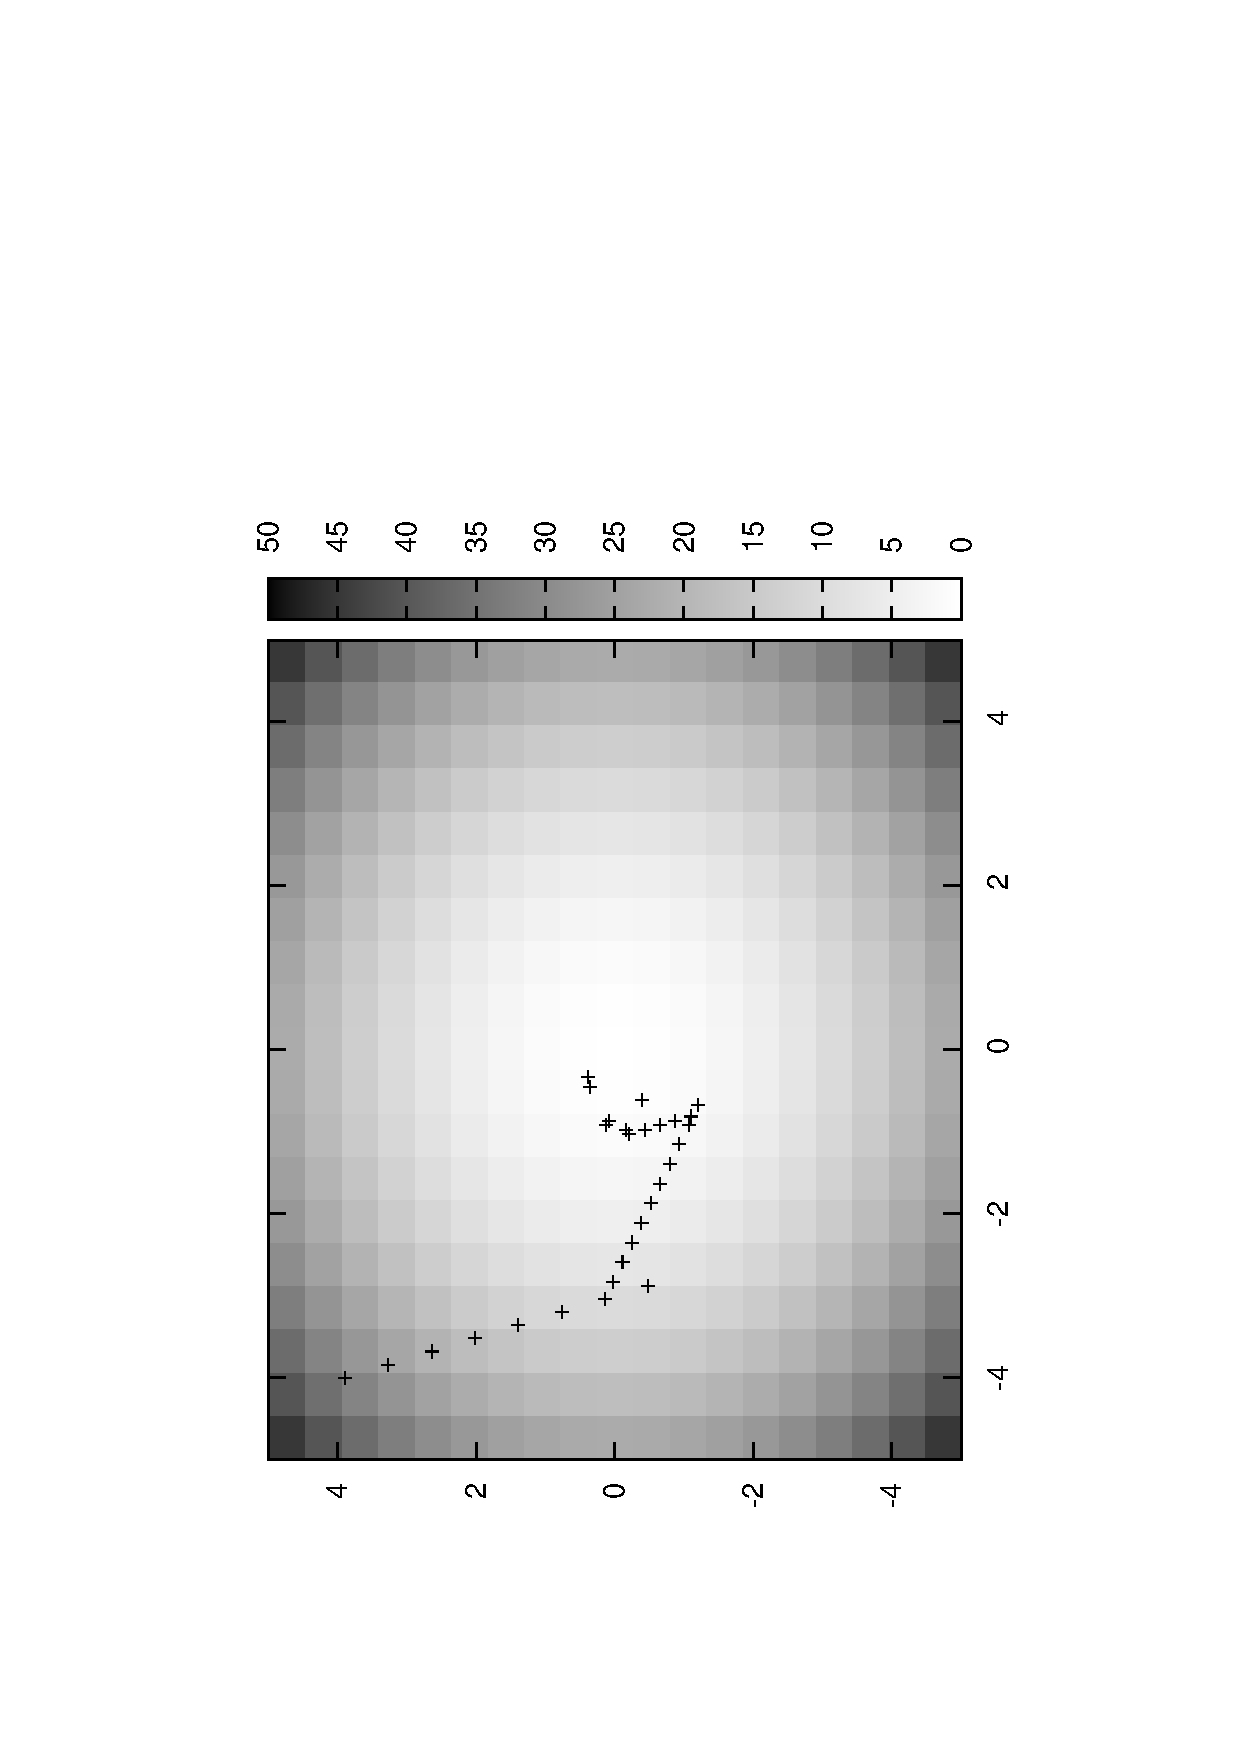
\includegraphics[trim = 2in 1.5in 2in 1.5in, clip, scale=0.5]{graphics/pso1}
\caption{Heat map plot showing selected samples in the domain.}
\label{plot:pso1}
\end{figure}

\begin{lstlisting}[caption=Gnuplot script use to create a heat map and selected samples., label=pso1]
set xrange [-5:5]
set yrange [-5:5]
set pm3d map
set palette gray negative
set samples 20
set isosamples 20
splot x*x+y*y, "pso1.txt" using 1:2:(0) with points
\end{lstlisting}

\vspace{1cm}

\begin{lstlisting}[caption=Snippet of the \texttt{pso1.txt} file., label=pso.file]
-3.9986483808224222 3.8910758979126956 31.12966051677087
-3.838580364459159 3.266132168962991 25.402318559546302
-3.678512348095896 2.6411884400132863 20.507329470753803
-3.518444331732633 2.0162447110635817 16.44469325039336
-3.35837631536937 1.391300982113877 13.214409898464986
...
\end{lstlisting}

% Traveling Salesman Problem
\subsubsection{Traveling Salesman Problem}
% general
Visualizing the results of a combinatorial optimization can provide insight into the areas of the problem that a selected technique is handling well, or  poorly.
Candidate solutions can be visualized over the course of a run to observe how the complexity of solutions found by a technique change over time. Alternatively, the best candidate solutions can be visualized at the end of a run.

Candidate solutions for the TSP are easily visualized as tours (order of city visits) in the context of the city coordinates of the problem definition.

Figure~\ref{plot:tsp3} provides a plot of an example Nearest-Neighbor solution for the Berlin52 TSP. A Nearest-Neighbor solution is constructed by randomly selecting the first city in the tour then selecting the next city in the tour with the minimum distance to the current city until a complete tour is created.

\begin{figure}[htp]
\centering
% GNUPLOT: LaTeX picture
\setlength{\unitlength}{0.240900pt}
\ifx\plotpoint\undefined\newsavebox{\plotpoint}\fi
\sbox{\plotpoint}{\rule[-0.200pt]{0.400pt}{0.400pt}}%
\begin{picture}(1500,900)(0,0)
\sbox{\plotpoint}{\rule[-0.200pt]{0.400pt}{0.400pt}}%
\put(190.0,82.0){\rule[-0.200pt]{4.818pt}{0.400pt}}
\put(170,82){\makebox(0,0)[r]{ 0}}
\put(1430.0,82.0){\rule[-0.200pt]{4.818pt}{0.400pt}}
\put(190.0,212.0){\rule[-0.200pt]{4.818pt}{0.400pt}}
\put(170,212){\makebox(0,0)[r]{ 200}}
\put(1430.0,212.0){\rule[-0.200pt]{4.818pt}{0.400pt}}
\put(190.0,341.0){\rule[-0.200pt]{4.818pt}{0.400pt}}
\put(170,341){\makebox(0,0)[r]{ 400}}
\put(1430.0,341.0){\rule[-0.200pt]{4.818pt}{0.400pt}}
\put(190.0,471.0){\rule[-0.200pt]{4.818pt}{0.400pt}}
\put(170,471){\makebox(0,0)[r]{ 600}}
\put(1430.0,471.0){\rule[-0.200pt]{4.818pt}{0.400pt}}
\put(190.0,601.0){\rule[-0.200pt]{4.818pt}{0.400pt}}
\put(170,601){\makebox(0,0)[r]{ 800}}
\put(1430.0,601.0){\rule[-0.200pt]{4.818pt}{0.400pt}}
\put(190.0,730.0){\rule[-0.200pt]{4.818pt}{0.400pt}}
\put(170,730){\makebox(0,0)[r]{ 1000}}
\put(1430.0,730.0){\rule[-0.200pt]{4.818pt}{0.400pt}}
\put(190.0,860.0){\rule[-0.200pt]{4.818pt}{0.400pt}}
\put(170,860){\makebox(0,0)[r]{ 1200}}
\put(1430.0,860.0){\rule[-0.200pt]{4.818pt}{0.400pt}}
\put(190.0,82.0){\rule[-0.200pt]{0.400pt}{4.818pt}}
\put(190,41){\makebox(0,0){ 0}}
\put(190.0,840.0){\rule[-0.200pt]{0.400pt}{4.818pt}}
\put(330.0,82.0){\rule[-0.200pt]{0.400pt}{4.818pt}}
\put(330,41){\makebox(0,0){ 200}}
\put(330.0,840.0){\rule[-0.200pt]{0.400pt}{4.818pt}}
\put(470.0,82.0){\rule[-0.200pt]{0.400pt}{4.818pt}}
\put(470,41){\makebox(0,0){ 400}}
\put(470.0,840.0){\rule[-0.200pt]{0.400pt}{4.818pt}}
\put(610.0,82.0){\rule[-0.200pt]{0.400pt}{4.818pt}}
\put(610,41){\makebox(0,0){ 600}}
\put(610.0,840.0){\rule[-0.200pt]{0.400pt}{4.818pt}}
\put(750.0,82.0){\rule[-0.200pt]{0.400pt}{4.818pt}}
\put(750,41){\makebox(0,0){ 800}}
\put(750.0,840.0){\rule[-0.200pt]{0.400pt}{4.818pt}}
\put(890.0,82.0){\rule[-0.200pt]{0.400pt}{4.818pt}}
\put(890,41){\makebox(0,0){ 1000}}
\put(890.0,840.0){\rule[-0.200pt]{0.400pt}{4.818pt}}
\put(1030.0,82.0){\rule[-0.200pt]{0.400pt}{4.818pt}}
\put(1030,41){\makebox(0,0){ 1200}}
\put(1030.0,840.0){\rule[-0.200pt]{0.400pt}{4.818pt}}
\put(1170.0,82.0){\rule[-0.200pt]{0.400pt}{4.818pt}}
\put(1170,41){\makebox(0,0){ 1400}}
\put(1170.0,840.0){\rule[-0.200pt]{0.400pt}{4.818pt}}
\put(1310.0,82.0){\rule[-0.200pt]{0.400pt}{4.818pt}}
\put(1310,41){\makebox(0,0){ 1600}}
\put(1310.0,840.0){\rule[-0.200pt]{0.400pt}{4.818pt}}
\put(1450.0,82.0){\rule[-0.200pt]{0.400pt}{4.818pt}}
\put(1450,41){\makebox(0,0){ 1800}}
\put(1450.0,840.0){\rule[-0.200pt]{0.400pt}{4.818pt}}
\put(190.0,82.0){\rule[-0.200pt]{0.400pt}{187.420pt}}
\put(190.0,82.0){\rule[-0.200pt]{303.534pt}{0.400pt}}
\put(1450.0,82.0){\rule[-0.200pt]{0.400pt}{187.420pt}}
\put(190.0,860.0){\rule[-0.200pt]{303.534pt}{0.400pt}}
\put(522,704){\usebox{\plotpoint}}
\multiput(522.00,704.58)(0.674,0.497){49}{\rule{0.638pt}{0.120pt}}
\multiput(522.00,703.17)(33.675,26.000){2}{\rule{0.319pt}{0.400pt}}
\multiput(555.92,716.14)(-0.491,-4.196){17}{\rule{0.118pt}{3.340pt}}
\multiput(556.17,723.07)(-10.000,-74.068){2}{\rule{0.400pt}{1.670pt}}
\multiput(547.58,646.50)(0.497,-0.629){59}{\rule{0.120pt}{0.603pt}}
\multiput(546.17,647.75)(31.000,-37.748){2}{\rule{0.400pt}{0.302pt}}
\multiput(578.58,598.08)(0.494,-3.545){25}{\rule{0.119pt}{2.871pt}}
\multiput(577.17,604.04)(14.000,-91.040){2}{\rule{0.400pt}{1.436pt}}
\multiput(592.58,510.53)(0.496,-0.619){39}{\rule{0.119pt}{0.595pt}}
\multiput(591.17,511.76)(21.000,-24.765){2}{\rule{0.400pt}{0.298pt}}
\multiput(611.92,484.69)(-0.497,-0.571){53}{\rule{0.120pt}{0.557pt}}
\multiput(612.17,485.84)(-28.000,-30.844){2}{\rule{0.400pt}{0.279pt}}
\multiput(576.01,455.59)(-2.751,0.482){9}{\rule{2.167pt}{0.116pt}}
\multiput(580.50,454.17)(-26.503,6.000){2}{\rule{1.083pt}{0.400pt}}
\multiput(547.47,459.92)(-1.867,-0.495){35}{\rule{1.574pt}{0.119pt}}
\multiput(550.73,460.17)(-66.734,-19.000){2}{\rule{0.787pt}{0.400pt}}
\multiput(482.94,442.00)(-0.468,7.500){5}{\rule{0.113pt}{5.300pt}}
\multiput(483.17,442.00)(-4.000,41.000){2}{\rule{0.400pt}{2.650pt}}
\multiput(478.92,494.00)(-0.498,0.756){95}{\rule{0.120pt}{0.704pt}}
\multiput(479.17,494.00)(-49.000,72.539){2}{\rule{0.400pt}{0.352pt}}
\multiput(426.36,566.92)(-1.277,-0.499){107}{\rule{1.118pt}{0.120pt}}
\multiput(428.68,567.17)(-137.679,-55.000){2}{\rule{0.559pt}{0.400pt}}
\multiput(291.58,510.60)(0.499,-0.596){215}{\rule{0.120pt}{0.577pt}}
\multiput(290.17,511.80)(109.000,-128.802){2}{\rule{0.400pt}{0.289pt}}
\multiput(400.00,381.92)(1.984,-0.497){61}{\rule{1.675pt}{0.120pt}}
\multiput(400.00,382.17)(122.523,-32.000){2}{\rule{0.838pt}{0.400pt}}
\multiput(526.00,349.92)(0.878,-0.497){61}{\rule{0.800pt}{0.120pt}}
\multiput(526.00,350.17)(54.340,-32.000){2}{\rule{0.400pt}{0.400pt}}
\multiput(582.00,317.94)(3.406,-0.468){5}{\rule{2.500pt}{0.113pt}}
\multiput(582.00,318.17)(18.811,-4.000){2}{\rule{1.250pt}{0.400pt}}
\multiput(606.00,315.59)(6.900,0.485){11}{\rule{5.300pt}{0.117pt}}
\multiput(606.00,314.17)(80.000,7.000){2}{\rule{2.650pt}{0.400pt}}
\multiput(695.92,322.00)(-0.495,2.513){31}{\rule{0.119pt}{2.076pt}}
\multiput(696.17,322.00)(-17.000,79.690){2}{\rule{0.400pt}{1.038pt}}
\multiput(677.76,458.58)(-0.547,0.491){17}{\rule{0.540pt}{0.118pt}}
\multiput(678.88,457.17)(-9.879,10.000){2}{\rule{0.270pt}{0.400pt}}
\put(680.0,406.0){\rule[-0.200pt]{0.400pt}{12.527pt}}
\multiput(669.00,477.58)(0.738,0.495){31}{\rule{0.688pt}{0.119pt}}
\multiput(669.00,476.17)(23.572,17.000){2}{\rule{0.344pt}{0.400pt}}
\multiput(694.00,494.59)(1.601,0.489){15}{\rule{1.344pt}{0.118pt}}
\multiput(694.00,493.17)(25.210,9.000){2}{\rule{0.672pt}{0.400pt}}
\multiput(722.00,501.95)(5.151,-0.447){3}{\rule{3.300pt}{0.108pt}}
\multiput(722.00,502.17)(17.151,-3.000){2}{\rule{1.650pt}{0.400pt}}
\multiput(744.92,497.34)(-0.495,-0.678){31}{\rule{0.119pt}{0.641pt}}
\multiput(745.17,498.67)(-17.000,-21.669){2}{\rule{0.400pt}{0.321pt}}
\put(669.0,468.0){\rule[-0.200pt]{0.400pt}{2.168pt}}
\multiput(771.61,477.00)(0.447,2.025){3}{\rule{0.108pt}{1.433pt}}
\multiput(770.17,477.00)(3.000,7.025){2}{\rule{0.400pt}{0.717pt}}
\multiput(774.59,487.00)(0.485,1.484){11}{\rule{0.117pt}{1.243pt}}
\multiput(773.17,487.00)(7.000,17.420){2}{\rule{0.400pt}{0.621pt}}
\put(729.0,477.0){\rule[-0.200pt]{10.118pt}{0.400pt}}
\multiput(781.00,521.92)(0.972,-0.493){23}{\rule{0.869pt}{0.119pt}}
\multiput(781.00,522.17)(23.196,-13.000){2}{\rule{0.435pt}{0.400pt}}
\multiput(806.00,510.58)(1.426,0.494){29}{\rule{1.225pt}{0.119pt}}
\multiput(806.00,509.17)(42.457,16.000){2}{\rule{0.613pt}{0.400pt}}
\multiput(851.58,520.21)(0.496,-1.637){39}{\rule{0.119pt}{1.395pt}}
\multiput(850.17,523.10)(21.000,-65.104){2}{\rule{0.400pt}{0.698pt}}
\multiput(868.88,456.92)(-0.816,-0.499){121}{\rule{0.752pt}{0.120pt}}
\multiput(870.44,457.17)(-99.440,-62.000){2}{\rule{0.376pt}{0.400pt}}
\multiput(769.92,392.84)(-0.499,-0.828){235}{\rule{0.120pt}{0.762pt}}
\multiput(770.17,394.42)(-119.000,-195.418){2}{\rule{0.400pt}{0.381pt}}
\multiput(645.13,199.58)(-1.955,0.498){87}{\rule{1.656pt}{0.120pt}}
\multiput(648.56,198.17)(-171.564,45.000){2}{\rule{0.828pt}{0.400pt}}
\multiput(424.16,244.59)(-16.816,0.485){11}{\rule{12.729pt}{0.117pt}}
\multiput(450.58,243.17)(-194.581,7.000){2}{\rule{6.364pt}{0.400pt}}
\multiput(251.52,249.92)(-1.237,-0.496){37}{\rule{1.080pt}{0.119pt}}
\multiput(253.76,250.17)(-46.758,-20.000){2}{\rule{0.540pt}{0.400pt}}
\put(781.0,507.0){\rule[-0.200pt]{0.400pt}{3.854pt}}
\multiput(207.00,202.58)(0.625,0.500){949}{\rule{0.600pt}{0.120pt}}
\multiput(207.00,201.17)(593.755,476.000){2}{\rule{0.300pt}{0.400pt}}
\multiput(799.68,678.58)(-0.573,0.499){271}{\rule{0.558pt}{0.120pt}}
\multiput(800.84,677.17)(-155.841,137.000){2}{\rule{0.279pt}{0.400pt}}
\multiput(641.78,815.58)(-0.848,0.497){55}{\rule{0.776pt}{0.120pt}}
\multiput(643.39,814.17)(-47.390,29.000){2}{\rule{0.388pt}{0.400pt}}
\multiput(596.00,842.92)(20.771,-0.491){17}{\rule{16.060pt}{0.118pt}}
\multiput(596.00,843.17)(365.667,-10.000){2}{\rule{8.030pt}{0.400pt}}
\multiput(995.58,830.06)(0.499,-1.061){263}{\rule{0.120pt}{0.948pt}}
\multiput(994.17,832.03)(133.000,-280.032){2}{\rule{0.400pt}{0.474pt}}
\multiput(1126.92,549.73)(-0.499,-0.559){165}{\rule{0.120pt}{0.548pt}}
\multiput(1127.17,550.86)(-84.000,-92.863){2}{\rule{0.400pt}{0.274pt}}
\multiput(1044.58,448.33)(0.496,-2.825){39}{\rule{0.119pt}{2.329pt}}
\multiput(1043.17,453.17)(21.000,-112.167){2}{\rule{0.400pt}{1.164pt}}
\multiput(1065.58,338.72)(0.498,-0.561){95}{\rule{0.120pt}{0.549pt}}
\multiput(1064.17,339.86)(49.000,-53.861){2}{\rule{0.400pt}{0.274pt}}
\multiput(1110.85,284.92)(-0.824,-0.498){87}{\rule{0.758pt}{0.120pt}}
\multiput(1112.43,285.17)(-72.427,-45.000){2}{\rule{0.379pt}{0.400pt}}
\multiput(1038.92,234.32)(-0.497,-1.902){59}{\rule{0.120pt}{1.610pt}}
\multiput(1039.17,237.66)(-31.000,-113.659){2}{\rule{0.400pt}{0.805pt}}
\multiput(1009.00,124.58)(1.173,0.499){173}{\rule{1.036pt}{0.120pt}}
\multiput(1009.00,123.17)(203.849,88.000){2}{\rule{0.518pt}{0.400pt}}
\multiput(1215.58,207.00)(0.498,-1.386){89}{\rule{0.120pt}{1.204pt}}
\multiput(1214.17,209.50)(46.000,-124.500){2}{\rule{0.400pt}{0.602pt}}
\multiput(1261.58,85.00)(0.499,0.530){291}{\rule{0.120pt}{0.524pt}}
\multiput(1260.17,85.00)(147.000,154.911){2}{\rule{0.400pt}{0.262pt}}
\multiput(1406.92,241.00)(-0.499,1.281){187}{\rule{0.120pt}{1.123pt}}
\multiput(1407.17,241.00)(-95.000,240.669){2}{\rule{0.400pt}{0.562pt}}
\multiput(1306.61,484.58)(-1.800,0.500){437}{\rule{1.538pt}{0.120pt}}
\multiput(1309.81,483.17)(-787.807,220.000){2}{\rule{0.769pt}{0.400pt}}
\put(522,704){\raisebox{-.8pt}{\makebox(0,0){$\Diamond$}}}
\put(557,730){\raisebox{-.8pt}{\makebox(0,0){$\Diamond$}}}
\put(547,649){\raisebox{-.8pt}{\makebox(0,0){$\Diamond$}}}
\put(578,610){\raisebox{-.8pt}{\makebox(0,0){$\Diamond$}}}
\put(592,513){\raisebox{-.8pt}{\makebox(0,0){$\Diamond$}}}
\put(613,487){\raisebox{-.8pt}{\makebox(0,0){$\Diamond$}}}
\put(585,455){\raisebox{-.8pt}{\makebox(0,0){$\Diamond$}}}
\put(554,461){\raisebox{-.8pt}{\makebox(0,0){$\Diamond$}}}
\put(484,442){\raisebox{-.8pt}{\makebox(0,0){$\Diamond$}}}
\put(480,494){\raisebox{-.8pt}{\makebox(0,0){$\Diamond$}}}
\put(431,568){\raisebox{-.8pt}{\makebox(0,0){$\Diamond$}}}
\put(291,513){\raisebox{-.8pt}{\makebox(0,0){$\Diamond$}}}
\put(400,383){\raisebox{-.8pt}{\makebox(0,0){$\Diamond$}}}
\put(526,351){\raisebox{-.8pt}{\makebox(0,0){$\Diamond$}}}
\put(582,319){\raisebox{-.8pt}{\makebox(0,0){$\Diamond$}}}
\put(606,315){\raisebox{-.8pt}{\makebox(0,0){$\Diamond$}}}
\put(697,322){\raisebox{-.8pt}{\makebox(0,0){$\Diamond$}}}
\put(680,406){\raisebox{-.8pt}{\makebox(0,0){$\Diamond$}}}
\put(680,458){\raisebox{-.8pt}{\makebox(0,0){$\Diamond$}}}
\put(669,468){\raisebox{-.8pt}{\makebox(0,0){$\Diamond$}}}
\put(669,477){\raisebox{-.8pt}{\makebox(0,0){$\Diamond$}}}
\put(694,494){\raisebox{-.8pt}{\makebox(0,0){$\Diamond$}}}
\put(722,503){\raisebox{-.8pt}{\makebox(0,0){$\Diamond$}}}
\put(746,500){\raisebox{-.8pt}{\makebox(0,0){$\Diamond$}}}
\put(729,477){\raisebox{-.8pt}{\makebox(0,0){$\Diamond$}}}
\put(771,477){\raisebox{-.8pt}{\makebox(0,0){$\Diamond$}}}
\put(774,487){\raisebox{-.8pt}{\makebox(0,0){$\Diamond$}}}
\put(781,507){\raisebox{-.8pt}{\makebox(0,0){$\Diamond$}}}
\put(781,523){\raisebox{-.8pt}{\makebox(0,0){$\Diamond$}}}
\put(806,510){\raisebox{-.8pt}{\makebox(0,0){$\Diamond$}}}
\put(851,526){\raisebox{-.8pt}{\makebox(0,0){$\Diamond$}}}
\put(872,458){\raisebox{-.8pt}{\makebox(0,0){$\Diamond$}}}
\put(771,396){\raisebox{-.8pt}{\makebox(0,0){$\Diamond$}}}
\put(652,199){\raisebox{-.8pt}{\makebox(0,0){$\Diamond$}}}
\put(477,244){\raisebox{-.8pt}{\makebox(0,0){$\Diamond$}}}
\put(256,251){\raisebox{-.8pt}{\makebox(0,0){$\Diamond$}}}
\put(207,231){\raisebox{-.8pt}{\makebox(0,0){$\Diamond$}}}
\put(207,202){\raisebox{-.8pt}{\makebox(0,0){$\Diamond$}}}
\put(802,678){\raisebox{-.8pt}{\makebox(0,0){$\Diamond$}}}
\put(645,815){\raisebox{-.8pt}{\makebox(0,0){$\Diamond$}}}
\put(596,844){\raisebox{-.8pt}{\makebox(0,0){$\Diamond$}}}
\put(995,834){\raisebox{-.8pt}{\makebox(0,0){$\Diamond$}}}
\put(1128,552){\raisebox{-.8pt}{\makebox(0,0){$\Diamond$}}}
\put(1044,458){\raisebox{-.8pt}{\makebox(0,0){$\Diamond$}}}
\put(1065,341){\raisebox{-.8pt}{\makebox(0,0){$\Diamond$}}}
\put(1114,286){\raisebox{-.8pt}{\makebox(0,0){$\Diamond$}}}
\put(1040,241){\raisebox{-.8pt}{\makebox(0,0){$\Diamond$}}}
\put(1009,124){\raisebox{-.8pt}{\makebox(0,0){$\Diamond$}}}
\put(1215,212){\raisebox{-.8pt}{\makebox(0,0){$\Diamond$}}}
\put(1261,85){\raisebox{-.8pt}{\makebox(0,0){$\Diamond$}}}
\put(1408,241){\raisebox{-.8pt}{\makebox(0,0){$\Diamond$}}}
\put(1313,484){\raisebox{-.8pt}{\makebox(0,0){$\Diamond$}}}
\put(522,704){\raisebox{-.8pt}{\makebox(0,0){$\Diamond$}}}
\put(207.0,202.0){\rule[-0.200pt]{0.400pt}{6.986pt}}
\put(190.0,82.0){\rule[-0.200pt]{0.400pt}{187.420pt}}
\put(190.0,82.0){\rule[-0.200pt]{303.534pt}{0.400pt}}
\put(1450.0,82.0){\rule[-0.200pt]{0.400pt}{187.420pt}}
\put(190.0,860.0){\rule[-0.200pt]{303.534pt}{0.400pt}}
\end{picture}

\caption{Plot of a Nearest-Neighbor tour for the Berlin52 TSP.}
\label{plot:tsp3}
\end{figure}

Listing~\ref{tsp3} provides the Gnuplot script used to prepare the plot, where \texttt{berlin52.nn.tour} is a file that contains a listing of the coordinates of all cities separated by white space in order that the cities are visited with one city per line. The first city in the tour is repeated as the last city in the tour to provide a closed polygon in the plot.
Listing~\ref{tsp3.file} provides a snippet of the first five lines of the \texttt{berlin52.nn.tour} file.

\begin{lstlisting}[caption=Gnuplot script for plotting a tour for a TSP., label=tsp3]
plot "berlin52.nn.tour" with linespoints
\end{lstlisting}

\begin{lstlisting}[caption=Snippet of the berlin52.nn.tour file., label=tsp3.file]
475 960
525 1000
510 875
555 815
575 665
...
\end{lstlisting}

Figure~\ref{plot:tsp2} provides a plot of the known optimal solution for the Berlin52 Traveling Salesman problem.

\begin{figure}[htp]
\centering
% GNUPLOT: LaTeX picture
\setlength{\unitlength}{0.240900pt}
\ifx\plotpoint\undefined\newsavebox{\plotpoint}\fi
\sbox{\plotpoint}{\rule[-0.200pt]{0.400pt}{0.400pt}}%
\begin{picture}(1200,900)(0,0)
\sbox{\plotpoint}{\rule[-0.200pt]{0.400pt}{0.400pt}}%
\put(190.0,82.0){\rule[-0.200pt]{4.818pt}{0.400pt}}
\put(170,82){\makebox(0,0)[r]{ 0}}
\put(1130.0,82.0){\rule[-0.200pt]{4.818pt}{0.400pt}}
\put(190.0,212.0){\rule[-0.200pt]{4.818pt}{0.400pt}}
\put(170,212){\makebox(0,0)[r]{ 200}}
\put(1130.0,212.0){\rule[-0.200pt]{4.818pt}{0.400pt}}
\put(190.0,341.0){\rule[-0.200pt]{4.818pt}{0.400pt}}
\put(170,341){\makebox(0,0)[r]{ 400}}
\put(1130.0,341.0){\rule[-0.200pt]{4.818pt}{0.400pt}}
\put(190.0,471.0){\rule[-0.200pt]{4.818pt}{0.400pt}}
\put(170,471){\makebox(0,0)[r]{ 600}}
\put(1130.0,471.0){\rule[-0.200pt]{4.818pt}{0.400pt}}
\put(190.0,601.0){\rule[-0.200pt]{4.818pt}{0.400pt}}
\put(170,601){\makebox(0,0)[r]{ 800}}
\put(1130.0,601.0){\rule[-0.200pt]{4.818pt}{0.400pt}}
\put(190.0,730.0){\rule[-0.200pt]{4.818pt}{0.400pt}}
\put(170,730){\makebox(0,0)[r]{ 1000}}
\put(1130.0,730.0){\rule[-0.200pt]{4.818pt}{0.400pt}}
\put(190.0,860.0){\rule[-0.200pt]{4.818pt}{0.400pt}}
\put(170,860){\makebox(0,0)[r]{ 1200}}
\put(1130.0,860.0){\rule[-0.200pt]{4.818pt}{0.400pt}}
\put(190.0,82.0){\rule[-0.200pt]{0.400pt}{4.818pt}}
\put(190,41){\makebox(0,0){ 0}}
\put(190.0,840.0){\rule[-0.200pt]{0.400pt}{4.818pt}}
\put(297.0,82.0){\rule[-0.200pt]{0.400pt}{4.818pt}}
\put(297,41){\makebox(0,0){ 200}}
\put(297.0,840.0){\rule[-0.200pt]{0.400pt}{4.818pt}}
\put(403.0,82.0){\rule[-0.200pt]{0.400pt}{4.818pt}}
\put(403,41){\makebox(0,0){ 400}}
\put(403.0,840.0){\rule[-0.200pt]{0.400pt}{4.818pt}}
\put(510.0,82.0){\rule[-0.200pt]{0.400pt}{4.818pt}}
\put(510,41){\makebox(0,0){ 600}}
\put(510.0,840.0){\rule[-0.200pt]{0.400pt}{4.818pt}}
\put(617.0,82.0){\rule[-0.200pt]{0.400pt}{4.818pt}}
\put(617,41){\makebox(0,0){ 800}}
\put(617.0,840.0){\rule[-0.200pt]{0.400pt}{4.818pt}}
\put(723.0,82.0){\rule[-0.200pt]{0.400pt}{4.818pt}}
\put(723,41){\makebox(0,0){ 1000}}
\put(723.0,840.0){\rule[-0.200pt]{0.400pt}{4.818pt}}
\put(830.0,82.0){\rule[-0.200pt]{0.400pt}{4.818pt}}
\put(830,41){\makebox(0,0){ 1200}}
\put(830.0,840.0){\rule[-0.200pt]{0.400pt}{4.818pt}}
\put(937.0,82.0){\rule[-0.200pt]{0.400pt}{4.818pt}}
\put(937,41){\makebox(0,0){ 1400}}
\put(937.0,840.0){\rule[-0.200pt]{0.400pt}{4.818pt}}
\put(1043.0,82.0){\rule[-0.200pt]{0.400pt}{4.818pt}}
\put(1043,41){\makebox(0,0){ 1600}}
\put(1043.0,840.0){\rule[-0.200pt]{0.400pt}{4.818pt}}
\put(1150.0,82.0){\rule[-0.200pt]{0.400pt}{4.818pt}}
\put(1150,41){\makebox(0,0){ 1800}}
\put(1150.0,840.0){\rule[-0.200pt]{0.400pt}{4.818pt}}
\put(190.0,82.0){\rule[-0.200pt]{0.400pt}{187.420pt}}
\put(190.0,82.0){\rule[-0.200pt]{231.264pt}{0.400pt}}
\put(1150.0,82.0){\rule[-0.200pt]{0.400pt}{187.420pt}}
\put(190.0,860.0){\rule[-0.200pt]{231.264pt}{0.400pt}}
\put(491,455){\usebox{\plotpoint}}
\multiput(491.58,455.00)(0.496,0.729){41}{\rule{0.120pt}{0.682pt}}
\multiput(490.17,455.00)(22.000,30.585){2}{\rule{0.400pt}{0.341pt}}
\multiput(511.92,487.00)(-0.494,0.817){29}{\rule{0.119pt}{0.750pt}}
\multiput(512.17,487.00)(-16.000,24.443){2}{\rule{0.400pt}{0.375pt}}
\multiput(495.92,513.00)(-0.492,4.552){19}{\rule{0.118pt}{3.627pt}}
\multiput(496.17,513.00)(-11.000,89.471){2}{\rule{0.400pt}{1.814pt}}
\multiput(484.92,610.00)(-0.496,0.816){45}{\rule{0.120pt}{0.750pt}}
\multiput(485.17,610.00)(-24.000,37.443){2}{\rule{0.400pt}{0.375pt}}
\multiput(460.92,649.00)(-0.495,1.464){35}{\rule{0.119pt}{1.258pt}}
\multiput(461.17,649.00)(-19.000,52.389){2}{\rule{0.400pt}{0.629pt}}
\multiput(443.00,704.58)(0.518,0.497){49}{\rule{0.515pt}{0.120pt}}
\multiput(443.00,703.17)(25.930,26.000){2}{\rule{0.258pt}{0.400pt}}
\multiput(470.58,730.00)(0.497,1.983){55}{\rule{0.120pt}{1.672pt}}
\multiput(469.17,730.00)(29.000,110.529){2}{\rule{0.400pt}{0.836pt}}
\multiput(499.00,842.92)(0.656,-0.497){55}{\rule{0.624pt}{0.120pt}}
\multiput(499.00,843.17)(36.705,-29.000){2}{\rule{0.312pt}{0.400pt}}
\multiput(537.58,812.69)(0.499,-0.571){237}{\rule{0.120pt}{0.557pt}}
\multiput(536.17,813.84)(120.000,-135.845){2}{\rule{0.400pt}{0.278pt}}
\multiput(657.58,678.00)(0.499,0.534){289}{\rule{0.120pt}{0.527pt}}
\multiput(656.17,678.00)(146.000,154.905){2}{\rule{0.400pt}{0.264pt}}
\multiput(803.58,828.99)(0.499,-1.385){201}{\rule{0.120pt}{1.206pt}}
\multiput(802.17,831.50)(102.000,-279.497){2}{\rule{0.400pt}{0.603pt}}
\multiput(905.00,550.92)(1.039,-0.499){133}{\rule{0.929pt}{0.120pt}}
\multiput(905.00,551.17)(139.071,-68.000){2}{\rule{0.465pt}{0.400pt}}
\multiput(1046.58,477.98)(0.499,-1.693){141}{\rule{0.120pt}{1.450pt}}
\multiput(1045.17,480.99)(72.000,-239.990){2}{\rule{0.400pt}{0.725pt}}
\multiput(1116.92,238.27)(-0.499,-0.697){221}{\rule{0.120pt}{0.657pt}}
\multiput(1117.17,239.64)(-112.000,-154.636){2}{\rule{0.400pt}{0.329pt}}
\multiput(1004.92,85.00)(-0.498,1.827){67}{\rule{0.120pt}{1.551pt}}
\multiput(1005.17,85.00)(-35.000,123.780){2}{\rule{0.400pt}{0.776pt}}
\multiput(967.62,210.92)(-0.893,-0.499){173}{\rule{0.814pt}{0.120pt}}
\multiput(969.31,211.17)(-155.311,-88.000){2}{\rule{0.407pt}{0.400pt}}
\multiput(814.58,124.00)(0.496,2.466){45}{\rule{0.120pt}{2.050pt}}
\multiput(813.17,124.00)(24.000,112.745){2}{\rule{0.400pt}{1.025pt}}
\multiput(838.00,241.58)(0.622,0.498){87}{\rule{0.598pt}{0.120pt}}
\multiput(838.00,240.17)(54.759,45.000){2}{\rule{0.299pt}{0.400pt}}
\multiput(892.92,286.00)(-0.498,0.745){71}{\rule{0.120pt}{0.695pt}}
\multiput(893.17,286.00)(-37.000,53.558){2}{\rule{0.400pt}{0.347pt}}
\multiput(855.92,341.00)(-0.494,3.730){29}{\rule{0.119pt}{3.025pt}}
\multiput(856.17,341.00)(-16.000,110.721){2}{\rule{0.400pt}{1.513pt}}
\multiput(708.92,458.00)(-0.494,2.162){29}{\rule{0.119pt}{1.800pt}}
\multiput(709.17,458.00)(-16.000,64.264){2}{\rule{0.400pt}{0.900pt}}
\multiput(689.95,524.92)(-1.105,-0.494){29}{\rule{0.975pt}{0.119pt}}
\multiput(691.98,525.17)(-32.976,-16.000){2}{\rule{0.488pt}{0.400pt}}
\multiput(656.29,510.58)(-0.695,0.493){23}{\rule{0.654pt}{0.119pt}}
\multiput(657.64,509.17)(-16.643,13.000){2}{\rule{0.327pt}{0.400pt}}
\put(710.0,458.0){\rule[-0.200pt]{31.558pt}{0.400pt}}
\multiput(639.93,501.05)(-0.482,-1.756){9}{\rule{0.116pt}{1.433pt}}
\multiput(640.17,504.03)(-6.000,-17.025){2}{\rule{0.400pt}{0.717pt}}
\put(633.17,477){\rule{0.400pt}{2.100pt}}
\multiput(634.17,482.64)(-2.000,-5.641){2}{\rule{0.400pt}{1.050pt}}
\multiput(631.92,477.00)(-0.495,0.605){35}{\rule{0.119pt}{0.584pt}}
\multiput(632.17,477.00)(-19.000,21.787){2}{\rule{0.400pt}{0.292pt}}
\multiput(612.92,496.65)(-0.493,-0.893){23}{\rule{0.119pt}{0.808pt}}
\multiput(613.17,498.32)(-13.000,-21.324){2}{\rule{0.400pt}{0.404pt}}
\multiput(599.93,477.00)(-0.482,2.299){9}{\rule{0.116pt}{1.833pt}}
\multiput(600.17,477.00)(-6.000,22.195){2}{\rule{0.400pt}{0.917pt}}
\multiput(590.71,501.93)(-1.194,-0.489){15}{\rule{1.033pt}{0.118pt}}
\multiput(592.86,502.17)(-18.855,-9.000){2}{\rule{0.517pt}{0.400pt}}
\multiput(571.73,492.92)(-0.558,-0.495){31}{\rule{0.547pt}{0.119pt}}
\multiput(572.86,493.17)(-17.865,-17.000){2}{\rule{0.274pt}{0.400pt}}
\put(641.0,507.0){\rule[-0.200pt]{0.400pt}{3.854pt}}
\multiput(555.59,465.51)(0.488,-0.626){13}{\rule{0.117pt}{0.600pt}}
\multiput(554.17,466.75)(8.000,-8.755){2}{\rule{0.400pt}{0.300pt}}
\put(555.0,468.0){\rule[-0.200pt]{0.400pt}{2.168pt}}
\multiput(563.00,404.92)(3.623,-0.491){17}{\rule{2.900pt}{0.118pt}}
\multiput(563.00,405.17)(63.981,-10.000){2}{\rule{1.450pt}{0.400pt}}
\multiput(631.92,393.39)(-0.499,-0.661){109}{\rule{0.120pt}{0.629pt}}
\multiput(632.17,394.70)(-56.000,-72.695){2}{\rule{0.400pt}{0.314pt}}
\multiput(575.92,315.75)(-0.498,-1.769){67}{\rule{0.120pt}{1.506pt}}
\multiput(576.17,318.87)(-35.000,-119.875){2}{\rule{0.400pt}{0.753pt}}
\multiput(540.92,199.00)(-0.498,1.668){67}{\rule{0.120pt}{1.426pt}}
\multiput(541.17,199.00)(-35.000,113.041){2}{\rule{0.400pt}{0.713pt}}
\multiput(499.11,315.60)(-2.528,0.468){5}{\rule{1.900pt}{0.113pt}}
\multiput(503.06,314.17)(-14.056,4.000){2}{\rule{0.950pt}{0.400pt}}
\multiput(486.35,319.58)(-0.673,0.497){61}{\rule{0.637pt}{0.120pt}}
\multiput(487.68,318.17)(-41.677,32.000){2}{\rule{0.319pt}{0.400pt}}
\multiput(444.92,345.78)(-0.498,-1.454){71}{\rule{0.120pt}{1.257pt}}
\multiput(445.17,348.39)(-37.000,-104.392){2}{\rule{0.400pt}{0.628pt}}
\multiput(400.44,242.92)(-2.468,-0.498){81}{\rule{2.062pt}{0.120pt}}
\multiput(404.72,243.17)(-201.720,-42.000){2}{\rule{1.031pt}{0.400pt}}
\put(563.0,406.0){\rule[-0.200pt]{0.400pt}{12.527pt}}
\multiput(203.00,231.58)(0.956,0.496){37}{\rule{0.860pt}{0.119pt}}
\multiput(203.00,230.17)(36.215,20.000){2}{\rule{0.430pt}{0.400pt}}
\multiput(241.58,251.00)(0.499,0.605){215}{\rule{0.120pt}{0.584pt}}
\multiput(240.17,251.00)(109.000,130.787){2}{\rule{0.400pt}{0.292pt}}
\multiput(348.92,383.00)(-0.499,0.784){163}{\rule{0.120pt}{0.727pt}}
\multiput(349.17,383.00)(-83.000,128.492){2}{\rule{0.400pt}{0.363pt}}
\multiput(267.00,513.58)(0.975,0.499){107}{\rule{0.878pt}{0.120pt}}
\multiput(267.00,512.17)(105.177,55.000){2}{\rule{0.439pt}{0.400pt}}
\multiput(374.58,564.26)(0.498,-1.004){71}{\rule{0.120pt}{0.900pt}}
\multiput(373.17,566.13)(37.000,-72.132){2}{\rule{0.400pt}{0.450pt}}
\multiput(411.61,464.80)(0.447,-11.402){3}{\rule{0.108pt}{7.033pt}}
\multiput(410.17,479.40)(3.000,-37.402){2}{\rule{0.400pt}{3.517pt}}
\multiput(414.00,442.58)(1.410,0.495){35}{\rule{1.216pt}{0.119pt}}
\multiput(414.00,441.17)(50.477,19.000){2}{\rule{0.608pt}{0.400pt}}
\multiput(467.00,459.93)(2.118,-0.482){9}{\rule{1.700pt}{0.116pt}}
\multiput(467.00,460.17)(20.472,-6.000){2}{\rule{0.850pt}{0.400pt}}
\put(491,455){\raisebox{-.8pt}{\makebox(0,0){$\Diamond$}}}
\put(513,487){\raisebox{-.8pt}{\makebox(0,0){$\Diamond$}}}
\put(497,513){\raisebox{-.8pt}{\makebox(0,0){$\Diamond$}}}
\put(486,610){\raisebox{-.8pt}{\makebox(0,0){$\Diamond$}}}
\put(462,649){\raisebox{-.8pt}{\makebox(0,0){$\Diamond$}}}
\put(443,704){\raisebox{-.8pt}{\makebox(0,0){$\Diamond$}}}
\put(470,730){\raisebox{-.8pt}{\makebox(0,0){$\Diamond$}}}
\put(499,844){\raisebox{-.8pt}{\makebox(0,0){$\Diamond$}}}
\put(537,815){\raisebox{-.8pt}{\makebox(0,0){$\Diamond$}}}
\put(657,678){\raisebox{-.8pt}{\makebox(0,0){$\Diamond$}}}
\put(803,834){\raisebox{-.8pt}{\makebox(0,0){$\Diamond$}}}
\put(905,552){\raisebox{-.8pt}{\makebox(0,0){$\Diamond$}}}
\put(1046,484){\raisebox{-.8pt}{\makebox(0,0){$\Diamond$}}}
\put(1118,241){\raisebox{-.8pt}{\makebox(0,0){$\Diamond$}}}
\put(1006,85){\raisebox{-.8pt}{\makebox(0,0){$\Diamond$}}}
\put(971,212){\raisebox{-.8pt}{\makebox(0,0){$\Diamond$}}}
\put(814,124){\raisebox{-.8pt}{\makebox(0,0){$\Diamond$}}}
\put(838,241){\raisebox{-.8pt}{\makebox(0,0){$\Diamond$}}}
\put(894,286){\raisebox{-.8pt}{\makebox(0,0){$\Diamond$}}}
\put(857,341){\raisebox{-.8pt}{\makebox(0,0){$\Diamond$}}}
\put(841,458){\raisebox{-.8pt}{\makebox(0,0){$\Diamond$}}}
\put(710,458){\raisebox{-.8pt}{\makebox(0,0){$\Diamond$}}}
\put(694,526){\raisebox{-.8pt}{\makebox(0,0){$\Diamond$}}}
\put(659,510){\raisebox{-.8pt}{\makebox(0,0){$\Diamond$}}}
\put(641,523){\raisebox{-.8pt}{\makebox(0,0){$\Diamond$}}}
\put(641,507){\raisebox{-.8pt}{\makebox(0,0){$\Diamond$}}}
\put(635,487){\raisebox{-.8pt}{\makebox(0,0){$\Diamond$}}}
\put(633,477){\raisebox{-.8pt}{\makebox(0,0){$\Diamond$}}}
\put(614,500){\raisebox{-.8pt}{\makebox(0,0){$\Diamond$}}}
\put(601,477){\raisebox{-.8pt}{\makebox(0,0){$\Diamond$}}}
\put(595,503){\raisebox{-.8pt}{\makebox(0,0){$\Diamond$}}}
\put(574,494){\raisebox{-.8pt}{\makebox(0,0){$\Diamond$}}}
\put(555,477){\raisebox{-.8pt}{\makebox(0,0){$\Diamond$}}}
\put(555,468){\raisebox{-.8pt}{\makebox(0,0){$\Diamond$}}}
\put(563,458){\raisebox{-.8pt}{\makebox(0,0){$\Diamond$}}}
\put(563,406){\raisebox{-.8pt}{\makebox(0,0){$\Diamond$}}}
\put(633,396){\raisebox{-.8pt}{\makebox(0,0){$\Diamond$}}}
\put(577,322){\raisebox{-.8pt}{\makebox(0,0){$\Diamond$}}}
\put(542,199){\raisebox{-.8pt}{\makebox(0,0){$\Diamond$}}}
\put(507,315){\raisebox{-.8pt}{\makebox(0,0){$\Diamond$}}}
\put(489,319){\raisebox{-.8pt}{\makebox(0,0){$\Diamond$}}}
\put(446,351){\raisebox{-.8pt}{\makebox(0,0){$\Diamond$}}}
\put(409,244){\raisebox{-.8pt}{\makebox(0,0){$\Diamond$}}}
\put(203,202){\raisebox{-.8pt}{\makebox(0,0){$\Diamond$}}}
\put(203,231){\raisebox{-.8pt}{\makebox(0,0){$\Diamond$}}}
\put(241,251){\raisebox{-.8pt}{\makebox(0,0){$\Diamond$}}}
\put(350,383){\raisebox{-.8pt}{\makebox(0,0){$\Diamond$}}}
\put(267,513){\raisebox{-.8pt}{\makebox(0,0){$\Diamond$}}}
\put(374,568){\raisebox{-.8pt}{\makebox(0,0){$\Diamond$}}}
\put(411,494){\raisebox{-.8pt}{\makebox(0,0){$\Diamond$}}}
\put(414,442){\raisebox{-.8pt}{\makebox(0,0){$\Diamond$}}}
\put(467,461){\raisebox{-.8pt}{\makebox(0,0){$\Diamond$}}}
\put(491,455){\raisebox{-.8pt}{\makebox(0,0){$\Diamond$}}}
\put(203.0,202.0){\rule[-0.200pt]{0.400pt}{6.986pt}}
\put(190.0,82.0){\rule[-0.200pt]{0.400pt}{187.420pt}}
\put(190.0,82.0){\rule[-0.200pt]{231.264pt}{0.400pt}}
\put(1150.0,82.0){\rule[-0.200pt]{0.400pt}{187.420pt}}
\put(190.0,860.0){\rule[-0.200pt]{231.264pt}{0.400pt}}
\end{picture}

\caption{Plot of the optimal tour for the Berlin52 TSP.}
\label{plot:tsp2}
\end{figure}

Listing~\ref{tsp2} provides the Gnuplot script used to prepare the plot, where \texttt{berlin52.optimal} is a file that contains a listing of the coordinates of all cities in order that the cities are visited with one city per line separated by white space. The first city in the tour is repeated as the last city in the tour to provide a closed polygon in the plot.

\begin{lstlisting}[caption=Gnuplot script for plotting a tour for a TSP., label=tsp2]
plot "berlin52.optimal" with linespoints
\end{lstlisting}

Listing~\ref{tsp2.file} provides a snippet of the first five lines of the \texttt{berlin52.optimal} file.

\begin{lstlisting}[caption=Snippet of the \texttt{berlin52.optimal} file., label=tsp2.file]
565.0 575.0
605.0 625.0
575.0 665.0
555.0 815.0
510.0 875.0
...
\end{lstlisting}
\putbib\end{bibunit}
\newpage\begin{bibunit}% The Clever Algorithms Project: http://www.CleverAlgorithms.com
% (c) Copyright 2010 Jason Brownlee. Some Rights Reserved. 
% This work is licensed under a Creative Commons Attribution-Noncommercial-Share Alike 2.5 Australia License.

% Problem Solving Method
\section{Problem Solving Strategies} 
\label{advanced:sec:problem_solving}
\index{Problem Solving Strategies}

% this section
The field of Data Mining has clear methodologies that guide a practitioner to solve problems, such as Knowledge Discovery in Databases (KDD) \cite{Fayyad1996}. Metaheuristics and Computational Intelligence algorithms have no such methodology.\footnote{Some methods can be used for classification and regression and as such may fit into methodologies such as KDD.}

This section describes some of the considerations when applying algorithms from the fields of Metaheuristics, Computational Intelligence, and Biologically Inspired Computation to practical problem domains. This discussion includes:

\begin{itemize} 
  \item The suitability of application of a given technique to a given problem and the transferability of algorithm and problem features (Section~\ref{sec:suitability})
  \item The distinction between strong and weak methods which use more or less problem specific information respectively, and the continuum between these extremes (Section~\ref{sec:strong_methods}).
	\item A summary of problem solving strategies that suggest different ways of applying a given technique to the function optimization and approximation fields (Section~\ref{sec:strategies}).
\end{itemize}

%
% Suitability of Application
%
\subsection{Suitability of Application}
\label{sec:suitability}
\index{Suitability of Application}
% utility as problems solvers
From a problem-solving perspective, the tools that emerge from the field of Computational Intelligence are generally assessed with regard to their utility as \emph{efficiently} or \emph{effectively} solving problems.
% nfl
An important lesson from the No-Free-Lunch Theorem was to \emph{bound claims of applicability} (see Section~{subsec:nfl}), that is to consider the suitability of a given strategy with regard to the feature overlap with the attributes of a given problem domain. From a Computational Intelligence perspective, one may consider the architecture, processes, and constraints of a given strategy as the features of an approach. 

The suitability of the application of a particular approach to a problem takes into considerations concerns such as the \emph{appropriateness} (can the approach address the problem), the \emph{feasibility} (available resources and related efficiency concerns), and the \emph{flexibility} (ability to address unexpected or unintended effects).
% my approach
This section summarizes a general methodology toward addressing the problem of suitability in the context of Computational Intelligence tools. This methodology involves 1) the systematic elicitation of system and problem features, and 2) the consideration of the overlap of problem-problem, algorithm-algorithm, and problem-algorithm overlap of feature sets. 

% Systematic Feature Elicitation
\subsubsection{Systematic Feature Elicitation}
A \emph{feature} of a system (tool, strategy, model) or a problem is a distinctive element or property that may be used to differentiate it from similar and/or related cases. Examples may include functional concerns such as: processes, data structures, architectures, and constraints, as well as emergent concerns that may have a more subjective quality such as general behaviors, organizations, and higher-order structures. The process of the elicitation of features may be taken from a system or problem perspective:

\begin{itemize}
	\item \emph{System Perspective}: This requires a strong focus on the lower level functional elements and investigations that work toward correlating specific controlled procedures towards predictable emergent behaviors. 
	\item \emph{Problem Perspective}: May require both a generalization of the specific case to the general problem case, as well as a functional or logical decomposition into constituent parts.
\end{itemize}

Problem \emph{generalization} and \emph{functional decomposition} are important and commonly used patterns for problem solving in the broader fields of Artificial Intelligence and Machine Learning. The promotion of simplification and modularity can reduce the cost and complexity of achieving solutions \cite{Russell2009, Brooks1986}.

%
% Feature Overlap
%
\subsubsection{Feature Overlap}
% general overlap
Overlap in elicited features may be considered from three important perspectives: \emph{between systems}, \emph{between problems}, and \emph{between a system and a problem}. Further, such overlap may be considered at different levels of detail with regard to generalized problem solving strategies and problem definitions.
% cases
These overlap cases are considered as follows:

\begin{itemize}
	\item \emph{System Overlap} defines the suitability of comparing one system to another, referred to as \emph{comparability}. For example, systems may be considered for the same general problems and compared in terms of theoretical or empirical capability, the results of which may only be meaningful if the systems are significantly similar to each other as assessed in terms of feature overlap. 
	\item \emph{Problem Overlap} defines the suitability of comparing one problem to another, referred to as \emph{transferability}. From a systems focus, transferability refers to the capability of a technique on a given problem to be successfully applied to another problem, the result of which is only meaningful if there is a strong overlap between the problems under consideration.
	\item \emph{System-Problem Overlap} defines the suitability of a system on a given problem, referred to as \emph{applicability}. For example, a system is considered suitable for a given problem if it has a significant overlap in capabilities with the requirements of the problem definition.
\end{itemize}

% noise
Such mappings are imprecise given the subjective assessment and complexity required in both the elicitation and consideration overlap of the of features, the hardest of which is expected to be the mapping between systems and problems. 
% nfl
The mapping of salient features of algorithms and problems was proposed as an important reconciliation of the No-Free-Lunch Theorem by Wolpert and Macready \cite{Wolpert1997}, although the important difference of this approach is that the system and algorithm are given prior to the assessment. In their first work on the theorem, Wolpert and Macready specifically propose the elicitation of the features from a problem-first perspective, for which specialized algorithms can be defined \cite{Wolpert1995}. Therefore, this methodology of suitability may be considered a generalization of this reconciliation suitable for the altered Computational Intelligence (strategy first) perspective on Artificial Intelligence.
% this argument also supports outlining capability by analogy

%
% Strong and Weak Methods
%
\subsection{Strong and Weak Methods}
\label{sec:strong_methods}
\index{Strong and Weak Methods}
% weak
Generally, the methods from the fields of Metaheuristics, Computational Intelligence, and Biologically Inspired Computation may be considered weak methods. They are general purpose and are typically considered black-box solvers for a range of problem domains. The stronger the method, the more that must be known about the problem domain.
% weak and strong
Rather than discriminating techniques into weak and strong it is more useful to consider a continuum of methods from pure block box techniques that have few assumptions about the problem domain, to strong methods that exploit most or all of the problem specific information available.

For example, the Traveling Salesman Problem is an example of a combinatorial optimization problem. A na\"ive (such a Random Search) black box method may simply explore permutations of the cities. Slightly stronger methods may initialize the search with a heuristic-generated technique (such as nearest neighbor) and explore the search space using a variation method that also exploits heuristic information about the domain (such as a 2-opt variation). Continuing along this theme, a stochastic method may explore the search space using a combination of probabilistic and heuristic information (such as Ant Colony Optimization algorithms). At the other end of the scale the stochastic elements are decreased or removed until one is left with pure heuristic methods such as  the Lin-Kernighan heuristic \cite{Lin1973} and exact algorithms from linear and dynamic programming that focus on the structure and nature of the problem \cite{Woeginger2003}.

% strategy
Approaching a problem is not as simple as selecting the strongest method available and solving it. The following describes two potential strategies:

\begin{itemize}
  \item \emph{Start Strong}: Select the strongest technique available and apply it to the problem. Difficult problems can be resistant to traditional methods for many intrinsic and extrinsic reasons. Use products from a strong technique (best solution found, heuristics) to seed the next weaker method in line. 
  \item \emph{Start Weak}: Strong methods do not exist for all problems, and if they do exist, the computation, skill, and/or time resources may not be available to exploit them. Start with a weak technique and use it to learn about the problem domain. Use this information to make better decisions about subsequent techniques to try that can exploit what has been learned.
\end{itemize}

In a real-world engineering or business scenario, the objective is to solve a problem or achieve the best possible solution to the problem within the operating constraints.
Concerns of algorithm and technique purity become less important than they may be in their respective fields of research.
Both of the above strategies suggest an iterative methodology, where the product or knowledge gained from one technique may be used to prime a subsequent stronger or weaker technique. 

%
% Domain-Specific Strategies
%
\subsection{Domain-Specific Strategies}
\label{sec:strategies}
\index{Domain-Specific Strategies}
An algorithm may be considered a strategy for problem solving. There are a wide range of ways in which a given algorithm can be used to solve a problem. 
Function Optimization and Function Approximation were presented as two general classes of problems to which the algorithms from the fields of Metaheuristics, Computational Intelligence, and Biologically Inspired Computation are applied. 
This section reviews general problem problem solving strategies that may be adopted for a given technique in each of these general problem domains.

%
% Function Optimization
%
\subsubsection{Function Optimization}
\index{Function Optimization}
This section reviews a select set of strategies for addressing optimization problems from the field of Metaheuristics and Computational Intelligence to provide general insight into the state of the interaction between stochastic algorithms and the field of optimization. This section draws heavily from the field of Evolutionary Computation, Swarm Intelligence, and related Computational Intelligence sub-fields.
	
\paragraph{Global and Local Optimization}
\index{Global and Local Optimization}
\index{Function Optimization!Global and Local}
Global Optimization refers to seeking a globally optimal structure or approximation thereof in a given problem domain. Global is differentiated from Local Optimization in that the latter focuses on locating an optimal structure within a constrained region of the decision variable search space, such as a single peak or valley (basin of attraction). In the literature, global optimization problems refers to the class of optimization problems that generally cannot be addressed through more conventional approaches such as gradient descent methods (that require mathematical derivatives) and pattern search (that can get `stuck' in local optima and never converge) \cite{Price1977, Toern1999}. 

A global search strategy provides the benefit of making few if any assumptions about where promising areas of the search space may be, potentially highlighting unintuitive combinations of parameters. A local search strategy provides the benefit of focus and refinement of an existing candidate solution. It is common to apply a local search method to the solutions located by a global search procedure as a refinement strategy (such as using a Hill Climber (Section~\ref{sec:stochastic_hill_climbing}) after a Genetic Algorithm (Section~\ref{sec:genetic_algorithm})), and some methods have both techniques built in (such as GRASP in Section~\ref{sec:grasp}).
	
\paragraph{Parallel Optimization}
\index{Parallel Optimization}
\index{Function Optimization!Parallel}
A natural step toward addressing difficult (large and rugged cost landscapes) is to exploit parallel and distributed hardware, to get an improved result in the same amount of time, the same result in less time, or both \cite{Crainic2005}. Towards unifying the myriad of approaches and hardware configurations, a general consensus and taxonomy has been defined by the Parallel Evolutionary Algorithms (PEA) and Parallel Metaheuristics fields that considers the ratio of \emph{communication} to \emph{computation} called \emph{granularity} \cite{Cantu-Paz2000, Alba2005a}. 

This taxonomy is presented concisely by Alba and Tomassini as a plot or trade-off of three concerns: 1) the number of sub-populations (models or parallel strategies working on the problem), 2) the coupling between the sub-populations (frequency and amplitude of communication), and 3) the size of the sub-populations (size or extent of the sub-models) \cite{Alba2002}. 

Two important and relevant findings from the narrower field of Parallel Evolutionary Algorithms include 1) that tight coupling (frequent inter-system migration of candidate solutions) between coarse-grained models typically results in worse performance than a non-distributed approach \cite{Alba2000}, and 2) that loose coupling (infrequent migration) between coarse-grained models has been consistently shown to provide a super-linear increase in performance \cite{Alba2002a, Belding1995, Cantu-Paz2000}.
	
\paragraph{Cooperative Search}
\index{Cooperative Search}
\index{Function Optimization!Cooperative}
This is a more general approach that considers the use of multiple models that work together to address a difficult optimization problems. Durfee et~al.\ consider so-called Cooperative Distributed Problem Solving (CDPS) in which a network of loosely coupled solvers are employed to address complex distributed problems. In such systems, it is desirable to match the processing capabilities of the solver to the attributes of the problem. For example, a given problem may have spatially distributed, functionally distributed, or temporally distributed sub-problems to which a centralized and monolithic system may not be suitable. 

Lesser \cite{Lesser1990} considers CDPS and proposes such models perform \emph{distributed search} on dependent or independent and potentially overlapping sub-problems as a motivating perspective for conducting research into Distributed Artificial Intelligence (DAI)\footnote{This perspective provided the basis for what became the field of Multi-Agent Systems (MAS).}. Lesser points out that in real world applications, it is hard to get a optimal mapping between the allocated resources and the needs or availability of information for a given problem, suggesting that such problems may be caused by a mismatch in processing times and/or number of sub-problems, interdependencies between sub-problems, and local experts whose expertise cannot be effectively communicated. For a more detail on the relationships between parallel and cooperative search, El-Abd and Kamel provide a rigorous taxonomy \cite{El-Abd2005}.
	
\paragraph{Hybrid Search}
\index{Function Optimization!Hybrid}
Hybrid Search is a perspective on optimization that focuses on the use of multiple and likely different approaches either sequentially (as in the canonical global and local search case), or in parallel (such as in Cooperative Search). For example in this latter case, it is common in the field of PEA to encourage different levels of exploration and exploitation across island populations by varying the operators or operator configurations used \cite{Tanese1989, Adamidis1996}. 

Talbi proposed a detailed 4-level taxonomy of Hybrid Metaheuristics that concerns parallel and cooperating approaches \cite{Talbi2001}. The taxonomy encompasses parallel and cooperative considerations for optimization and focuses on the discriminating features in the lowest level such as heterogeneity, and specialization of approaches.
	
\paragraph{Functional Decomposition}
\index{Function Optimization!Decomposition}
Three examples of a functional decomposition of optimization include 1) multiple objectives, 2) multiple constraints, and 3) partitions of the decision variable search space. 

\index{Multi-Objective Optimization}
\index{Pareto Optimal}
\index{Pareto Front}
Multi-Objective Optimization (MOO) is a sub-field that is concerned with the optimization of two or more objective functions. A solution to a MOO conventionally involves locating and returning a set of candidate solutions called the non-dominated set \cite{Deb2001}. The Pareto optimal set, is the set of optimal non-dominated solutions. For a given problem no feasible solution exists that dominates a Pareto optimal solution. All solutions that are Pareto optimal belong to the Pareto set, and the points that these solutions map to in the objective space is called the Pareto front. The complexity with MOO problems is in the typically unknown dependencies between decision variables across objectives, that in the case of conflicts, must be traded off (Purshouse and Fleming provide a taxonomy of such complexity \cite{Purshouse2003}). 

\index{Constraint Satisfaction}
Constraint Satisfaction Problem's (CSP) involve the optimization of decision variables under a set of constraints. The principle complexity in such problems is in locating structures that are feasible or violate the least number of constraints, optimizing such feasibility \cite{Tsang1993, Kumar1992}. 

\index{Search Space Partitioning}
Search Space Partitioning involves partitioning of the decision variable search space (for example see Multispace Search by Gu et~al.\ \cite{Du1997, Gu1997, Gu1994}). This is a critical consideration given that for equal-sized dimensional bounds on parameters, an increase in decision variables results in an exponential increase in the volume of the space to search.
			
\paragraph{Availability Decomposition}
Optimization problems may be partitioned by the concerns of temporal and spatial distribution of 1) information availability, and 2) computation availability. An interesting area of research regarding variable information availability for optimization problems is called Interactive Evolutionary Computation, in which one or a collection of human operators dynamically interact with an optimization process \cite{Takagi2001}. Example problem domains include but are not limited to computer graphics, industrial design, image processing, and drug design. 

There is an increasing demand to exploit clusters of heterogeneous workstations to complete large-scale distributed computation tasks like optimization, typically in an opportunistic manner such as when individual machines are underutilized. The effect is that optimization strategies such as random partitioning of the search space (independent non-interacting processing) are required to take advantage of such environments for optimization problems \cite{Schnekenburger1993, Liu2000}.
	
\paragraph{Meta Optimization}
\index{Function Optimization!Meta}
One may optimize at a level above that considered in previous sections. Specifically, 1) the iterative generation of an inductive model called multiple restart optimization, and 2) the optimization of the parameters of the process that generates an inductive model of an optimization problem. Multiple or iterative restarts involves multiple independent algorithm executions from different (random) starting conditions. It is generally considered as a method for achieving an improved result in difficult optimization problems where a given strategy is deceived by local or false optima \cite{Muselli1997, Hu1994}, typically requiring a restart schedule \cite{Fukunaga1998}. 

A second and well studied form of meta optimization involves the optimization of the search process itself. Classical examples include the self-adaptation of mutation parameters (step sizes) in the Evolutionary Strategies (ES) and Evolutionary Programming (EP) approaches. Smith and Fogarty provided a review of genetic algorithms with adaptive strategies including a taxonomy in which the meta-adaptations are applied at one of three levels: 1) the population (adapting the overall sampling strategy), 2) the individual (adapting the creation of new samples in the decision variable space), and 3) components (modifying component contributions and/or individual step sizes as in ES and EP) \cite{Smith1997b}.



%
% Function Approximation
%
\subsubsection{Function Approximation}
\index{Function Approximation}
This section reviews a select set of strategies for addressing Function Approximation problems from the fields of Artificial Intelligence and Computational Intelligence to provide general insight into the state of the interaction between stochastic algorithms and the field. The review draws heavily from the fields of Artificial Neural Networks, specifically Competitive Learning, as well as related inductive Machine Learning fields such as Instance Based Learning.

\paragraph{Vector Quantization}
\index{Vector Quantization}
\index{Function Approximation!Vector Quantization}
Vector Quantization (VQ) refers to a method of approximating a target function using a set of exemplar (prototype or codebook) vectors. The exemplars represent a discrete subset of the problem, generally restricted to the features of interest using the natural representation of the observations in the problem space, typically an an unconstrained $n$-dimensional real valued space. The VQ method provides the advantage of a non-parametric model of a target function (like instance-based and lazy learning such as the $k$-Nearest-Neighbor method (\emph{k}NN)) using a symbolic representation that is meaningful in the domain (like tree-based approaches). 

The promotion of compression addresses the storage and retrieval concerns of \emph{k}NN, although the selection of codebook vectors (the so-called quantization problem) is a hard problem that is known to be NP-complete \cite{Garey1982}. More recently Kuncheva and Bezdek have worked towards unifying quantization methods in the application to classification problems, referring to the approaches as Nearest Prototype Classifiers (NPC) and proposing a generalized nearest prototype classifier \cite{Kuncheva1998, Kuncheva1998a}.
	
\paragraph{Parallelization} 
\index{Function Approximation!Parallelization}
Instance-based approaches are inherently parallel given the generally discrete independent nature in which they are used, specifically in a case or per-query manner. As such, parallel hardware can be exploited in the preparation of the corpus of prototypes (parallel preparation), and more so in the application of the corpus given its read-only usage \cite{Aamodt1994, Nagendra1996, Plaza1997}. With regard to vector quantization specifically, there is an industry centered around the design and development of VQ and WTA algorithms and circuits given their usage to compress digital audio and video data \cite{Nakada1999, Parhi1994}.
	
\paragraph{Cooperative Methods}
\index{Function Approximation!Cooperative}
Classical cooperative methods in the broader field of statistical machine learning are referred to as \emph{Ensemble Methods} \cite{Opitz1999, Polikar2006} or more recently \emph{Multiclassifier Systems} \cite{Ghosh2002}. 

\index{Boosting}
\emph{Boosting} is based on the principle of combining a set of quasi-independent weak learners that collectively are as effective as a single strong learner \cite{Kearns1988, Schapire1992}. The seminal approach is called Adaptive Boosting (AdaBoost) that involves the preparation of a series of classifiers, where subsequent classifiers are prepared for the observations that are misclassified by the proceeding classifier models (creation of specialists) \cite{Schapire2003}. 

\index{Bootstrap Aggregation}
\emph{Bootstrap Aggregation} (bagging) involves partitioning the observations into $N$ randomly chosen subsets (with re-selection), and training a different model on each \cite{Breiman1996}. Although robust to noisy datasets, the approach requires careful consideration as to the consensus mechanism between the independent models for decision making. 

\index{Stacked Generalization}
\emph{Stacked Generalization} (stacking) involves creating a sequence of models of generally different types arranged into a stack, where subsequently added models generalize the behavior (success or failure) of the model before it with the intent of correcting erroneous decision making \cite{Wolpert1992, Ting1999}. 
	
\paragraph{Functional Decomposition}
\index{Function Approximation!Decomposition}
As demonstrated, it is common in ensemble methods to partition the dataset either explicitly or implicitly to improve the approximation of the underlying target function. A first important decomposition involves partitioning the problem space into sub-spaces based on the attributes, regular groups of attributes called features, and decision attributes such as class labels. A popular method for attribute-based partitioning is called the Random Subspace Method, involving the random partitioning of attributes to which specialized model is prepared for each (commonly used on tree-based approaches) \cite{Ho1998}. 

A related approach involves a hierarchical partitioning of attributes space into sub-vectors (sub-spaces) used to improve VQ-based compression \cite{Gersho1984}. Another important functional decomposition methods involve the partitioning of the set of observations. The are many ways in which observations may be divided, although common approaches include pre-processing using clustering techniques to divide the set into natural groups, additional statistical approaches that partition based on central tendency and outliers, and re-sampling methods that are required to reduce the volume of observations.
	
\paragraph{Availability Decomposition}
The availability observations required to address function approximation in real-world problem domains motivate the current state of the art in Distributed Data Mining (DDM, or sometimes Collective Data Mining), Parallel Data Mining (PDM), and Distributed Knowledge Discovery in Database (DKDD) \cite{Kargupta2000}. The general information availability concerns include 1) the \emph{intractable volume of observations}, and 2) the \emph{spatial (geographical) and temporal distribution of information} \cite{Zaki1999}. In many real-world problems it is infeasible to centralize relevant observations for modeling, requiring scalable, load balancing, and incremental acquisition of information \cite{Skillicorn1999}. 
	
\paragraph{Meta-Approximation}
\index{Function Approximation!Meta}
The so-called ensemble or multiple-classifier methods may be considered meta approximation approaches as they are not specific to a given modeling technique. As with function optimization, meta-approaches may be divided into restart methods and meta-learning algorithms. The use of restart methods is a standard practice for connectionist approaches, and more generally in approaches that use random starting conditions and a gradient or local search method of refinement. 

The method provides an opportunity for over-coming local optima in the error-response surface, when there is an unknown time remaining until convergence \cite{Magdon-ismail2000}, and can exploit parallel hardware to provide a speed advantage \cite{Blas2005}. Ensemble methods and variants are examples of meta approximation approaches, as well as the use of consensus classifiers (gate networks in mixtures of experts) to integrate and weight the decision making properties from ensembles. 

\putbib\end{bibunit}
\newpage\begin{bibunit}% The Clever Algorithms Project: http://www.CleverAlgorithms.com
% (c) Copyright 2010 Jason Brownlee. Some Rights Reserved. 
% This work is licensed under a Creative Commons Attribution-Noncommercial-Share Alike 2.5 Australia License.

% Racing Algorithms
\section{Benchmarking Algorithms} 
\label{advanced:sec:racing_algorithms}
\index{Racing Algorithms}
\index{Benchmarking}

% this report
When it comes to evaluating an optimization algorithm, every researcher has their own thoughts on the way it should be done. Unfortunately, many empirical evaluations of optimization algorithms are performed and reported without addressing basic experimental design considerations. This section provides a summary of the literature on experimental design and empirical algorithm comparison methodology. This summary contains rules of thumb and the seeds of best practice when attempting to configure and compare optimization algorithms, specifically in the face of the no-free-lunch theorem.

% 
% Issues of Benchmarking Methodology
% 
\subsection{Issues of Benchmarking Methodology}
\index{Benchmarking!Issues}
Empirically	comparing	the	performance	of algorithms on optimization problem instances is a staple for the fields of Heuristics and Biologically Inspired Computation, and the problems of effective comparison methodology have been discussed since the inception of these fields. Johnson suggests that the coding of an algorithm is the easy part of the process; the difficult work is getting meaningful and publishable results \cite{Johnson2002a}. He goes on to provide a very through list of questions to consider before racing algorithms, as well as what he describes as his ``pet peeves'' within the field of empirical algorithm research.

Hooker \cite{Hooker1995} (among others) practically condemns what he refers to as competitive testing of heuristic algorithms, calling it ``\emph{fundamentally anti-intellectual}''. He goes on to strongly encourage a rigorous methodology of what he refers to as scientific testing where the aim is to investigate algorithmic behaviors. 

Barr, Golden et~al.\ \cite{Barr1995} list a number of properties worthy of a heuristic method making a contribution, which can be paraphrased as; efficiency, efficacy, robustness, complexity, impact, generalizability, and innovation. This is interesting given that many (perhaps a majority) of conference papers focus on solution quality alone (one aspect of efficacy).
In their classical work on reporting empirical results of heuristics Barr, Golden et~al.\ specify a loose experimental setup methodology with the following steps:

\begin{enumerate}
	\item Define the goals of the experiment.
	\item Select measure of performance and factors to explore.
	\item Design and execute the experiment.
	\item Analyze the data and draw conclusions.
	\item Report the experimental results.
\end{enumerate}

They then suggest eight guidelines for reporting results, in summary they are; reproducibility, specify all influential factors (code, computing environment, etc), be precise regarding measures, specify parameters, use statistical experimental design, compare with other methods, reduce variability of results, and ensure results are comprehensive. They then clarify these points with examples.

Peer, Engelbrecht et~al.\ \cite{Peer2003} summarize the problems of algorithm benchmarking (with a bias toward particle swarm optimization) to the following points: duplication of effort, insufficient testing, failure to test against state-of-the-art, poor choice of parameters, conflicting results, and invalid statistical inference. Eiben and Jelasity \cite{Eiben2002} sight four problems with the state of benchmarking evolutionary algorithms; 1) test instances are chosen ad hoc from the literature, 2) results are provided without regard to research objectives, 3) scope of generalized performance is generally too broad, and 4) results are hard to reproduce.
Gent and Walsh provide a summary of simple dos and don'ts for experimentally analyzing algorithms \cite{Gent1994}. For an excellent introduction to empirical research and experimental design in artificial intelligence see Cohen's book ``\emph{Empirical Methods for Artificial Intelligence}'' \cite{Cohen1995}.

The theme of the classical works on algorithm testing methodology is that there is a lack of rigor in the field. The following sections will discuss three main problem areas to consider before benchmarking, namely 1) treating algorithms as complex systems that need to be tuned before applied, 2) considerations when selecting problem instances for benchmarking, and 3) the selection of measures of performance and statistical procedures for testing experimental hypotheses. A final section 4) covers additional best practices to consider.


% 
% Selecting Algorithm Parameters
% 
\subsection{Selecting Algorithm Parameters}
\index{Selecting Algorithm Parameters}
\index{Benchmarking!Parameters}
Optimization algorithms are parameterized, although in the majority of cases the effect of adjusting algorithm parameters is not fully understood. This is because unknown non-linear dependencies commonly exist between the variables resulting in the algorithm being considered a complex system. Further, one must be careful when generalizing the performance of parameters across problem instances, problem classes, and domains. Finally, given that algorithm parameters are typically a mixture of real and integer numbers, exhaustively enumerating the parameter space of an algorithm is commonly intractable.

There are many solutions to this problem such as self-adaptive parameters, meta-algorithms (for searching for good parameter values), and methods of performing sensitivity analysis over parameter ranges. A good introduction to the parameterization of genetic algorithms is Lobo, Lima et~al.\ \cite{Lobo2007}. The best and self-evident place to start (although often ignored \cite{Eiben2002}) is to investigate the literature and see what parameters been used historically. Although not a robust solution, it may prove to be a useful starting point for further investigation. The traditional approach is to run an algorithm on a large number of test instances and generalize the results \cite{Schaffer1989}. We, as a field, haven't really come much further than this historical methodology other than perhaps the application of more and differing statistical methods to decrease effort and better support findings.

A promising area of study involves treating the algorithm as a complex system, where problem instances may become yet another parameter of the model \cite{Saltelli2002, Campolongo2000}. From here, sensitivity analysis can be performed in conjunction with statistical methods to discover parameters that have the greatest effect \cite{Chan1997} and perhaps generalize model behaviors.

Francois and Lavergne \cite{Francois2001} mention the deficiencies of the traditional trial-and-error and experienced-practitioner approaches to parameter tuning, further suggesting	that seeking general rules for parameterization will lead to optimization algorithms that offer neither convergent or efficient behaviors. They offer a statistical model for evolutionary algorithms that describes a functional relationship between algorithm parameters and performance. Nannen and Eiben \cite{Nannen2007, Nannen2006} propose a statistical approach called REVAC (previously Calibration and Relevance Estimation) to estimating the relevance of parameters in a genetic algorithm. Coy, Golden et al.\ \cite{Coy2001} use a statistical steepest decent method procedure for locating good parameters for metaheuristics on many different combinatorial problem instances.

Bartz-Beielstein \cite{Bartz-Beielstein2003} used a statistical experimental design methodology to investigate the parameterization of the Evolutionary Strategy (ES) algorithm. A sequential statistical methodology is proposed by Bartz-Beielstein, Parsopoulos et al.\ \cite{Bartz-Beielstein2004} for investigating the parameterization and comparisons between the Particle Swarm Optimization (PSO) algorithm, the Nelder-Mead Simplex Algorithm (direct search), and the Quasi-Newton algorithm (derivative-based). Finally, an approach that is popular within the metaheuristic and Ant Colony Optimization (ACO) community is to use automated Monte Carlo and statistical procedures for sampling discretized parameter space of algorithms on benchmark problem instances \cite{Birattari2002}. Similar racing procedures have also been applied to evolutionary algorithms \cite{Yuan2004}.

% 
% Problem Instances
% 
\subsection{Problem Instances}
\index{Benchmark Problems}
\index{Benchmarking!Problem Instances}
This section focuses on issues related to the selection of function optimization test instances, but the general theme of cautiously selecting problem instances is generally applicable.

Common lists of test instances include; De~Jong \cite{Jong1975}, Fogel \cite{Fogel1995}, and Schwefel \cite{Schwefel1995}. Yao, Lui et al.\ \cite{Yao1999} list many canonical test instances as does Schaffer, Caruana et al.\ \cite{Schaffer1989}. Gallagher and Yuan \cite{Gallagher2006} review test function generators and propose a tunable mixture of Gaussians test problem generators. Finally, McNish \cite{MacNish2005} proposes using fractal-based test problem generators via a web interface.

The division of test problems into classes is another axiom of modern optimization algorithm research, although the issues with this methodology are the taxonomic criterion for problem classes and on the selection of problem instances for classes.

Eiben and Jelasity \cite{Eiben2002} strongly support the division of problem instances into categories and encourage the evaluation of optimization algorithms over a large number of test instances. They suggest classes could be \texttt{natural} (taken from the real world), or \texttt{artificial} (simplified or generated). In their paper on understanding the interactions of GA parameters, Deb and Agrawal \cite{Deb1999} propose four structural properties of problems for testing genetic algorithms; multi-modality, deception, isolation, and collateral noise. Yao, Lui et al.\ \cite{Yao1999} divide their large test dataset into the categories of unimodal,	`multimodal-many	local	optima',	and `multimodal-few local optima'. Whitley, Rana et al.\ \cite{Whitley1996} provide a detailed study on the problems of selecting test instances for genetic algorithms. They suggest that difficult problem instances should be non-linear, non-separable, and non-symmetric.

English \cite{English1996} suggests that many functions in the field of EC are selected based on structures in the response surface (as demonstrated in the above examples), and that they inherently contain a strong Euclidean bias. The implication is that the algorithms already have some a priori knowledge about the domain built into them and that results are always reported on a restricted problem set. This is a reminder that instances are selected to demonstrate algorithmic behavior, rather than performance.

% 
% Measures and Statistical Methods
% 
\subsection{Measures and Statistical Methods}
\index{Benchmark Measures}
\index{Statistical Methods}
\index{Benchmarking!Measures}
There are many ways to measure the performance of an optimization algorithm for a problem instance, although the most common involves a quality (efficacy) measure of solution(s) found (see the following for lists and discussion of common performance measures \cite{Bartz-Beielstein2004, Birattari2005a, Hughes2006, Eiben2002, Barr1995}). Most biologically inspired optimization algorithms have a stochastic element, typically in their starting position(s) and in the probabilistic decisions made during sampling of the domain. Thus, the performance measurements must be repeated a number of times to account for the stochastic variance, which could also be a measure of comparison between algorithms.

Irrespective of the measures used, sound statistical experimental design requires the specification of 1) a null hypothesis (no change), 2) alternative hypotheses (difference, directional difference), and 3) acceptance or rejection criteria for the hypothesis. The null hypothesis is commonly stated as the equality between two or more central tendencies (mean or medians) of a quality measure in a typical case	of comparing stochastic-based optimization algorithms on a problem instance.

Peer, Engelbrech et al.\ \cite{Peer2003} and Birattari and Dorigo \cite{Birattari2005a} provide a basic introduction (suitable for an algorithm-practitioner) into the appropriateness of various statistical tests for algorithm comparisons. For a good introduction to statistics and data analysis see Peck et~al.\ \cite{Peck2005}, for an introduction to non-parametric methods see Holander and Wolfe \cite{Hollander1999}, and for a detailed presentation of parametric and nonparametric methods and their suitability of application see Sheskin \cite{Hughes2006}. For an excellent open source software package for performing statistical analysis on data see the R Project.\footnote{R Project is online at \url{http://www.r-project.org}}

To summarize, parametric statistical methods are used for interval and ratio data (like a real-valued performance measure), and nonparametric methods are used for ordinal, categorical and rank-based data. Interval data is typically converted to ordinal data when salient constraints of desired parametric tests (such as assumed normality of distribution) are broken such that the less powerful nonparametric tests can be used. The use of nonparametric statistical tests may be preferred as some authors \cite{Peer2003, Chiarandini2005} claim the distribution of cost values are very asymmetric and/or not Gaussian. It is important to remember that most parametric tests degrade gracefully.

Chiarandini, Basso et al.\ \cite{Chiarandini2005} provide an excellent case study for using the permutation test (a nonparametric statistical method) to compare stochastic optimizers by running each algorithm once per problem instance, and multiple times per problem instance. While rigorous, their method appears quite complex and their results are difficult to interpret.

Barrett, Marathe et al.\ \cite{Barrett2003} provide a rigorous example of applying the parametric test Analysis of Variance (ANOVA) of three different heuristic methods on a small sample of scenarios. Reeves and Write \cite{Reeves1995, Reeves1995a} also provide an example of using ANOVA in their investigation into epistasis on genetic algorithms. In their tutorial on the experimental investigation of heuristic methods, Rardin and Uzsoy \cite{Rardin2001} warn against the use of statistical methods, claiming their rigidity as a problem, and the importance of practical significance over that of statistical significance. They go on in the face of their own objections to provide an example of using ANOVA to analyze the results of an illustrative case study.

Finally, Peer, Engelbrech et al.\ \cite{Peer2003} highlight a number of case study example papers that use statistical methods inappropriately. In their OptiBench system and method, algorithm results are standardized, ranked according to three criteria and compared using the Wilcoxon Rank-Sum test, a non-parametric alternative to the Student-T test that is commonly used.

% 
% Other
% 
\subsection{Other}
Another pervasive problem in the field of optimization is the reproducibility (implementation) of an algorithm. An excellent solution to this problem is making source code available by creating or collaborating with open-source software projects. This behavior may result in implementation standardization, a reduction in the duplication of effort for experimentation and repeatability, and perhaps more experimental accountability \cite{Eiben2002, Peer2003}.

Peer, Engelbrech et al.\ \cite{Peer2003} stress the need to compare to the state-of-the-art implementations rather than the historic canonical implementations to give a fair and meaningful evaluation of performance.

Another area that is often neglected is that of algorithm descriptions, particularly in regard to reproducibility. Pseudocode is often used, although (in most cases) in an inconsistent manner and almost always without reference to a recognized pseudocode standard or mathematical notation. Many examples are a mix of programming languages, English descriptions and mathematical notation, making them difficult to follow, and commonly impossible to implement in software due to incompleteness and ambiguity.

An excellent tool for comparing optimization algorithms in terms of their asymptotic behavior from the field of computation complexity is the Big-O notation \cite{Cormen2001}. In addition to clarifying aspects of the algorithm, it provides a problem independent way of characterizing an algorithms space and or time complexity.


% 
% Summary
% 
\subsection{Summary}
It is clear that there is no silver bullet to experimental design for empirically evaluating and comparing optimization algorithms, although there are as many methods and options as there are publications on the topic. The field of stochastic optimization has not yet agreed upon general methods of application like the field of data mining (processes such as Knowledge Discovery in Databases (KDD) \cite{Fayyad1996}). Although these processes are not experimental methods for comparing machine learning algorithms, they do provide a general model to encourage the practitioner to consider important issues before application of an approach.

Finally, it is worth pointing out a somewhat controversially titled paper by De~Jong \cite{Jong1992} that provides a reminder that although the genetic algorithm has been shown to solve function optimization, it is not innately a function optimizer, and  function optimization is only a demonstration of this complex adaptive system's ability to learn. It is a reminder to be careful not to link an approach too tightly with a domain, particularly if the domain was chosen for demonstration purposes.
\putbib\end{bibunit}

